\documentclass[a4paper,12 pt]{report}
\usepackage[T1]{fontenc}
\usepackage[utf8]{inputenc}
\usepackage{lmodern}
\usepackage{listings}
\usepackage{graphicx}
\usepackage{float}
\usepackage{subcaption}
\usepackage{hyperref}
\usepackage{wrapfig}
\usepackage{fancyhdr}

% forza le footnote a stare il più in basso possibile
\usepackage[bottom]{footmisc}


%% STILE LISTINGS

\usepackage{xcolor}

\definecolor{codegreen}{rgb}{0,0.6,0}
\definecolor{codegray}{rgb}{0.5,0.5,0.5}
\definecolor{codepurple}{rgb}{0.58,0,0.82}
\definecolor{backcolour}{rgb}{0.95,0.95,0.92}

\lstdefinestyle{mystyle}{
    backgroundcolor=\color{backcolour},   
    commentstyle=\color{codegreen},
    keywordstyle=\color{magenta},
    numberstyle=\tiny\color{codegray},
    stringstyle=\color{codepurple},
    basicstyle=\ttfamily\footnotesize,
    breakatwhitespace=false,         
    breaklines=true,                 
    captionpos=b,                    
    keepspaces=true,                 
    numbers=left,                    
    numbersep=5pt,                  
    showspaces=false,                
    showstringspaces=false,
    showtabs=false,                  
    tabsize=2
}

\lstset{style=mystyle}

%% SOLIDITY Settings

% Copyright 2017 Sergei Tikhomirov, MIT License
% https://github.com/s-tikhomirov/solidity-latex-highlighting/

%\usepackage{listings, xcolor}

\definecolor{verylightgray}{rgb}{.97,.97,.97}

\lstdefinelanguage{Solidity}{
	keywords=[1]{anonymous, assembly, assert, balance, break, call, callcode, case, catch, class, constant, continue, constructor, contract, debugger, default, delegatecall, delete, do, else, emit, event, experimental, export, external, false, finally, for, function, gas, if, implements, import, in, indexed, instanceof, interface, internal, is, length, library, log0, log1, log2, log3, log4, memory, modifier, new, payable, pragma, private, protected, public, pure, push, require, return, returns, revert, selfdestruct, send, solidity, storage, struct, suicide, super, switch, then, this, throw, transfer, true, try, typeof, using, value, view, while, with, addmod, ecrecover, keccak256, mulmod, ripemd160, sha256, sha3}, % generic keywords including crypto operations
	keywordstyle=[1]\color{blue}\bfseries,
	keywords=[2]{address, bool, byte, bytes, bytes1, bytes2, bytes3, bytes4, bytes5, bytes6, bytes7, bytes8, bytes9, bytes10, bytes11, bytes12, bytes13, bytes14, bytes15, bytes16, bytes17, bytes18, bytes19, bytes20, bytes21, bytes22, bytes23, bytes24, bytes25, bytes26, bytes27, bytes28, bytes29, bytes30, bytes31, bytes32, enum, int, int8, int16, int24, int32, int40, int48, int56, int64, int72, int80, int88, int96, int104, int112, int120, int128, int136, int144, int152, int160, int168, int176, int184, int192, int200, int208, int216, int224, int232, int240, int248, int256, mapping, string, uint, uint8, uint16, uint24, uint32, uint40, uint48, uint56, uint64, uint72, uint80, uint88, uint96, uint104, uint112, uint120, uint128, uint136, uint144, uint152, uint160, uint168, uint176, uint184, uint192, uint200, uint208, uint216, uint224, uint232, uint240, uint248, uint256, var, void, ether, finney, szabo, wei, days, hours, minutes, seconds, weeks, years},	% types; money and time units
	keywordstyle=[2]\color{teal}\bfseries,
	keywords=[3]{block, blockhash, coinbase, difficulty, gaslimit, number, timestamp, msg, data, gas, sender, sig, value, now, tx, gasprice, origin},	% environment variables
	keywordstyle=[3]\color{violet}\bfseries,
	identifierstyle=\color{black},
	sensitive=false,
	comment=[l]{//},
	morecomment=[s]{/*}{*/},
	commentstyle=\color{gray}\ttfamily,
	stringstyle=\color{red}\ttfamily,
	morestring=[b]',
	morestring=[b]"
}

\lstdefinelanguage{JavaScript}{
  keywords={typeof, new, true, false, catch, function, return, null, catch, switch, var, if, in, while, do, else, case, break},
  keywordstyle=\color{blue}\bfseries,
  ndkeywords={class, export, boolean, throw, implements, import, this},
  ndkeywordstyle=\color{darkgray}\bfseries,
  identifierstyle=\color{black},
  sensitive=false,
  comment=[l]{//},
  morecomment=[s]{/*}{*/},
  commentstyle=\color{purple}\ttfamily,
  stringstyle=\color{red}\ttfamily,
  morestring=[b]',
  morestring=[b]"
}
%\lstset{
%	language=Solidity,
%	backgroundcolor=\color{verylightgray},
%	extendedchars=true,
%	basicstyle=\footnotesize\ttfamily,
%	showstringspaces=false,
%	showspaces=false,
%	numbers=left,
%	numberstyle=\footnotesize,
%	numbersep=9pt,
%	tabsize=2,
%	breaklines=true,
%	showtabs=false,
%	captionpos=b
%}

%% -----


% Resetta la numerazione dei chapter quando
% una nuova part viene creata
\makeatletter
\@addtoreset{chapter}{part}
\makeatother

% Rimuove l'indentazione quando si crea un nuovo paragrafo
\setlength{\parindent}{0pt}

% footer
\pagestyle{fancyplain}
% rimuove la riga nell'header
\fancyhf{} % sets both header and footer to nothing
\renewcommand{\headrulewidth}{0pt}
\fancyfoot[L]{\href{https://github.com/Typing-Monkeys/AppuntiUniversita}{Typing Monkeys}}
\fancyfoot[C]{\emoji{gorilla}}
\fancyfoot[R]{\thepage}

% configurazione emoji
\usepackage{fontspec}
\usepackage{emoji}
\setemojifont{NotoColorEmoji.ttf}[Path=/usr/share/fonts/truetype/noto/]


% Macro
\newcommand{\goal}{Goal \normalfont{\emoji{soccer-ball}}}


\begin{document}
\documentclass[a4paper,12 pt]{report}
\usepackage[T1]{fontenc}
\usepackage[utf8]{inputenc}
% \usepackage{amsmath}
\usepackage{lmodern}
\usepackage{listings}
\usepackage{graphicx}
\usepackage{float}
\usepackage{subcaption}
\usepackage{hyperref}
\usepackage{wrapfig}
\usepackage{fancyhdr}
% \usepackage{tcolorbox}

% forza le footnote a stare il più in basso possibile
\usepackage[bottom]{footmisc}
\usepackage{enumitem}

%% STILE LISTINGS

\usepackage{xcolor}

\definecolor{codegreen}{rgb}{0,0.6,0}
\definecolor{codegray}{rgb}{0.5,0.5,0.5}
\definecolor{codepurple}{rgb}{0.58,0,0.82}
\definecolor{backcolour}{rgb}{0.95,0.95,0.92}

\lstdefinestyle{mystyle}{
    backgroundcolor=\color{backcolour},   
    commentstyle=\color{codegreen},
    keywordstyle=\color{magenta},
    numberstyle=\tiny\color{codegray},
    stringstyle=\color{codepurple},
    basicstyle=\ttfamily\footnotesize,
    breakatwhitespace=false,         
    breaklines=true,                 
    captionpos=b,                    
    keepspaces=true,                 
    numbers=left,                    
    numbersep=5pt,                  
    showspaces=false,                
    showstringspaces=false,
    showtabs=false,                  
    tabsize=2
}

\lstset{style=mystyle}

%% SOLIDITY Settings

% Copyright 2017 Sergei Tikhomirov, MIT License
% https://github.com/s-tikhomirov/solidity-latex-highlighting/

%\usepackage{listings, xcolor}

\definecolor{verylightgray}{rgb}{.97,.97,.97}

\lstdefinelanguage{Solidity}{
	keywords=[1]{anonymous, assembly, assert, balance, break, call, callcode, case, catch, class, constant, continue, constructor, contract, debugger, default, delegatecall, delete, do, else, emit, event, experimental, export, external, false, finally, for, function, gas, if, implements, import, in, indexed, instanceof, interface, internal, is, length, library, log0, log1, log2, log3, log4, memory, modifier, new, payable, pragma, private, protected, public, pure, push, require, return, returns, revert, selfdestruct, send, solidity, storage, struct, suicide, super, switch, then, this, throw, transfer, true, try, typeof, using, value, view, while, with, addmod, ecrecover, keccak256, mulmod, ripemd160, sha256, sha3}, % generic keywords including crypto operations
	keywordstyle=[1]\color{blue}\bfseries,
	keywords=[2]{address, bool, byte, bytes, bytes1, bytes2, bytes3, bytes4, bytes5, bytes6, bytes7, bytes8, bytes9, bytes10, bytes11, bytes12, bytes13, bytes14, bytes15, bytes16, bytes17, bytes18, bytes19, bytes20, bytes21, bytes22, bytes23, bytes24, bytes25, bytes26, bytes27, bytes28, bytes29, bytes30, bytes31, bytes32, enum, int, int8, int16, int24, int32, int40, int48, int56, int64, int72, int80, int88, int96, int104, int112, int120, int128, int136, int144, int152, int160, int168, int176, int184, int192, int200, int208, int216, int224, int232, int240, int248, int256, mapping, string, uint, uint8, uint16, uint24, uint32, uint40, uint48, uint56, uint64, uint72, uint80, uint88, uint96, uint104, uint112, uint120, uint128, uint136, uint144, uint152, uint160, uint168, uint176, uint184, uint192, uint200, uint208, uint216, uint224, uint232, uint240, uint248, uint256, var, void, ether, finney, szabo, wei, days, hours, minutes, seconds, weeks, years},	% types; money and time units
	keywordstyle=[2]\color{teal}\bfseries,
	keywords=[3]{block, blockhash, coinbase, difficulty, gaslimit, number, timestamp, msg, data, gas, sender, sig, value, now, tx, gasprice, origin},	% environment variables
	keywordstyle=[3]\color{violet}\bfseries,
	identifierstyle=\color{black},
	sensitive=false,
	comment=[l]{//},
	morecomment=[s]{/*}{*/},
	commentstyle=\color{gray}\ttfamily,
	stringstyle=\color{red}\ttfamily,
	morestring=[b]',
	morestring=[b]"
}

\lstdefinelanguage{JavaScript}{
  keywords={typeof, new, true, false, catch, function, return, null, catch, switch, var, if, in, while, do, else, case, break},
  keywordstyle=\color{blue}\bfseries,
  ndkeywords={class, export, boolean, throw, implements, import, this},
  ndkeywordstyle=\color{darkgray}\bfseries,
  identifierstyle=\color{black},
  sensitive=false,
  comment=[l]{//},
  morecomment=[s]{/*}{*/},
  commentstyle=\color{purple}\ttfamily,
  stringstyle=\color{red}\ttfamily,
  morestring=[b]',
  morestring=[b]"
}
%\lstset{
%	language=Solidity,
%	backgroundcolor=\color{verylightgray},
%	extendedchars=true,
%	basicstyle=\footnotesize\ttfamily,
%	showstringspaces=false,
%	showspaces=false,
%	numbers=left,
%	numberstyle=\footnotesize,
%	numbersep=9pt,
%	tabsize=2,
%	breaklines=true,
%	showtabs=false,
%	captionpos=b
%}

%% -----

% box around text
\newenvironment{boxed}
    {\begin{center}
    \begin{tabular}{|p{\textwidth}|}
    \hline\\
    }
    { 
    \\\\\hline
    \end{tabular} 
    \end{center}
    }

% Resetta la numerazione dei chapter quando
% una nuova part viene creata
\makeatletter
\@addtoreset{chapter}{part}
\makeatother

% Rimuove l'indentazione quando si crea un nuovo paragrafo
\setlength{\parindent}{0pt}

% footer
\pagestyle{fancyplain}
% rimuove la riga nell'header
\fancyhf{} % sets both header and footer to nothing
\renewcommand{\headrulewidth}{0pt}
\fancyfoot[L]{\href{https://github.com/Typing-Monkeys/AppuntiUniversita}{Typing Monkeys}}
\fancyfoot[C]{\emoji{gorilla}}
\fancyfoot[R]{\thepage}

% configurazione emoji
\usepackage{fontspec}
\usepackage{emoji}
\setemojifont{NotoColorEmoji.ttf}[Path=/usr/share/fonts/truetype/noto/]


% Macro
\newcommand{\goal}{Goal \normalfont{\emoji{soccer-ball}}}


\begin{document}
\documentclass[a4paper,12 pt]{report}
\usepackage[T1]{fontenc}
\usepackage[utf8]{inputenc}
% \usepackage{amsmath}
\usepackage{lmodern}
\usepackage{listings}
\usepackage{graphicx}
\usepackage{float}
\usepackage{subcaption}
\usepackage{hyperref}
\usepackage{wrapfig}
\usepackage{fancyhdr}
% \usepackage{tcolorbox}

% forza le footnote a stare il più in basso possibile
\usepackage[bottom]{footmisc}
\usepackage{enumitem}

%% STILE LISTINGS

\usepackage{xcolor}

\definecolor{codegreen}{rgb}{0,0.6,0}
\definecolor{codegray}{rgb}{0.5,0.5,0.5}
\definecolor{codepurple}{rgb}{0.58,0,0.82}
\definecolor{backcolour}{rgb}{0.95,0.95,0.92}

\lstdefinestyle{mystyle}{
    backgroundcolor=\color{backcolour},   
    commentstyle=\color{codegreen},
    keywordstyle=\color{magenta},
    numberstyle=\tiny\color{codegray},
    stringstyle=\color{codepurple},
    basicstyle=\ttfamily\footnotesize,
    breakatwhitespace=false,         
    breaklines=true,                 
    captionpos=b,                    
    keepspaces=true,                 
    numbers=left,                    
    numbersep=5pt,                  
    showspaces=false,                
    showstringspaces=false,
    showtabs=false,                  
    tabsize=2
}

\lstset{style=mystyle}

%% SOLIDITY Settings

% Copyright 2017 Sergei Tikhomirov, MIT License
% https://github.com/s-tikhomirov/solidity-latex-highlighting/

%\usepackage{listings, xcolor}

\definecolor{verylightgray}{rgb}{.97,.97,.97}

\lstdefinelanguage{Solidity}{
	keywords=[1]{anonymous, assembly, assert, balance, break, call, callcode, case, catch, class, constant, continue, constructor, contract, debugger, default, delegatecall, delete, do, else, emit, event, experimental, export, external, false, finally, for, function, gas, if, implements, import, in, indexed, instanceof, interface, internal, is, length, library, log0, log1, log2, log3, log4, memory, modifier, new, payable, pragma, private, protected, public, pure, push, require, return, returns, revert, selfdestruct, send, solidity, storage, struct, suicide, super, switch, then, this, throw, transfer, true, try, typeof, using, value, view, while, with, addmod, ecrecover, keccak256, mulmod, ripemd160, sha256, sha3}, % generic keywords including crypto operations
	keywordstyle=[1]\color{blue}\bfseries,
	keywords=[2]{address, bool, byte, bytes, bytes1, bytes2, bytes3, bytes4, bytes5, bytes6, bytes7, bytes8, bytes9, bytes10, bytes11, bytes12, bytes13, bytes14, bytes15, bytes16, bytes17, bytes18, bytes19, bytes20, bytes21, bytes22, bytes23, bytes24, bytes25, bytes26, bytes27, bytes28, bytes29, bytes30, bytes31, bytes32, enum, int, int8, int16, int24, int32, int40, int48, int56, int64, int72, int80, int88, int96, int104, int112, int120, int128, int136, int144, int152, int160, int168, int176, int184, int192, int200, int208, int216, int224, int232, int240, int248, int256, mapping, string, uint, uint8, uint16, uint24, uint32, uint40, uint48, uint56, uint64, uint72, uint80, uint88, uint96, uint104, uint112, uint120, uint128, uint136, uint144, uint152, uint160, uint168, uint176, uint184, uint192, uint200, uint208, uint216, uint224, uint232, uint240, uint248, uint256, var, void, ether, finney, szabo, wei, days, hours, minutes, seconds, weeks, years},	% types; money and time units
	keywordstyle=[2]\color{teal}\bfseries,
	keywords=[3]{block, blockhash, coinbase, difficulty, gaslimit, number, timestamp, msg, data, gas, sender, sig, value, now, tx, gasprice, origin},	% environment variables
	keywordstyle=[3]\color{violet}\bfseries,
	identifierstyle=\color{black},
	sensitive=false,
	comment=[l]{//},
	morecomment=[s]{/*}{*/},
	commentstyle=\color{gray}\ttfamily,
	stringstyle=\color{red}\ttfamily,
	morestring=[b]',
	morestring=[b]"
}

\lstdefinelanguage{JavaScript}{
  keywords={typeof, new, true, false, catch, function, return, null, catch, switch, var, if, in, while, do, else, case, break},
  keywordstyle=\color{blue}\bfseries,
  ndkeywords={class, export, boolean, throw, implements, import, this},
  ndkeywordstyle=\color{darkgray}\bfseries,
  identifierstyle=\color{black},
  sensitive=false,
  comment=[l]{//},
  morecomment=[s]{/*}{*/},
  commentstyle=\color{purple}\ttfamily,
  stringstyle=\color{red}\ttfamily,
  morestring=[b]',
  morestring=[b]"
}
%\lstset{
%	language=Solidity,
%	backgroundcolor=\color{verylightgray},
%	extendedchars=true,
%	basicstyle=\footnotesize\ttfamily,
%	showstringspaces=false,
%	showspaces=false,
%	numbers=left,
%	numberstyle=\footnotesize,
%	numbersep=9pt,
%	tabsize=2,
%	breaklines=true,
%	showtabs=false,
%	captionpos=b
%}

%% -----

% box around text
\newenvironment{boxed}
    {\begin{center}
    \begin{tabular}{|p{\textwidth}|}
    \hline\\
    }
    { 
    \\\\\hline
    \end{tabular} 
    \end{center}
    }

% Resetta la numerazione dei chapter quando
% una nuova part viene creata
\makeatletter
\@addtoreset{chapter}{part}
\makeatother

% Rimuove l'indentazione quando si crea un nuovo paragrafo
\setlength{\parindent}{0pt}

% footer
\pagestyle{fancyplain}
% rimuove la riga nell'header
\fancyhf{} % sets both header and footer to nothing
\renewcommand{\headrulewidth}{0pt}
\fancyfoot[L]{\href{https://github.com/Typing-Monkeys/AppuntiUniversita}{Typing Monkeys}}
\fancyfoot[C]{\emoji{gorilla}}
\fancyfoot[R]{\thepage}

% configurazione emoji
\usepackage{fontspec}
\usepackage{emoji}
\setemojifont{NotoColorEmoji.ttf}[Path=/usr/share/fonts/truetype/noto/]


% Macro
\newcommand{\goal}{Goal \normalfont{\emoji{soccer-ball}}}


\begin{document}
\documentclass[a4paper,12 pt]{report}
\usepackage[T1]{fontenc}
\usepackage[utf8]{inputenc}
% \usepackage{amsmath}
\usepackage{lmodern}
\usepackage{listings}
\usepackage{graphicx}
\usepackage{float}
\usepackage{subcaption}
\usepackage{hyperref}
\usepackage{wrapfig}
\usepackage{fancyhdr}
% \usepackage{tcolorbox}

% forza le footnote a stare il più in basso possibile
\usepackage[bottom]{footmisc}
\usepackage{enumitem}

%% STILE LISTINGS

\usepackage{xcolor}

\definecolor{codegreen}{rgb}{0,0.6,0}
\definecolor{codegray}{rgb}{0.5,0.5,0.5}
\definecolor{codepurple}{rgb}{0.58,0,0.82}
\definecolor{backcolour}{rgb}{0.95,0.95,0.92}

\lstdefinestyle{mystyle}{
    backgroundcolor=\color{backcolour},   
    commentstyle=\color{codegreen},
    keywordstyle=\color{magenta},
    numberstyle=\tiny\color{codegray},
    stringstyle=\color{codepurple},
    basicstyle=\ttfamily\footnotesize,
    breakatwhitespace=false,         
    breaklines=true,                 
    captionpos=b,                    
    keepspaces=true,                 
    numbers=left,                    
    numbersep=5pt,                  
    showspaces=false,                
    showstringspaces=false,
    showtabs=false,                  
    tabsize=2
}

\lstset{style=mystyle}

%% SOLIDITY Settings

% Copyright 2017 Sergei Tikhomirov, MIT License
% https://github.com/s-tikhomirov/solidity-latex-highlighting/

%\usepackage{listings, xcolor}

\definecolor{verylightgray}{rgb}{.97,.97,.97}

\lstdefinelanguage{Solidity}{
	keywords=[1]{anonymous, assembly, assert, balance, break, call, callcode, case, catch, class, constant, continue, constructor, contract, debugger, default, delegatecall, delete, do, else, emit, event, experimental, export, external, false, finally, for, function, gas, if, implements, import, in, indexed, instanceof, interface, internal, is, length, library, log0, log1, log2, log3, log4, memory, modifier, new, payable, pragma, private, protected, public, pure, push, require, return, returns, revert, selfdestruct, send, solidity, storage, struct, suicide, super, switch, then, this, throw, transfer, true, try, typeof, using, value, view, while, with, addmod, ecrecover, keccak256, mulmod, ripemd160, sha256, sha3}, % generic keywords including crypto operations
	keywordstyle=[1]\color{blue}\bfseries,
	keywords=[2]{address, bool, byte, bytes, bytes1, bytes2, bytes3, bytes4, bytes5, bytes6, bytes7, bytes8, bytes9, bytes10, bytes11, bytes12, bytes13, bytes14, bytes15, bytes16, bytes17, bytes18, bytes19, bytes20, bytes21, bytes22, bytes23, bytes24, bytes25, bytes26, bytes27, bytes28, bytes29, bytes30, bytes31, bytes32, enum, int, int8, int16, int24, int32, int40, int48, int56, int64, int72, int80, int88, int96, int104, int112, int120, int128, int136, int144, int152, int160, int168, int176, int184, int192, int200, int208, int216, int224, int232, int240, int248, int256, mapping, string, uint, uint8, uint16, uint24, uint32, uint40, uint48, uint56, uint64, uint72, uint80, uint88, uint96, uint104, uint112, uint120, uint128, uint136, uint144, uint152, uint160, uint168, uint176, uint184, uint192, uint200, uint208, uint216, uint224, uint232, uint240, uint248, uint256, var, void, ether, finney, szabo, wei, days, hours, minutes, seconds, weeks, years},	% types; money and time units
	keywordstyle=[2]\color{teal}\bfseries,
	keywords=[3]{block, blockhash, coinbase, difficulty, gaslimit, number, timestamp, msg, data, gas, sender, sig, value, now, tx, gasprice, origin},	% environment variables
	keywordstyle=[3]\color{violet}\bfseries,
	identifierstyle=\color{black},
	sensitive=false,
	comment=[l]{//},
	morecomment=[s]{/*}{*/},
	commentstyle=\color{gray}\ttfamily,
	stringstyle=\color{red}\ttfamily,
	morestring=[b]',
	morestring=[b]"
}

\lstdefinelanguage{JavaScript}{
  keywords={typeof, new, true, false, catch, function, return, null, catch, switch, var, if, in, while, do, else, case, break},
  keywordstyle=\color{blue}\bfseries,
  ndkeywords={class, export, boolean, throw, implements, import, this},
  ndkeywordstyle=\color{darkgray}\bfseries,
  identifierstyle=\color{black},
  sensitive=false,
  comment=[l]{//},
  morecomment=[s]{/*}{*/},
  commentstyle=\color{purple}\ttfamily,
  stringstyle=\color{red}\ttfamily,
  morestring=[b]',
  morestring=[b]"
}
%\lstset{
%	language=Solidity,
%	backgroundcolor=\color{verylightgray},
%	extendedchars=true,
%	basicstyle=\footnotesize\ttfamily,
%	showstringspaces=false,
%	showspaces=false,
%	numbers=left,
%	numberstyle=\footnotesize,
%	numbersep=9pt,
%	tabsize=2,
%	breaklines=true,
%	showtabs=false,
%	captionpos=b
%}

%% -----

% box around text
\newenvironment{boxed}
    {\begin{center}
    \begin{tabular}{|p{\textwidth}|}
    \hline\\
    }
    { 
    \\\\\hline
    \end{tabular} 
    \end{center}
    }

% Resetta la numerazione dei chapter quando
% una nuova part viene creata
\makeatletter
\@addtoreset{chapter}{part}
\makeatother

% Rimuove l'indentazione quando si crea un nuovo paragrafo
\setlength{\parindent}{0pt}

% footer
\pagestyle{fancyplain}
% rimuove la riga nell'header
\fancyhf{} % sets both header and footer to nothing
\renewcommand{\headrulewidth}{0pt}
\fancyfoot[L]{\href{https://github.com/Typing-Monkeys/AppuntiUniversita}{Typing Monkeys}}
\fancyfoot[C]{\emoji{gorilla}}
\fancyfoot[R]{\thepage}

% configurazione emoji
\usepackage{fontspec}
\usepackage{emoji}
\setemojifont{NotoColorEmoji.ttf}[Path=/usr/share/fonts/truetype/noto/]


% Macro
\newcommand{\goal}{Goal \normalfont{\emoji{soccer-ball}}}


\begin{document}
\include{frontmatter/main.tex}

%% TODO: riorganizzare la struttura degli appunti
%%       alla fine dovremmo avere una roba del tipo
%%          - Programmazione Dinamica
%%            - Arg 1
%%            - Arg 2
%%              - subarg 1
%%              - subarg 2
%%          - Flow
%%            - Arg 1
%%              - sub arg 1
%%          - Graph
%%            - Arg 1
%%

\tableofcontents

\include{quote/main.tex}

% \include{capitoli/dynamic_programming/1-introduzione_all_programmazione_dinamica.tex}
% \include{capitoli/dynamic_programming/2-weighted_interval_scheduling.tex}
% \include{capitoli/dynamic_programming/3-least_squares_problem_multiway_choice.tex}
% \include{capitoli/dynamic_programming/4-subset_sum_e_knapsack_problem.tex}
% \include{capitoli/dynamic_programming/5-rna_secondary_structure.tex}
% \include{capitoli/dynamic_programming/6-sequence_alignment.tex}
\include{capitoli/dynamic_programming/main.tex}

\end{document}

%% TODO: riorganizzare la struttura degli appunti
%%       alla fine dovremmo avere una roba del tipo
%%          - Programmazione Dinamica
%%            - Arg 1
%%            - Arg 2
%%              - subarg 1
%%              - subarg 2
%%          - Flow
%%            - Arg 1
%%              - sub arg 1
%%          - Graph
%%            - Arg 1
%%

\tableofcontents

\documentclass[a4paper,12 pt]{report}
\usepackage[T1]{fontenc}
\usepackage[utf8]{inputenc}
% \usepackage{amsmath}
\usepackage{lmodern}
\usepackage{listings}
\usepackage{graphicx}
\usepackage{float}
\usepackage{subcaption}
\usepackage{hyperref}
\usepackage{wrapfig}
\usepackage{fancyhdr}
% \usepackage{tcolorbox}

% forza le footnote a stare il più in basso possibile
\usepackage[bottom]{footmisc}
\usepackage{enumitem}

%% STILE LISTINGS

\usepackage{xcolor}

\definecolor{codegreen}{rgb}{0,0.6,0}
\definecolor{codegray}{rgb}{0.5,0.5,0.5}
\definecolor{codepurple}{rgb}{0.58,0,0.82}
\definecolor{backcolour}{rgb}{0.95,0.95,0.92}

\lstdefinestyle{mystyle}{
    backgroundcolor=\color{backcolour},   
    commentstyle=\color{codegreen},
    keywordstyle=\color{magenta},
    numberstyle=\tiny\color{codegray},
    stringstyle=\color{codepurple},
    basicstyle=\ttfamily\footnotesize,
    breakatwhitespace=false,         
    breaklines=true,                 
    captionpos=b,                    
    keepspaces=true,                 
    numbers=left,                    
    numbersep=5pt,                  
    showspaces=false,                
    showstringspaces=false,
    showtabs=false,                  
    tabsize=2
}

\lstset{style=mystyle}

%% SOLIDITY Settings

% Copyright 2017 Sergei Tikhomirov, MIT License
% https://github.com/s-tikhomirov/solidity-latex-highlighting/

%\usepackage{listings, xcolor}

\definecolor{verylightgray}{rgb}{.97,.97,.97}

\lstdefinelanguage{Solidity}{
	keywords=[1]{anonymous, assembly, assert, balance, break, call, callcode, case, catch, class, constant, continue, constructor, contract, debugger, default, delegatecall, delete, do, else, emit, event, experimental, export, external, false, finally, for, function, gas, if, implements, import, in, indexed, instanceof, interface, internal, is, length, library, log0, log1, log2, log3, log4, memory, modifier, new, payable, pragma, private, protected, public, pure, push, require, return, returns, revert, selfdestruct, send, solidity, storage, struct, suicide, super, switch, then, this, throw, transfer, true, try, typeof, using, value, view, while, with, addmod, ecrecover, keccak256, mulmod, ripemd160, sha256, sha3}, % generic keywords including crypto operations
	keywordstyle=[1]\color{blue}\bfseries,
	keywords=[2]{address, bool, byte, bytes, bytes1, bytes2, bytes3, bytes4, bytes5, bytes6, bytes7, bytes8, bytes9, bytes10, bytes11, bytes12, bytes13, bytes14, bytes15, bytes16, bytes17, bytes18, bytes19, bytes20, bytes21, bytes22, bytes23, bytes24, bytes25, bytes26, bytes27, bytes28, bytes29, bytes30, bytes31, bytes32, enum, int, int8, int16, int24, int32, int40, int48, int56, int64, int72, int80, int88, int96, int104, int112, int120, int128, int136, int144, int152, int160, int168, int176, int184, int192, int200, int208, int216, int224, int232, int240, int248, int256, mapping, string, uint, uint8, uint16, uint24, uint32, uint40, uint48, uint56, uint64, uint72, uint80, uint88, uint96, uint104, uint112, uint120, uint128, uint136, uint144, uint152, uint160, uint168, uint176, uint184, uint192, uint200, uint208, uint216, uint224, uint232, uint240, uint248, uint256, var, void, ether, finney, szabo, wei, days, hours, minutes, seconds, weeks, years},	% types; money and time units
	keywordstyle=[2]\color{teal}\bfseries,
	keywords=[3]{block, blockhash, coinbase, difficulty, gaslimit, number, timestamp, msg, data, gas, sender, sig, value, now, tx, gasprice, origin},	% environment variables
	keywordstyle=[3]\color{violet}\bfseries,
	identifierstyle=\color{black},
	sensitive=false,
	comment=[l]{//},
	morecomment=[s]{/*}{*/},
	commentstyle=\color{gray}\ttfamily,
	stringstyle=\color{red}\ttfamily,
	morestring=[b]',
	morestring=[b]"
}

\lstdefinelanguage{JavaScript}{
  keywords={typeof, new, true, false, catch, function, return, null, catch, switch, var, if, in, while, do, else, case, break},
  keywordstyle=\color{blue}\bfseries,
  ndkeywords={class, export, boolean, throw, implements, import, this},
  ndkeywordstyle=\color{darkgray}\bfseries,
  identifierstyle=\color{black},
  sensitive=false,
  comment=[l]{//},
  morecomment=[s]{/*}{*/},
  commentstyle=\color{purple}\ttfamily,
  stringstyle=\color{red}\ttfamily,
  morestring=[b]',
  morestring=[b]"
}
%\lstset{
%	language=Solidity,
%	backgroundcolor=\color{verylightgray},
%	extendedchars=true,
%	basicstyle=\footnotesize\ttfamily,
%	showstringspaces=false,
%	showspaces=false,
%	numbers=left,
%	numberstyle=\footnotesize,
%	numbersep=9pt,
%	tabsize=2,
%	breaklines=true,
%	showtabs=false,
%	captionpos=b
%}

%% -----

% box around text
\newenvironment{boxed}
    {\begin{center}
    \begin{tabular}{|p{\textwidth}|}
    \hline\\
    }
    { 
    \\\\\hline
    \end{tabular} 
    \end{center}
    }

% Resetta la numerazione dei chapter quando
% una nuova part viene creata
\makeatletter
\@addtoreset{chapter}{part}
\makeatother

% Rimuove l'indentazione quando si crea un nuovo paragrafo
\setlength{\parindent}{0pt}

% footer
\pagestyle{fancyplain}
% rimuove la riga nell'header
\fancyhf{} % sets both header and footer to nothing
\renewcommand{\headrulewidth}{0pt}
\fancyfoot[L]{\href{https://github.com/Typing-Monkeys/AppuntiUniversita}{Typing Monkeys}}
\fancyfoot[C]{\emoji{gorilla}}
\fancyfoot[R]{\thepage}

% configurazione emoji
\usepackage{fontspec}
\usepackage{emoji}
\setemojifont{NotoColorEmoji.ttf}[Path=/usr/share/fonts/truetype/noto/]


% Macro
\newcommand{\goal}{Goal \normalfont{\emoji{soccer-ball}}}


\begin{document}
\include{frontmatter/main.tex}

%% TODO: riorganizzare la struttura degli appunti
%%       alla fine dovremmo avere una roba del tipo
%%          - Programmazione Dinamica
%%            - Arg 1
%%            - Arg 2
%%              - subarg 1
%%              - subarg 2
%%          - Flow
%%            - Arg 1
%%              - sub arg 1
%%          - Graph
%%            - Arg 1
%%

\tableofcontents

\include{quote/main.tex}

% \include{capitoli/dynamic_programming/1-introduzione_all_programmazione_dinamica.tex}
% \include{capitoli/dynamic_programming/2-weighted_interval_scheduling.tex}
% \include{capitoli/dynamic_programming/3-least_squares_problem_multiway_choice.tex}
% \include{capitoli/dynamic_programming/4-subset_sum_e_knapsack_problem.tex}
% \include{capitoli/dynamic_programming/5-rna_secondary_structure.tex}
% \include{capitoli/dynamic_programming/6-sequence_alignment.tex}
\include{capitoli/dynamic_programming/main.tex}

\end{document}

% \section{Introduzione alla Programmazione Dinamica}

Dopo aver visto tecniche di design degli algoritmi quali Greedy e Divide et
Impera, è importante introdurre una tecnica più potente ma anche più complessa
da applicare: la Programmazione Dinamica (Dynamic Programming).\\

Prima di analizzarla in modo approfondito, spiegheremo a grandi linee il suo
funzionamento. L'idea di base si fonda sulla tecnica Divide et Impera ed è
essenzialmente l'opposto di una strategia Greedy, in sostanza si esplora
implicitamente tutto lo spazio delle soluzioni e si decompone in una serie di
sotto-problemi, grazie ai quali si costruiscono soluzioni corrette per
sotto-problemi sempre più grandi finché non si raggiunge il problema di
partenza.\\
\- Una tecnica di programmazione dinamica è quella della memoization che è utile
per risolvere una moltitudine di problemi e per applicare la programmazione
dinamica è necessario creare un sotto-set di problemi che soddisfano le seguenti
proprietà:

\begin{enumerate}
      \item Esistono solo un numero polinomiale di sotto-problemi
      \item La soluzione al
            problema originale può essere calcolata facilmente dalla soluzione dei
            sotto-problemi
      \item C'è un ordinamento naturale dei sotto-problemi dal più piccolo
            al più grande, insieme a una ricorsione facilmente calcolabile
\end{enumerate}

% \chapter{Weighted Interval Scheduling\normalfont{\emoji{man-lifting-weights}}}

Questo algoritmo cerca di ottenere un insieme di intervalli non sovrapposti
(\textit{overlapping}) che è il più grande possibile. Per la versione senza pesi
($weight = 1$) esiste uno specifico algoritmo greedy che è in grado di trovare la
soluzione ottima, tuttavia nella versione pesata ($weight \neq 1$) sarà
necessario utilizzare la programmazione dinamica.

\section{Costi}

%% TODO: migliorare sta tabella
\begin{center}
    \begin{tabular}{|c|c|}
        \textbf{Funzione}    & \textbf{Costo}                \\
        \verb|Compute-Opt|   & esponenziale (forse $O(2^n)$) \\
        \verb|M-Compute-Opt| & $O(n)$                        \\
        \verb|Find-Solution| & $O(n)$
    \end{tabular}
\end{center}

\section{Notazioni}

Per discutere il problema dell'Interval Scheduling, utilizzeremo la seguente
notazione:

\begin{itemize}
    \item $n$: un intero che rappresenta l'indice dell'intervallo (job)
    \item $s_i$: tempo di inizio dell'intervallo $i$
    \item $f_i$: tempo di fine dell'intervallo $i$
    \item $v_i$: peso dell'intervallo $i$
    \item $p(j)$: ritorna l'indice più grande $i$, con $i < j$, del primo
          intervallo compatibile con l'intervallo $j$, considerando il fatto che gli
          intervalli sono ordinati in ordine non decrescente in base a $f_i$
    \item $\mathcal{O}_j$: rappresenta la soluzione ottima al problema calcolato
          sull'insieme $\{1, \ldots, j\}$
    \item $OPT(j)$: rappresenta il valore della soluzione ottima $\mathcal{O}_j$
\end{itemize}

\begin{figure}[H]
    \centering
    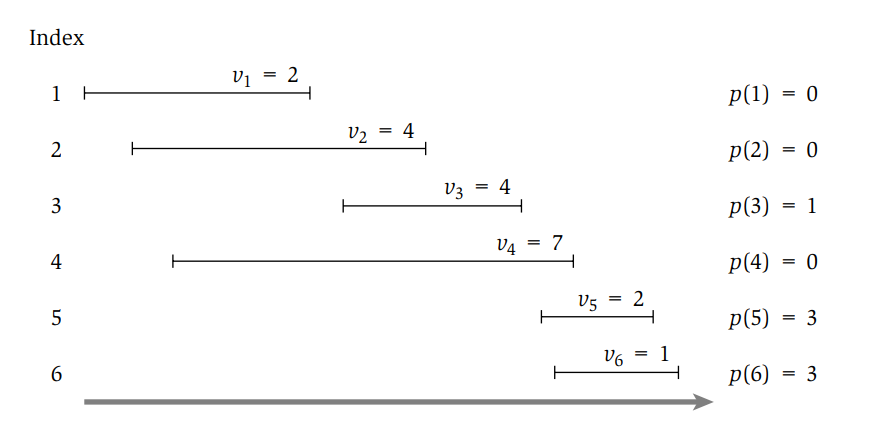
\includegraphics[width=12cm, keepaspectratio]{capitoli/imgs/weighted_problem.png}
    \caption{Istanza di un problema.}
\end{figure}

\section{Goal \normalfont{\emoji{soccer-ball}}}

L'obiettivo del nostro problema attuale è quello di trovare un sottoinsieme $S
    \subseteq \{1, \ldots, n\}$ di intervalli mutualmente compatibili che vanno a
massimizzare la somma dei pesi degli intervalli selezionati $\sum_{i \in S}
    v_i$.

\section{Funzionamento}

Come prima cosa definiamo il metodo per calcolare $OPT(j)$. Il problema è
una \textit{scelta binaria} che va a decidere se l'intervallo di indice $j$
verrà incluso nella soluzione oppure no basandosi sul valore ritornato dalla
seguente formula:

\begin{equation}
    \label{eqn:weight-opt}
    OPT(j) = max(v_j + OPT(p(j)), \ \ OPT(j-1))
\end{equation}
\ \\
Questo può essere anche visto come una disequazione:

\begin{equation}
    \label{eqn:weight-opt-dis}
    v_j + OPT(p(j)) \geq OPT(j-1)
\end{equation}
\ \\
che se vera, includerà $j$ nella soluzione ottimale.

\pagebreak

Scrivendo tutto sotto forma di algoritmo ricorsivo avremmo che:

\begin{lstlisting}[language=Javascript]
    function Compute-Opt(j){
        if (j == 0)
            return 0
        else
            return max(vj+Compute-Opt(p(j)), Compute-Opt(j − 1))
    }
\end{lstlisting}

Costruendo l'albero della ricorsione dell'algoritmo si nota che la complessità
temporale è esponenziale \emoji{astonished} !

\begin{figure}[H]
    \centering
    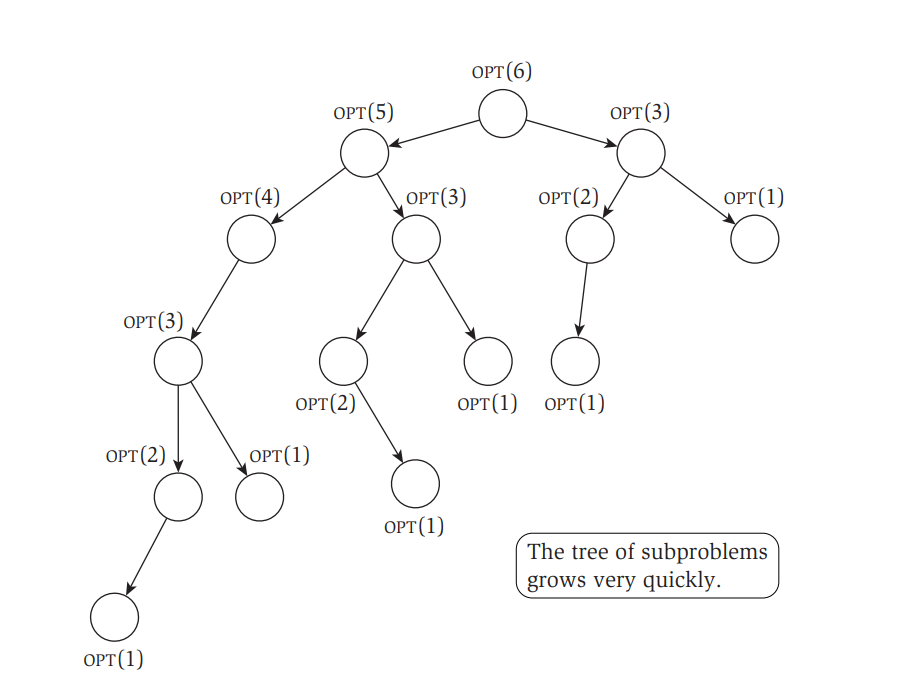
\includegraphics[width=12cm, keepaspectratio]{capitoli/imgs/opt_albero.png}
    \caption{Sviluppo dell'albero di ricorsione per la risoluzione di un problema.}
\end{figure}

\pagebreak

Una soluzione è quella di utilizzare la tecnica della \textbf{Memoization} che evita
di ricalcolare $OPT$ per gli indici già calcolati precedentemente, rendendo così
il costo temporale uguale ad $O(n)$ \emoji{man-in-motorized-wheelchair}.

\begin{lstlisting}[language=Javascript]
function M-Compute-Opt(j){
    if (j == 0)
        return 0
    else if (M[j] is not empty)
        return M[j]
    else
        let M[j] = max(vj+M-Compute-Opt(p(j)), M-Compute-Opt(j-1))
        return M[j]
}
\end{lstlisting}

Oltre al valore della soluzione ottimale probabilmente vorremmo sapere anche
quali sono gli intervalli che la compongono, e intuitivamente verrebbe da creare
un array aggiuntivo in cui verranno aggiunti gli indici degli intervalli
ottenuti con \verb|M-Compute-Opt|. Tuttavia questo aggiungerebbe una complessità
temporale di $O(n)$ peggiorando notevolmente le prestazioni. Un'alternativa è
quella di recuperare le soluzioni dai valori salvati nell'array \verb|M| dopo che la
soluzione ottimale è stata calcolata. Per farlo possiamo sfruttare la formula
vista in precedenza $v_j + OPT(p(j)) \geq OPT(j-1)$, che ci permette di
rintracciare gli intervalli della soluzione ottima.

\begin{lstlisting}[language=Javascript]
    function Find-Solution(j) {
        if (j == 0)
            Output nothing
        else if (vj + M[p(j)] >= M[j-1])
            Output j together with the result 
            of Find-Solution(p(j))
        else
            Output the result of Find-Solution(j-1)
    }
\end{lstlisting}
% \chapter{Least Squares Problem: Multi-way Choice \normalfont{\emoji{motorway}}}

Nel capitolo precedente l'algoritmo richiedeva una ricorsione basata su scelte
binarie, in questo capitolo invece introdurremo un algoritmo che richiede ad
ogni step un numero di scelte polinomiali (\textit{multi-way choice}). Vedremo
come la programmazione dinamica si presta molto bene a risolvere questi
problemi.

\section{Linear Least Square}

\subsection{Il Problema}

La formulazione del problema è la seguente:

\paragraph*{} dato un insieme $P$ composto di $n$ punti sul piano denotati con\\
$(x_1, y_1), (x_2, y_2), \ldots, (x_n, y_n)$; e supponiamo che $x_1 < x_2 <
    \ldots < x_n$ (sono strettamente crescenti). Data una linea $L$ definita
dall'equazione $y = ax + b$, definiamo l'\textit{errore} di $L$ in funzione
di $P$ come la somma delle distanze al quadrato della linea rispetto ai
punti in $P$. Formalmente:
\[
    Error(L, P) = \sum_{i=1}^{n} (y_i - ax_i - b)^2
\]

\begin{figure}[H]
    \centering
    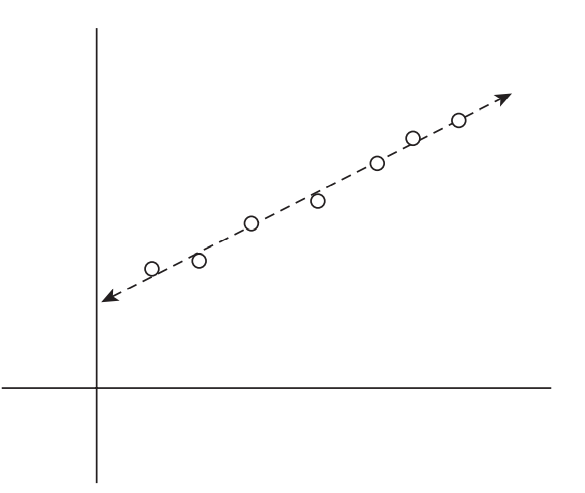
\includegraphics[width=6cm, keepaspectratio]{capitoli/imgs/linear_least.png}
    \caption{Esempio di una tipica istanza e soluzione del problema
        \textit{Linear Least}}
\end{figure}

\subsection{\goal}

È intuibile che il goal dell'algoritmo è quello di cercare la linea con errore
minimo, che può essere facilmente trovata utilizzando l'analisi matematica.
La linea di errore minimo è $y = ax + b$ dove:

\[
    a = \frac{n \sum_{i} x_i y_i - (\sum_{i} x_i) (\sum_{i} y_i)}{n \sum_{i} x_i^2 - (\sum_{i} x_i)^2} \ \ \  \ \ b = \frac{\sum_{i} y_i - a \sum_{i} x_i}{n}
\]

\section{Segmented Least Square}

Le formule appena citate sono utilizzabili solo se i punti di $P$ hanno un
andamento che è abbastanza lineare ma falliscono in altre circostanze.

\begin{figure}[H]
    \centering
    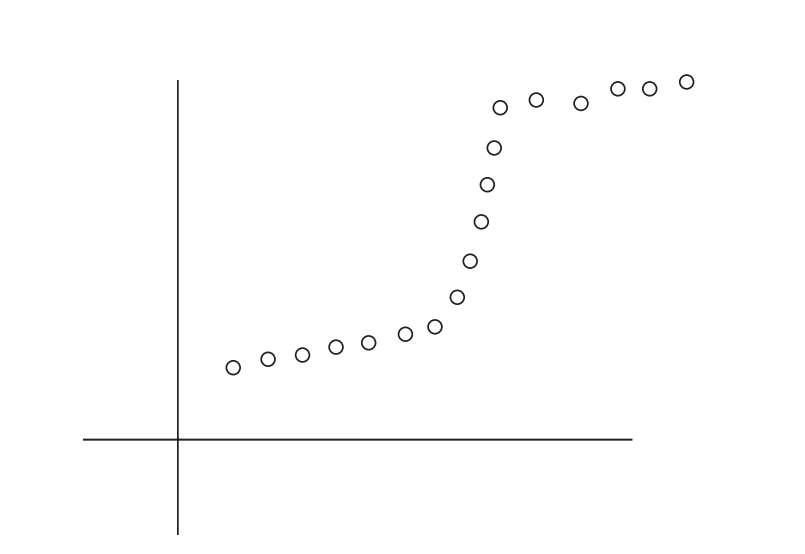
\includegraphics[width=8cm, keepaspectratio]{capitoli/imgs/segmente_linear_least.png}
    \caption{Esempio di funzione non risolvibile con Linear Least Square}
\end{figure}

Come è evidente (\textit{lapalissiano \normalfont{\emoji{gem}}}) dalla figura
non è possibile trovare una linea che approssimi in maniera soddisfacente i
punti, dunque per risolvere il problema possiamo pensare di rilassare la
condizione che sia solo una la linea. Questo però implica dover riformulare il
goal che altrimenti risulterebbe banale (si fanno $n$ linee che passano per ogni
punto).

\subsection{Costi}

La parte che computa gli errori ha costo in tempo $O(n^3)$ (si può portare a
$O(n^2)$).
La parte che trova il valore ottimo ha costo $O(n^2)$.\\

In spazio l'algoritmo ha costo $O(n^2)$ ma può essere ridotto a $O(n)$

\subsection{\goal}

Formalmente, il problema è espresso come segue:

\paragraph*{} come prima abbiamo un set di punti $P = \{(x_1, y_1), (x_2, y_2),
    \ldots, (x_n, y_n)\}$ strettamente crescenti. Denoteremo l'insieme dei punti
$(x_i, y_i)$ con $p_i$. Vogliamo partizionare $P$ in un qualche numero di
segmenti, ogni numero di segmenti è un sottoinsieme di $P$ che rappresenta un
\textit{set} contiguo delle coordinate $x$ con la forma $\{p_i, p_{i+1}, \ldots,
    p_{j-1}, p_j\}$ per degli indici $i \leq j$. Dopodiché, per ogni segmento $S$
calcoliamo la linea che minimizza l'errore rispetto ai punti in $S$ secondo
quanto espresso dalle formule enunciate prima.\\

Definiamo infine una penalità per una data partizione come la somma dei seguenti
termini:

\begin{itemize}
    \item Numero di segmenti in cui viene partizionato $P$ moltiplicato per un
          valore $C > 0$ (più è grande e più penalizza tante partizioni)
    \item Per ogni segmento l'errore della linea ottima attraverso quel
          segmento.
\end{itemize}


Il goal del Segmented Least Square Problem è quindi quello di trovare la
partizione di \textbf{penalità minima}.

\subsection{Funzionamento}

Per come è fatta la programmazione dinamica noi vogliamo suddividere il problema
in sotto-problemi e per farlo partiamo dall'osservazione che l'ultimo punto
appartiene ad una partizione ottima che parte da un valore $p_i$ fino a $p_n$ e
che possiamo togliere questi punti dal totale per ottenete un sotto-problema più
piccolo. Supponiamo che la soluzione ottima sia denotata da \verb|OPT(j)|, per i
punti che vanno da $p_1$ a $p_j$, allora avremo che la soluzione ottima al
problema dato l'ultimo segmento che va da $p_i$ a $p_n$, sarà dalla seguente
formula:

\[
    OPT(n) = e_{i,n} + C + OPT(i - 1)
\]

Questa formula è data dalla soluzione ottima dell'ultima partizione ($e_{i,n} + C$)
a cui viene aggiunta la soluzione ottima di tutte le partizioni precedenti
($OPT(i -1)$). Per i sotto-problemi possiamo scrivere la soluzione al problema
in forma ricorsiva utilizzando la formula appena espressa che prenderà la forma:

\[
    OPT(j) = \min_{1 \leq i \leq j}(e_{i,j} + C + OPT(i - 1))
\]

Possiamo ora dare una versione di questo algoritmo in pseudocodice:

\begin{lstlisting}[language=Javascript]
    function Segmented-Least-Squares(n) {
        M[0 ... n]
        M[0] = 0

        // compute the errors
        for (j in 1 ... n) {
            for (i in 1 ... j) {
                compute eij for the segment pi, ..., pj
            }
        }

        // find optimal value
        for (j in 1 ... n) {
            M[j] = min_i(eij + C + M[i - 1]) // OPT(J)
        }

        return M[n]
    }
\end{lstlisting}

Dopo aver trovato la soluzione ottima, possiamo sfruttare la memoization per
ricavarci i segmenti in tempi brevi.

\begin{lstlisting}[language=Javascript]
    function Find-Segments(j) {
        if (j == 0) print('')

        else {
            Find an i that minimizes ei,j + C + M[i − 1]
            Output the segment {pi,..., pj} and the result of Find-Segments(i − 1)
        }
    }
\end{lstlisting}

L'algoritmo ha costo $O(n^3)$ in tempo e $O(n^2)$ in spazio.
Questo tempo può essere ridotto applicando la memoization alle formule per il calcolo
dell'errore viste in precedenza portandolo a $O(n^2)$ per il tempo e $O(n)$ per lo spazio.
% \chapter{Subset Sum \& Knapsack Problem \normalfont{\emoji{money-bag}}}

\section{Il Problema}

Il problema delle Subset Sum è formalmente definito come segue:\\

\- abbiamo $n$ oggetti $\{1, \ldots, n\}$, a ognuno viene assegnato un
peso non negativo $w_i$ (per $i = 1, \ldots, n$) e ci viene dato anche un
limite $W$. L'obbiettivo è quello di selezionare un sottoinsieme $S$ degli
oggetti tale che $\sum_{i \in S}w_i \leq W$ e che questa sommatoria abbia valore
più grande possibile.\\

Questo problema è un caso specifico di un problema più generale conosciuto come
il Knapsack Problem, l'unica differenza sta nel valore da massimizzare che per il
Knapsack è un valore $v_i$ e non più il peso.

Si potrebbe pensare di risolvere questi problemi con un algoritmo greedy ma
purtroppo non ne esiste uno in grado di trovare efficientemente la soluzione ottima.
Potremmo pensare di ordinare gli oggetti in base al peso in ordine crescente o
decrescente e prenderli, tuttavia questo approccio fallisce per determinati casi
(come per l'insieme $\{W/2+1, W/2, W/2\}$ ordinato in senso decrescente) e l'unica
opzione sarà quella di provare con la programmazione dinamica \emoji{person-in-manual-wheelchair}.
\newpage

\section{\goal}

Possiamo riassumere il goal di questi problemi come segue:\\

\- Abbiamo $n$ oggetti $\{1, \ldots, n\}$, a ognuno viene assegnato un
peso non negativo $w_i$ (per $i = 1, \ldots, n$) e ci viene dato anche un
limite $W$. L'obbiettivo è quello di selezionare un sottoinsieme $S$ degli oggetti
tale che $\sum_{i \in S}w_i \leq W$ e che questa sommatoria abbia valore più
grande possibile.

\section{Costi}

\begin{center}
    \begin{tabular}{|c|c|}
        \centering
        \textbf{Funzione}    & \textbf{Costo (tempo)} \\
        \verb|Subset-Sum|    & $O(nW)$                \\
        \verb|Find-Solution| & $O(n)$                 \\
    \end{tabular}
\end{center}

\section{Funzionamento}

Come per tutti gli algoritmi dinamici dobbiamo cercare dei sotto-problemi e
possiamo utilizzare la stessa intuizione avuto per il problema dello scheduling
(scelta binaria). Facendo tutti i calcoli di dovere otteniamo la seguente
ricorsione:

\begin{center}
    se $w < w_i$ allora $OPT(i, w) = OPT(i-1,w)$ altrimenti\\
    $OPT(i, w) = max(OPT(i-1, w), w_i + OPT(i-1, w-w_i))$
\end{center}

Nella prima parte analizziamo il caso in cui l'elemento che vogliamo aggiungere va
a superare il peso massimo residuo $w$, dunque viene scartato. Nella seconda parte
andiamo ad analizzare se l'aggiunta o meno del nuovo oggetto va a migliorare
la soluzione di $OPT$ che è definita come:\\

\[
    OPT(i, w) = \max_{S} \sum_{j \in S} w_j
\]
\newpage

Possiamo formalizzare il tutto con il seguente pseudo-codice:

\begin{lstlisting}[language=JavaScript]
    function Subset-Sum(n, W) {
        let M[0 . . . n,0... W]

        //initialize the memoization vector
        for(w in 0 ... W) {
            M[0, W] = 0
        }

        //solve subproblems
        for(i in 1 ... n) {
            for(w in 0 ... W) {
                Use the recurrence to compute M[i, w]
            }
        }

        return M[n, W]
    }
\end{lstlisting}

La particolarità di questo algoritmo è che avremmo 2 insiemi di sotto-problemi
diversi che devono essere risolti per ottenere la soluzione ottima. Questo fatto
si riflette in come viene popolato l'array di memoization dei valori di $OPT$
che verranno salvati in un array bidimensionale.

\begin{figure}[H]
    \centering
    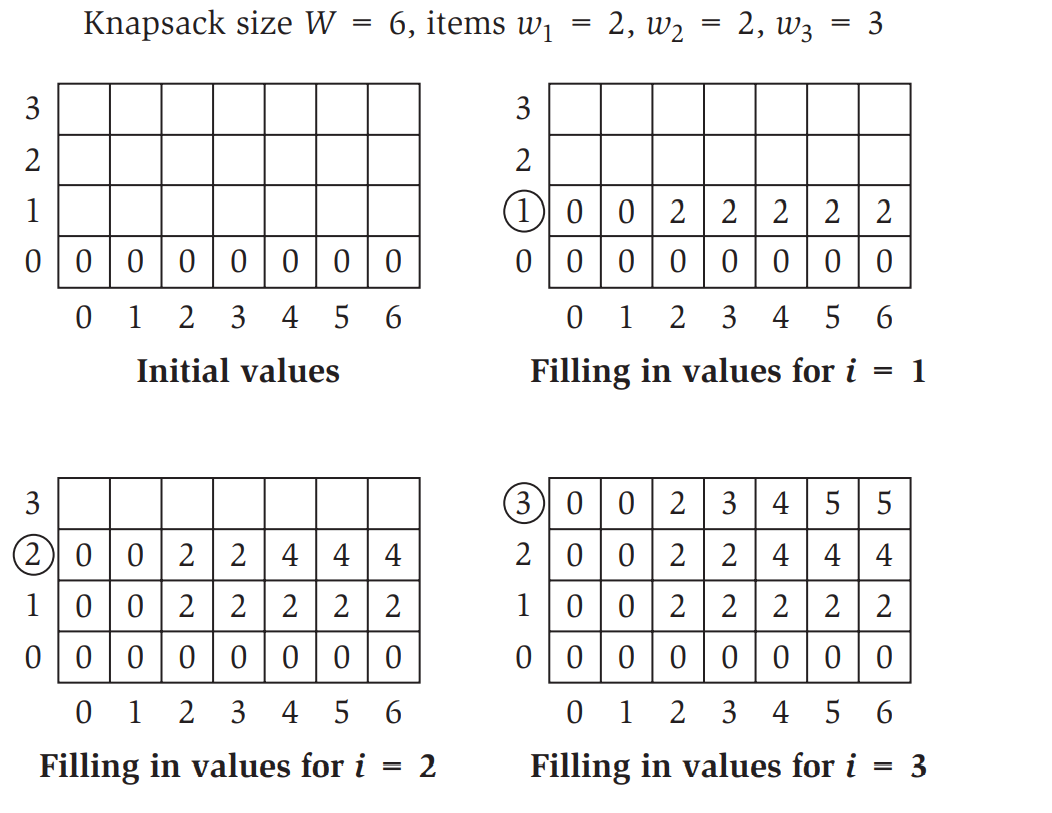
\includegraphics[width=10cm, keepaspectratio]{capitoli/imgs/knapsac_table.png}
    \caption{Esempio di come viene popolato l'array $M$ per il problema del Knapsack.}
\end{figure}

\textit{Il costo in tempo di questa implementazione è di $O(nW)$.}\\

A causa di questo costo, l'algoritmo fa parte della famiglia degli
algoritmi \textit{pseudo polinomiali}, ovvero algoritmi il cui costi dipende da
una variabile di input che se piccola, lo mantiene basso e se grande lo fa
esplodere.\\

\textit{Per recuperare gli oggetti dall'array di Memoization la complessità in tempo è di
    $O(n)$.}\\

Questa implementazione funziona anche per il problema più generale del Knapsack,
ci basterà solo cambiare la parte di ricorsione scrivendola come segue:

\begin{center}
    se $w < w_i$ allora $OPT(i, w) = OPT(i-1,w)$ altrimenti
    $OPT(i, w) = max(OPT(i-1, w), v_i + OPT(i-1, w-w_i))$
\end{center}

La complessità temporale è sempre $O(nW)$.
% \section{RNA Secondary Structure \normalfont{\emoji{dna}}}

La ricerca della struttura secondaria dell'RNA è un problema a 2 variabili
risolvibile tramite il paradigma della programmazione dinamica. Come sappiamo il
DNA è composto da due filamenti, mentre l'RNA è composto da un filamento
singolo. Questo comporta che spesso le basi di un singolo filamento di RNA si
accoppino tra di loro. L'insieme della basi può essere visto come l'alfabeto
$\{A, C, U, G\}$ e l'RNA è una sequenza di simboli presi da questo alfabeto. Il
processo di accoppiamento delle basi è dettato dalla regola di \textit{Watson-Crick} e
segue il seguente schema:

\[
    A - U \ \ \ \textrm{ e } \ \ \ C - G \ \ \ \textrm{ (l'ordine non conta)}
\]

\begin{figure}[H]
    \centering
    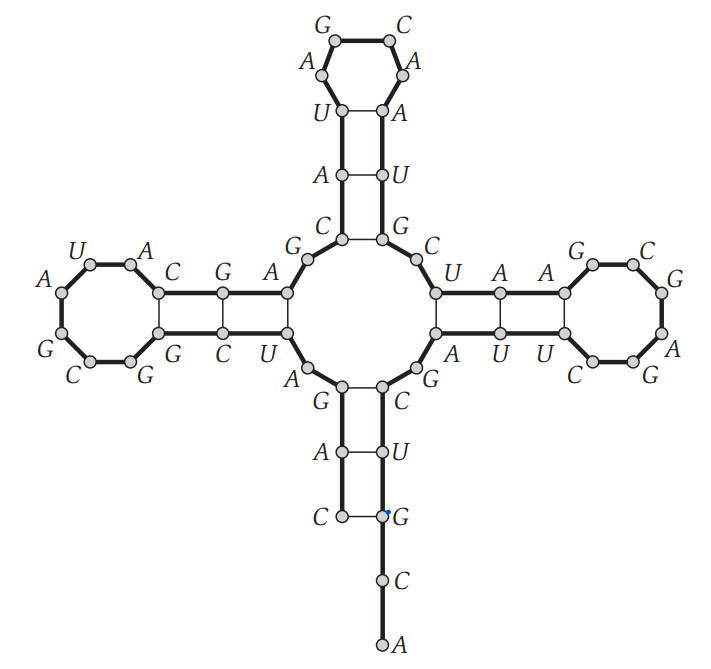
\includegraphics[width=8cm, keepaspectratio]{capitoli/dynamic_programming/imgs/rna_esempio1.png}
    \caption{Esempio di una struttura secondari di RNA} %%TODO: ricontrollare !!
\end{figure}

\subsection{Il Problema}

In questo problema si vuole trovare la struttura secondaria dell'RNA che abbia
energia libera maggiore (il maggior numero di coppie di basi possibili). Per
farlo dobbiamo tenere in considerazione alcune condizioni che devono essere
soddisfatte per permettere di approssimare al meglio il modello biologico
dell'RNA.\\

Formalmente la struttura secondaria di $B$ è un insieme di coppie $S =
    \{(i,j)\}$ dove $i,j \in \{1,2,\ldots,n\}$, che soddisfa le seguenti
condizioni:

\begin{enumerate}
    \item \textbf{No Sharp Turns}: la fine di ogni coppia è separata da almeno 4
          basi, quindi se $(i,j) \in S$ allora $i < j - 4$
    \item Gli elementi di una qualsiasi coppia $S$ consistono di $\{A, U\}$ o
          $\{C, G\}$ (in qualsiasi ordine).
    \item $S$ è un \textit{matching}: nessuna base compare in più di una coppia.
    \item \textbf{Non Crossing Condition}: se $(i, j)$ e $(k,l)$ sono due coppie
          in $S$ allora \textbf{non} può avvenire che $i < k < j < l$.
\end{enumerate}

\begin{figure}[H]
    \centering
    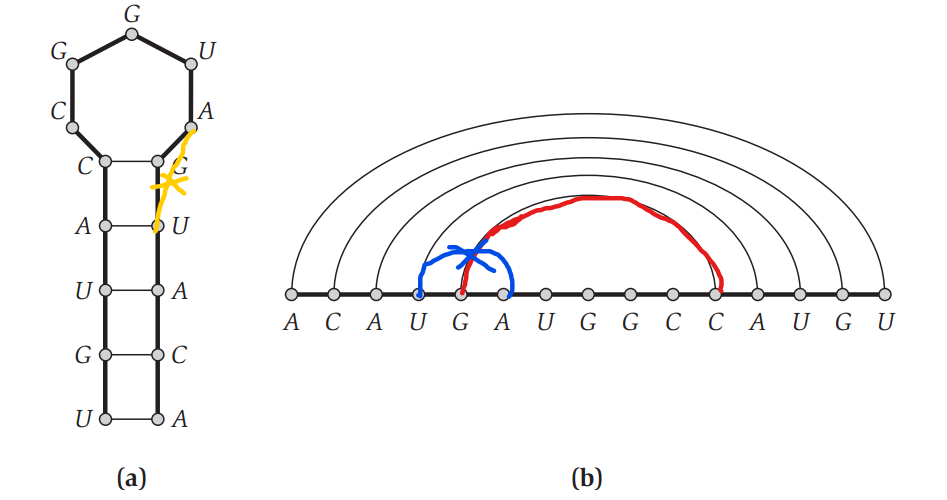
\includegraphics[width=10cm, keepaspectratio]{capitoli/dynamic_programming/imgs/rna_esempio2.png}
    \caption{La figura \textit{(a)} rappresenta un esempio di \textit{Sharp
            Turn}, mentre la figura \textit{(b)} mostra una
        \textit{Crossing Condition} dove il filo blu non dovrebbe esistere.}
\end{figure}

\subsection{\goal}

Il goal di questo problema è di massimizzare la quantità di coppie che si possono
formare all'interno della struttura secondaria di una data sequenza di RNA.

\subsection{Costi}

L'algoritmo complessivo ha costo $O(n^3)$.

\subsection{Funzionamento}

\paragraph{First Attempt.}
Come primo tentativo potremmo basarci sul seguente sotto-problema: affermiamo che
$OPT(j)$ è il massimo numero di coppie di basi sulla struttura secondaria $b_1
    b_2 \ldots b_j$, per la Non Sharp Turn Condition sappiamo che $OPT(j) = 0$ per
$j \leq 5$ e sappiamo anche che $OPT(n)$ è la soluzione che vogliamo trovare. Il
problema ora sta nell'esprimere $OPT(j)$ ricorsivamente. Possiamo parzialmente
farlo sfruttando le seguenti scelte:

\begin{itemize}
    \item $j$ non appartiene ad una coppia
    \item $j$ si accoppia con $t$ per qualche $t \leq
              j - 4$
\end{itemize}

Per il primo caso basta cercare la soluzione per $OPT(j - 1)$, nel secondo caso
invece se teniamo conto della Non Crossing Condition, possiamo isolare due nuovi
sotto-problemi: uno sulle basi $b_1 b_2 \ldots b_{t-1}$ e l'altro sulle basi
$b_{t+1} \ldots b_{j-1}$. Il primo si risolve con $OPT(t-1)$ ma il secondo, dato
che non inizia con indice $1$, non è nella lista dei nostri sotto-problemi. A
causa di ciò risulta necessario aggiungere una variabile.

\begin{figure}[H]
    \centering
    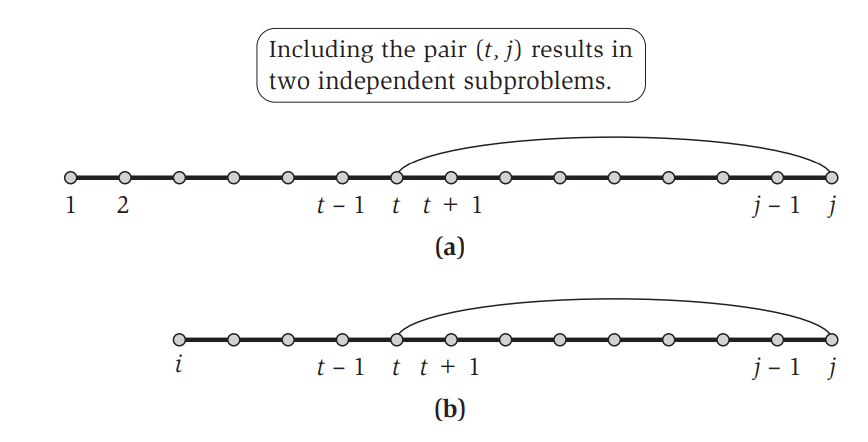
\includegraphics[width=10cm, keepaspectratio]{capitoli/dynamic_programming/imgs/rna_funzionamento.png}
    \caption{Esempio di
        utilizzo di una sola variabile \textit{(a)} o con due \textit{(b)}.}
\end{figure}

\paragraph{Dynamic Programming over Intervals}
Basandoci sui ragionamenti precedenti, possiamo scrivere una ricorsione di
successo: sia $OPT(i,j)$ il numero massimo di coppie di basi nella struttura
secondaria $b_i b_{i+1} \ldots b_j$, grazie alla non sharp turn Condition
possiamo inizializzare gli elementi con $i \geq j -4$ a $0$. Ora avremmo sempre
le stesse condizioni elencate sopra:

\begin{itemize}
    \item $j$ non appartiene ad una coppia
    \item $j$ si accoppia con $t$ per qualche $t \leq j - 4$
\end{itemize}

Nel primo caso avremmo che $OPT(i,j) = OPT(i, j-1)$, nel secondo caso possiamo
ricorrere su due sotto-problemi $OPT(i, t-1)$ e $OPT(t+1, j-1)$ affinché venga
rispettata la non crossing condition. Possiamo esprimere formalmente la
ricorsione come segue:

\begin{center}
    \[
        OPT(i, j) = \max(OPT(i, j-1), \max_t(1+OPT(i, t-1)+OPT(t+1, j-1))),
    \]
    dove il massimo è calcolato su $t$ tale che $b_t$ e $b_j$ siano una coppia di
    basi consentita
\end{center}

\begin{figure}[H]
    \centering
    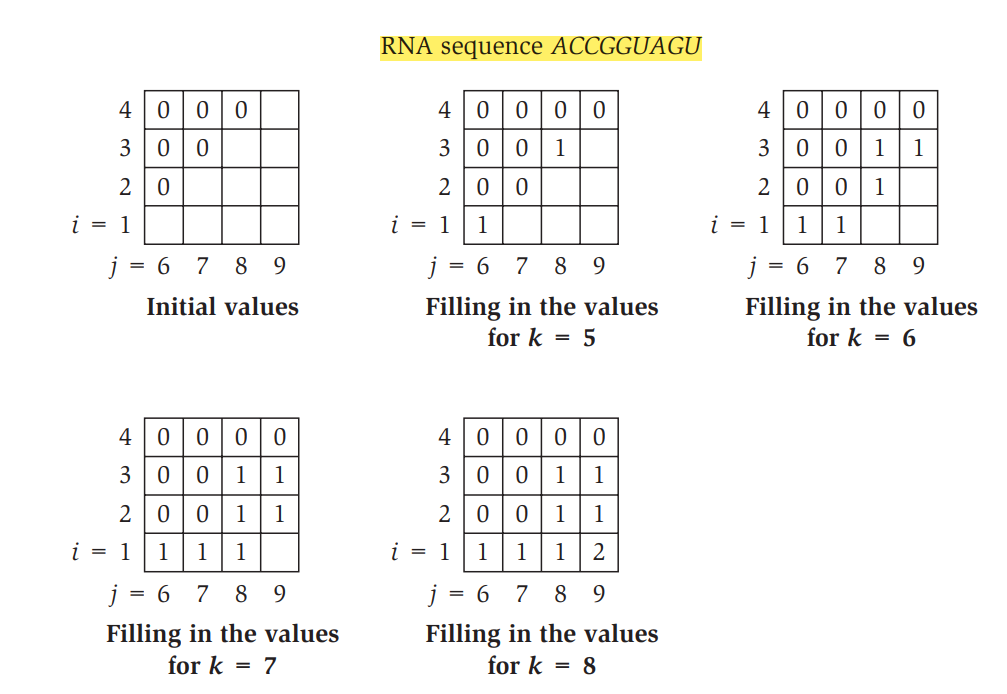
\includegraphics[width=\textwidth, keepaspectratio]{capitoli/dynamic_programming/imgs/rna_calcolo.png}
    \caption{Iterazioni dell'algoritmo su un campione del problema in questione $ACCGGUAGU$}
\end{figure}
\newpage

Possiamo infine formalizzare il tutto con il seguente pseudo-codice:

\begin{lstlisting}[language=JavaScript]
 Initialize OPT(i, j) = 0 whenever i ≥ j - 4

 for (k in 5 ... n - 1) {
     for (i in 1 ... n - k) {
         j = i + k
         Compute OPT(i, j) using the previous recurrence
     }
 }

 return OPT(1, n)
\end{lstlisting}

Ci sono $O(n^2)$ sotto-problemi da risolvere e ognuno richiede tempo $O(n)$,
quindi il running time complessivo è di $O(n^3)$.

% \section{Sequence Alignment}

Il problema del Sequence Alignment consiste nel riuscire a comparare delle
stringhe, come per esempio quando si effettua un typo in un motore di ricerca e
quello ci fornisce l'alternativa corretta. Una prima idea potrebbe essere quella
di \textbf{allineare} le due parole lettera per lettera, riempendo gli eventuali
spazi bianchi, e vedendo di quanto le due differiscono. Tuttavia ci sono varie
possibilità con cui due parole di lunghezza diversa possono essere confrontate,
quindi è necessario fornire una definizione di \textbf{similarità}.

\subsection{Il Problema}

Come prima definizione di similarità possiamo dire che minore sarà il numero di
caratteri che non corrispondono, maggiore sarà la similarità tra le parole.
Questa problematica è anche un tema centrale della biologia molecolare, e
proprio grazie ad un biologo abbiamo una definizione rigorosa e soddisfacente di
similarità. Prima di dare una definizione similarità dovremo però darne una di
\textbf{allineamento}: Supponiamo di avere due stringhe $X$ e $Y$, che consistono rispettivamente
della sequenza di simboli $x_1 x_2 \ldots x_m$ e $y_1 y_2 \ldots y_n$, e
consideriamo gli insiemi $\{1,2,\ldots ,m\}$ e $\{1,2,\ldots ,n\}$ che
rappresentano le varie posizioni nelle stringhe $X$ e $Y$, ora si considera un
\textbf{Matching} di queste due parole (un matching è stato definito nella parte
precedente e si tratta di un insieme di coppie ordinate con la proprietà che
ogni oggetto si trova al più in una sola coppia).  Diciamo ora che un matching
$M$ di questi due insiemi è un allineamento se gli elementi di varie coppie non
si incrociano: se $(i,j),(i^{\prime},j^{\prime}) \in M$  e $i < i^{\prime}$,
allora $j < j^{\prime}$.\\

Ora la nostra definizione di similarità si baserà sul trovare il miglior
allineamento, seguendo i seguenti criteri:

\begin{itemize}
    \item C'è un parametro $\delta>0$ che
          definisce la \textbf{gap penalty}, ovvero ogni volta che un simbolo di una parola
          non corrisponde ad un simbolo dell'altra.
    \item Per ogni coppia di lettere $p,q$ del
          nostro alfabeto, se c'è un accoppiamento errato si paga il corrispondente
          \textbf{mismatch cost} $a_(p,q)$.
    \item Il costo di $M$ è la somma del suo gap e mismatch
          cost, e l'obiettivo sarà quello di minimizzarlo.
\end{itemize}

\subsection{Creazione dell'algoritmo}

Ora affronteremo il problema di calcolarci questo costo minimo, e l'allineamento
ottimale che lo fornisce date le coppie $X$ e $Y$. Come al solito proveremo con
un approccio di programmazione dinamica, e per realizzare l'algoritmo
individuiamo come per altri algoritmi già visti una scelta binaria. Dato
l'allineamento ottimale $M$ allora:

\begin{itemize}
    \item $(m,n) \in M$ (quindi gli ultimi due
          simboli delle 2 stringhe sono in un matching)
    \item $(m,n) \notin M$ (gli ultimi
          simboli delle due stringhe non sono in un matching)
\end{itemize}

Tuttavia questa semplice distinzione non è sufficiente, quindi supponiamo di
aggiungere anche il seguente fatto elementare:\\

\- Sia $M$ un qualsiasi allineamento di $X$ e $Y$. se $(m,n) \notin M$, allora o
l' $m-esima$ posizione di $X$ o l' $n-esima$ posizione di $Y$ non è in un
matching di $M$.\\

Dire questo equivale a riscrivere le due condizioni sopra come tre, dunque in un
allineamento ottimo $M$ almeno una deve essere vera:

\begin{itemize}
    \item $(m,n) \in M$
    \item l'$m-esima$ posizione di $X$ non è nel matching
    \item l' $n-esima$ posizione di $Y$ non è nel matching
\end{itemize}

Ora definiamo la funzione di costo minimo $OPT(i,j)$ come costo dell'alignmet
tra $x_1 x_2 \ldots x_i$ e $y_1 y_2 \ldots y_j$. In base alle condizioni
espresse in precedenza la funzione $OPT(m,n)$ assumerà il costo relativo più
$OPT(m-1,n-1)$, in particolare (i tre casi citati sopra):

\begin{itemize}
    \item condizione 1, si
          paga un matching cost per le lettere $m,n$
    \item condizione 2 e 3, si paga un gap
          cost $\delta$ per $m$(condizione 2) o $n$(condizione 3)
\end{itemize}

Utilizzando dunque gli stessi argomenti per per i sotto problemi per
l'allineamento di costo minimo tra $X$ e $Y$ otteniamo la definizione generale
di $OPT(i,j)$:\\

L'allineamento di costo minimo soddisfa la seguente ricorsione per $i \geq 1$
e $j \geq 1$:
\[
    OPT(i,j) = min[a_{(x_i y_j)} + OPT(i-1, j-1),
            \delta + OPT(i-1, j), \delta + OPT(i, j-1)]
\]

Dunque così abbiamo ottenuto la nostra funzione di ricorsione e possiamo
procedere alla scrittura dello pseudo codice.

\begin{lstlisting}[language=JavaScript]
    function alignment(X,Y) { var A = Matrix(m, n)

        Initialize A[i, 0]= iδ for each i 
        Initialize A[0, j]= jδ for each j

        for (j in 1...n) { 
            for (i in 1...m) { 
                Use the recurrence (6.16) to compute A[i, j] 
            }
        }

        return A[m, n]
    }
\end{lstlisting}

Il running time è di $O(mn)$

\subsection{Sequence Alignment in Spazio Lineare}

Come abbiamo appena visto l'algoritmo ha sia costo spaziale che temporale uguale
a $O(mn)$ e se come input consideriamo le parole della lingua inglese non
risulta essere un grande problema, ma se consideriamo genomi con 10 miliardi di
caratteri potrebbe risultare difficile poter lavorare con array di 10 GB \emoji{astonished}.
Questo problema può essere risolto utilizzando un approccio \textit{divide et impera}
che va a rendere lineare il costo dello spazio ( $O(n + m)$ ).

\subsubsection{Funzionamento}

Come prima cosa definiamo un algoritmo Space Efficient Alignment che ci permette
di trovare la soluzione ottima utilizzando il minor spazio possibile. Per farlo
notiamo che la funzione $OPT$ dipende solamente da una colonna precedente di
quella che si sta analizzando, dunque basterà caricarsi in memoria una matrice
$mx2$ riducendo così il costo spaziale ad $m$. Tuttavia utilizzando questo
metodo non e possibile ricurvare l'alignment effettivo perché non ci bastano le
informazioni.\\

Lo pseudo-codice dell'algoritmo appena definito è il seguente:

\begin{lstlisting}[language=JavaScript]
    function Space-Efficient-Alignment(X,Y) {
        var B = Matrix(m, 2)

        // (just as in column 0 of A)
        Initialize B[i, 0]= iδ for each i 

        for (j in 1...n) {
            B[0, 1]= jδ (since this corresponds to entry A[0, j])

            for (i in 1...m) {
                B[i, 1]= min[
                    αxiyj + B[i − 1, 0],
                    δ + B[i − 1, 1], 
                    δ + B[i, 0]
                ]
            }

            Move column 1 of B to column 0 to make room 
            for next iteration:
            Update B[i, 0] = B[i, 1] for each i
        }
    }
\end{lstlisting}

Possiamo quindi utilizzare un approccio \textit{divide et impera} che incorpora 2
tecniche diverse di programmazione dinamica per sfruttare questo approccio
appena definito e riuscire a trovare anche l'alignment in spazio lineare.
Definiamo quindi due funzioni:

\begin{itemize}
    \item $f(i, j)$ : è la funzione definita per l'algoritmo di Sequence
          Alignment di base (analoga a $OPT(i,j)$ )
    \item $g(i, j)$ : è l'analogo al contrario di $f$ ed è definito dalla
          seguente funzione ricorsiva: per $i < m$ e $j < n$ : $g(i,j) =
              min[a_{x+1y+1} + g(i+1, j+1), \delta + g(i, j+1), \delta + g(i+1, j)]$
\end{itemize}

Possiamo notare che la ricorsione $f$ procede a ritroso partendo dal fondo
mentre la ricorsione $g$ procede in avanti partendo dall'inizio. Possiamo
sfruttare questo fatto per provare ad utilizzare lo Space Efficiente Sequence
Alignment Algorithm combinato ad un approccio \textit{divide et impera} e un array di
supporto $P$ per riuscire a calcolare il Sequence Alignment in spazio lineare,
aumentando solo di una costatane la complessità temporale.\\

Possiamo riassumere il tutto con il seguente pseudo-codice:

\begin{lstlisting}[language=JavaScript]
    function Divide-and-Conquer-Alignment(X,Y) {
        var m = length(X)
        var n = length(Y)

        if (m <= 2 or n <= 2) {
            Compute optimal alignment using Alignment(X,Y)
        }

        Space-Efficient-Alignment(X, Y[1 : n/2])
        Backward-Space-Efficient-Alignment(X, Y[n/2 + 1 : n])

        Let q be the index minimizing f(q, n/2) + g(q, n/2)
        Add (q, n/2) to global list P

        Divide-and-Conquer-Alignment(X[1 : q],Y[1 : n/2])
        Divide-and-Conquer-Alignment(X[q + 1 : n],Y[n/2 + 1:n])

        return P
    }
\end{lstlisting}

\begin{figure}[H]
    \centering
    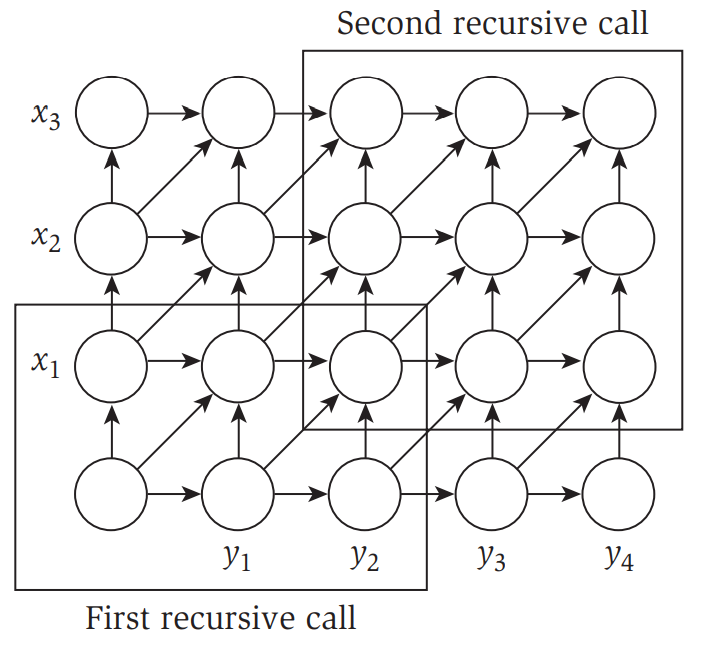
\includegraphics[width=8cm, keepaspectratio]{capitoli/dynamic_programming/imgs/seq_align_recurrence.png}
    \caption{La figura mostra il funzionamento dell'algoritmo appena descritto.}
\end{figure}

\documentclass[a4paper,12 pt]{report}
\usepackage[T1]{fontenc}
\usepackage[utf8]{inputenc}
% \usepackage{amsmath}
\usepackage{lmodern}
\usepackage{listings}
\usepackage{graphicx}
\usepackage{float}
\usepackage{subcaption}
\usepackage{hyperref}
\usepackage{wrapfig}
\usepackage{fancyhdr}
% \usepackage{tcolorbox}

% forza le footnote a stare il più in basso possibile
\usepackage[bottom]{footmisc}
\usepackage{enumitem}

%% STILE LISTINGS

\usepackage{xcolor}

\definecolor{codegreen}{rgb}{0,0.6,0}
\definecolor{codegray}{rgb}{0.5,0.5,0.5}
\definecolor{codepurple}{rgb}{0.58,0,0.82}
\definecolor{backcolour}{rgb}{0.95,0.95,0.92}

\lstdefinestyle{mystyle}{
    backgroundcolor=\color{backcolour},   
    commentstyle=\color{codegreen},
    keywordstyle=\color{magenta},
    numberstyle=\tiny\color{codegray},
    stringstyle=\color{codepurple},
    basicstyle=\ttfamily\footnotesize,
    breakatwhitespace=false,         
    breaklines=true,                 
    captionpos=b,                    
    keepspaces=true,                 
    numbers=left,                    
    numbersep=5pt,                  
    showspaces=false,                
    showstringspaces=false,
    showtabs=false,                  
    tabsize=2
}

\lstset{style=mystyle}

%% SOLIDITY Settings

% Copyright 2017 Sergei Tikhomirov, MIT License
% https://github.com/s-tikhomirov/solidity-latex-highlighting/

%\usepackage{listings, xcolor}

\definecolor{verylightgray}{rgb}{.97,.97,.97}

\lstdefinelanguage{Solidity}{
	keywords=[1]{anonymous, assembly, assert, balance, break, call, callcode, case, catch, class, constant, continue, constructor, contract, debugger, default, delegatecall, delete, do, else, emit, event, experimental, export, external, false, finally, for, function, gas, if, implements, import, in, indexed, instanceof, interface, internal, is, length, library, log0, log1, log2, log3, log4, memory, modifier, new, payable, pragma, private, protected, public, pure, push, require, return, returns, revert, selfdestruct, send, solidity, storage, struct, suicide, super, switch, then, this, throw, transfer, true, try, typeof, using, value, view, while, with, addmod, ecrecover, keccak256, mulmod, ripemd160, sha256, sha3}, % generic keywords including crypto operations
	keywordstyle=[1]\color{blue}\bfseries,
	keywords=[2]{address, bool, byte, bytes, bytes1, bytes2, bytes3, bytes4, bytes5, bytes6, bytes7, bytes8, bytes9, bytes10, bytes11, bytes12, bytes13, bytes14, bytes15, bytes16, bytes17, bytes18, bytes19, bytes20, bytes21, bytes22, bytes23, bytes24, bytes25, bytes26, bytes27, bytes28, bytes29, bytes30, bytes31, bytes32, enum, int, int8, int16, int24, int32, int40, int48, int56, int64, int72, int80, int88, int96, int104, int112, int120, int128, int136, int144, int152, int160, int168, int176, int184, int192, int200, int208, int216, int224, int232, int240, int248, int256, mapping, string, uint, uint8, uint16, uint24, uint32, uint40, uint48, uint56, uint64, uint72, uint80, uint88, uint96, uint104, uint112, uint120, uint128, uint136, uint144, uint152, uint160, uint168, uint176, uint184, uint192, uint200, uint208, uint216, uint224, uint232, uint240, uint248, uint256, var, void, ether, finney, szabo, wei, days, hours, minutes, seconds, weeks, years},	% types; money and time units
	keywordstyle=[2]\color{teal}\bfseries,
	keywords=[3]{block, blockhash, coinbase, difficulty, gaslimit, number, timestamp, msg, data, gas, sender, sig, value, now, tx, gasprice, origin},	% environment variables
	keywordstyle=[3]\color{violet}\bfseries,
	identifierstyle=\color{black},
	sensitive=false,
	comment=[l]{//},
	morecomment=[s]{/*}{*/},
	commentstyle=\color{gray}\ttfamily,
	stringstyle=\color{red}\ttfamily,
	morestring=[b]',
	morestring=[b]"
}

\lstdefinelanguage{JavaScript}{
  keywords={typeof, new, true, false, catch, function, return, null, catch, switch, var, if, in, while, do, else, case, break},
  keywordstyle=\color{blue}\bfseries,
  ndkeywords={class, export, boolean, throw, implements, import, this},
  ndkeywordstyle=\color{darkgray}\bfseries,
  identifierstyle=\color{black},
  sensitive=false,
  comment=[l]{//},
  morecomment=[s]{/*}{*/},
  commentstyle=\color{purple}\ttfamily,
  stringstyle=\color{red}\ttfamily,
  morestring=[b]',
  morestring=[b]"
}
%\lstset{
%	language=Solidity,
%	backgroundcolor=\color{verylightgray},
%	extendedchars=true,
%	basicstyle=\footnotesize\ttfamily,
%	showstringspaces=false,
%	showspaces=false,
%	numbers=left,
%	numberstyle=\footnotesize,
%	numbersep=9pt,
%	tabsize=2,
%	breaklines=true,
%	showtabs=false,
%	captionpos=b
%}

%% -----

% box around text
\newenvironment{boxed}
    {\begin{center}
    \begin{tabular}{|p{\textwidth}|}
    \hline\\
    }
    { 
    \\\\\hline
    \end{tabular} 
    \end{center}
    }

% Resetta la numerazione dei chapter quando
% una nuova part viene creata
\makeatletter
\@addtoreset{chapter}{part}
\makeatother

% Rimuove l'indentazione quando si crea un nuovo paragrafo
\setlength{\parindent}{0pt}

% footer
\pagestyle{fancyplain}
% rimuove la riga nell'header
\fancyhf{} % sets both header and footer to nothing
\renewcommand{\headrulewidth}{0pt}
\fancyfoot[L]{\href{https://github.com/Typing-Monkeys/AppuntiUniversita}{Typing Monkeys}}
\fancyfoot[C]{\emoji{gorilla}}
\fancyfoot[R]{\thepage}

% configurazione emoji
\usepackage{fontspec}
\usepackage{emoji}
\setemojifont{NotoColorEmoji.ttf}[Path=/usr/share/fonts/truetype/noto/]


% Macro
\newcommand{\goal}{Goal \normalfont{\emoji{soccer-ball}}}


\begin{document}
\include{frontmatter/main.tex}

%% TODO: riorganizzare la struttura degli appunti
%%       alla fine dovremmo avere una roba del tipo
%%          - Programmazione Dinamica
%%            - Arg 1
%%            - Arg 2
%%              - subarg 1
%%              - subarg 2
%%          - Flow
%%            - Arg 1
%%              - sub arg 1
%%          - Graph
%%            - Arg 1
%%

\tableofcontents

\include{quote/main.tex}

% \include{capitoli/dynamic_programming/1-introduzione_all_programmazione_dinamica.tex}
% \include{capitoli/dynamic_programming/2-weighted_interval_scheduling.tex}
% \include{capitoli/dynamic_programming/3-least_squares_problem_multiway_choice.tex}
% \include{capitoli/dynamic_programming/4-subset_sum_e_knapsack_problem.tex}
% \include{capitoli/dynamic_programming/5-rna_secondary_structure.tex}
% \include{capitoli/dynamic_programming/6-sequence_alignment.tex}
\include{capitoli/dynamic_programming/main.tex}

\end{document}

\end{document}

%% TODO: riorganizzare la struttura degli appunti
%%       alla fine dovremmo avere una roba del tipo
%%          - Programmazione Dinamica
%%            - Arg 1
%%            - Arg 2
%%              - subarg 1
%%              - subarg 2
%%          - Flow
%%            - Arg 1
%%              - sub arg 1
%%          - Graph
%%            - Arg 1
%%

\tableofcontents

\documentclass[a4paper,12 pt]{report}
\usepackage[T1]{fontenc}
\usepackage[utf8]{inputenc}
% \usepackage{amsmath}
\usepackage{lmodern}
\usepackage{listings}
\usepackage{graphicx}
\usepackage{float}
\usepackage{subcaption}
\usepackage{hyperref}
\usepackage{wrapfig}
\usepackage{fancyhdr}
% \usepackage{tcolorbox}

% forza le footnote a stare il più in basso possibile
\usepackage[bottom]{footmisc}
\usepackage{enumitem}

%% STILE LISTINGS

\usepackage{xcolor}

\definecolor{codegreen}{rgb}{0,0.6,0}
\definecolor{codegray}{rgb}{0.5,0.5,0.5}
\definecolor{codepurple}{rgb}{0.58,0,0.82}
\definecolor{backcolour}{rgb}{0.95,0.95,0.92}

\lstdefinestyle{mystyle}{
    backgroundcolor=\color{backcolour},   
    commentstyle=\color{codegreen},
    keywordstyle=\color{magenta},
    numberstyle=\tiny\color{codegray},
    stringstyle=\color{codepurple},
    basicstyle=\ttfamily\footnotesize,
    breakatwhitespace=false,         
    breaklines=true,                 
    captionpos=b,                    
    keepspaces=true,                 
    numbers=left,                    
    numbersep=5pt,                  
    showspaces=false,                
    showstringspaces=false,
    showtabs=false,                  
    tabsize=2
}

\lstset{style=mystyle}

%% SOLIDITY Settings

% Copyright 2017 Sergei Tikhomirov, MIT License
% https://github.com/s-tikhomirov/solidity-latex-highlighting/

%\usepackage{listings, xcolor}

\definecolor{verylightgray}{rgb}{.97,.97,.97}

\lstdefinelanguage{Solidity}{
	keywords=[1]{anonymous, assembly, assert, balance, break, call, callcode, case, catch, class, constant, continue, constructor, contract, debugger, default, delegatecall, delete, do, else, emit, event, experimental, export, external, false, finally, for, function, gas, if, implements, import, in, indexed, instanceof, interface, internal, is, length, library, log0, log1, log2, log3, log4, memory, modifier, new, payable, pragma, private, protected, public, pure, push, require, return, returns, revert, selfdestruct, send, solidity, storage, struct, suicide, super, switch, then, this, throw, transfer, true, try, typeof, using, value, view, while, with, addmod, ecrecover, keccak256, mulmod, ripemd160, sha256, sha3}, % generic keywords including crypto operations
	keywordstyle=[1]\color{blue}\bfseries,
	keywords=[2]{address, bool, byte, bytes, bytes1, bytes2, bytes3, bytes4, bytes5, bytes6, bytes7, bytes8, bytes9, bytes10, bytes11, bytes12, bytes13, bytes14, bytes15, bytes16, bytes17, bytes18, bytes19, bytes20, bytes21, bytes22, bytes23, bytes24, bytes25, bytes26, bytes27, bytes28, bytes29, bytes30, bytes31, bytes32, enum, int, int8, int16, int24, int32, int40, int48, int56, int64, int72, int80, int88, int96, int104, int112, int120, int128, int136, int144, int152, int160, int168, int176, int184, int192, int200, int208, int216, int224, int232, int240, int248, int256, mapping, string, uint, uint8, uint16, uint24, uint32, uint40, uint48, uint56, uint64, uint72, uint80, uint88, uint96, uint104, uint112, uint120, uint128, uint136, uint144, uint152, uint160, uint168, uint176, uint184, uint192, uint200, uint208, uint216, uint224, uint232, uint240, uint248, uint256, var, void, ether, finney, szabo, wei, days, hours, minutes, seconds, weeks, years},	% types; money and time units
	keywordstyle=[2]\color{teal}\bfseries,
	keywords=[3]{block, blockhash, coinbase, difficulty, gaslimit, number, timestamp, msg, data, gas, sender, sig, value, now, tx, gasprice, origin},	% environment variables
	keywordstyle=[3]\color{violet}\bfseries,
	identifierstyle=\color{black},
	sensitive=false,
	comment=[l]{//},
	morecomment=[s]{/*}{*/},
	commentstyle=\color{gray}\ttfamily,
	stringstyle=\color{red}\ttfamily,
	morestring=[b]',
	morestring=[b]"
}

\lstdefinelanguage{JavaScript}{
  keywords={typeof, new, true, false, catch, function, return, null, catch, switch, var, if, in, while, do, else, case, break},
  keywordstyle=\color{blue}\bfseries,
  ndkeywords={class, export, boolean, throw, implements, import, this},
  ndkeywordstyle=\color{darkgray}\bfseries,
  identifierstyle=\color{black},
  sensitive=false,
  comment=[l]{//},
  morecomment=[s]{/*}{*/},
  commentstyle=\color{purple}\ttfamily,
  stringstyle=\color{red}\ttfamily,
  morestring=[b]',
  morestring=[b]"
}
%\lstset{
%	language=Solidity,
%	backgroundcolor=\color{verylightgray},
%	extendedchars=true,
%	basicstyle=\footnotesize\ttfamily,
%	showstringspaces=false,
%	showspaces=false,
%	numbers=left,
%	numberstyle=\footnotesize,
%	numbersep=9pt,
%	tabsize=2,
%	breaklines=true,
%	showtabs=false,
%	captionpos=b
%}

%% -----

% box around text
\newenvironment{boxed}
    {\begin{center}
    \begin{tabular}{|p{\textwidth}|}
    \hline\\
    }
    { 
    \\\\\hline
    \end{tabular} 
    \end{center}
    }

% Resetta la numerazione dei chapter quando
% una nuova part viene creata
\makeatletter
\@addtoreset{chapter}{part}
\makeatother

% Rimuove l'indentazione quando si crea un nuovo paragrafo
\setlength{\parindent}{0pt}

% footer
\pagestyle{fancyplain}
% rimuove la riga nell'header
\fancyhf{} % sets both header and footer to nothing
\renewcommand{\headrulewidth}{0pt}
\fancyfoot[L]{\href{https://github.com/Typing-Monkeys/AppuntiUniversita}{Typing Monkeys}}
\fancyfoot[C]{\emoji{gorilla}}
\fancyfoot[R]{\thepage}

% configurazione emoji
\usepackage{fontspec}
\usepackage{emoji}
\setemojifont{NotoColorEmoji.ttf}[Path=/usr/share/fonts/truetype/noto/]


% Macro
\newcommand{\goal}{Goal \normalfont{\emoji{soccer-ball}}}


\begin{document}
\documentclass[a4paper,12 pt]{report}
\usepackage[T1]{fontenc}
\usepackage[utf8]{inputenc}
% \usepackage{amsmath}
\usepackage{lmodern}
\usepackage{listings}
\usepackage{graphicx}
\usepackage{float}
\usepackage{subcaption}
\usepackage{hyperref}
\usepackage{wrapfig}
\usepackage{fancyhdr}
% \usepackage{tcolorbox}

% forza le footnote a stare il più in basso possibile
\usepackage[bottom]{footmisc}
\usepackage{enumitem}

%% STILE LISTINGS

\usepackage{xcolor}

\definecolor{codegreen}{rgb}{0,0.6,0}
\definecolor{codegray}{rgb}{0.5,0.5,0.5}
\definecolor{codepurple}{rgb}{0.58,0,0.82}
\definecolor{backcolour}{rgb}{0.95,0.95,0.92}

\lstdefinestyle{mystyle}{
    backgroundcolor=\color{backcolour},   
    commentstyle=\color{codegreen},
    keywordstyle=\color{magenta},
    numberstyle=\tiny\color{codegray},
    stringstyle=\color{codepurple},
    basicstyle=\ttfamily\footnotesize,
    breakatwhitespace=false,         
    breaklines=true,                 
    captionpos=b,                    
    keepspaces=true,                 
    numbers=left,                    
    numbersep=5pt,                  
    showspaces=false,                
    showstringspaces=false,
    showtabs=false,                  
    tabsize=2
}

\lstset{style=mystyle}

%% SOLIDITY Settings

% Copyright 2017 Sergei Tikhomirov, MIT License
% https://github.com/s-tikhomirov/solidity-latex-highlighting/

%\usepackage{listings, xcolor}

\definecolor{verylightgray}{rgb}{.97,.97,.97}

\lstdefinelanguage{Solidity}{
	keywords=[1]{anonymous, assembly, assert, balance, break, call, callcode, case, catch, class, constant, continue, constructor, contract, debugger, default, delegatecall, delete, do, else, emit, event, experimental, export, external, false, finally, for, function, gas, if, implements, import, in, indexed, instanceof, interface, internal, is, length, library, log0, log1, log2, log3, log4, memory, modifier, new, payable, pragma, private, protected, public, pure, push, require, return, returns, revert, selfdestruct, send, solidity, storage, struct, suicide, super, switch, then, this, throw, transfer, true, try, typeof, using, value, view, while, with, addmod, ecrecover, keccak256, mulmod, ripemd160, sha256, sha3}, % generic keywords including crypto operations
	keywordstyle=[1]\color{blue}\bfseries,
	keywords=[2]{address, bool, byte, bytes, bytes1, bytes2, bytes3, bytes4, bytes5, bytes6, bytes7, bytes8, bytes9, bytes10, bytes11, bytes12, bytes13, bytes14, bytes15, bytes16, bytes17, bytes18, bytes19, bytes20, bytes21, bytes22, bytes23, bytes24, bytes25, bytes26, bytes27, bytes28, bytes29, bytes30, bytes31, bytes32, enum, int, int8, int16, int24, int32, int40, int48, int56, int64, int72, int80, int88, int96, int104, int112, int120, int128, int136, int144, int152, int160, int168, int176, int184, int192, int200, int208, int216, int224, int232, int240, int248, int256, mapping, string, uint, uint8, uint16, uint24, uint32, uint40, uint48, uint56, uint64, uint72, uint80, uint88, uint96, uint104, uint112, uint120, uint128, uint136, uint144, uint152, uint160, uint168, uint176, uint184, uint192, uint200, uint208, uint216, uint224, uint232, uint240, uint248, uint256, var, void, ether, finney, szabo, wei, days, hours, minutes, seconds, weeks, years},	% types; money and time units
	keywordstyle=[2]\color{teal}\bfseries,
	keywords=[3]{block, blockhash, coinbase, difficulty, gaslimit, number, timestamp, msg, data, gas, sender, sig, value, now, tx, gasprice, origin},	% environment variables
	keywordstyle=[3]\color{violet}\bfseries,
	identifierstyle=\color{black},
	sensitive=false,
	comment=[l]{//},
	morecomment=[s]{/*}{*/},
	commentstyle=\color{gray}\ttfamily,
	stringstyle=\color{red}\ttfamily,
	morestring=[b]',
	morestring=[b]"
}

\lstdefinelanguage{JavaScript}{
  keywords={typeof, new, true, false, catch, function, return, null, catch, switch, var, if, in, while, do, else, case, break},
  keywordstyle=\color{blue}\bfseries,
  ndkeywords={class, export, boolean, throw, implements, import, this},
  ndkeywordstyle=\color{darkgray}\bfseries,
  identifierstyle=\color{black},
  sensitive=false,
  comment=[l]{//},
  morecomment=[s]{/*}{*/},
  commentstyle=\color{purple}\ttfamily,
  stringstyle=\color{red}\ttfamily,
  morestring=[b]',
  morestring=[b]"
}
%\lstset{
%	language=Solidity,
%	backgroundcolor=\color{verylightgray},
%	extendedchars=true,
%	basicstyle=\footnotesize\ttfamily,
%	showstringspaces=false,
%	showspaces=false,
%	numbers=left,
%	numberstyle=\footnotesize,
%	numbersep=9pt,
%	tabsize=2,
%	breaklines=true,
%	showtabs=false,
%	captionpos=b
%}

%% -----

% box around text
\newenvironment{boxed}
    {\begin{center}
    \begin{tabular}{|p{\textwidth}|}
    \hline\\
    }
    { 
    \\\\\hline
    \end{tabular} 
    \end{center}
    }

% Resetta la numerazione dei chapter quando
% una nuova part viene creata
\makeatletter
\@addtoreset{chapter}{part}
\makeatother

% Rimuove l'indentazione quando si crea un nuovo paragrafo
\setlength{\parindent}{0pt}

% footer
\pagestyle{fancyplain}
% rimuove la riga nell'header
\fancyhf{} % sets both header and footer to nothing
\renewcommand{\headrulewidth}{0pt}
\fancyfoot[L]{\href{https://github.com/Typing-Monkeys/AppuntiUniversita}{Typing Monkeys}}
\fancyfoot[C]{\emoji{gorilla}}
\fancyfoot[R]{\thepage}

% configurazione emoji
\usepackage{fontspec}
\usepackage{emoji}
\setemojifont{NotoColorEmoji.ttf}[Path=/usr/share/fonts/truetype/noto/]


% Macro
\newcommand{\goal}{Goal \normalfont{\emoji{soccer-ball}}}


\begin{document}
\include{frontmatter/main.tex}

%% TODO: riorganizzare la struttura degli appunti
%%       alla fine dovremmo avere una roba del tipo
%%          - Programmazione Dinamica
%%            - Arg 1
%%            - Arg 2
%%              - subarg 1
%%              - subarg 2
%%          - Flow
%%            - Arg 1
%%              - sub arg 1
%%          - Graph
%%            - Arg 1
%%

\tableofcontents

\include{quote/main.tex}

% \include{capitoli/dynamic_programming/1-introduzione_all_programmazione_dinamica.tex}
% \include{capitoli/dynamic_programming/2-weighted_interval_scheduling.tex}
% \include{capitoli/dynamic_programming/3-least_squares_problem_multiway_choice.tex}
% \include{capitoli/dynamic_programming/4-subset_sum_e_knapsack_problem.tex}
% \include{capitoli/dynamic_programming/5-rna_secondary_structure.tex}
% \include{capitoli/dynamic_programming/6-sequence_alignment.tex}
\include{capitoli/dynamic_programming/main.tex}

\end{document}

%% TODO: riorganizzare la struttura degli appunti
%%       alla fine dovremmo avere una roba del tipo
%%          - Programmazione Dinamica
%%            - Arg 1
%%            - Arg 2
%%              - subarg 1
%%              - subarg 2
%%          - Flow
%%            - Arg 1
%%              - sub arg 1
%%          - Graph
%%            - Arg 1
%%

\tableofcontents

\documentclass[a4paper,12 pt]{report}
\usepackage[T1]{fontenc}
\usepackage[utf8]{inputenc}
% \usepackage{amsmath}
\usepackage{lmodern}
\usepackage{listings}
\usepackage{graphicx}
\usepackage{float}
\usepackage{subcaption}
\usepackage{hyperref}
\usepackage{wrapfig}
\usepackage{fancyhdr}
% \usepackage{tcolorbox}

% forza le footnote a stare il più in basso possibile
\usepackage[bottom]{footmisc}
\usepackage{enumitem}

%% STILE LISTINGS

\usepackage{xcolor}

\definecolor{codegreen}{rgb}{0,0.6,0}
\definecolor{codegray}{rgb}{0.5,0.5,0.5}
\definecolor{codepurple}{rgb}{0.58,0,0.82}
\definecolor{backcolour}{rgb}{0.95,0.95,0.92}

\lstdefinestyle{mystyle}{
    backgroundcolor=\color{backcolour},   
    commentstyle=\color{codegreen},
    keywordstyle=\color{magenta},
    numberstyle=\tiny\color{codegray},
    stringstyle=\color{codepurple},
    basicstyle=\ttfamily\footnotesize,
    breakatwhitespace=false,         
    breaklines=true,                 
    captionpos=b,                    
    keepspaces=true,                 
    numbers=left,                    
    numbersep=5pt,                  
    showspaces=false,                
    showstringspaces=false,
    showtabs=false,                  
    tabsize=2
}

\lstset{style=mystyle}

%% SOLIDITY Settings

% Copyright 2017 Sergei Tikhomirov, MIT License
% https://github.com/s-tikhomirov/solidity-latex-highlighting/

%\usepackage{listings, xcolor}

\definecolor{verylightgray}{rgb}{.97,.97,.97}

\lstdefinelanguage{Solidity}{
	keywords=[1]{anonymous, assembly, assert, balance, break, call, callcode, case, catch, class, constant, continue, constructor, contract, debugger, default, delegatecall, delete, do, else, emit, event, experimental, export, external, false, finally, for, function, gas, if, implements, import, in, indexed, instanceof, interface, internal, is, length, library, log0, log1, log2, log3, log4, memory, modifier, new, payable, pragma, private, protected, public, pure, push, require, return, returns, revert, selfdestruct, send, solidity, storage, struct, suicide, super, switch, then, this, throw, transfer, true, try, typeof, using, value, view, while, with, addmod, ecrecover, keccak256, mulmod, ripemd160, sha256, sha3}, % generic keywords including crypto operations
	keywordstyle=[1]\color{blue}\bfseries,
	keywords=[2]{address, bool, byte, bytes, bytes1, bytes2, bytes3, bytes4, bytes5, bytes6, bytes7, bytes8, bytes9, bytes10, bytes11, bytes12, bytes13, bytes14, bytes15, bytes16, bytes17, bytes18, bytes19, bytes20, bytes21, bytes22, bytes23, bytes24, bytes25, bytes26, bytes27, bytes28, bytes29, bytes30, bytes31, bytes32, enum, int, int8, int16, int24, int32, int40, int48, int56, int64, int72, int80, int88, int96, int104, int112, int120, int128, int136, int144, int152, int160, int168, int176, int184, int192, int200, int208, int216, int224, int232, int240, int248, int256, mapping, string, uint, uint8, uint16, uint24, uint32, uint40, uint48, uint56, uint64, uint72, uint80, uint88, uint96, uint104, uint112, uint120, uint128, uint136, uint144, uint152, uint160, uint168, uint176, uint184, uint192, uint200, uint208, uint216, uint224, uint232, uint240, uint248, uint256, var, void, ether, finney, szabo, wei, days, hours, minutes, seconds, weeks, years},	% types; money and time units
	keywordstyle=[2]\color{teal}\bfseries,
	keywords=[3]{block, blockhash, coinbase, difficulty, gaslimit, number, timestamp, msg, data, gas, sender, sig, value, now, tx, gasprice, origin},	% environment variables
	keywordstyle=[3]\color{violet}\bfseries,
	identifierstyle=\color{black},
	sensitive=false,
	comment=[l]{//},
	morecomment=[s]{/*}{*/},
	commentstyle=\color{gray}\ttfamily,
	stringstyle=\color{red}\ttfamily,
	morestring=[b]',
	morestring=[b]"
}

\lstdefinelanguage{JavaScript}{
  keywords={typeof, new, true, false, catch, function, return, null, catch, switch, var, if, in, while, do, else, case, break},
  keywordstyle=\color{blue}\bfseries,
  ndkeywords={class, export, boolean, throw, implements, import, this},
  ndkeywordstyle=\color{darkgray}\bfseries,
  identifierstyle=\color{black},
  sensitive=false,
  comment=[l]{//},
  morecomment=[s]{/*}{*/},
  commentstyle=\color{purple}\ttfamily,
  stringstyle=\color{red}\ttfamily,
  morestring=[b]',
  morestring=[b]"
}
%\lstset{
%	language=Solidity,
%	backgroundcolor=\color{verylightgray},
%	extendedchars=true,
%	basicstyle=\footnotesize\ttfamily,
%	showstringspaces=false,
%	showspaces=false,
%	numbers=left,
%	numberstyle=\footnotesize,
%	numbersep=9pt,
%	tabsize=2,
%	breaklines=true,
%	showtabs=false,
%	captionpos=b
%}

%% -----

% box around text
\newenvironment{boxed}
    {\begin{center}
    \begin{tabular}{|p{\textwidth}|}
    \hline\\
    }
    { 
    \\\\\hline
    \end{tabular} 
    \end{center}
    }

% Resetta la numerazione dei chapter quando
% una nuova part viene creata
\makeatletter
\@addtoreset{chapter}{part}
\makeatother

% Rimuove l'indentazione quando si crea un nuovo paragrafo
\setlength{\parindent}{0pt}

% footer
\pagestyle{fancyplain}
% rimuove la riga nell'header
\fancyhf{} % sets both header and footer to nothing
\renewcommand{\headrulewidth}{0pt}
\fancyfoot[L]{\href{https://github.com/Typing-Monkeys/AppuntiUniversita}{Typing Monkeys}}
\fancyfoot[C]{\emoji{gorilla}}
\fancyfoot[R]{\thepage}

% configurazione emoji
\usepackage{fontspec}
\usepackage{emoji}
\setemojifont{NotoColorEmoji.ttf}[Path=/usr/share/fonts/truetype/noto/]


% Macro
\newcommand{\goal}{Goal \normalfont{\emoji{soccer-ball}}}


\begin{document}
\include{frontmatter/main.tex}

%% TODO: riorganizzare la struttura degli appunti
%%       alla fine dovremmo avere una roba del tipo
%%          - Programmazione Dinamica
%%            - Arg 1
%%            - Arg 2
%%              - subarg 1
%%              - subarg 2
%%          - Flow
%%            - Arg 1
%%              - sub arg 1
%%          - Graph
%%            - Arg 1
%%

\tableofcontents

\include{quote/main.tex}

% \include{capitoli/dynamic_programming/1-introduzione_all_programmazione_dinamica.tex}
% \include{capitoli/dynamic_programming/2-weighted_interval_scheduling.tex}
% \include{capitoli/dynamic_programming/3-least_squares_problem_multiway_choice.tex}
% \include{capitoli/dynamic_programming/4-subset_sum_e_knapsack_problem.tex}
% \include{capitoli/dynamic_programming/5-rna_secondary_structure.tex}
% \include{capitoli/dynamic_programming/6-sequence_alignment.tex}
\include{capitoli/dynamic_programming/main.tex}

\end{document}

% \section{Introduzione alla Programmazione Dinamica}

Dopo aver visto tecniche di design degli algoritmi quali Greedy e Divide et
Impera, è importante introdurre una tecnica più potente ma anche più complessa
da applicare: la Programmazione Dinamica (Dynamic Programming).\\

Prima di analizzarla in modo approfondito, spiegheremo a grandi linee il suo
funzionamento. L'idea di base si fonda sulla tecnica Divide et Impera ed è
essenzialmente l'opposto di una strategia Greedy, in sostanza si esplora
implicitamente tutto lo spazio delle soluzioni e si decompone in una serie di
sotto-problemi, grazie ai quali si costruiscono soluzioni corrette per
sotto-problemi sempre più grandi finché non si raggiunge il problema di
partenza.\\
\- Una tecnica di programmazione dinamica è quella della memoization che è utile
per risolvere una moltitudine di problemi e per applicare la programmazione
dinamica è necessario creare un sotto-set di problemi che soddisfano le seguenti
proprietà:

\begin{enumerate}
      \item Esistono solo un numero polinomiale di sotto-problemi
      \item La soluzione al
            problema originale può essere calcolata facilmente dalla soluzione dei
            sotto-problemi
      \item C'è un ordinamento naturale dei sotto-problemi dal più piccolo
            al più grande, insieme a una ricorsione facilmente calcolabile
\end{enumerate}

% \chapter{Weighted Interval Scheduling\normalfont{\emoji{man-lifting-weights}}}

Questo algoritmo cerca di ottenere un insieme di intervalli non sovrapposti
(\textit{overlapping}) che è il più grande possibile. Per la versione senza pesi
($weight = 1$) esiste uno specifico algoritmo greedy che è in grado di trovare la
soluzione ottima, tuttavia nella versione pesata ($weight \neq 1$) sarà
necessario utilizzare la programmazione dinamica.

\section{Costi}

%% TODO: migliorare sta tabella
\begin{center}
    \begin{tabular}{|c|c|}
        \textbf{Funzione}    & \textbf{Costo}                \\
        \verb|Compute-Opt|   & esponenziale (forse $O(2^n)$) \\
        \verb|M-Compute-Opt| & $O(n)$                        \\
        \verb|Find-Solution| & $O(n)$
    \end{tabular}
\end{center}

\section{Notazioni}

Per discutere il problema dell'Interval Scheduling, utilizzeremo la seguente
notazione:

\begin{itemize}
    \item $n$: un intero che rappresenta l'indice dell'intervallo (job)
    \item $s_i$: tempo di inizio dell'intervallo $i$
    \item $f_i$: tempo di fine dell'intervallo $i$
    \item $v_i$: peso dell'intervallo $i$
    \item $p(j)$: ritorna l'indice più grande $i$, con $i < j$, del primo
          intervallo compatibile con l'intervallo $j$, considerando il fatto che gli
          intervalli sono ordinati in ordine non decrescente in base a $f_i$
    \item $\mathcal{O}_j$: rappresenta la soluzione ottima al problema calcolato
          sull'insieme $\{1, \ldots, j\}$
    \item $OPT(j)$: rappresenta il valore della soluzione ottima $\mathcal{O}_j$
\end{itemize}

\begin{figure}[H]
    \centering
    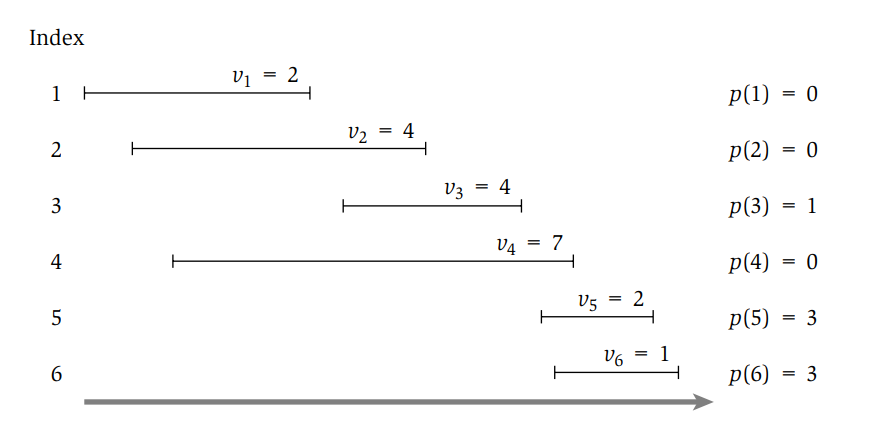
\includegraphics[width=12cm, keepaspectratio]{capitoli/imgs/weighted_problem.png}
    \caption{Istanza di un problema.}
\end{figure}

\section{Goal \normalfont{\emoji{soccer-ball}}}

L'obiettivo del nostro problema attuale è quello di trovare un sottoinsieme $S
    \subseteq \{1, \ldots, n\}$ di intervalli mutualmente compatibili che vanno a
massimizzare la somma dei pesi degli intervalli selezionati $\sum_{i \in S}
    v_i$.

\section{Funzionamento}

Come prima cosa definiamo il metodo per calcolare $OPT(j)$. Il problema è
una \textit{scelta binaria} che va a decidere se l'intervallo di indice $j$
verrà incluso nella soluzione oppure no basandosi sul valore ritornato dalla
seguente formula:

\begin{equation}
    \label{eqn:weight-opt}
    OPT(j) = max(v_j + OPT(p(j)), \ \ OPT(j-1))
\end{equation}
\ \\
Questo può essere anche visto come una disequazione:

\begin{equation}
    \label{eqn:weight-opt-dis}
    v_j + OPT(p(j)) \geq OPT(j-1)
\end{equation}
\ \\
che se vera, includerà $j$ nella soluzione ottimale.

\pagebreak

Scrivendo tutto sotto forma di algoritmo ricorsivo avremmo che:

\begin{lstlisting}[language=Javascript]
    function Compute-Opt(j){
        if (j == 0)
            return 0
        else
            return max(vj+Compute-Opt(p(j)), Compute-Opt(j − 1))
    }
\end{lstlisting}

Costruendo l'albero della ricorsione dell'algoritmo si nota che la complessità
temporale è esponenziale \emoji{astonished} !

\begin{figure}[H]
    \centering
    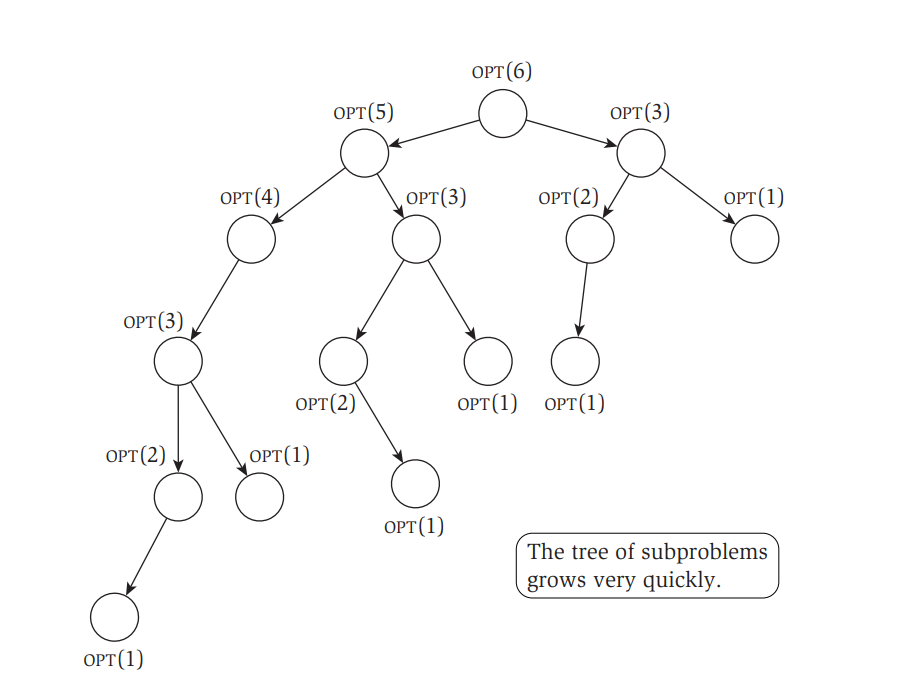
\includegraphics[width=12cm, keepaspectratio]{capitoli/imgs/opt_albero.png}
    \caption{Sviluppo dell'albero di ricorsione per la risoluzione di un problema.}
\end{figure}

\pagebreak

Una soluzione è quella di utilizzare la tecnica della \textbf{Memoization} che evita
di ricalcolare $OPT$ per gli indici già calcolati precedentemente, rendendo così
il costo temporale uguale ad $O(n)$ \emoji{man-in-motorized-wheelchair}.

\begin{lstlisting}[language=Javascript]
function M-Compute-Opt(j){
    if (j == 0)
        return 0
    else if (M[j] is not empty)
        return M[j]
    else
        let M[j] = max(vj+M-Compute-Opt(p(j)), M-Compute-Opt(j-1))
        return M[j]
}
\end{lstlisting}

Oltre al valore della soluzione ottimale probabilmente vorremmo sapere anche
quali sono gli intervalli che la compongono, e intuitivamente verrebbe da creare
un array aggiuntivo in cui verranno aggiunti gli indici degli intervalli
ottenuti con \verb|M-Compute-Opt|. Tuttavia questo aggiungerebbe una complessità
temporale di $O(n)$ peggiorando notevolmente le prestazioni. Un'alternativa è
quella di recuperare le soluzioni dai valori salvati nell'array \verb|M| dopo che la
soluzione ottimale è stata calcolata. Per farlo possiamo sfruttare la formula
vista in precedenza $v_j + OPT(p(j)) \geq OPT(j-1)$, che ci permette di
rintracciare gli intervalli della soluzione ottima.

\begin{lstlisting}[language=Javascript]
    function Find-Solution(j) {
        if (j == 0)
            Output nothing
        else if (vj + M[p(j)] >= M[j-1])
            Output j together with the result 
            of Find-Solution(p(j))
        else
            Output the result of Find-Solution(j-1)
    }
\end{lstlisting}
% \chapter{Least Squares Problem: Multi-way Choice \normalfont{\emoji{motorway}}}

Nel capitolo precedente l'algoritmo richiedeva una ricorsione basata su scelte
binarie, in questo capitolo invece introdurremo un algoritmo che richiede ad
ogni step un numero di scelte polinomiali (\textit{multi-way choice}). Vedremo
come la programmazione dinamica si presta molto bene a risolvere questi
problemi.

\section{Linear Least Square}

\subsection{Il Problema}

La formulazione del problema è la seguente:

\paragraph*{} dato un insieme $P$ composto di $n$ punti sul piano denotati con\\
$(x_1, y_1), (x_2, y_2), \ldots, (x_n, y_n)$; e supponiamo che $x_1 < x_2 <
    \ldots < x_n$ (sono strettamente crescenti). Data una linea $L$ definita
dall'equazione $y = ax + b$, definiamo l'\textit{errore} di $L$ in funzione
di $P$ come la somma delle distanze al quadrato della linea rispetto ai
punti in $P$. Formalmente:
\[
    Error(L, P) = \sum_{i=1}^{n} (y_i - ax_i - b)^2
\]

\begin{figure}[H]
    \centering
    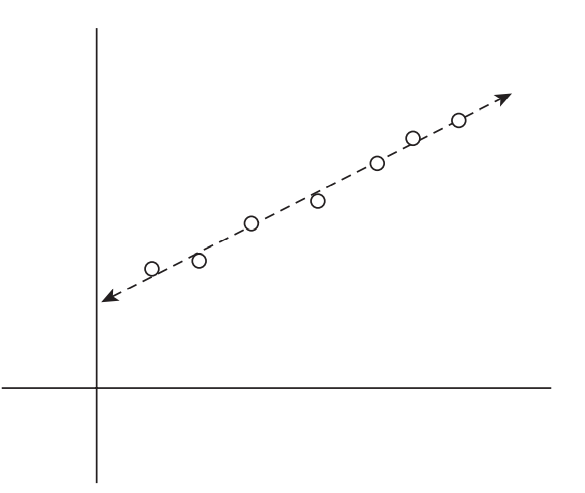
\includegraphics[width=6cm, keepaspectratio]{capitoli/imgs/linear_least.png}
    \caption{Esempio di una tipica istanza e soluzione del problema
        \textit{Linear Least}}
\end{figure}

\subsection{\goal}

È intuibile che il goal dell'algoritmo è quello di cercare la linea con errore
minimo, che può essere facilmente trovata utilizzando l'analisi matematica.
La linea di errore minimo è $y = ax + b$ dove:

\[
    a = \frac{n \sum_{i} x_i y_i - (\sum_{i} x_i) (\sum_{i} y_i)}{n \sum_{i} x_i^2 - (\sum_{i} x_i)^2} \ \ \  \ \ b = \frac{\sum_{i} y_i - a \sum_{i} x_i}{n}
\]

\section{Segmented Least Square}

Le formule appena citate sono utilizzabili solo se i punti di $P$ hanno un
andamento che è abbastanza lineare ma falliscono in altre circostanze.

\begin{figure}[H]
    \centering
    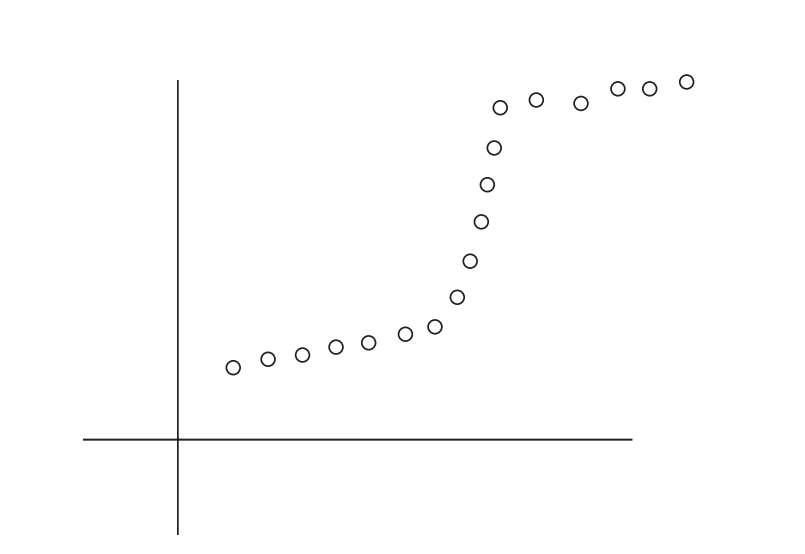
\includegraphics[width=8cm, keepaspectratio]{capitoli/imgs/segmente_linear_least.png}
    \caption{Esempio di funzione non risolvibile con Linear Least Square}
\end{figure}

Come è evidente (\textit{lapalissiano \normalfont{\emoji{gem}}}) dalla figura
non è possibile trovare una linea che approssimi in maniera soddisfacente i
punti, dunque per risolvere il problema possiamo pensare di rilassare la
condizione che sia solo una la linea. Questo però implica dover riformulare il
goal che altrimenti risulterebbe banale (si fanno $n$ linee che passano per ogni
punto).

\subsection{Costi}

La parte che computa gli errori ha costo in tempo $O(n^3)$ (si può portare a
$O(n^2)$).
La parte che trova il valore ottimo ha costo $O(n^2)$.\\

In spazio l'algoritmo ha costo $O(n^2)$ ma può essere ridotto a $O(n)$

\subsection{\goal}

Formalmente, il problema è espresso come segue:

\paragraph*{} come prima abbiamo un set di punti $P = \{(x_1, y_1), (x_2, y_2),
    \ldots, (x_n, y_n)\}$ strettamente crescenti. Denoteremo l'insieme dei punti
$(x_i, y_i)$ con $p_i$. Vogliamo partizionare $P$ in un qualche numero di
segmenti, ogni numero di segmenti è un sottoinsieme di $P$ che rappresenta un
\textit{set} contiguo delle coordinate $x$ con la forma $\{p_i, p_{i+1}, \ldots,
    p_{j-1}, p_j\}$ per degli indici $i \leq j$. Dopodiché, per ogni segmento $S$
calcoliamo la linea che minimizza l'errore rispetto ai punti in $S$ secondo
quanto espresso dalle formule enunciate prima.\\

Definiamo infine una penalità per una data partizione come la somma dei seguenti
termini:

\begin{itemize}
    \item Numero di segmenti in cui viene partizionato $P$ moltiplicato per un
          valore $C > 0$ (più è grande e più penalizza tante partizioni)
    \item Per ogni segmento l'errore della linea ottima attraverso quel
          segmento.
\end{itemize}


Il goal del Segmented Least Square Problem è quindi quello di trovare la
partizione di \textbf{penalità minima}.

\subsection{Funzionamento}

Per come è fatta la programmazione dinamica noi vogliamo suddividere il problema
in sotto-problemi e per farlo partiamo dall'osservazione che l'ultimo punto
appartiene ad una partizione ottima che parte da un valore $p_i$ fino a $p_n$ e
che possiamo togliere questi punti dal totale per ottenete un sotto-problema più
piccolo. Supponiamo che la soluzione ottima sia denotata da \verb|OPT(j)|, per i
punti che vanno da $p_1$ a $p_j$, allora avremo che la soluzione ottima al
problema dato l'ultimo segmento che va da $p_i$ a $p_n$, sarà dalla seguente
formula:

\[
    OPT(n) = e_{i,n} + C + OPT(i - 1)
\]

Questa formula è data dalla soluzione ottima dell'ultima partizione ($e_{i,n} + C$)
a cui viene aggiunta la soluzione ottima di tutte le partizioni precedenti
($OPT(i -1)$). Per i sotto-problemi possiamo scrivere la soluzione al problema
in forma ricorsiva utilizzando la formula appena espressa che prenderà la forma:

\[
    OPT(j) = \min_{1 \leq i \leq j}(e_{i,j} + C + OPT(i - 1))
\]

Possiamo ora dare una versione di questo algoritmo in pseudocodice:

\begin{lstlisting}[language=Javascript]
    function Segmented-Least-Squares(n) {
        M[0 ... n]
        M[0] = 0

        // compute the errors
        for (j in 1 ... n) {
            for (i in 1 ... j) {
                compute eij for the segment pi, ..., pj
            }
        }

        // find optimal value
        for (j in 1 ... n) {
            M[j] = min_i(eij + C + M[i - 1]) // OPT(J)
        }

        return M[n]
    }
\end{lstlisting}

Dopo aver trovato la soluzione ottima, possiamo sfruttare la memoization per
ricavarci i segmenti in tempi brevi.

\begin{lstlisting}[language=Javascript]
    function Find-Segments(j) {
        if (j == 0) print('')

        else {
            Find an i that minimizes ei,j + C + M[i − 1]
            Output the segment {pi,..., pj} and the result of Find-Segments(i − 1)
        }
    }
\end{lstlisting}

L'algoritmo ha costo $O(n^3)$ in tempo e $O(n^2)$ in spazio.
Questo tempo può essere ridotto applicando la memoization alle formule per il calcolo
dell'errore viste in precedenza portandolo a $O(n^2)$ per il tempo e $O(n)$ per lo spazio.
% \chapter{Subset Sum \& Knapsack Problem \normalfont{\emoji{money-bag}}}

\section{Il Problema}

Il problema delle Subset Sum è formalmente definito come segue:\\

\- abbiamo $n$ oggetti $\{1, \ldots, n\}$, a ognuno viene assegnato un
peso non negativo $w_i$ (per $i = 1, \ldots, n$) e ci viene dato anche un
limite $W$. L'obbiettivo è quello di selezionare un sottoinsieme $S$ degli
oggetti tale che $\sum_{i \in S}w_i \leq W$ e che questa sommatoria abbia valore
più grande possibile.\\

Questo problema è un caso specifico di un problema più generale conosciuto come
il Knapsack Problem, l'unica differenza sta nel valore da massimizzare che per il
Knapsack è un valore $v_i$ e non più il peso.

Si potrebbe pensare di risolvere questi problemi con un algoritmo greedy ma
purtroppo non ne esiste uno in grado di trovare efficientemente la soluzione ottima.
Potremmo pensare di ordinare gli oggetti in base al peso in ordine crescente o
decrescente e prenderli, tuttavia questo approccio fallisce per determinati casi
(come per l'insieme $\{W/2+1, W/2, W/2\}$ ordinato in senso decrescente) e l'unica
opzione sarà quella di provare con la programmazione dinamica \emoji{person-in-manual-wheelchair}.
\newpage

\section{\goal}

Possiamo riassumere il goal di questi problemi come segue:\\

\- Abbiamo $n$ oggetti $\{1, \ldots, n\}$, a ognuno viene assegnato un
peso non negativo $w_i$ (per $i = 1, \ldots, n$) e ci viene dato anche un
limite $W$. L'obbiettivo è quello di selezionare un sottoinsieme $S$ degli oggetti
tale che $\sum_{i \in S}w_i \leq W$ e che questa sommatoria abbia valore più
grande possibile.

\section{Costi}

\begin{center}
    \begin{tabular}{|c|c|}
        \centering
        \textbf{Funzione}    & \textbf{Costo (tempo)} \\
        \verb|Subset-Sum|    & $O(nW)$                \\
        \verb|Find-Solution| & $O(n)$                 \\
    \end{tabular}
\end{center}

\section{Funzionamento}

Come per tutti gli algoritmi dinamici dobbiamo cercare dei sotto-problemi e
possiamo utilizzare la stessa intuizione avuto per il problema dello scheduling
(scelta binaria). Facendo tutti i calcoli di dovere otteniamo la seguente
ricorsione:

\begin{center}
    se $w < w_i$ allora $OPT(i, w) = OPT(i-1,w)$ altrimenti\\
    $OPT(i, w) = max(OPT(i-1, w), w_i + OPT(i-1, w-w_i))$
\end{center}

Nella prima parte analizziamo il caso in cui l'elemento che vogliamo aggiungere va
a superare il peso massimo residuo $w$, dunque viene scartato. Nella seconda parte
andiamo ad analizzare se l'aggiunta o meno del nuovo oggetto va a migliorare
la soluzione di $OPT$ che è definita come:\\

\[
    OPT(i, w) = \max_{S} \sum_{j \in S} w_j
\]
\newpage

Possiamo formalizzare il tutto con il seguente pseudo-codice:

\begin{lstlisting}[language=JavaScript]
    function Subset-Sum(n, W) {
        let M[0 . . . n,0... W]

        //initialize the memoization vector
        for(w in 0 ... W) {
            M[0, W] = 0
        }

        //solve subproblems
        for(i in 1 ... n) {
            for(w in 0 ... W) {
                Use the recurrence to compute M[i, w]
            }
        }

        return M[n, W]
    }
\end{lstlisting}

La particolarità di questo algoritmo è che avremmo 2 insiemi di sotto-problemi
diversi che devono essere risolti per ottenere la soluzione ottima. Questo fatto
si riflette in come viene popolato l'array di memoization dei valori di $OPT$
che verranno salvati in un array bidimensionale.

\begin{figure}[H]
    \centering
    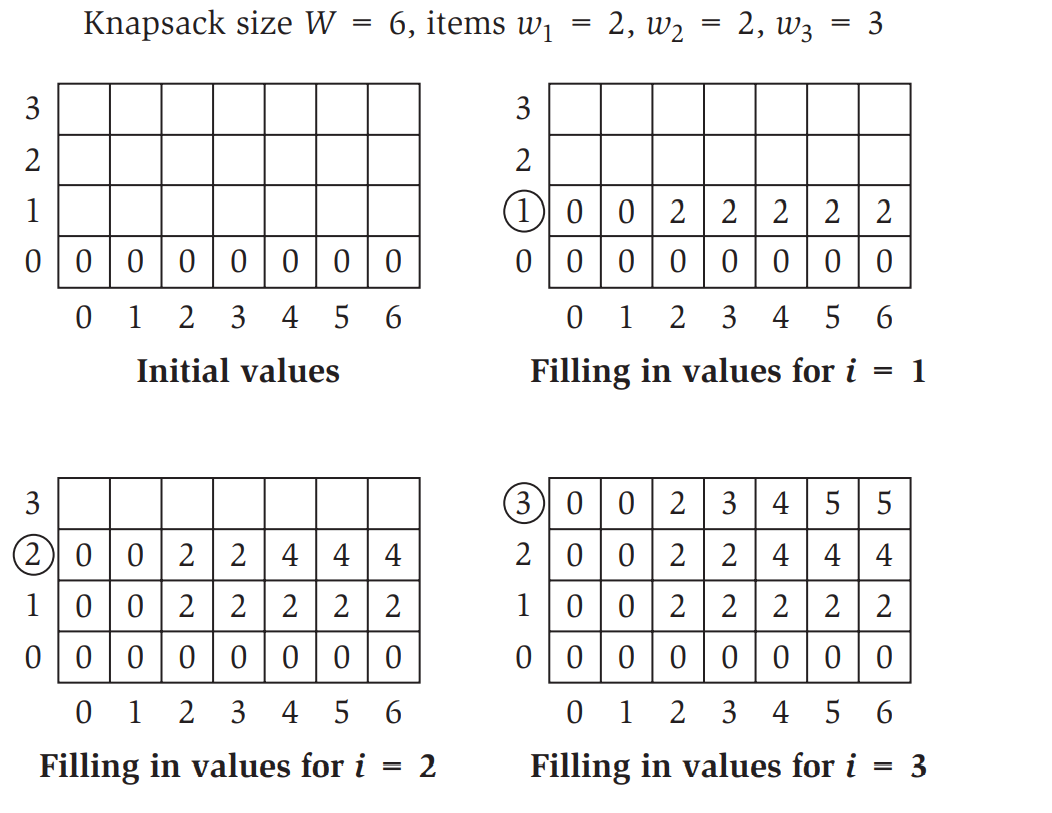
\includegraphics[width=10cm, keepaspectratio]{capitoli/imgs/knapsac_table.png}
    \caption{Esempio di come viene popolato l'array $M$ per il problema del Knapsack.}
\end{figure}

\textit{Il costo in tempo di questa implementazione è di $O(nW)$.}\\

A causa di questo costo, l'algoritmo fa parte della famiglia degli
algoritmi \textit{pseudo polinomiali}, ovvero algoritmi il cui costi dipende da
una variabile di input che se piccola, lo mantiene basso e se grande lo fa
esplodere.\\

\textit{Per recuperare gli oggetti dall'array di Memoization la complessità in tempo è di
    $O(n)$.}\\

Questa implementazione funziona anche per il problema più generale del Knapsack,
ci basterà solo cambiare la parte di ricorsione scrivendola come segue:

\begin{center}
    se $w < w_i$ allora $OPT(i, w) = OPT(i-1,w)$ altrimenti
    $OPT(i, w) = max(OPT(i-1, w), v_i + OPT(i-1, w-w_i))$
\end{center}

La complessità temporale è sempre $O(nW)$.
% \section{RNA Secondary Structure \normalfont{\emoji{dna}}}

La ricerca della struttura secondaria dell'RNA è un problema a 2 variabili
risolvibile tramite il paradigma della programmazione dinamica. Come sappiamo il
DNA è composto da due filamenti, mentre l'RNA è composto da un filamento
singolo. Questo comporta che spesso le basi di un singolo filamento di RNA si
accoppino tra di loro. L'insieme della basi può essere visto come l'alfabeto
$\{A, C, U, G\}$ e l'RNA è una sequenza di simboli presi da questo alfabeto. Il
processo di accoppiamento delle basi è dettato dalla regola di \textit{Watson-Crick} e
segue il seguente schema:

\[
    A - U \ \ \ \textrm{ e } \ \ \ C - G \ \ \ \textrm{ (l'ordine non conta)}
\]

\begin{figure}[H]
    \centering
    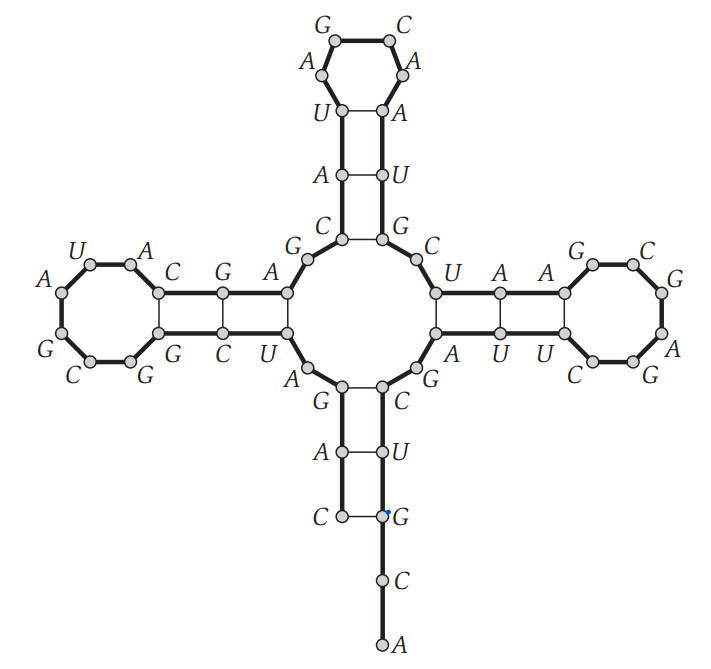
\includegraphics[width=8cm, keepaspectratio]{capitoli/dynamic_programming/imgs/rna_esempio1.png}
    \caption{Esempio di una struttura secondari di RNA} %%TODO: ricontrollare !!
\end{figure}

\subsection{Il Problema}

In questo problema si vuole trovare la struttura secondaria dell'RNA che abbia
energia libera maggiore (il maggior numero di coppie di basi possibili). Per
farlo dobbiamo tenere in considerazione alcune condizioni che devono essere
soddisfatte per permettere di approssimare al meglio il modello biologico
dell'RNA.\\

Formalmente la struttura secondaria di $B$ è un insieme di coppie $S =
    \{(i,j)\}$ dove $i,j \in \{1,2,\ldots,n\}$, che soddisfa le seguenti
condizioni:

\begin{enumerate}
    \item \textbf{No Sharp Turns}: la fine di ogni coppia è separata da almeno 4
          basi, quindi se $(i,j) \in S$ allora $i < j - 4$
    \item Gli elementi di una qualsiasi coppia $S$ consistono di $\{A, U\}$ o
          $\{C, G\}$ (in qualsiasi ordine).
    \item $S$ è un \textit{matching}: nessuna base compare in più di una coppia.
    \item \textbf{Non Crossing Condition}: se $(i, j)$ e $(k,l)$ sono due coppie
          in $S$ allora \textbf{non} può avvenire che $i < k < j < l$.
\end{enumerate}

\begin{figure}[H]
    \centering
    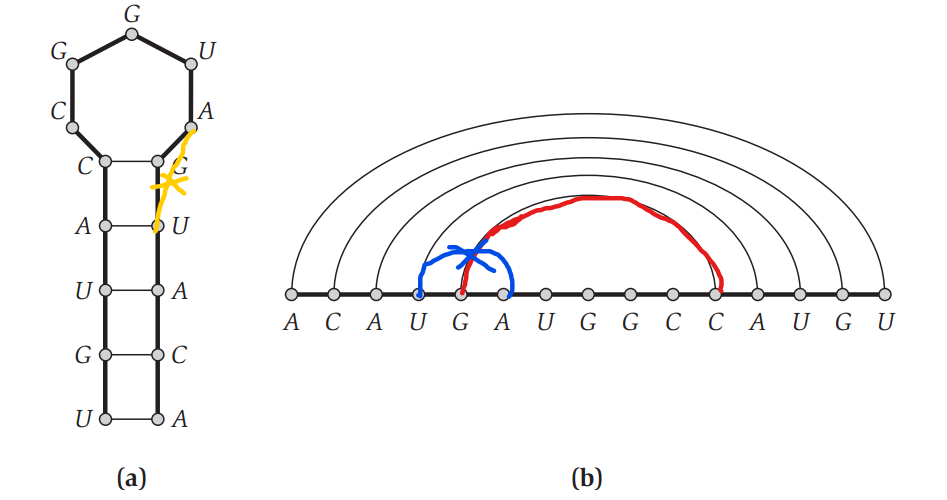
\includegraphics[width=10cm, keepaspectratio]{capitoli/dynamic_programming/imgs/rna_esempio2.png}
    \caption{La figura \textit{(a)} rappresenta un esempio di \textit{Sharp
            Turn}, mentre la figura \textit{(b)} mostra una
        \textit{Crossing Condition} dove il filo blu non dovrebbe esistere.}
\end{figure}

\subsection{\goal}

Il goal di questo problema è di massimizzare la quantità di coppie che si possono
formare all'interno della struttura secondaria di una data sequenza di RNA.

\subsection{Costi}

L'algoritmo complessivo ha costo $O(n^3)$.

\subsection{Funzionamento}

\paragraph{First Attempt.}
Come primo tentativo potremmo basarci sul seguente sotto-problema: affermiamo che
$OPT(j)$ è il massimo numero di coppie di basi sulla struttura secondaria $b_1
    b_2 \ldots b_j$, per la Non Sharp Turn Condition sappiamo che $OPT(j) = 0$ per
$j \leq 5$ e sappiamo anche che $OPT(n)$ è la soluzione che vogliamo trovare. Il
problema ora sta nell'esprimere $OPT(j)$ ricorsivamente. Possiamo parzialmente
farlo sfruttando le seguenti scelte:

\begin{itemize}
    \item $j$ non appartiene ad una coppia
    \item $j$ si accoppia con $t$ per qualche $t \leq
              j - 4$
\end{itemize}

Per il primo caso basta cercare la soluzione per $OPT(j - 1)$, nel secondo caso
invece se teniamo conto della Non Crossing Condition, possiamo isolare due nuovi
sotto-problemi: uno sulle basi $b_1 b_2 \ldots b_{t-1}$ e l'altro sulle basi
$b_{t+1} \ldots b_{j-1}$. Il primo si risolve con $OPT(t-1)$ ma il secondo, dato
che non inizia con indice $1$, non è nella lista dei nostri sotto-problemi. A
causa di ciò risulta necessario aggiungere una variabile.

\begin{figure}[H]
    \centering
    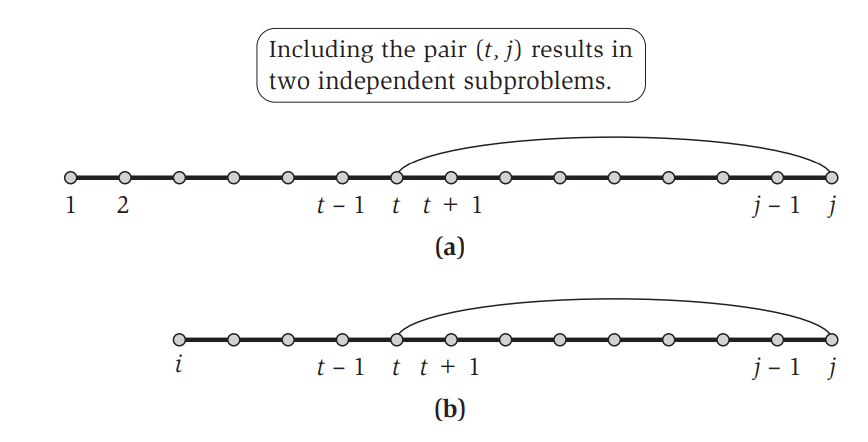
\includegraphics[width=10cm, keepaspectratio]{capitoli/dynamic_programming/imgs/rna_funzionamento.png}
    \caption{Esempio di
        utilizzo di una sola variabile \textit{(a)} o con due \textit{(b)}.}
\end{figure}

\paragraph{Dynamic Programming over Intervals}
Basandoci sui ragionamenti precedenti, possiamo scrivere una ricorsione di
successo: sia $OPT(i,j)$ il numero massimo di coppie di basi nella struttura
secondaria $b_i b_{i+1} \ldots b_j$, grazie alla non sharp turn Condition
possiamo inizializzare gli elementi con $i \geq j -4$ a $0$. Ora avremmo sempre
le stesse condizioni elencate sopra:

\begin{itemize}
    \item $j$ non appartiene ad una coppia
    \item $j$ si accoppia con $t$ per qualche $t \leq j - 4$
\end{itemize}

Nel primo caso avremmo che $OPT(i,j) = OPT(i, j-1)$, nel secondo caso possiamo
ricorrere su due sotto-problemi $OPT(i, t-1)$ e $OPT(t+1, j-1)$ affinché venga
rispettata la non crossing condition. Possiamo esprimere formalmente la
ricorsione come segue:

\begin{center}
    \[
        OPT(i, j) = \max(OPT(i, j-1), \max_t(1+OPT(i, t-1)+OPT(t+1, j-1))),
    \]
    dove il massimo è calcolato su $t$ tale che $b_t$ e $b_j$ siano una coppia di
    basi consentita
\end{center}

\begin{figure}[H]
    \centering
    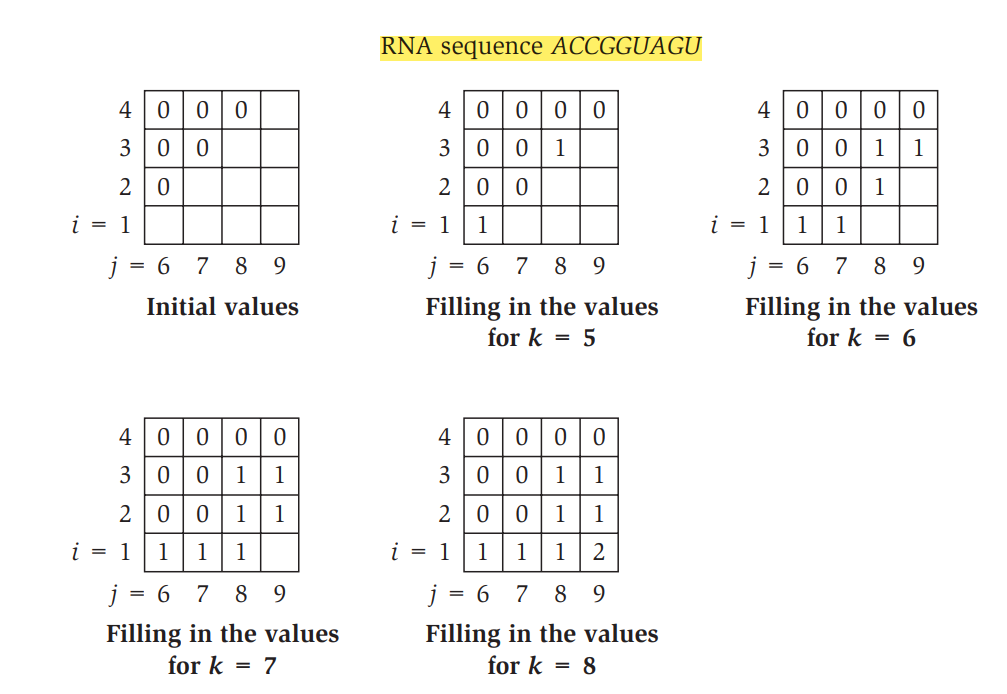
\includegraphics[width=\textwidth, keepaspectratio]{capitoli/dynamic_programming/imgs/rna_calcolo.png}
    \caption{Iterazioni dell'algoritmo su un campione del problema in questione $ACCGGUAGU$}
\end{figure}
\newpage

Possiamo infine formalizzare il tutto con il seguente pseudo-codice:

\begin{lstlisting}[language=JavaScript]
 Initialize OPT(i, j) = 0 whenever i ≥ j - 4

 for (k in 5 ... n - 1) {
     for (i in 1 ... n - k) {
         j = i + k
         Compute OPT(i, j) using the previous recurrence
     }
 }

 return OPT(1, n)
\end{lstlisting}

Ci sono $O(n^2)$ sotto-problemi da risolvere e ognuno richiede tempo $O(n)$,
quindi il running time complessivo è di $O(n^3)$.

% \section{Sequence Alignment}

Il problema del Sequence Alignment consiste nel riuscire a comparare delle
stringhe, come per esempio quando si effettua un typo in un motore di ricerca e
quello ci fornisce l'alternativa corretta. Una prima idea potrebbe essere quella
di \textbf{allineare} le due parole lettera per lettera, riempendo gli eventuali
spazi bianchi, e vedendo di quanto le due differiscono. Tuttavia ci sono varie
possibilità con cui due parole di lunghezza diversa possono essere confrontate,
quindi è necessario fornire una definizione di \textbf{similarità}.

\subsection{Il Problema}

Come prima definizione di similarità possiamo dire che minore sarà il numero di
caratteri che non corrispondono, maggiore sarà la similarità tra le parole.
Questa problematica è anche un tema centrale della biologia molecolare, e
proprio grazie ad un biologo abbiamo una definizione rigorosa e soddisfacente di
similarità. Prima di dare una definizione similarità dovremo però darne una di
\textbf{allineamento}: Supponiamo di avere due stringhe $X$ e $Y$, che consistono rispettivamente
della sequenza di simboli $x_1 x_2 \ldots x_m$ e $y_1 y_2 \ldots y_n$, e
consideriamo gli insiemi $\{1,2,\ldots ,m\}$ e $\{1,2,\ldots ,n\}$ che
rappresentano le varie posizioni nelle stringhe $X$ e $Y$, ora si considera un
\textbf{Matching} di queste due parole (un matching è stato definito nella parte
precedente e si tratta di un insieme di coppie ordinate con la proprietà che
ogni oggetto si trova al più in una sola coppia).  Diciamo ora che un matching
$M$ di questi due insiemi è un allineamento se gli elementi di varie coppie non
si incrociano: se $(i,j),(i^{\prime},j^{\prime}) \in M$  e $i < i^{\prime}$,
allora $j < j^{\prime}$.\\

Ora la nostra definizione di similarità si baserà sul trovare il miglior
allineamento, seguendo i seguenti criteri:

\begin{itemize}
    \item C'è un parametro $\delta>0$ che
          definisce la \textbf{gap penalty}, ovvero ogni volta che un simbolo di una parola
          non corrisponde ad un simbolo dell'altra.
    \item Per ogni coppia di lettere $p,q$ del
          nostro alfabeto, se c'è un accoppiamento errato si paga il corrispondente
          \textbf{mismatch cost} $a_(p,q)$.
    \item Il costo di $M$ è la somma del suo gap e mismatch
          cost, e l'obiettivo sarà quello di minimizzarlo.
\end{itemize}

\subsection{Creazione dell'algoritmo}

Ora affronteremo il problema di calcolarci questo costo minimo, e l'allineamento
ottimale che lo fornisce date le coppie $X$ e $Y$. Come al solito proveremo con
un approccio di programmazione dinamica, e per realizzare l'algoritmo
individuiamo come per altri algoritmi già visti una scelta binaria. Dato
l'allineamento ottimale $M$ allora:

\begin{itemize}
    \item $(m,n) \in M$ (quindi gli ultimi due
          simboli delle 2 stringhe sono in un matching)
    \item $(m,n) \notin M$ (gli ultimi
          simboli delle due stringhe non sono in un matching)
\end{itemize}

Tuttavia questa semplice distinzione non è sufficiente, quindi supponiamo di
aggiungere anche il seguente fatto elementare:\\

\- Sia $M$ un qualsiasi allineamento di $X$ e $Y$. se $(m,n) \notin M$, allora o
l' $m-esima$ posizione di $X$ o l' $n-esima$ posizione di $Y$ non è in un
matching di $M$.\\

Dire questo equivale a riscrivere le due condizioni sopra come tre, dunque in un
allineamento ottimo $M$ almeno una deve essere vera:

\begin{itemize}
    \item $(m,n) \in M$
    \item l'$m-esima$ posizione di $X$ non è nel matching
    \item l' $n-esima$ posizione di $Y$ non è nel matching
\end{itemize}

Ora definiamo la funzione di costo minimo $OPT(i,j)$ come costo dell'alignmet
tra $x_1 x_2 \ldots x_i$ e $y_1 y_2 \ldots y_j$. In base alle condizioni
espresse in precedenza la funzione $OPT(m,n)$ assumerà il costo relativo più
$OPT(m-1,n-1)$, in particolare (i tre casi citati sopra):

\begin{itemize}
    \item condizione 1, si
          paga un matching cost per le lettere $m,n$
    \item condizione 2 e 3, si paga un gap
          cost $\delta$ per $m$(condizione 2) o $n$(condizione 3)
\end{itemize}

Utilizzando dunque gli stessi argomenti per per i sotto problemi per
l'allineamento di costo minimo tra $X$ e $Y$ otteniamo la definizione generale
di $OPT(i,j)$:\\

L'allineamento di costo minimo soddisfa la seguente ricorsione per $i \geq 1$
e $j \geq 1$:
\[
    OPT(i,j) = min[a_{(x_i y_j)} + OPT(i-1, j-1),
            \delta + OPT(i-1, j), \delta + OPT(i, j-1)]
\]

Dunque così abbiamo ottenuto la nostra funzione di ricorsione e possiamo
procedere alla scrittura dello pseudo codice.

\begin{lstlisting}[language=JavaScript]
    function alignment(X,Y) { var A = Matrix(m, n)

        Initialize A[i, 0]= iδ for each i 
        Initialize A[0, j]= jδ for each j

        for (j in 1...n) { 
            for (i in 1...m) { 
                Use the recurrence (6.16) to compute A[i, j] 
            }
        }

        return A[m, n]
    }
\end{lstlisting}

Il running time è di $O(mn)$

\subsection{Sequence Alignment in Spazio Lineare}

Come abbiamo appena visto l'algoritmo ha sia costo spaziale che temporale uguale
a $O(mn)$ e se come input consideriamo le parole della lingua inglese non
risulta essere un grande problema, ma se consideriamo genomi con 10 miliardi di
caratteri potrebbe risultare difficile poter lavorare con array di 10 GB \emoji{astonished}.
Questo problema può essere risolto utilizzando un approccio \textit{divide et impera}
che va a rendere lineare il costo dello spazio ( $O(n + m)$ ).

\subsubsection{Funzionamento}

Come prima cosa definiamo un algoritmo Space Efficient Alignment che ci permette
di trovare la soluzione ottima utilizzando il minor spazio possibile. Per farlo
notiamo che la funzione $OPT$ dipende solamente da una colonna precedente di
quella che si sta analizzando, dunque basterà caricarsi in memoria una matrice
$mx2$ riducendo così il costo spaziale ad $m$. Tuttavia utilizzando questo
metodo non e possibile ricurvare l'alignment effettivo perché non ci bastano le
informazioni.\\

Lo pseudo-codice dell'algoritmo appena definito è il seguente:

\begin{lstlisting}[language=JavaScript]
    function Space-Efficient-Alignment(X,Y) {
        var B = Matrix(m, 2)

        // (just as in column 0 of A)
        Initialize B[i, 0]= iδ for each i 

        for (j in 1...n) {
            B[0, 1]= jδ (since this corresponds to entry A[0, j])

            for (i in 1...m) {
                B[i, 1]= min[
                    αxiyj + B[i − 1, 0],
                    δ + B[i − 1, 1], 
                    δ + B[i, 0]
                ]
            }

            Move column 1 of B to column 0 to make room 
            for next iteration:
            Update B[i, 0] = B[i, 1] for each i
        }
    }
\end{lstlisting}

Possiamo quindi utilizzare un approccio \textit{divide et impera} che incorpora 2
tecniche diverse di programmazione dinamica per sfruttare questo approccio
appena definito e riuscire a trovare anche l'alignment in spazio lineare.
Definiamo quindi due funzioni:

\begin{itemize}
    \item $f(i, j)$ : è la funzione definita per l'algoritmo di Sequence
          Alignment di base (analoga a $OPT(i,j)$ )
    \item $g(i, j)$ : è l'analogo al contrario di $f$ ed è definito dalla
          seguente funzione ricorsiva: per $i < m$ e $j < n$ : $g(i,j) =
              min[a_{x+1y+1} + g(i+1, j+1), \delta + g(i, j+1), \delta + g(i+1, j)]$
\end{itemize}

Possiamo notare che la ricorsione $f$ procede a ritroso partendo dal fondo
mentre la ricorsione $g$ procede in avanti partendo dall'inizio. Possiamo
sfruttare questo fatto per provare ad utilizzare lo Space Efficiente Sequence
Alignment Algorithm combinato ad un approccio \textit{divide et impera} e un array di
supporto $P$ per riuscire a calcolare il Sequence Alignment in spazio lineare,
aumentando solo di una costatane la complessità temporale.\\

Possiamo riassumere il tutto con il seguente pseudo-codice:

\begin{lstlisting}[language=JavaScript]
    function Divide-and-Conquer-Alignment(X,Y) {
        var m = length(X)
        var n = length(Y)

        if (m <= 2 or n <= 2) {
            Compute optimal alignment using Alignment(X,Y)
        }

        Space-Efficient-Alignment(X, Y[1 : n/2])
        Backward-Space-Efficient-Alignment(X, Y[n/2 + 1 : n])

        Let q be the index minimizing f(q, n/2) + g(q, n/2)
        Add (q, n/2) to global list P

        Divide-and-Conquer-Alignment(X[1 : q],Y[1 : n/2])
        Divide-and-Conquer-Alignment(X[q + 1 : n],Y[n/2 + 1:n])

        return P
    }
\end{lstlisting}

\begin{figure}[H]
    \centering
    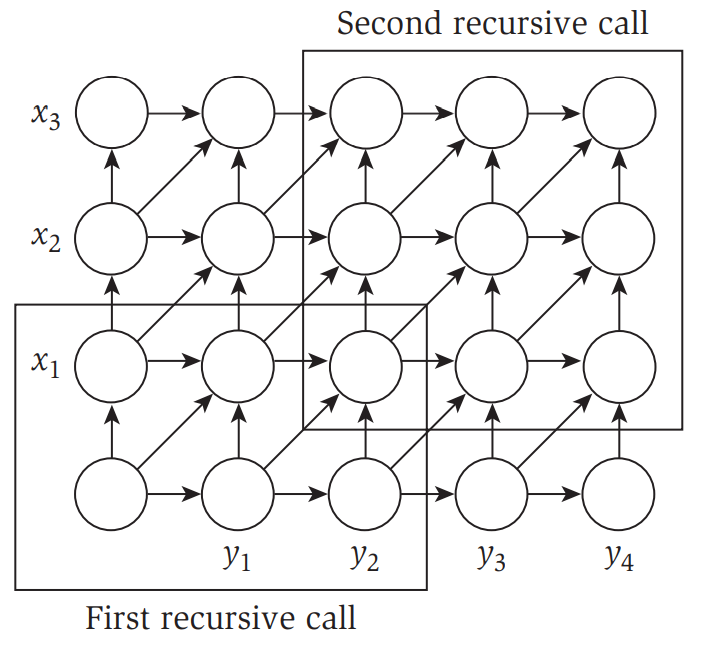
\includegraphics[width=8cm, keepaspectratio]{capitoli/dynamic_programming/imgs/seq_align_recurrence.png}
    \caption{La figura mostra il funzionamento dell'algoritmo appena descritto.}
\end{figure}

\documentclass[a4paper,12 pt]{report}
\usepackage[T1]{fontenc}
\usepackage[utf8]{inputenc}
% \usepackage{amsmath}
\usepackage{lmodern}
\usepackage{listings}
\usepackage{graphicx}
\usepackage{float}
\usepackage{subcaption}
\usepackage{hyperref}
\usepackage{wrapfig}
\usepackage{fancyhdr}
% \usepackage{tcolorbox}

% forza le footnote a stare il più in basso possibile
\usepackage[bottom]{footmisc}
\usepackage{enumitem}

%% STILE LISTINGS

\usepackage{xcolor}

\definecolor{codegreen}{rgb}{0,0.6,0}
\definecolor{codegray}{rgb}{0.5,0.5,0.5}
\definecolor{codepurple}{rgb}{0.58,0,0.82}
\definecolor{backcolour}{rgb}{0.95,0.95,0.92}

\lstdefinestyle{mystyle}{
    backgroundcolor=\color{backcolour},   
    commentstyle=\color{codegreen},
    keywordstyle=\color{magenta},
    numberstyle=\tiny\color{codegray},
    stringstyle=\color{codepurple},
    basicstyle=\ttfamily\footnotesize,
    breakatwhitespace=false,         
    breaklines=true,                 
    captionpos=b,                    
    keepspaces=true,                 
    numbers=left,                    
    numbersep=5pt,                  
    showspaces=false,                
    showstringspaces=false,
    showtabs=false,                  
    tabsize=2
}

\lstset{style=mystyle}

%% SOLIDITY Settings

% Copyright 2017 Sergei Tikhomirov, MIT License
% https://github.com/s-tikhomirov/solidity-latex-highlighting/

%\usepackage{listings, xcolor}

\definecolor{verylightgray}{rgb}{.97,.97,.97}

\lstdefinelanguage{Solidity}{
	keywords=[1]{anonymous, assembly, assert, balance, break, call, callcode, case, catch, class, constant, continue, constructor, contract, debugger, default, delegatecall, delete, do, else, emit, event, experimental, export, external, false, finally, for, function, gas, if, implements, import, in, indexed, instanceof, interface, internal, is, length, library, log0, log1, log2, log3, log4, memory, modifier, new, payable, pragma, private, protected, public, pure, push, require, return, returns, revert, selfdestruct, send, solidity, storage, struct, suicide, super, switch, then, this, throw, transfer, true, try, typeof, using, value, view, while, with, addmod, ecrecover, keccak256, mulmod, ripemd160, sha256, sha3}, % generic keywords including crypto operations
	keywordstyle=[1]\color{blue}\bfseries,
	keywords=[2]{address, bool, byte, bytes, bytes1, bytes2, bytes3, bytes4, bytes5, bytes6, bytes7, bytes8, bytes9, bytes10, bytes11, bytes12, bytes13, bytes14, bytes15, bytes16, bytes17, bytes18, bytes19, bytes20, bytes21, bytes22, bytes23, bytes24, bytes25, bytes26, bytes27, bytes28, bytes29, bytes30, bytes31, bytes32, enum, int, int8, int16, int24, int32, int40, int48, int56, int64, int72, int80, int88, int96, int104, int112, int120, int128, int136, int144, int152, int160, int168, int176, int184, int192, int200, int208, int216, int224, int232, int240, int248, int256, mapping, string, uint, uint8, uint16, uint24, uint32, uint40, uint48, uint56, uint64, uint72, uint80, uint88, uint96, uint104, uint112, uint120, uint128, uint136, uint144, uint152, uint160, uint168, uint176, uint184, uint192, uint200, uint208, uint216, uint224, uint232, uint240, uint248, uint256, var, void, ether, finney, szabo, wei, days, hours, minutes, seconds, weeks, years},	% types; money and time units
	keywordstyle=[2]\color{teal}\bfseries,
	keywords=[3]{block, blockhash, coinbase, difficulty, gaslimit, number, timestamp, msg, data, gas, sender, sig, value, now, tx, gasprice, origin},	% environment variables
	keywordstyle=[3]\color{violet}\bfseries,
	identifierstyle=\color{black},
	sensitive=false,
	comment=[l]{//},
	morecomment=[s]{/*}{*/},
	commentstyle=\color{gray}\ttfamily,
	stringstyle=\color{red}\ttfamily,
	morestring=[b]',
	morestring=[b]"
}

\lstdefinelanguage{JavaScript}{
  keywords={typeof, new, true, false, catch, function, return, null, catch, switch, var, if, in, while, do, else, case, break},
  keywordstyle=\color{blue}\bfseries,
  ndkeywords={class, export, boolean, throw, implements, import, this},
  ndkeywordstyle=\color{darkgray}\bfseries,
  identifierstyle=\color{black},
  sensitive=false,
  comment=[l]{//},
  morecomment=[s]{/*}{*/},
  commentstyle=\color{purple}\ttfamily,
  stringstyle=\color{red}\ttfamily,
  morestring=[b]',
  morestring=[b]"
}
%\lstset{
%	language=Solidity,
%	backgroundcolor=\color{verylightgray},
%	extendedchars=true,
%	basicstyle=\footnotesize\ttfamily,
%	showstringspaces=false,
%	showspaces=false,
%	numbers=left,
%	numberstyle=\footnotesize,
%	numbersep=9pt,
%	tabsize=2,
%	breaklines=true,
%	showtabs=false,
%	captionpos=b
%}

%% -----

% box around text
\newenvironment{boxed}
    {\begin{center}
    \begin{tabular}{|p{\textwidth}|}
    \hline\\
    }
    { 
    \\\\\hline
    \end{tabular} 
    \end{center}
    }

% Resetta la numerazione dei chapter quando
% una nuova part viene creata
\makeatletter
\@addtoreset{chapter}{part}
\makeatother

% Rimuove l'indentazione quando si crea un nuovo paragrafo
\setlength{\parindent}{0pt}

% footer
\pagestyle{fancyplain}
% rimuove la riga nell'header
\fancyhf{} % sets both header and footer to nothing
\renewcommand{\headrulewidth}{0pt}
\fancyfoot[L]{\href{https://github.com/Typing-Monkeys/AppuntiUniversita}{Typing Monkeys}}
\fancyfoot[C]{\emoji{gorilla}}
\fancyfoot[R]{\thepage}

% configurazione emoji
\usepackage{fontspec}
\usepackage{emoji}
\setemojifont{NotoColorEmoji.ttf}[Path=/usr/share/fonts/truetype/noto/]


% Macro
\newcommand{\goal}{Goal \normalfont{\emoji{soccer-ball}}}


\begin{document}
\include{frontmatter/main.tex}

%% TODO: riorganizzare la struttura degli appunti
%%       alla fine dovremmo avere una roba del tipo
%%          - Programmazione Dinamica
%%            - Arg 1
%%            - Arg 2
%%              - subarg 1
%%              - subarg 2
%%          - Flow
%%            - Arg 1
%%              - sub arg 1
%%          - Graph
%%            - Arg 1
%%

\tableofcontents

\include{quote/main.tex}

% \include{capitoli/dynamic_programming/1-introduzione_all_programmazione_dinamica.tex}
% \include{capitoli/dynamic_programming/2-weighted_interval_scheduling.tex}
% \include{capitoli/dynamic_programming/3-least_squares_problem_multiway_choice.tex}
% \include{capitoli/dynamic_programming/4-subset_sum_e_knapsack_problem.tex}
% \include{capitoli/dynamic_programming/5-rna_secondary_structure.tex}
% \include{capitoli/dynamic_programming/6-sequence_alignment.tex}
\include{capitoli/dynamic_programming/main.tex}

\end{document}

\end{document}

% \section{Introduzione alla Programmazione Dinamica}

Dopo aver visto tecniche di design degli algoritmi quali Greedy e Divide et
Impera, è importante introdurre una tecnica più potente ma anche più complessa
da applicare: la Programmazione Dinamica (Dynamic Programming).\\

Prima di analizzarla in modo approfondito, spiegheremo a grandi linee il suo
funzionamento. L'idea di base si fonda sulla tecnica Divide et Impera ed è
essenzialmente l'opposto di una strategia Greedy, in sostanza si esplora
implicitamente tutto lo spazio delle soluzioni e si decompone in una serie di
sotto-problemi, grazie ai quali si costruiscono soluzioni corrette per
sotto-problemi sempre più grandi finché non si raggiunge il problema di
partenza.\\
\- Una tecnica di programmazione dinamica è quella della memoization che è utile
per risolvere una moltitudine di problemi e per applicare la programmazione
dinamica è necessario creare un sotto-set di problemi che soddisfano le seguenti
proprietà:

\begin{enumerate}
      \item Esistono solo un numero polinomiale di sotto-problemi
      \item La soluzione al
            problema originale può essere calcolata facilmente dalla soluzione dei
            sotto-problemi
      \item C'è un ordinamento naturale dei sotto-problemi dal più piccolo
            al più grande, insieme a una ricorsione facilmente calcolabile
\end{enumerate}

% \chapter{Weighted Interval Scheduling\normalfont{\emoji{man-lifting-weights}}}

Questo algoritmo cerca di ottenere un insieme di intervalli non sovrapposti
(\textit{overlapping}) che è il più grande possibile. Per la versione senza pesi
($weight = 1$) esiste uno specifico algoritmo greedy che è in grado di trovare la
soluzione ottima, tuttavia nella versione pesata ($weight \neq 1$) sarà
necessario utilizzare la programmazione dinamica.

\section{Costi}

%% TODO: migliorare sta tabella
\begin{center}
    \begin{tabular}{|c|c|}
        \textbf{Funzione}    & \textbf{Costo}                \\
        \verb|Compute-Opt|   & esponenziale (forse $O(2^n)$) \\
        \verb|M-Compute-Opt| & $O(n)$                        \\
        \verb|Find-Solution| & $O(n)$
    \end{tabular}
\end{center}

\section{Notazioni}

Per discutere il problema dell'Interval Scheduling, utilizzeremo la seguente
notazione:

\begin{itemize}
    \item $n$: un intero che rappresenta l'indice dell'intervallo (job)
    \item $s_i$: tempo di inizio dell'intervallo $i$
    \item $f_i$: tempo di fine dell'intervallo $i$
    \item $v_i$: peso dell'intervallo $i$
    \item $p(j)$: ritorna l'indice più grande $i$, con $i < j$, del primo
          intervallo compatibile con l'intervallo $j$, considerando il fatto che gli
          intervalli sono ordinati in ordine non decrescente in base a $f_i$
    \item $\mathcal{O}_j$: rappresenta la soluzione ottima al problema calcolato
          sull'insieme $\{1, \ldots, j\}$
    \item $OPT(j)$: rappresenta il valore della soluzione ottima $\mathcal{O}_j$
\end{itemize}

\begin{figure}[H]
    \centering
    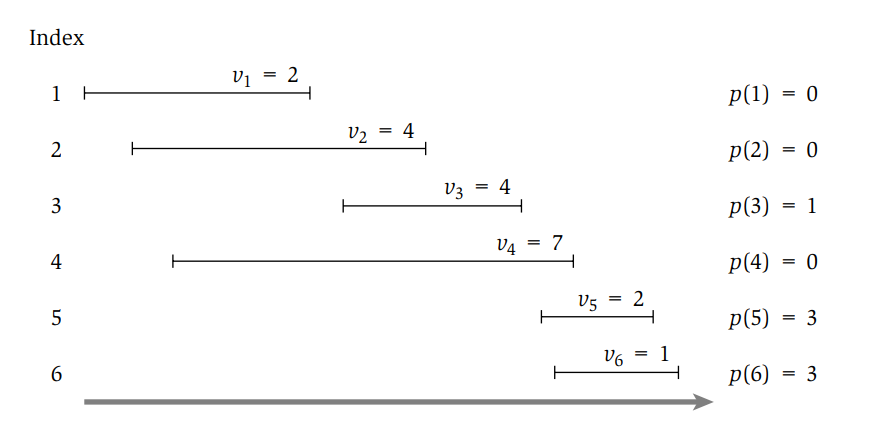
\includegraphics[width=12cm, keepaspectratio]{capitoli/imgs/weighted_problem.png}
    \caption{Istanza di un problema.}
\end{figure}

\section{Goal \normalfont{\emoji{soccer-ball}}}

L'obiettivo del nostro problema attuale è quello di trovare un sottoinsieme $S
    \subseteq \{1, \ldots, n\}$ di intervalli mutualmente compatibili che vanno a
massimizzare la somma dei pesi degli intervalli selezionati $\sum_{i \in S}
    v_i$.

\section{Funzionamento}

Come prima cosa definiamo il metodo per calcolare $OPT(j)$. Il problema è
una \textit{scelta binaria} che va a decidere se l'intervallo di indice $j$
verrà incluso nella soluzione oppure no basandosi sul valore ritornato dalla
seguente formula:

\begin{equation}
    \label{eqn:weight-opt}
    OPT(j) = max(v_j + OPT(p(j)), \ \ OPT(j-1))
\end{equation}
\ \\
Questo può essere anche visto come una disequazione:

\begin{equation}
    \label{eqn:weight-opt-dis}
    v_j + OPT(p(j)) \geq OPT(j-1)
\end{equation}
\ \\
che se vera, includerà $j$ nella soluzione ottimale.

\pagebreak

Scrivendo tutto sotto forma di algoritmo ricorsivo avremmo che:

\begin{lstlisting}[language=Javascript]
    function Compute-Opt(j){
        if (j == 0)
            return 0
        else
            return max(vj+Compute-Opt(p(j)), Compute-Opt(j − 1))
    }
\end{lstlisting}

Costruendo l'albero della ricorsione dell'algoritmo si nota che la complessità
temporale è esponenziale \emoji{astonished} !

\begin{figure}[H]
    \centering
    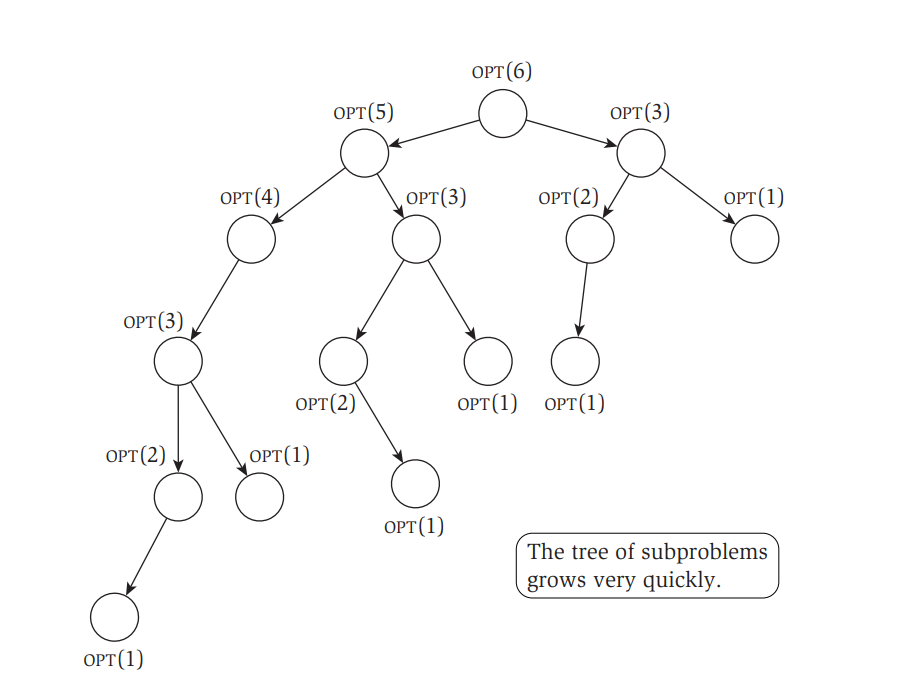
\includegraphics[width=12cm, keepaspectratio]{capitoli/imgs/opt_albero.png}
    \caption{Sviluppo dell'albero di ricorsione per la risoluzione di un problema.}
\end{figure}

\pagebreak

Una soluzione è quella di utilizzare la tecnica della \textbf{Memoization} che evita
di ricalcolare $OPT$ per gli indici già calcolati precedentemente, rendendo così
il costo temporale uguale ad $O(n)$ \emoji{man-in-motorized-wheelchair}.

\begin{lstlisting}[language=Javascript]
function M-Compute-Opt(j){
    if (j == 0)
        return 0
    else if (M[j] is not empty)
        return M[j]
    else
        let M[j] = max(vj+M-Compute-Opt(p(j)), M-Compute-Opt(j-1))
        return M[j]
}
\end{lstlisting}

Oltre al valore della soluzione ottimale probabilmente vorremmo sapere anche
quali sono gli intervalli che la compongono, e intuitivamente verrebbe da creare
un array aggiuntivo in cui verranno aggiunti gli indici degli intervalli
ottenuti con \verb|M-Compute-Opt|. Tuttavia questo aggiungerebbe una complessità
temporale di $O(n)$ peggiorando notevolmente le prestazioni. Un'alternativa è
quella di recuperare le soluzioni dai valori salvati nell'array \verb|M| dopo che la
soluzione ottimale è stata calcolata. Per farlo possiamo sfruttare la formula
vista in precedenza $v_j + OPT(p(j)) \geq OPT(j-1)$, che ci permette di
rintracciare gli intervalli della soluzione ottima.

\begin{lstlisting}[language=Javascript]
    function Find-Solution(j) {
        if (j == 0)
            Output nothing
        else if (vj + M[p(j)] >= M[j-1])
            Output j together with the result 
            of Find-Solution(p(j))
        else
            Output the result of Find-Solution(j-1)
    }
\end{lstlisting}
% \chapter{Least Squares Problem: Multi-way Choice \normalfont{\emoji{motorway}}}

Nel capitolo precedente l'algoritmo richiedeva una ricorsione basata su scelte
binarie, in questo capitolo invece introdurremo un algoritmo che richiede ad
ogni step un numero di scelte polinomiali (\textit{multi-way choice}). Vedremo
come la programmazione dinamica si presta molto bene a risolvere questi
problemi.

\section{Linear Least Square}

\subsection{Il Problema}

La formulazione del problema è la seguente:

\paragraph*{} dato un insieme $P$ composto di $n$ punti sul piano denotati con\\
$(x_1, y_1), (x_2, y_2), \ldots, (x_n, y_n)$; e supponiamo che $x_1 < x_2 <
    \ldots < x_n$ (sono strettamente crescenti). Data una linea $L$ definita
dall'equazione $y = ax + b$, definiamo l'\textit{errore} di $L$ in funzione
di $P$ come la somma delle distanze al quadrato della linea rispetto ai
punti in $P$. Formalmente:
\[
    Error(L, P) = \sum_{i=1}^{n} (y_i - ax_i - b)^2
\]

\begin{figure}[H]
    \centering
    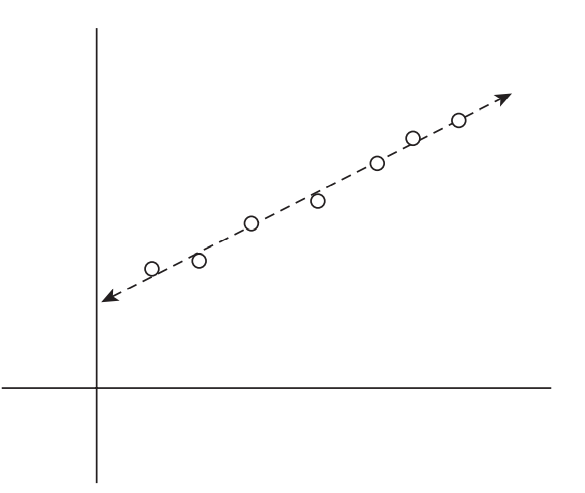
\includegraphics[width=6cm, keepaspectratio]{capitoli/imgs/linear_least.png}
    \caption{Esempio di una tipica istanza e soluzione del problema
        \textit{Linear Least}}
\end{figure}

\subsection{\goal}

È intuibile che il goal dell'algoritmo è quello di cercare la linea con errore
minimo, che può essere facilmente trovata utilizzando l'analisi matematica.
La linea di errore minimo è $y = ax + b$ dove:

\[
    a = \frac{n \sum_{i} x_i y_i - (\sum_{i} x_i) (\sum_{i} y_i)}{n \sum_{i} x_i^2 - (\sum_{i} x_i)^2} \ \ \  \ \ b = \frac{\sum_{i} y_i - a \sum_{i} x_i}{n}
\]

\section{Segmented Least Square}

Le formule appena citate sono utilizzabili solo se i punti di $P$ hanno un
andamento che è abbastanza lineare ma falliscono in altre circostanze.

\begin{figure}[H]
    \centering
    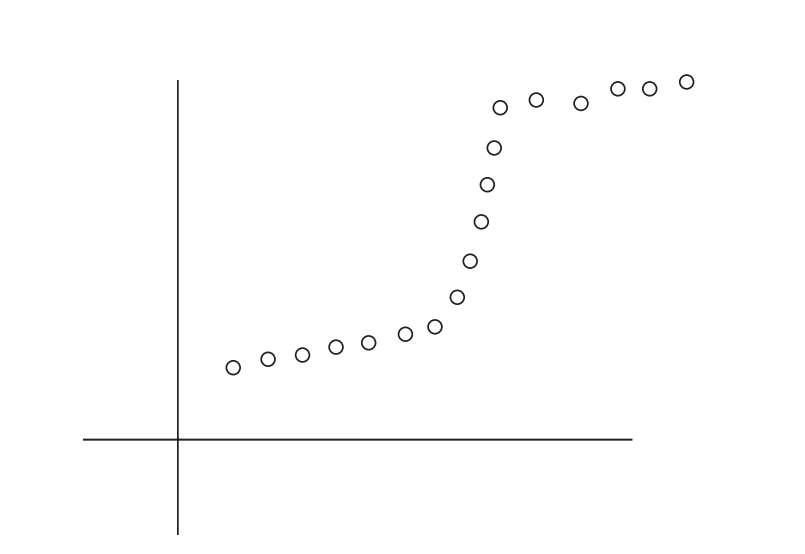
\includegraphics[width=8cm, keepaspectratio]{capitoli/imgs/segmente_linear_least.png}
    \caption{Esempio di funzione non risolvibile con Linear Least Square}
\end{figure}

Come è evidente (\textit{lapalissiano \normalfont{\emoji{gem}}}) dalla figura
non è possibile trovare una linea che approssimi in maniera soddisfacente i
punti, dunque per risolvere il problema possiamo pensare di rilassare la
condizione che sia solo una la linea. Questo però implica dover riformulare il
goal che altrimenti risulterebbe banale (si fanno $n$ linee che passano per ogni
punto).

\subsection{Costi}

La parte che computa gli errori ha costo in tempo $O(n^3)$ (si può portare a
$O(n^2)$).
La parte che trova il valore ottimo ha costo $O(n^2)$.\\

In spazio l'algoritmo ha costo $O(n^2)$ ma può essere ridotto a $O(n)$

\subsection{\goal}

Formalmente, il problema è espresso come segue:

\paragraph*{} come prima abbiamo un set di punti $P = \{(x_1, y_1), (x_2, y_2),
    \ldots, (x_n, y_n)\}$ strettamente crescenti. Denoteremo l'insieme dei punti
$(x_i, y_i)$ con $p_i$. Vogliamo partizionare $P$ in un qualche numero di
segmenti, ogni numero di segmenti è un sottoinsieme di $P$ che rappresenta un
\textit{set} contiguo delle coordinate $x$ con la forma $\{p_i, p_{i+1}, \ldots,
    p_{j-1}, p_j\}$ per degli indici $i \leq j$. Dopodiché, per ogni segmento $S$
calcoliamo la linea che minimizza l'errore rispetto ai punti in $S$ secondo
quanto espresso dalle formule enunciate prima.\\

Definiamo infine una penalità per una data partizione come la somma dei seguenti
termini:

\begin{itemize}
    \item Numero di segmenti in cui viene partizionato $P$ moltiplicato per un
          valore $C > 0$ (più è grande e più penalizza tante partizioni)
    \item Per ogni segmento l'errore della linea ottima attraverso quel
          segmento.
\end{itemize}


Il goal del Segmented Least Square Problem è quindi quello di trovare la
partizione di \textbf{penalità minima}.

\subsection{Funzionamento}

Per come è fatta la programmazione dinamica noi vogliamo suddividere il problema
in sotto-problemi e per farlo partiamo dall'osservazione che l'ultimo punto
appartiene ad una partizione ottima che parte da un valore $p_i$ fino a $p_n$ e
che possiamo togliere questi punti dal totale per ottenete un sotto-problema più
piccolo. Supponiamo che la soluzione ottima sia denotata da \verb|OPT(j)|, per i
punti che vanno da $p_1$ a $p_j$, allora avremo che la soluzione ottima al
problema dato l'ultimo segmento che va da $p_i$ a $p_n$, sarà dalla seguente
formula:

\[
    OPT(n) = e_{i,n} + C + OPT(i - 1)
\]

Questa formula è data dalla soluzione ottima dell'ultima partizione ($e_{i,n} + C$)
a cui viene aggiunta la soluzione ottima di tutte le partizioni precedenti
($OPT(i -1)$). Per i sotto-problemi possiamo scrivere la soluzione al problema
in forma ricorsiva utilizzando la formula appena espressa che prenderà la forma:

\[
    OPT(j) = \min_{1 \leq i \leq j}(e_{i,j} + C + OPT(i - 1))
\]

Possiamo ora dare una versione di questo algoritmo in pseudocodice:

\begin{lstlisting}[language=Javascript]
    function Segmented-Least-Squares(n) {
        M[0 ... n]
        M[0] = 0

        // compute the errors
        for (j in 1 ... n) {
            for (i in 1 ... j) {
                compute eij for the segment pi, ..., pj
            }
        }

        // find optimal value
        for (j in 1 ... n) {
            M[j] = min_i(eij + C + M[i - 1]) // OPT(J)
        }

        return M[n]
    }
\end{lstlisting}

Dopo aver trovato la soluzione ottima, possiamo sfruttare la memoization per
ricavarci i segmenti in tempi brevi.

\begin{lstlisting}[language=Javascript]
    function Find-Segments(j) {
        if (j == 0) print('')

        else {
            Find an i that minimizes ei,j + C + M[i − 1]
            Output the segment {pi,..., pj} and the result of Find-Segments(i − 1)
        }
    }
\end{lstlisting}

L'algoritmo ha costo $O(n^3)$ in tempo e $O(n^2)$ in spazio.
Questo tempo può essere ridotto applicando la memoization alle formule per il calcolo
dell'errore viste in precedenza portandolo a $O(n^2)$ per il tempo e $O(n)$ per lo spazio.
% \chapter{Subset Sum \& Knapsack Problem \normalfont{\emoji{money-bag}}}

\section{Il Problema}

Il problema delle Subset Sum è formalmente definito come segue:\\

\- abbiamo $n$ oggetti $\{1, \ldots, n\}$, a ognuno viene assegnato un
peso non negativo $w_i$ (per $i = 1, \ldots, n$) e ci viene dato anche un
limite $W$. L'obbiettivo è quello di selezionare un sottoinsieme $S$ degli
oggetti tale che $\sum_{i \in S}w_i \leq W$ e che questa sommatoria abbia valore
più grande possibile.\\

Questo problema è un caso specifico di un problema più generale conosciuto come
il Knapsack Problem, l'unica differenza sta nel valore da massimizzare che per il
Knapsack è un valore $v_i$ e non più il peso.

Si potrebbe pensare di risolvere questi problemi con un algoritmo greedy ma
purtroppo non ne esiste uno in grado di trovare efficientemente la soluzione ottima.
Potremmo pensare di ordinare gli oggetti in base al peso in ordine crescente o
decrescente e prenderli, tuttavia questo approccio fallisce per determinati casi
(come per l'insieme $\{W/2+1, W/2, W/2\}$ ordinato in senso decrescente) e l'unica
opzione sarà quella di provare con la programmazione dinamica \emoji{person-in-manual-wheelchair}.
\newpage

\section{\goal}

Possiamo riassumere il goal di questi problemi come segue:\\

\- Abbiamo $n$ oggetti $\{1, \ldots, n\}$, a ognuno viene assegnato un
peso non negativo $w_i$ (per $i = 1, \ldots, n$) e ci viene dato anche un
limite $W$. L'obbiettivo è quello di selezionare un sottoinsieme $S$ degli oggetti
tale che $\sum_{i \in S}w_i \leq W$ e che questa sommatoria abbia valore più
grande possibile.

\section{Costi}

\begin{center}
    \begin{tabular}{|c|c|}
        \centering
        \textbf{Funzione}    & \textbf{Costo (tempo)} \\
        \verb|Subset-Sum|    & $O(nW)$                \\
        \verb|Find-Solution| & $O(n)$                 \\
    \end{tabular}
\end{center}

\section{Funzionamento}

Come per tutti gli algoritmi dinamici dobbiamo cercare dei sotto-problemi e
possiamo utilizzare la stessa intuizione avuto per il problema dello scheduling
(scelta binaria). Facendo tutti i calcoli di dovere otteniamo la seguente
ricorsione:

\begin{center}
    se $w < w_i$ allora $OPT(i, w) = OPT(i-1,w)$ altrimenti\\
    $OPT(i, w) = max(OPT(i-1, w), w_i + OPT(i-1, w-w_i))$
\end{center}

Nella prima parte analizziamo il caso in cui l'elemento che vogliamo aggiungere va
a superare il peso massimo residuo $w$, dunque viene scartato. Nella seconda parte
andiamo ad analizzare se l'aggiunta o meno del nuovo oggetto va a migliorare
la soluzione di $OPT$ che è definita come:\\

\[
    OPT(i, w) = \max_{S} \sum_{j \in S} w_j
\]
\newpage

Possiamo formalizzare il tutto con il seguente pseudo-codice:

\begin{lstlisting}[language=JavaScript]
    function Subset-Sum(n, W) {
        let M[0 . . . n,0... W]

        //initialize the memoization vector
        for(w in 0 ... W) {
            M[0, W] = 0
        }

        //solve subproblems
        for(i in 1 ... n) {
            for(w in 0 ... W) {
                Use the recurrence to compute M[i, w]
            }
        }

        return M[n, W]
    }
\end{lstlisting}

La particolarità di questo algoritmo è che avremmo 2 insiemi di sotto-problemi
diversi che devono essere risolti per ottenere la soluzione ottima. Questo fatto
si riflette in come viene popolato l'array di memoization dei valori di $OPT$
che verranno salvati in un array bidimensionale.

\begin{figure}[H]
    \centering
    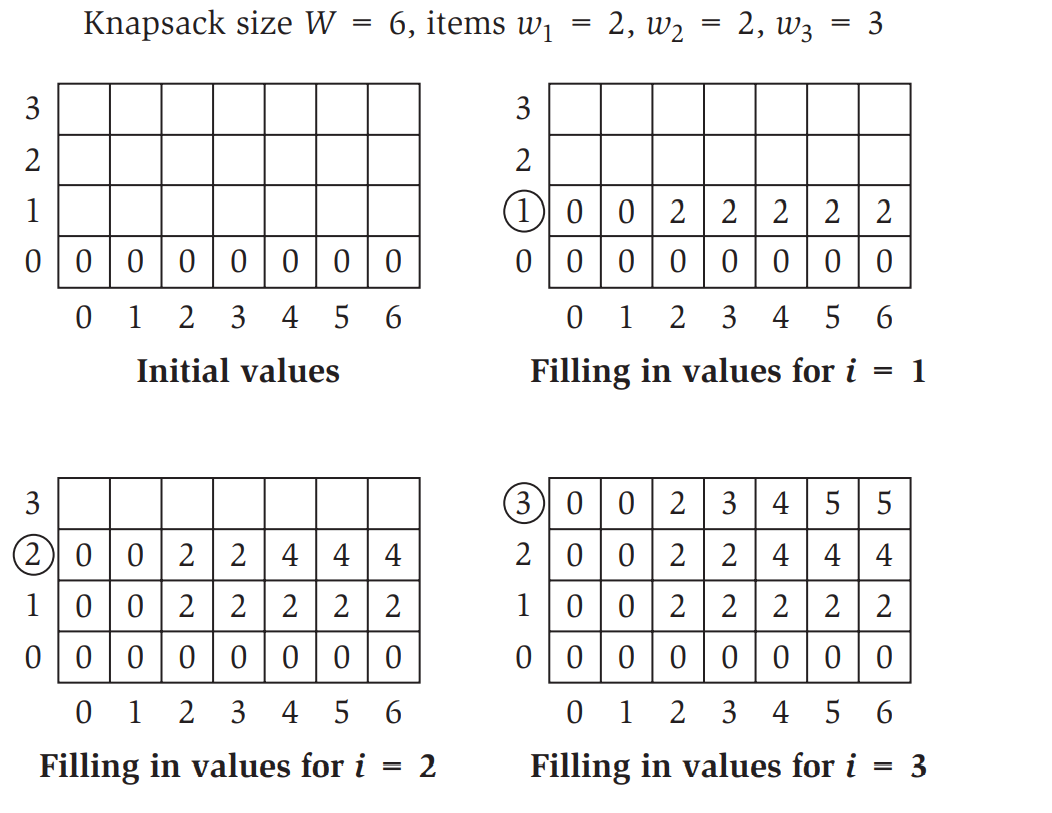
\includegraphics[width=10cm, keepaspectratio]{capitoli/imgs/knapsac_table.png}
    \caption{Esempio di come viene popolato l'array $M$ per il problema del Knapsack.}
\end{figure}

\textit{Il costo in tempo di questa implementazione è di $O(nW)$.}\\

A causa di questo costo, l'algoritmo fa parte della famiglia degli
algoritmi \textit{pseudo polinomiali}, ovvero algoritmi il cui costi dipende da
una variabile di input che se piccola, lo mantiene basso e se grande lo fa
esplodere.\\

\textit{Per recuperare gli oggetti dall'array di Memoization la complessità in tempo è di
    $O(n)$.}\\

Questa implementazione funziona anche per il problema più generale del Knapsack,
ci basterà solo cambiare la parte di ricorsione scrivendola come segue:

\begin{center}
    se $w < w_i$ allora $OPT(i, w) = OPT(i-1,w)$ altrimenti
    $OPT(i, w) = max(OPT(i-1, w), v_i + OPT(i-1, w-w_i))$
\end{center}

La complessità temporale è sempre $O(nW)$.
% \section{RNA Secondary Structure \normalfont{\emoji{dna}}}

La ricerca della struttura secondaria dell'RNA è un problema a 2 variabili
risolvibile tramite il paradigma della programmazione dinamica. Come sappiamo il
DNA è composto da due filamenti, mentre l'RNA è composto da un filamento
singolo. Questo comporta che spesso le basi di un singolo filamento di RNA si
accoppino tra di loro. L'insieme della basi può essere visto come l'alfabeto
$\{A, C, U, G\}$ e l'RNA è una sequenza di simboli presi da questo alfabeto. Il
processo di accoppiamento delle basi è dettato dalla regola di \textit{Watson-Crick} e
segue il seguente schema:

\[
    A - U \ \ \ \textrm{ e } \ \ \ C - G \ \ \ \textrm{ (l'ordine non conta)}
\]

\begin{figure}[H]
    \centering
    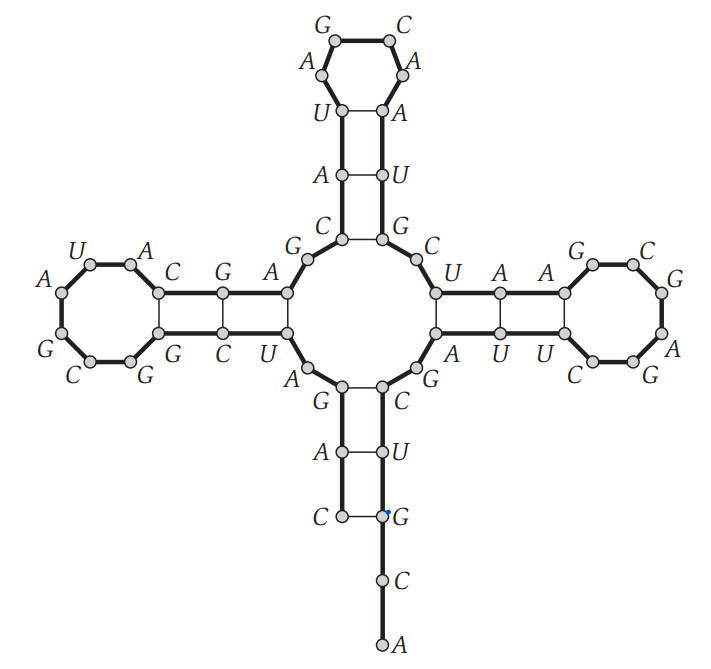
\includegraphics[width=8cm, keepaspectratio]{capitoli/dynamic_programming/imgs/rna_esempio1.png}
    \caption{Esempio di una struttura secondari di RNA} %%TODO: ricontrollare !!
\end{figure}

\subsection{Il Problema}

In questo problema si vuole trovare la struttura secondaria dell'RNA che abbia
energia libera maggiore (il maggior numero di coppie di basi possibili). Per
farlo dobbiamo tenere in considerazione alcune condizioni che devono essere
soddisfatte per permettere di approssimare al meglio il modello biologico
dell'RNA.\\

Formalmente la struttura secondaria di $B$ è un insieme di coppie $S =
    \{(i,j)\}$ dove $i,j \in \{1,2,\ldots,n\}$, che soddisfa le seguenti
condizioni:

\begin{enumerate}
    \item \textbf{No Sharp Turns}: la fine di ogni coppia è separata da almeno 4
          basi, quindi se $(i,j) \in S$ allora $i < j - 4$
    \item Gli elementi di una qualsiasi coppia $S$ consistono di $\{A, U\}$ o
          $\{C, G\}$ (in qualsiasi ordine).
    \item $S$ è un \textit{matching}: nessuna base compare in più di una coppia.
    \item \textbf{Non Crossing Condition}: se $(i, j)$ e $(k,l)$ sono due coppie
          in $S$ allora \textbf{non} può avvenire che $i < k < j < l$.
\end{enumerate}

\begin{figure}[H]
    \centering
    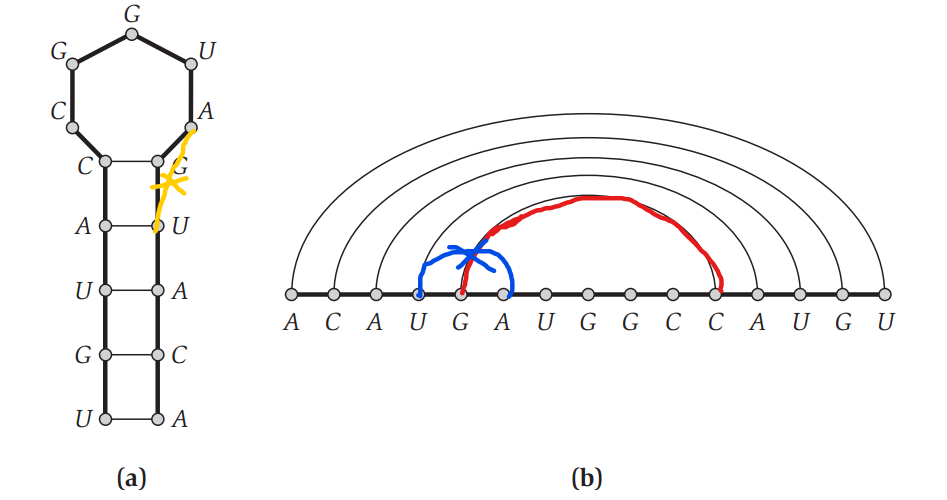
\includegraphics[width=10cm, keepaspectratio]{capitoli/dynamic_programming/imgs/rna_esempio2.png}
    \caption{La figura \textit{(a)} rappresenta un esempio di \textit{Sharp
            Turn}, mentre la figura \textit{(b)} mostra una
        \textit{Crossing Condition} dove il filo blu non dovrebbe esistere.}
\end{figure}

\subsection{\goal}

Il goal di questo problema è di massimizzare la quantità di coppie che si possono
formare all'interno della struttura secondaria di una data sequenza di RNA.

\subsection{Costi}

L'algoritmo complessivo ha costo $O(n^3)$.

\subsection{Funzionamento}

\paragraph{First Attempt.}
Come primo tentativo potremmo basarci sul seguente sotto-problema: affermiamo che
$OPT(j)$ è il massimo numero di coppie di basi sulla struttura secondaria $b_1
    b_2 \ldots b_j$, per la Non Sharp Turn Condition sappiamo che $OPT(j) = 0$ per
$j \leq 5$ e sappiamo anche che $OPT(n)$ è la soluzione che vogliamo trovare. Il
problema ora sta nell'esprimere $OPT(j)$ ricorsivamente. Possiamo parzialmente
farlo sfruttando le seguenti scelte:

\begin{itemize}
    \item $j$ non appartiene ad una coppia
    \item $j$ si accoppia con $t$ per qualche $t \leq
              j - 4$
\end{itemize}

Per il primo caso basta cercare la soluzione per $OPT(j - 1)$, nel secondo caso
invece se teniamo conto della Non Crossing Condition, possiamo isolare due nuovi
sotto-problemi: uno sulle basi $b_1 b_2 \ldots b_{t-1}$ e l'altro sulle basi
$b_{t+1} \ldots b_{j-1}$. Il primo si risolve con $OPT(t-1)$ ma il secondo, dato
che non inizia con indice $1$, non è nella lista dei nostri sotto-problemi. A
causa di ciò risulta necessario aggiungere una variabile.

\begin{figure}[H]
    \centering
    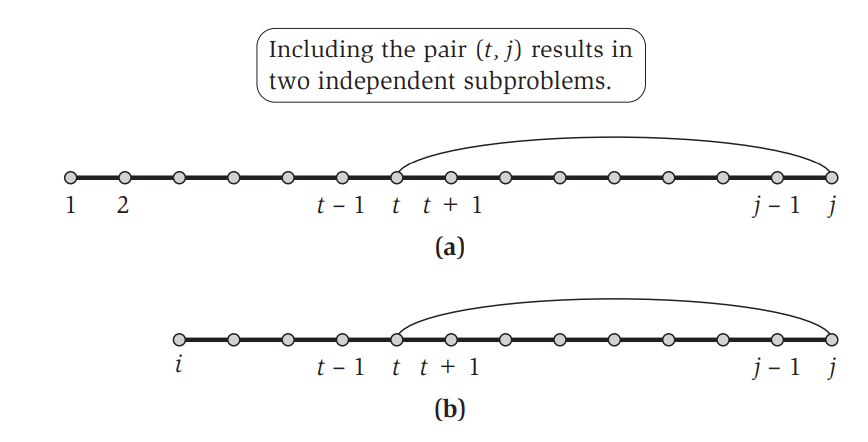
\includegraphics[width=10cm, keepaspectratio]{capitoli/dynamic_programming/imgs/rna_funzionamento.png}
    \caption{Esempio di
        utilizzo di una sola variabile \textit{(a)} o con due \textit{(b)}.}
\end{figure}

\paragraph{Dynamic Programming over Intervals}
Basandoci sui ragionamenti precedenti, possiamo scrivere una ricorsione di
successo: sia $OPT(i,j)$ il numero massimo di coppie di basi nella struttura
secondaria $b_i b_{i+1} \ldots b_j$, grazie alla non sharp turn Condition
possiamo inizializzare gli elementi con $i \geq j -4$ a $0$. Ora avremmo sempre
le stesse condizioni elencate sopra:

\begin{itemize}
    \item $j$ non appartiene ad una coppia
    \item $j$ si accoppia con $t$ per qualche $t \leq j - 4$
\end{itemize}

Nel primo caso avremmo che $OPT(i,j) = OPT(i, j-1)$, nel secondo caso possiamo
ricorrere su due sotto-problemi $OPT(i, t-1)$ e $OPT(t+1, j-1)$ affinché venga
rispettata la non crossing condition. Possiamo esprimere formalmente la
ricorsione come segue:

\begin{center}
    \[
        OPT(i, j) = \max(OPT(i, j-1), \max_t(1+OPT(i, t-1)+OPT(t+1, j-1))),
    \]
    dove il massimo è calcolato su $t$ tale che $b_t$ e $b_j$ siano una coppia di
    basi consentita
\end{center}

\begin{figure}[H]
    \centering
    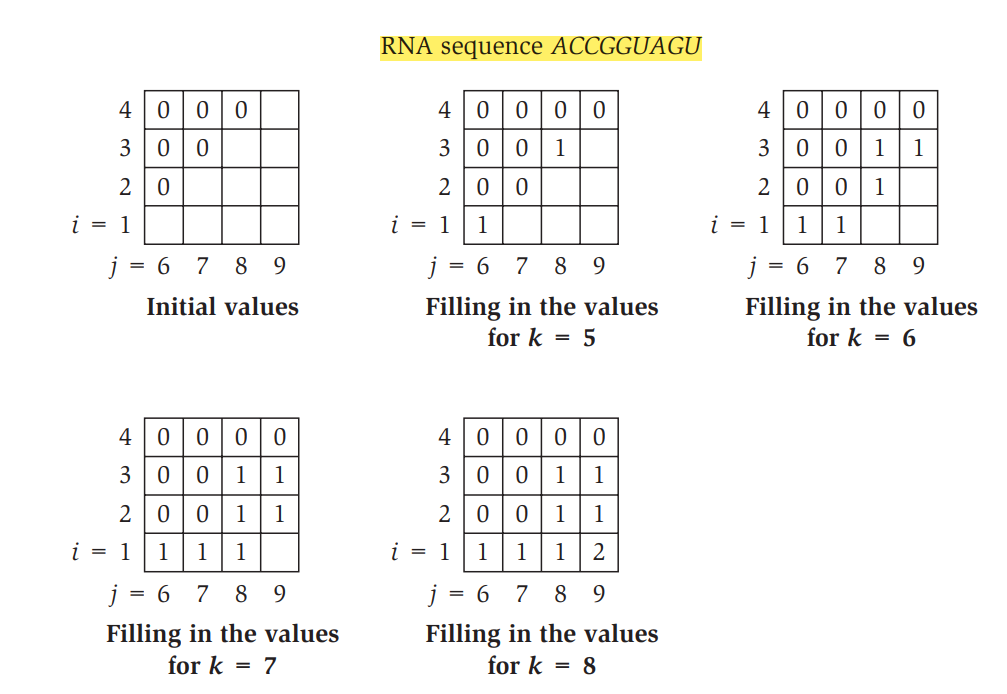
\includegraphics[width=\textwidth, keepaspectratio]{capitoli/dynamic_programming/imgs/rna_calcolo.png}
    \caption{Iterazioni dell'algoritmo su un campione del problema in questione $ACCGGUAGU$}
\end{figure}
\newpage

Possiamo infine formalizzare il tutto con il seguente pseudo-codice:

\begin{lstlisting}[language=JavaScript]
 Initialize OPT(i, j) = 0 whenever i ≥ j - 4

 for (k in 5 ... n - 1) {
     for (i in 1 ... n - k) {
         j = i + k
         Compute OPT(i, j) using the previous recurrence
     }
 }

 return OPT(1, n)
\end{lstlisting}

Ci sono $O(n^2)$ sotto-problemi da risolvere e ognuno richiede tempo $O(n)$,
quindi il running time complessivo è di $O(n^3)$.

% \section{Sequence Alignment}

Il problema del Sequence Alignment consiste nel riuscire a comparare delle
stringhe, come per esempio quando si effettua un typo in un motore di ricerca e
quello ci fornisce l'alternativa corretta. Una prima idea potrebbe essere quella
di \textbf{allineare} le due parole lettera per lettera, riempendo gli eventuali
spazi bianchi, e vedendo di quanto le due differiscono. Tuttavia ci sono varie
possibilità con cui due parole di lunghezza diversa possono essere confrontate,
quindi è necessario fornire una definizione di \textbf{similarità}.

\subsection{Il Problema}

Come prima definizione di similarità possiamo dire che minore sarà il numero di
caratteri che non corrispondono, maggiore sarà la similarità tra le parole.
Questa problematica è anche un tema centrale della biologia molecolare, e
proprio grazie ad un biologo abbiamo una definizione rigorosa e soddisfacente di
similarità. Prima di dare una definizione similarità dovremo però darne una di
\textbf{allineamento}: Supponiamo di avere due stringhe $X$ e $Y$, che consistono rispettivamente
della sequenza di simboli $x_1 x_2 \ldots x_m$ e $y_1 y_2 \ldots y_n$, e
consideriamo gli insiemi $\{1,2,\ldots ,m\}$ e $\{1,2,\ldots ,n\}$ che
rappresentano le varie posizioni nelle stringhe $X$ e $Y$, ora si considera un
\textbf{Matching} di queste due parole (un matching è stato definito nella parte
precedente e si tratta di un insieme di coppie ordinate con la proprietà che
ogni oggetto si trova al più in una sola coppia).  Diciamo ora che un matching
$M$ di questi due insiemi è un allineamento se gli elementi di varie coppie non
si incrociano: se $(i,j),(i^{\prime},j^{\prime}) \in M$  e $i < i^{\prime}$,
allora $j < j^{\prime}$.\\

Ora la nostra definizione di similarità si baserà sul trovare il miglior
allineamento, seguendo i seguenti criteri:

\begin{itemize}
    \item C'è un parametro $\delta>0$ che
          definisce la \textbf{gap penalty}, ovvero ogni volta che un simbolo di una parola
          non corrisponde ad un simbolo dell'altra.
    \item Per ogni coppia di lettere $p,q$ del
          nostro alfabeto, se c'è un accoppiamento errato si paga il corrispondente
          \textbf{mismatch cost} $a_(p,q)$.
    \item Il costo di $M$ è la somma del suo gap e mismatch
          cost, e l'obiettivo sarà quello di minimizzarlo.
\end{itemize}

\subsection{Creazione dell'algoritmo}

Ora affronteremo il problema di calcolarci questo costo minimo, e l'allineamento
ottimale che lo fornisce date le coppie $X$ e $Y$. Come al solito proveremo con
un approccio di programmazione dinamica, e per realizzare l'algoritmo
individuiamo come per altri algoritmi già visti una scelta binaria. Dato
l'allineamento ottimale $M$ allora:

\begin{itemize}
    \item $(m,n) \in M$ (quindi gli ultimi due
          simboli delle 2 stringhe sono in un matching)
    \item $(m,n) \notin M$ (gli ultimi
          simboli delle due stringhe non sono in un matching)
\end{itemize}

Tuttavia questa semplice distinzione non è sufficiente, quindi supponiamo di
aggiungere anche il seguente fatto elementare:\\

\- Sia $M$ un qualsiasi allineamento di $X$ e $Y$. se $(m,n) \notin M$, allora o
l' $m-esima$ posizione di $X$ o l' $n-esima$ posizione di $Y$ non è in un
matching di $M$.\\

Dire questo equivale a riscrivere le due condizioni sopra come tre, dunque in un
allineamento ottimo $M$ almeno una deve essere vera:

\begin{itemize}
    \item $(m,n) \in M$
    \item l'$m-esima$ posizione di $X$ non è nel matching
    \item l' $n-esima$ posizione di $Y$ non è nel matching
\end{itemize}

Ora definiamo la funzione di costo minimo $OPT(i,j)$ come costo dell'alignmet
tra $x_1 x_2 \ldots x_i$ e $y_1 y_2 \ldots y_j$. In base alle condizioni
espresse in precedenza la funzione $OPT(m,n)$ assumerà il costo relativo più
$OPT(m-1,n-1)$, in particolare (i tre casi citati sopra):

\begin{itemize}
    \item condizione 1, si
          paga un matching cost per le lettere $m,n$
    \item condizione 2 e 3, si paga un gap
          cost $\delta$ per $m$(condizione 2) o $n$(condizione 3)
\end{itemize}

Utilizzando dunque gli stessi argomenti per per i sotto problemi per
l'allineamento di costo minimo tra $X$ e $Y$ otteniamo la definizione generale
di $OPT(i,j)$:\\

L'allineamento di costo minimo soddisfa la seguente ricorsione per $i \geq 1$
e $j \geq 1$:
\[
    OPT(i,j) = min[a_{(x_i y_j)} + OPT(i-1, j-1),
            \delta + OPT(i-1, j), \delta + OPT(i, j-1)]
\]

Dunque così abbiamo ottenuto la nostra funzione di ricorsione e possiamo
procedere alla scrittura dello pseudo codice.

\begin{lstlisting}[language=JavaScript]
    function alignment(X,Y) { var A = Matrix(m, n)

        Initialize A[i, 0]= iδ for each i 
        Initialize A[0, j]= jδ for each j

        for (j in 1...n) { 
            for (i in 1...m) { 
                Use the recurrence (6.16) to compute A[i, j] 
            }
        }

        return A[m, n]
    }
\end{lstlisting}

Il running time è di $O(mn)$

\subsection{Sequence Alignment in Spazio Lineare}

Come abbiamo appena visto l'algoritmo ha sia costo spaziale che temporale uguale
a $O(mn)$ e se come input consideriamo le parole della lingua inglese non
risulta essere un grande problema, ma se consideriamo genomi con 10 miliardi di
caratteri potrebbe risultare difficile poter lavorare con array di 10 GB \emoji{astonished}.
Questo problema può essere risolto utilizzando un approccio \textit{divide et impera}
che va a rendere lineare il costo dello spazio ( $O(n + m)$ ).

\subsubsection{Funzionamento}

Come prima cosa definiamo un algoritmo Space Efficient Alignment che ci permette
di trovare la soluzione ottima utilizzando il minor spazio possibile. Per farlo
notiamo che la funzione $OPT$ dipende solamente da una colonna precedente di
quella che si sta analizzando, dunque basterà caricarsi in memoria una matrice
$mx2$ riducendo così il costo spaziale ad $m$. Tuttavia utilizzando questo
metodo non e possibile ricurvare l'alignment effettivo perché non ci bastano le
informazioni.\\

Lo pseudo-codice dell'algoritmo appena definito è il seguente:

\begin{lstlisting}[language=JavaScript]
    function Space-Efficient-Alignment(X,Y) {
        var B = Matrix(m, 2)

        // (just as in column 0 of A)
        Initialize B[i, 0]= iδ for each i 

        for (j in 1...n) {
            B[0, 1]= jδ (since this corresponds to entry A[0, j])

            for (i in 1...m) {
                B[i, 1]= min[
                    αxiyj + B[i − 1, 0],
                    δ + B[i − 1, 1], 
                    δ + B[i, 0]
                ]
            }

            Move column 1 of B to column 0 to make room 
            for next iteration:
            Update B[i, 0] = B[i, 1] for each i
        }
    }
\end{lstlisting}

Possiamo quindi utilizzare un approccio \textit{divide et impera} che incorpora 2
tecniche diverse di programmazione dinamica per sfruttare questo approccio
appena definito e riuscire a trovare anche l'alignment in spazio lineare.
Definiamo quindi due funzioni:

\begin{itemize}
    \item $f(i, j)$ : è la funzione definita per l'algoritmo di Sequence
          Alignment di base (analoga a $OPT(i,j)$ )
    \item $g(i, j)$ : è l'analogo al contrario di $f$ ed è definito dalla
          seguente funzione ricorsiva: per $i < m$ e $j < n$ : $g(i,j) =
              min[a_{x+1y+1} + g(i+1, j+1), \delta + g(i, j+1), \delta + g(i+1, j)]$
\end{itemize}

Possiamo notare che la ricorsione $f$ procede a ritroso partendo dal fondo
mentre la ricorsione $g$ procede in avanti partendo dall'inizio. Possiamo
sfruttare questo fatto per provare ad utilizzare lo Space Efficiente Sequence
Alignment Algorithm combinato ad un approccio \textit{divide et impera} e un array di
supporto $P$ per riuscire a calcolare il Sequence Alignment in spazio lineare,
aumentando solo di una costatane la complessità temporale.\\

Possiamo riassumere il tutto con il seguente pseudo-codice:

\begin{lstlisting}[language=JavaScript]
    function Divide-and-Conquer-Alignment(X,Y) {
        var m = length(X)
        var n = length(Y)

        if (m <= 2 or n <= 2) {
            Compute optimal alignment using Alignment(X,Y)
        }

        Space-Efficient-Alignment(X, Y[1 : n/2])
        Backward-Space-Efficient-Alignment(X, Y[n/2 + 1 : n])

        Let q be the index minimizing f(q, n/2) + g(q, n/2)
        Add (q, n/2) to global list P

        Divide-and-Conquer-Alignment(X[1 : q],Y[1 : n/2])
        Divide-and-Conquer-Alignment(X[q + 1 : n],Y[n/2 + 1:n])

        return P
    }
\end{lstlisting}

\begin{figure}[H]
    \centering
    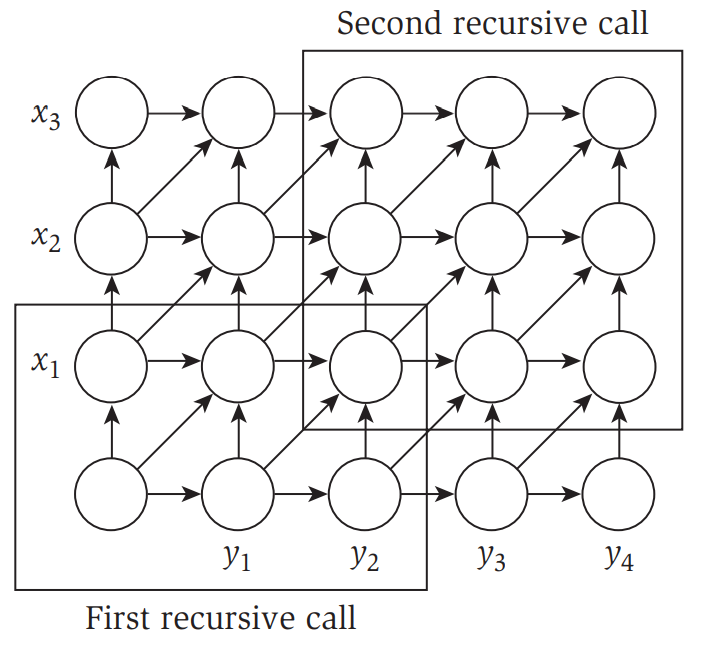
\includegraphics[width=8cm, keepaspectratio]{capitoli/dynamic_programming/imgs/seq_align_recurrence.png}
    \caption{La figura mostra il funzionamento dell'algoritmo appena descritto.}
\end{figure}

\documentclass[a4paper,12 pt]{report}
\usepackage[T1]{fontenc}
\usepackage[utf8]{inputenc}
% \usepackage{amsmath}
\usepackage{lmodern}
\usepackage{listings}
\usepackage{graphicx}
\usepackage{float}
\usepackage{subcaption}
\usepackage{hyperref}
\usepackage{wrapfig}
\usepackage{fancyhdr}
% \usepackage{tcolorbox}

% forza le footnote a stare il più in basso possibile
\usepackage[bottom]{footmisc}
\usepackage{enumitem}

%% STILE LISTINGS

\usepackage{xcolor}

\definecolor{codegreen}{rgb}{0,0.6,0}
\definecolor{codegray}{rgb}{0.5,0.5,0.5}
\definecolor{codepurple}{rgb}{0.58,0,0.82}
\definecolor{backcolour}{rgb}{0.95,0.95,0.92}

\lstdefinestyle{mystyle}{
    backgroundcolor=\color{backcolour},   
    commentstyle=\color{codegreen},
    keywordstyle=\color{magenta},
    numberstyle=\tiny\color{codegray},
    stringstyle=\color{codepurple},
    basicstyle=\ttfamily\footnotesize,
    breakatwhitespace=false,         
    breaklines=true,                 
    captionpos=b,                    
    keepspaces=true,                 
    numbers=left,                    
    numbersep=5pt,                  
    showspaces=false,                
    showstringspaces=false,
    showtabs=false,                  
    tabsize=2
}

\lstset{style=mystyle}

%% SOLIDITY Settings

% Copyright 2017 Sergei Tikhomirov, MIT License
% https://github.com/s-tikhomirov/solidity-latex-highlighting/

%\usepackage{listings, xcolor}

\definecolor{verylightgray}{rgb}{.97,.97,.97}

\lstdefinelanguage{Solidity}{
	keywords=[1]{anonymous, assembly, assert, balance, break, call, callcode, case, catch, class, constant, continue, constructor, contract, debugger, default, delegatecall, delete, do, else, emit, event, experimental, export, external, false, finally, for, function, gas, if, implements, import, in, indexed, instanceof, interface, internal, is, length, library, log0, log1, log2, log3, log4, memory, modifier, new, payable, pragma, private, protected, public, pure, push, require, return, returns, revert, selfdestruct, send, solidity, storage, struct, suicide, super, switch, then, this, throw, transfer, true, try, typeof, using, value, view, while, with, addmod, ecrecover, keccak256, mulmod, ripemd160, sha256, sha3}, % generic keywords including crypto operations
	keywordstyle=[1]\color{blue}\bfseries,
	keywords=[2]{address, bool, byte, bytes, bytes1, bytes2, bytes3, bytes4, bytes5, bytes6, bytes7, bytes8, bytes9, bytes10, bytes11, bytes12, bytes13, bytes14, bytes15, bytes16, bytes17, bytes18, bytes19, bytes20, bytes21, bytes22, bytes23, bytes24, bytes25, bytes26, bytes27, bytes28, bytes29, bytes30, bytes31, bytes32, enum, int, int8, int16, int24, int32, int40, int48, int56, int64, int72, int80, int88, int96, int104, int112, int120, int128, int136, int144, int152, int160, int168, int176, int184, int192, int200, int208, int216, int224, int232, int240, int248, int256, mapping, string, uint, uint8, uint16, uint24, uint32, uint40, uint48, uint56, uint64, uint72, uint80, uint88, uint96, uint104, uint112, uint120, uint128, uint136, uint144, uint152, uint160, uint168, uint176, uint184, uint192, uint200, uint208, uint216, uint224, uint232, uint240, uint248, uint256, var, void, ether, finney, szabo, wei, days, hours, minutes, seconds, weeks, years},	% types; money and time units
	keywordstyle=[2]\color{teal}\bfseries,
	keywords=[3]{block, blockhash, coinbase, difficulty, gaslimit, number, timestamp, msg, data, gas, sender, sig, value, now, tx, gasprice, origin},	% environment variables
	keywordstyle=[3]\color{violet}\bfseries,
	identifierstyle=\color{black},
	sensitive=false,
	comment=[l]{//},
	morecomment=[s]{/*}{*/},
	commentstyle=\color{gray}\ttfamily,
	stringstyle=\color{red}\ttfamily,
	morestring=[b]',
	morestring=[b]"
}

\lstdefinelanguage{JavaScript}{
  keywords={typeof, new, true, false, catch, function, return, null, catch, switch, var, if, in, while, do, else, case, break},
  keywordstyle=\color{blue}\bfseries,
  ndkeywords={class, export, boolean, throw, implements, import, this},
  ndkeywordstyle=\color{darkgray}\bfseries,
  identifierstyle=\color{black},
  sensitive=false,
  comment=[l]{//},
  morecomment=[s]{/*}{*/},
  commentstyle=\color{purple}\ttfamily,
  stringstyle=\color{red}\ttfamily,
  morestring=[b]',
  morestring=[b]"
}
%\lstset{
%	language=Solidity,
%	backgroundcolor=\color{verylightgray},
%	extendedchars=true,
%	basicstyle=\footnotesize\ttfamily,
%	showstringspaces=false,
%	showspaces=false,
%	numbers=left,
%	numberstyle=\footnotesize,
%	numbersep=9pt,
%	tabsize=2,
%	breaklines=true,
%	showtabs=false,
%	captionpos=b
%}

%% -----

% box around text
\newenvironment{boxed}
    {\begin{center}
    \begin{tabular}{|p{\textwidth}|}
    \hline\\
    }
    { 
    \\\\\hline
    \end{tabular} 
    \end{center}
    }

% Resetta la numerazione dei chapter quando
% una nuova part viene creata
\makeatletter
\@addtoreset{chapter}{part}
\makeatother

% Rimuove l'indentazione quando si crea un nuovo paragrafo
\setlength{\parindent}{0pt}

% footer
\pagestyle{fancyplain}
% rimuove la riga nell'header
\fancyhf{} % sets both header and footer to nothing
\renewcommand{\headrulewidth}{0pt}
\fancyfoot[L]{\href{https://github.com/Typing-Monkeys/AppuntiUniversita}{Typing Monkeys}}
\fancyfoot[C]{\emoji{gorilla}}
\fancyfoot[R]{\thepage}

% configurazione emoji
\usepackage{fontspec}
\usepackage{emoji}
\setemojifont{NotoColorEmoji.ttf}[Path=/usr/share/fonts/truetype/noto/]


% Macro
\newcommand{\goal}{Goal \normalfont{\emoji{soccer-ball}}}


\begin{document}
\documentclass[a4paper,12 pt]{report}
\usepackage[T1]{fontenc}
\usepackage[utf8]{inputenc}
% \usepackage{amsmath}
\usepackage{lmodern}
\usepackage{listings}
\usepackage{graphicx}
\usepackage{float}
\usepackage{subcaption}
\usepackage{hyperref}
\usepackage{wrapfig}
\usepackage{fancyhdr}
% \usepackage{tcolorbox}

% forza le footnote a stare il più in basso possibile
\usepackage[bottom]{footmisc}
\usepackage{enumitem}

%% STILE LISTINGS

\usepackage{xcolor}

\definecolor{codegreen}{rgb}{0,0.6,0}
\definecolor{codegray}{rgb}{0.5,0.5,0.5}
\definecolor{codepurple}{rgb}{0.58,0,0.82}
\definecolor{backcolour}{rgb}{0.95,0.95,0.92}

\lstdefinestyle{mystyle}{
    backgroundcolor=\color{backcolour},   
    commentstyle=\color{codegreen},
    keywordstyle=\color{magenta},
    numberstyle=\tiny\color{codegray},
    stringstyle=\color{codepurple},
    basicstyle=\ttfamily\footnotesize,
    breakatwhitespace=false,         
    breaklines=true,                 
    captionpos=b,                    
    keepspaces=true,                 
    numbers=left,                    
    numbersep=5pt,                  
    showspaces=false,                
    showstringspaces=false,
    showtabs=false,                  
    tabsize=2
}

\lstset{style=mystyle}

%% SOLIDITY Settings

% Copyright 2017 Sergei Tikhomirov, MIT License
% https://github.com/s-tikhomirov/solidity-latex-highlighting/

%\usepackage{listings, xcolor}

\definecolor{verylightgray}{rgb}{.97,.97,.97}

\lstdefinelanguage{Solidity}{
	keywords=[1]{anonymous, assembly, assert, balance, break, call, callcode, case, catch, class, constant, continue, constructor, contract, debugger, default, delegatecall, delete, do, else, emit, event, experimental, export, external, false, finally, for, function, gas, if, implements, import, in, indexed, instanceof, interface, internal, is, length, library, log0, log1, log2, log3, log4, memory, modifier, new, payable, pragma, private, protected, public, pure, push, require, return, returns, revert, selfdestruct, send, solidity, storage, struct, suicide, super, switch, then, this, throw, transfer, true, try, typeof, using, value, view, while, with, addmod, ecrecover, keccak256, mulmod, ripemd160, sha256, sha3}, % generic keywords including crypto operations
	keywordstyle=[1]\color{blue}\bfseries,
	keywords=[2]{address, bool, byte, bytes, bytes1, bytes2, bytes3, bytes4, bytes5, bytes6, bytes7, bytes8, bytes9, bytes10, bytes11, bytes12, bytes13, bytes14, bytes15, bytes16, bytes17, bytes18, bytes19, bytes20, bytes21, bytes22, bytes23, bytes24, bytes25, bytes26, bytes27, bytes28, bytes29, bytes30, bytes31, bytes32, enum, int, int8, int16, int24, int32, int40, int48, int56, int64, int72, int80, int88, int96, int104, int112, int120, int128, int136, int144, int152, int160, int168, int176, int184, int192, int200, int208, int216, int224, int232, int240, int248, int256, mapping, string, uint, uint8, uint16, uint24, uint32, uint40, uint48, uint56, uint64, uint72, uint80, uint88, uint96, uint104, uint112, uint120, uint128, uint136, uint144, uint152, uint160, uint168, uint176, uint184, uint192, uint200, uint208, uint216, uint224, uint232, uint240, uint248, uint256, var, void, ether, finney, szabo, wei, days, hours, minutes, seconds, weeks, years},	% types; money and time units
	keywordstyle=[2]\color{teal}\bfseries,
	keywords=[3]{block, blockhash, coinbase, difficulty, gaslimit, number, timestamp, msg, data, gas, sender, sig, value, now, tx, gasprice, origin},	% environment variables
	keywordstyle=[3]\color{violet}\bfseries,
	identifierstyle=\color{black},
	sensitive=false,
	comment=[l]{//},
	morecomment=[s]{/*}{*/},
	commentstyle=\color{gray}\ttfamily,
	stringstyle=\color{red}\ttfamily,
	morestring=[b]',
	morestring=[b]"
}

\lstdefinelanguage{JavaScript}{
  keywords={typeof, new, true, false, catch, function, return, null, catch, switch, var, if, in, while, do, else, case, break},
  keywordstyle=\color{blue}\bfseries,
  ndkeywords={class, export, boolean, throw, implements, import, this},
  ndkeywordstyle=\color{darkgray}\bfseries,
  identifierstyle=\color{black},
  sensitive=false,
  comment=[l]{//},
  morecomment=[s]{/*}{*/},
  commentstyle=\color{purple}\ttfamily,
  stringstyle=\color{red}\ttfamily,
  morestring=[b]',
  morestring=[b]"
}
%\lstset{
%	language=Solidity,
%	backgroundcolor=\color{verylightgray},
%	extendedchars=true,
%	basicstyle=\footnotesize\ttfamily,
%	showstringspaces=false,
%	showspaces=false,
%	numbers=left,
%	numberstyle=\footnotesize,
%	numbersep=9pt,
%	tabsize=2,
%	breaklines=true,
%	showtabs=false,
%	captionpos=b
%}

%% -----

% box around text
\newenvironment{boxed}
    {\begin{center}
    \begin{tabular}{|p{\textwidth}|}
    \hline\\
    }
    { 
    \\\\\hline
    \end{tabular} 
    \end{center}
    }

% Resetta la numerazione dei chapter quando
% una nuova part viene creata
\makeatletter
\@addtoreset{chapter}{part}
\makeatother

% Rimuove l'indentazione quando si crea un nuovo paragrafo
\setlength{\parindent}{0pt}

% footer
\pagestyle{fancyplain}
% rimuove la riga nell'header
\fancyhf{} % sets both header and footer to nothing
\renewcommand{\headrulewidth}{0pt}
\fancyfoot[L]{\href{https://github.com/Typing-Monkeys/AppuntiUniversita}{Typing Monkeys}}
\fancyfoot[C]{\emoji{gorilla}}
\fancyfoot[R]{\thepage}

% configurazione emoji
\usepackage{fontspec}
\usepackage{emoji}
\setemojifont{NotoColorEmoji.ttf}[Path=/usr/share/fonts/truetype/noto/]


% Macro
\newcommand{\goal}{Goal \normalfont{\emoji{soccer-ball}}}


\begin{document}
\include{frontmatter/main.tex}

%% TODO: riorganizzare la struttura degli appunti
%%       alla fine dovremmo avere una roba del tipo
%%          - Programmazione Dinamica
%%            - Arg 1
%%            - Arg 2
%%              - subarg 1
%%              - subarg 2
%%          - Flow
%%            - Arg 1
%%              - sub arg 1
%%          - Graph
%%            - Arg 1
%%

\tableofcontents

\include{quote/main.tex}

% \include{capitoli/dynamic_programming/1-introduzione_all_programmazione_dinamica.tex}
% \include{capitoli/dynamic_programming/2-weighted_interval_scheduling.tex}
% \include{capitoli/dynamic_programming/3-least_squares_problem_multiway_choice.tex}
% \include{capitoli/dynamic_programming/4-subset_sum_e_knapsack_problem.tex}
% \include{capitoli/dynamic_programming/5-rna_secondary_structure.tex}
% \include{capitoli/dynamic_programming/6-sequence_alignment.tex}
\include{capitoli/dynamic_programming/main.tex}

\end{document}

%% TODO: riorganizzare la struttura degli appunti
%%       alla fine dovremmo avere una roba del tipo
%%          - Programmazione Dinamica
%%            - Arg 1
%%            - Arg 2
%%              - subarg 1
%%              - subarg 2
%%          - Flow
%%            - Arg 1
%%              - sub arg 1
%%          - Graph
%%            - Arg 1
%%

\tableofcontents

\documentclass[a4paper,12 pt]{report}
\usepackage[T1]{fontenc}
\usepackage[utf8]{inputenc}
% \usepackage{amsmath}
\usepackage{lmodern}
\usepackage{listings}
\usepackage{graphicx}
\usepackage{float}
\usepackage{subcaption}
\usepackage{hyperref}
\usepackage{wrapfig}
\usepackage{fancyhdr}
% \usepackage{tcolorbox}

% forza le footnote a stare il più in basso possibile
\usepackage[bottom]{footmisc}
\usepackage{enumitem}

%% STILE LISTINGS

\usepackage{xcolor}

\definecolor{codegreen}{rgb}{0,0.6,0}
\definecolor{codegray}{rgb}{0.5,0.5,0.5}
\definecolor{codepurple}{rgb}{0.58,0,0.82}
\definecolor{backcolour}{rgb}{0.95,0.95,0.92}

\lstdefinestyle{mystyle}{
    backgroundcolor=\color{backcolour},   
    commentstyle=\color{codegreen},
    keywordstyle=\color{magenta},
    numberstyle=\tiny\color{codegray},
    stringstyle=\color{codepurple},
    basicstyle=\ttfamily\footnotesize,
    breakatwhitespace=false,         
    breaklines=true,                 
    captionpos=b,                    
    keepspaces=true,                 
    numbers=left,                    
    numbersep=5pt,                  
    showspaces=false,                
    showstringspaces=false,
    showtabs=false,                  
    tabsize=2
}

\lstset{style=mystyle}

%% SOLIDITY Settings

% Copyright 2017 Sergei Tikhomirov, MIT License
% https://github.com/s-tikhomirov/solidity-latex-highlighting/

%\usepackage{listings, xcolor}

\definecolor{verylightgray}{rgb}{.97,.97,.97}

\lstdefinelanguage{Solidity}{
	keywords=[1]{anonymous, assembly, assert, balance, break, call, callcode, case, catch, class, constant, continue, constructor, contract, debugger, default, delegatecall, delete, do, else, emit, event, experimental, export, external, false, finally, for, function, gas, if, implements, import, in, indexed, instanceof, interface, internal, is, length, library, log0, log1, log2, log3, log4, memory, modifier, new, payable, pragma, private, protected, public, pure, push, require, return, returns, revert, selfdestruct, send, solidity, storage, struct, suicide, super, switch, then, this, throw, transfer, true, try, typeof, using, value, view, while, with, addmod, ecrecover, keccak256, mulmod, ripemd160, sha256, sha3}, % generic keywords including crypto operations
	keywordstyle=[1]\color{blue}\bfseries,
	keywords=[2]{address, bool, byte, bytes, bytes1, bytes2, bytes3, bytes4, bytes5, bytes6, bytes7, bytes8, bytes9, bytes10, bytes11, bytes12, bytes13, bytes14, bytes15, bytes16, bytes17, bytes18, bytes19, bytes20, bytes21, bytes22, bytes23, bytes24, bytes25, bytes26, bytes27, bytes28, bytes29, bytes30, bytes31, bytes32, enum, int, int8, int16, int24, int32, int40, int48, int56, int64, int72, int80, int88, int96, int104, int112, int120, int128, int136, int144, int152, int160, int168, int176, int184, int192, int200, int208, int216, int224, int232, int240, int248, int256, mapping, string, uint, uint8, uint16, uint24, uint32, uint40, uint48, uint56, uint64, uint72, uint80, uint88, uint96, uint104, uint112, uint120, uint128, uint136, uint144, uint152, uint160, uint168, uint176, uint184, uint192, uint200, uint208, uint216, uint224, uint232, uint240, uint248, uint256, var, void, ether, finney, szabo, wei, days, hours, minutes, seconds, weeks, years},	% types; money and time units
	keywordstyle=[2]\color{teal}\bfseries,
	keywords=[3]{block, blockhash, coinbase, difficulty, gaslimit, number, timestamp, msg, data, gas, sender, sig, value, now, tx, gasprice, origin},	% environment variables
	keywordstyle=[3]\color{violet}\bfseries,
	identifierstyle=\color{black},
	sensitive=false,
	comment=[l]{//},
	morecomment=[s]{/*}{*/},
	commentstyle=\color{gray}\ttfamily,
	stringstyle=\color{red}\ttfamily,
	morestring=[b]',
	morestring=[b]"
}

\lstdefinelanguage{JavaScript}{
  keywords={typeof, new, true, false, catch, function, return, null, catch, switch, var, if, in, while, do, else, case, break},
  keywordstyle=\color{blue}\bfseries,
  ndkeywords={class, export, boolean, throw, implements, import, this},
  ndkeywordstyle=\color{darkgray}\bfseries,
  identifierstyle=\color{black},
  sensitive=false,
  comment=[l]{//},
  morecomment=[s]{/*}{*/},
  commentstyle=\color{purple}\ttfamily,
  stringstyle=\color{red}\ttfamily,
  morestring=[b]',
  morestring=[b]"
}
%\lstset{
%	language=Solidity,
%	backgroundcolor=\color{verylightgray},
%	extendedchars=true,
%	basicstyle=\footnotesize\ttfamily,
%	showstringspaces=false,
%	showspaces=false,
%	numbers=left,
%	numberstyle=\footnotesize,
%	numbersep=9pt,
%	tabsize=2,
%	breaklines=true,
%	showtabs=false,
%	captionpos=b
%}

%% -----

% box around text
\newenvironment{boxed}
    {\begin{center}
    \begin{tabular}{|p{\textwidth}|}
    \hline\\
    }
    { 
    \\\\\hline
    \end{tabular} 
    \end{center}
    }

% Resetta la numerazione dei chapter quando
% una nuova part viene creata
\makeatletter
\@addtoreset{chapter}{part}
\makeatother

% Rimuove l'indentazione quando si crea un nuovo paragrafo
\setlength{\parindent}{0pt}

% footer
\pagestyle{fancyplain}
% rimuove la riga nell'header
\fancyhf{} % sets both header and footer to nothing
\renewcommand{\headrulewidth}{0pt}
\fancyfoot[L]{\href{https://github.com/Typing-Monkeys/AppuntiUniversita}{Typing Monkeys}}
\fancyfoot[C]{\emoji{gorilla}}
\fancyfoot[R]{\thepage}

% configurazione emoji
\usepackage{fontspec}
\usepackage{emoji}
\setemojifont{NotoColorEmoji.ttf}[Path=/usr/share/fonts/truetype/noto/]


% Macro
\newcommand{\goal}{Goal \normalfont{\emoji{soccer-ball}}}


\begin{document}
\include{frontmatter/main.tex}

%% TODO: riorganizzare la struttura degli appunti
%%       alla fine dovremmo avere una roba del tipo
%%          - Programmazione Dinamica
%%            - Arg 1
%%            - Arg 2
%%              - subarg 1
%%              - subarg 2
%%          - Flow
%%            - Arg 1
%%              - sub arg 1
%%          - Graph
%%            - Arg 1
%%

\tableofcontents

\include{quote/main.tex}

% \include{capitoli/dynamic_programming/1-introduzione_all_programmazione_dinamica.tex}
% \include{capitoli/dynamic_programming/2-weighted_interval_scheduling.tex}
% \include{capitoli/dynamic_programming/3-least_squares_problem_multiway_choice.tex}
% \include{capitoli/dynamic_programming/4-subset_sum_e_knapsack_problem.tex}
% \include{capitoli/dynamic_programming/5-rna_secondary_structure.tex}
% \include{capitoli/dynamic_programming/6-sequence_alignment.tex}
\include{capitoli/dynamic_programming/main.tex}

\end{document}

% \section{Introduzione alla Programmazione Dinamica}

Dopo aver visto tecniche di design degli algoritmi quali Greedy e Divide et
Impera, è importante introdurre una tecnica più potente ma anche più complessa
da applicare: la Programmazione Dinamica (Dynamic Programming).\\

Prima di analizzarla in modo approfondito, spiegheremo a grandi linee il suo
funzionamento. L'idea di base si fonda sulla tecnica Divide et Impera ed è
essenzialmente l'opposto di una strategia Greedy, in sostanza si esplora
implicitamente tutto lo spazio delle soluzioni e si decompone in una serie di
sotto-problemi, grazie ai quali si costruiscono soluzioni corrette per
sotto-problemi sempre più grandi finché non si raggiunge il problema di
partenza.\\
\- Una tecnica di programmazione dinamica è quella della memoization che è utile
per risolvere una moltitudine di problemi e per applicare la programmazione
dinamica è necessario creare un sotto-set di problemi che soddisfano le seguenti
proprietà:

\begin{enumerate}
      \item Esistono solo un numero polinomiale di sotto-problemi
      \item La soluzione al
            problema originale può essere calcolata facilmente dalla soluzione dei
            sotto-problemi
      \item C'è un ordinamento naturale dei sotto-problemi dal più piccolo
            al più grande, insieme a una ricorsione facilmente calcolabile
\end{enumerate}

% \chapter{Weighted Interval Scheduling\normalfont{\emoji{man-lifting-weights}}}

Questo algoritmo cerca di ottenere un insieme di intervalli non sovrapposti
(\textit{overlapping}) che è il più grande possibile. Per la versione senza pesi
($weight = 1$) esiste uno specifico algoritmo greedy che è in grado di trovare la
soluzione ottima, tuttavia nella versione pesata ($weight \neq 1$) sarà
necessario utilizzare la programmazione dinamica.

\section{Costi}

%% TODO: migliorare sta tabella
\begin{center}
    \begin{tabular}{|c|c|}
        \textbf{Funzione}    & \textbf{Costo}                \\
        \verb|Compute-Opt|   & esponenziale (forse $O(2^n)$) \\
        \verb|M-Compute-Opt| & $O(n)$                        \\
        \verb|Find-Solution| & $O(n)$
    \end{tabular}
\end{center}

\section{Notazioni}

Per discutere il problema dell'Interval Scheduling, utilizzeremo la seguente
notazione:

\begin{itemize}
    \item $n$: un intero che rappresenta l'indice dell'intervallo (job)
    \item $s_i$: tempo di inizio dell'intervallo $i$
    \item $f_i$: tempo di fine dell'intervallo $i$
    \item $v_i$: peso dell'intervallo $i$
    \item $p(j)$: ritorna l'indice più grande $i$, con $i < j$, del primo
          intervallo compatibile con l'intervallo $j$, considerando il fatto che gli
          intervalli sono ordinati in ordine non decrescente in base a $f_i$
    \item $\mathcal{O}_j$: rappresenta la soluzione ottima al problema calcolato
          sull'insieme $\{1, \ldots, j\}$
    \item $OPT(j)$: rappresenta il valore della soluzione ottima $\mathcal{O}_j$
\end{itemize}

\begin{figure}[H]
    \centering
    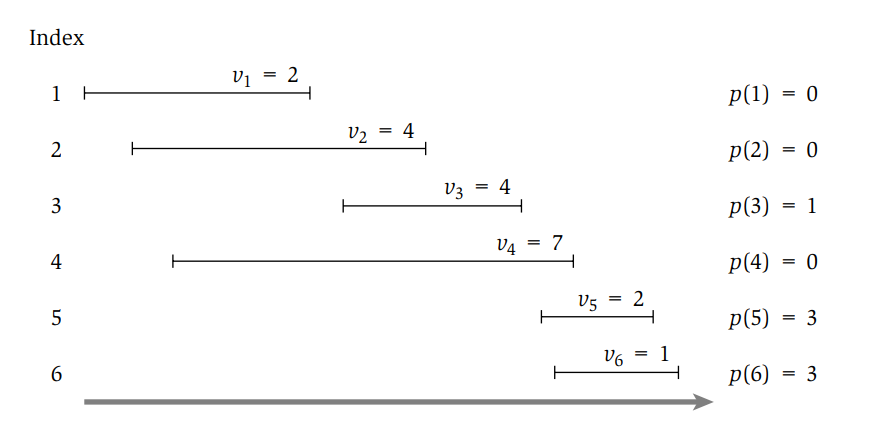
\includegraphics[width=12cm, keepaspectratio]{capitoli/imgs/weighted_problem.png}
    \caption{Istanza di un problema.}
\end{figure}

\section{Goal \normalfont{\emoji{soccer-ball}}}

L'obiettivo del nostro problema attuale è quello di trovare un sottoinsieme $S
    \subseteq \{1, \ldots, n\}$ di intervalli mutualmente compatibili che vanno a
massimizzare la somma dei pesi degli intervalli selezionati $\sum_{i \in S}
    v_i$.

\section{Funzionamento}

Come prima cosa definiamo il metodo per calcolare $OPT(j)$. Il problema è
una \textit{scelta binaria} che va a decidere se l'intervallo di indice $j$
verrà incluso nella soluzione oppure no basandosi sul valore ritornato dalla
seguente formula:

\begin{equation}
    \label{eqn:weight-opt}
    OPT(j) = max(v_j + OPT(p(j)), \ \ OPT(j-1))
\end{equation}
\ \\
Questo può essere anche visto come una disequazione:

\begin{equation}
    \label{eqn:weight-opt-dis}
    v_j + OPT(p(j)) \geq OPT(j-1)
\end{equation}
\ \\
che se vera, includerà $j$ nella soluzione ottimale.

\pagebreak

Scrivendo tutto sotto forma di algoritmo ricorsivo avremmo che:

\begin{lstlisting}[language=Javascript]
    function Compute-Opt(j){
        if (j == 0)
            return 0
        else
            return max(vj+Compute-Opt(p(j)), Compute-Opt(j − 1))
    }
\end{lstlisting}

Costruendo l'albero della ricorsione dell'algoritmo si nota che la complessità
temporale è esponenziale \emoji{astonished} !

\begin{figure}[H]
    \centering
    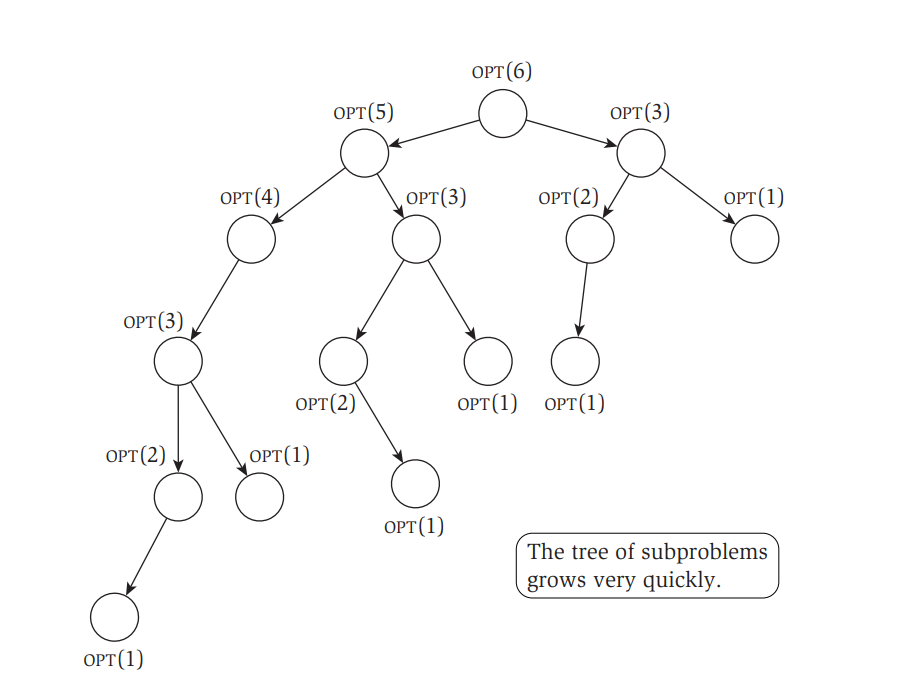
\includegraphics[width=12cm, keepaspectratio]{capitoli/imgs/opt_albero.png}
    \caption{Sviluppo dell'albero di ricorsione per la risoluzione di un problema.}
\end{figure}

\pagebreak

Una soluzione è quella di utilizzare la tecnica della \textbf{Memoization} che evita
di ricalcolare $OPT$ per gli indici già calcolati precedentemente, rendendo così
il costo temporale uguale ad $O(n)$ \emoji{man-in-motorized-wheelchair}.

\begin{lstlisting}[language=Javascript]
function M-Compute-Opt(j){
    if (j == 0)
        return 0
    else if (M[j] is not empty)
        return M[j]
    else
        let M[j] = max(vj+M-Compute-Opt(p(j)), M-Compute-Opt(j-1))
        return M[j]
}
\end{lstlisting}

Oltre al valore della soluzione ottimale probabilmente vorremmo sapere anche
quali sono gli intervalli che la compongono, e intuitivamente verrebbe da creare
un array aggiuntivo in cui verranno aggiunti gli indici degli intervalli
ottenuti con \verb|M-Compute-Opt|. Tuttavia questo aggiungerebbe una complessità
temporale di $O(n)$ peggiorando notevolmente le prestazioni. Un'alternativa è
quella di recuperare le soluzioni dai valori salvati nell'array \verb|M| dopo che la
soluzione ottimale è stata calcolata. Per farlo possiamo sfruttare la formula
vista in precedenza $v_j + OPT(p(j)) \geq OPT(j-1)$, che ci permette di
rintracciare gli intervalli della soluzione ottima.

\begin{lstlisting}[language=Javascript]
    function Find-Solution(j) {
        if (j == 0)
            Output nothing
        else if (vj + M[p(j)] >= M[j-1])
            Output j together with the result 
            of Find-Solution(p(j))
        else
            Output the result of Find-Solution(j-1)
    }
\end{lstlisting}
% \chapter{Least Squares Problem: Multi-way Choice \normalfont{\emoji{motorway}}}

Nel capitolo precedente l'algoritmo richiedeva una ricorsione basata su scelte
binarie, in questo capitolo invece introdurremo un algoritmo che richiede ad
ogni step un numero di scelte polinomiali (\textit{multi-way choice}). Vedremo
come la programmazione dinamica si presta molto bene a risolvere questi
problemi.

\section{Linear Least Square}

\subsection{Il Problema}

La formulazione del problema è la seguente:

\paragraph*{} dato un insieme $P$ composto di $n$ punti sul piano denotati con\\
$(x_1, y_1), (x_2, y_2), \ldots, (x_n, y_n)$; e supponiamo che $x_1 < x_2 <
    \ldots < x_n$ (sono strettamente crescenti). Data una linea $L$ definita
dall'equazione $y = ax + b$, definiamo l'\textit{errore} di $L$ in funzione
di $P$ come la somma delle distanze al quadrato della linea rispetto ai
punti in $P$. Formalmente:
\[
    Error(L, P) = \sum_{i=1}^{n} (y_i - ax_i - b)^2
\]

\begin{figure}[H]
    \centering
    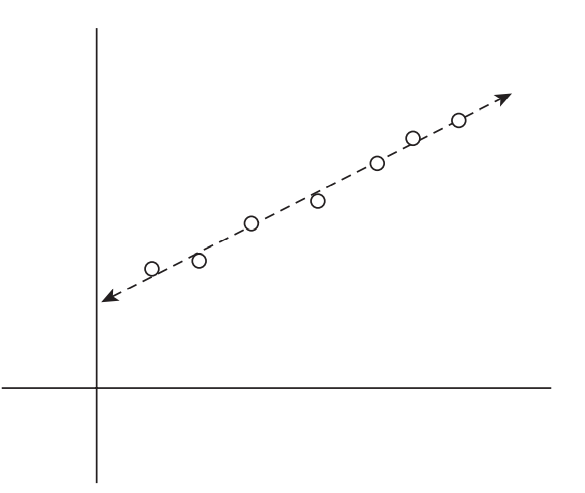
\includegraphics[width=6cm, keepaspectratio]{capitoli/imgs/linear_least.png}
    \caption{Esempio di una tipica istanza e soluzione del problema
        \textit{Linear Least}}
\end{figure}

\subsection{\goal}

È intuibile che il goal dell'algoritmo è quello di cercare la linea con errore
minimo, che può essere facilmente trovata utilizzando l'analisi matematica.
La linea di errore minimo è $y = ax + b$ dove:

\[
    a = \frac{n \sum_{i} x_i y_i - (\sum_{i} x_i) (\sum_{i} y_i)}{n \sum_{i} x_i^2 - (\sum_{i} x_i)^2} \ \ \  \ \ b = \frac{\sum_{i} y_i - a \sum_{i} x_i}{n}
\]

\section{Segmented Least Square}

Le formule appena citate sono utilizzabili solo se i punti di $P$ hanno un
andamento che è abbastanza lineare ma falliscono in altre circostanze.

\begin{figure}[H]
    \centering
    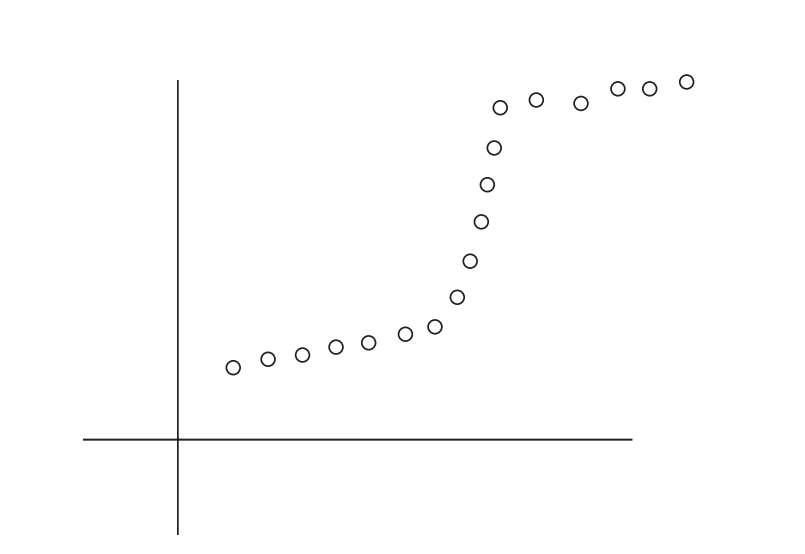
\includegraphics[width=8cm, keepaspectratio]{capitoli/imgs/segmente_linear_least.png}
    \caption{Esempio di funzione non risolvibile con Linear Least Square}
\end{figure}

Come è evidente (\textit{lapalissiano \normalfont{\emoji{gem}}}) dalla figura
non è possibile trovare una linea che approssimi in maniera soddisfacente i
punti, dunque per risolvere il problema possiamo pensare di rilassare la
condizione che sia solo una la linea. Questo però implica dover riformulare il
goal che altrimenti risulterebbe banale (si fanno $n$ linee che passano per ogni
punto).

\subsection{Costi}

La parte che computa gli errori ha costo in tempo $O(n^3)$ (si può portare a
$O(n^2)$).
La parte che trova il valore ottimo ha costo $O(n^2)$.\\

In spazio l'algoritmo ha costo $O(n^2)$ ma può essere ridotto a $O(n)$

\subsection{\goal}

Formalmente, il problema è espresso come segue:

\paragraph*{} come prima abbiamo un set di punti $P = \{(x_1, y_1), (x_2, y_2),
    \ldots, (x_n, y_n)\}$ strettamente crescenti. Denoteremo l'insieme dei punti
$(x_i, y_i)$ con $p_i$. Vogliamo partizionare $P$ in un qualche numero di
segmenti, ogni numero di segmenti è un sottoinsieme di $P$ che rappresenta un
\textit{set} contiguo delle coordinate $x$ con la forma $\{p_i, p_{i+1}, \ldots,
    p_{j-1}, p_j\}$ per degli indici $i \leq j$. Dopodiché, per ogni segmento $S$
calcoliamo la linea che minimizza l'errore rispetto ai punti in $S$ secondo
quanto espresso dalle formule enunciate prima.\\

Definiamo infine una penalità per una data partizione come la somma dei seguenti
termini:

\begin{itemize}
    \item Numero di segmenti in cui viene partizionato $P$ moltiplicato per un
          valore $C > 0$ (più è grande e più penalizza tante partizioni)
    \item Per ogni segmento l'errore della linea ottima attraverso quel
          segmento.
\end{itemize}


Il goal del Segmented Least Square Problem è quindi quello di trovare la
partizione di \textbf{penalità minima}.

\subsection{Funzionamento}

Per come è fatta la programmazione dinamica noi vogliamo suddividere il problema
in sotto-problemi e per farlo partiamo dall'osservazione che l'ultimo punto
appartiene ad una partizione ottima che parte da un valore $p_i$ fino a $p_n$ e
che possiamo togliere questi punti dal totale per ottenete un sotto-problema più
piccolo. Supponiamo che la soluzione ottima sia denotata da \verb|OPT(j)|, per i
punti che vanno da $p_1$ a $p_j$, allora avremo che la soluzione ottima al
problema dato l'ultimo segmento che va da $p_i$ a $p_n$, sarà dalla seguente
formula:

\[
    OPT(n) = e_{i,n} + C + OPT(i - 1)
\]

Questa formula è data dalla soluzione ottima dell'ultima partizione ($e_{i,n} + C$)
a cui viene aggiunta la soluzione ottima di tutte le partizioni precedenti
($OPT(i -1)$). Per i sotto-problemi possiamo scrivere la soluzione al problema
in forma ricorsiva utilizzando la formula appena espressa che prenderà la forma:

\[
    OPT(j) = \min_{1 \leq i \leq j}(e_{i,j} + C + OPT(i - 1))
\]

Possiamo ora dare una versione di questo algoritmo in pseudocodice:

\begin{lstlisting}[language=Javascript]
    function Segmented-Least-Squares(n) {
        M[0 ... n]
        M[0] = 0

        // compute the errors
        for (j in 1 ... n) {
            for (i in 1 ... j) {
                compute eij for the segment pi, ..., pj
            }
        }

        // find optimal value
        for (j in 1 ... n) {
            M[j] = min_i(eij + C + M[i - 1]) // OPT(J)
        }

        return M[n]
    }
\end{lstlisting}

Dopo aver trovato la soluzione ottima, possiamo sfruttare la memoization per
ricavarci i segmenti in tempi brevi.

\begin{lstlisting}[language=Javascript]
    function Find-Segments(j) {
        if (j == 0) print('')

        else {
            Find an i that minimizes ei,j + C + M[i − 1]
            Output the segment {pi,..., pj} and the result of Find-Segments(i − 1)
        }
    }
\end{lstlisting}

L'algoritmo ha costo $O(n^3)$ in tempo e $O(n^2)$ in spazio.
Questo tempo può essere ridotto applicando la memoization alle formule per il calcolo
dell'errore viste in precedenza portandolo a $O(n^2)$ per il tempo e $O(n)$ per lo spazio.
% \chapter{Subset Sum \& Knapsack Problem \normalfont{\emoji{money-bag}}}

\section{Il Problema}

Il problema delle Subset Sum è formalmente definito come segue:\\

\- abbiamo $n$ oggetti $\{1, \ldots, n\}$, a ognuno viene assegnato un
peso non negativo $w_i$ (per $i = 1, \ldots, n$) e ci viene dato anche un
limite $W$. L'obbiettivo è quello di selezionare un sottoinsieme $S$ degli
oggetti tale che $\sum_{i \in S}w_i \leq W$ e che questa sommatoria abbia valore
più grande possibile.\\

Questo problema è un caso specifico di un problema più generale conosciuto come
il Knapsack Problem, l'unica differenza sta nel valore da massimizzare che per il
Knapsack è un valore $v_i$ e non più il peso.

Si potrebbe pensare di risolvere questi problemi con un algoritmo greedy ma
purtroppo non ne esiste uno in grado di trovare efficientemente la soluzione ottima.
Potremmo pensare di ordinare gli oggetti in base al peso in ordine crescente o
decrescente e prenderli, tuttavia questo approccio fallisce per determinati casi
(come per l'insieme $\{W/2+1, W/2, W/2\}$ ordinato in senso decrescente) e l'unica
opzione sarà quella di provare con la programmazione dinamica \emoji{person-in-manual-wheelchair}.
\newpage

\section{\goal}

Possiamo riassumere il goal di questi problemi come segue:\\

\- Abbiamo $n$ oggetti $\{1, \ldots, n\}$, a ognuno viene assegnato un
peso non negativo $w_i$ (per $i = 1, \ldots, n$) e ci viene dato anche un
limite $W$. L'obbiettivo è quello di selezionare un sottoinsieme $S$ degli oggetti
tale che $\sum_{i \in S}w_i \leq W$ e che questa sommatoria abbia valore più
grande possibile.

\section{Costi}

\begin{center}
    \begin{tabular}{|c|c|}
        \centering
        \textbf{Funzione}    & \textbf{Costo (tempo)} \\
        \verb|Subset-Sum|    & $O(nW)$                \\
        \verb|Find-Solution| & $O(n)$                 \\
    \end{tabular}
\end{center}

\section{Funzionamento}

Come per tutti gli algoritmi dinamici dobbiamo cercare dei sotto-problemi e
possiamo utilizzare la stessa intuizione avuto per il problema dello scheduling
(scelta binaria). Facendo tutti i calcoli di dovere otteniamo la seguente
ricorsione:

\begin{center}
    se $w < w_i$ allora $OPT(i, w) = OPT(i-1,w)$ altrimenti\\
    $OPT(i, w) = max(OPT(i-1, w), w_i + OPT(i-1, w-w_i))$
\end{center}

Nella prima parte analizziamo il caso in cui l'elemento che vogliamo aggiungere va
a superare il peso massimo residuo $w$, dunque viene scartato. Nella seconda parte
andiamo ad analizzare se l'aggiunta o meno del nuovo oggetto va a migliorare
la soluzione di $OPT$ che è definita come:\\

\[
    OPT(i, w) = \max_{S} \sum_{j \in S} w_j
\]
\newpage

Possiamo formalizzare il tutto con il seguente pseudo-codice:

\begin{lstlisting}[language=JavaScript]
    function Subset-Sum(n, W) {
        let M[0 . . . n,0... W]

        //initialize the memoization vector
        for(w in 0 ... W) {
            M[0, W] = 0
        }

        //solve subproblems
        for(i in 1 ... n) {
            for(w in 0 ... W) {
                Use the recurrence to compute M[i, w]
            }
        }

        return M[n, W]
    }
\end{lstlisting}

La particolarità di questo algoritmo è che avremmo 2 insiemi di sotto-problemi
diversi che devono essere risolti per ottenere la soluzione ottima. Questo fatto
si riflette in come viene popolato l'array di memoization dei valori di $OPT$
che verranno salvati in un array bidimensionale.

\begin{figure}[H]
    \centering
    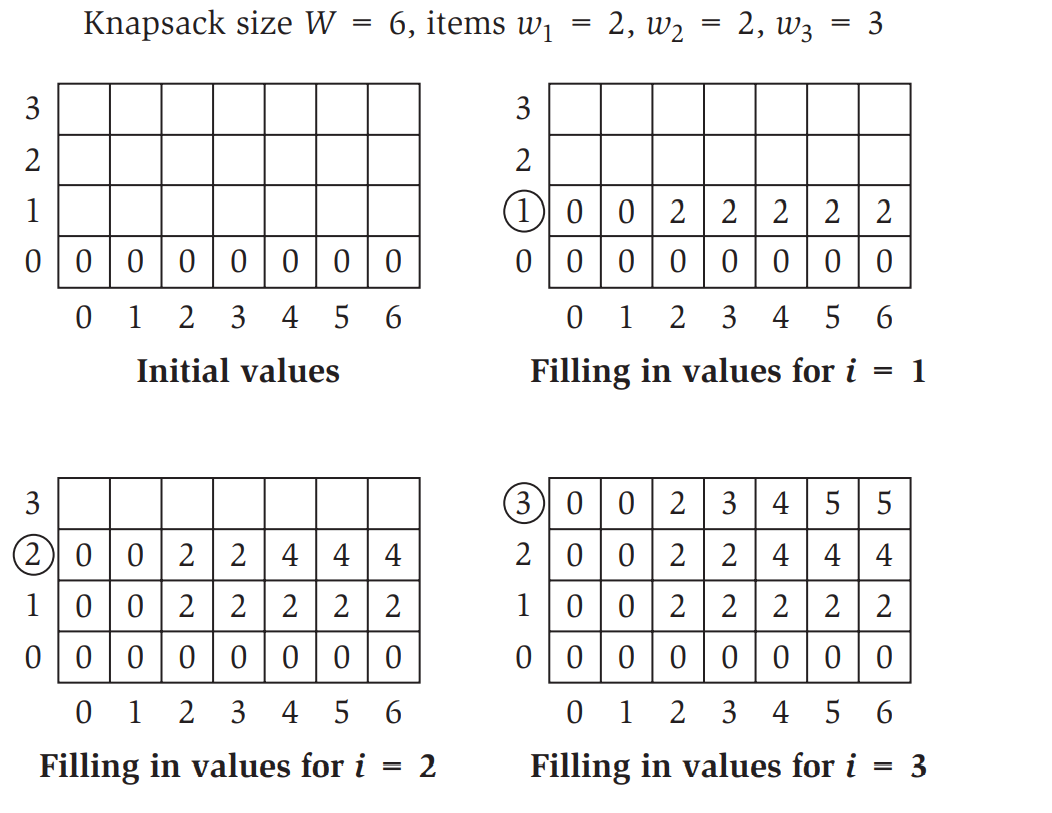
\includegraphics[width=10cm, keepaspectratio]{capitoli/imgs/knapsac_table.png}
    \caption{Esempio di come viene popolato l'array $M$ per il problema del Knapsack.}
\end{figure}

\textit{Il costo in tempo di questa implementazione è di $O(nW)$.}\\

A causa di questo costo, l'algoritmo fa parte della famiglia degli
algoritmi \textit{pseudo polinomiali}, ovvero algoritmi il cui costi dipende da
una variabile di input che se piccola, lo mantiene basso e se grande lo fa
esplodere.\\

\textit{Per recuperare gli oggetti dall'array di Memoization la complessità in tempo è di
    $O(n)$.}\\

Questa implementazione funziona anche per il problema più generale del Knapsack,
ci basterà solo cambiare la parte di ricorsione scrivendola come segue:

\begin{center}
    se $w < w_i$ allora $OPT(i, w) = OPT(i-1,w)$ altrimenti
    $OPT(i, w) = max(OPT(i-1, w), v_i + OPT(i-1, w-w_i))$
\end{center}

La complessità temporale è sempre $O(nW)$.
% \section{RNA Secondary Structure \normalfont{\emoji{dna}}}

La ricerca della struttura secondaria dell'RNA è un problema a 2 variabili
risolvibile tramite il paradigma della programmazione dinamica. Come sappiamo il
DNA è composto da due filamenti, mentre l'RNA è composto da un filamento
singolo. Questo comporta che spesso le basi di un singolo filamento di RNA si
accoppino tra di loro. L'insieme della basi può essere visto come l'alfabeto
$\{A, C, U, G\}$ e l'RNA è una sequenza di simboli presi da questo alfabeto. Il
processo di accoppiamento delle basi è dettato dalla regola di \textit{Watson-Crick} e
segue il seguente schema:

\[
    A - U \ \ \ \textrm{ e } \ \ \ C - G \ \ \ \textrm{ (l'ordine non conta)}
\]

\begin{figure}[H]
    \centering
    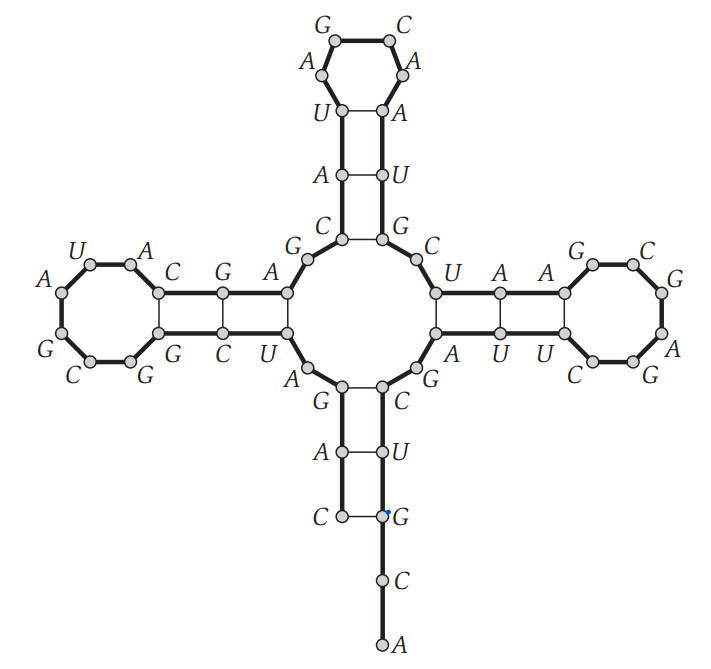
\includegraphics[width=8cm, keepaspectratio]{capitoli/dynamic_programming/imgs/rna_esempio1.png}
    \caption{Esempio di una struttura secondari di RNA} %%TODO: ricontrollare !!
\end{figure}

\subsection{Il Problema}

In questo problema si vuole trovare la struttura secondaria dell'RNA che abbia
energia libera maggiore (il maggior numero di coppie di basi possibili). Per
farlo dobbiamo tenere in considerazione alcune condizioni che devono essere
soddisfatte per permettere di approssimare al meglio il modello biologico
dell'RNA.\\

Formalmente la struttura secondaria di $B$ è un insieme di coppie $S =
    \{(i,j)\}$ dove $i,j \in \{1,2,\ldots,n\}$, che soddisfa le seguenti
condizioni:

\begin{enumerate}
    \item \textbf{No Sharp Turns}: la fine di ogni coppia è separata da almeno 4
          basi, quindi se $(i,j) \in S$ allora $i < j - 4$
    \item Gli elementi di una qualsiasi coppia $S$ consistono di $\{A, U\}$ o
          $\{C, G\}$ (in qualsiasi ordine).
    \item $S$ è un \textit{matching}: nessuna base compare in più di una coppia.
    \item \textbf{Non Crossing Condition}: se $(i, j)$ e $(k,l)$ sono due coppie
          in $S$ allora \textbf{non} può avvenire che $i < k < j < l$.
\end{enumerate}

\begin{figure}[H]
    \centering
    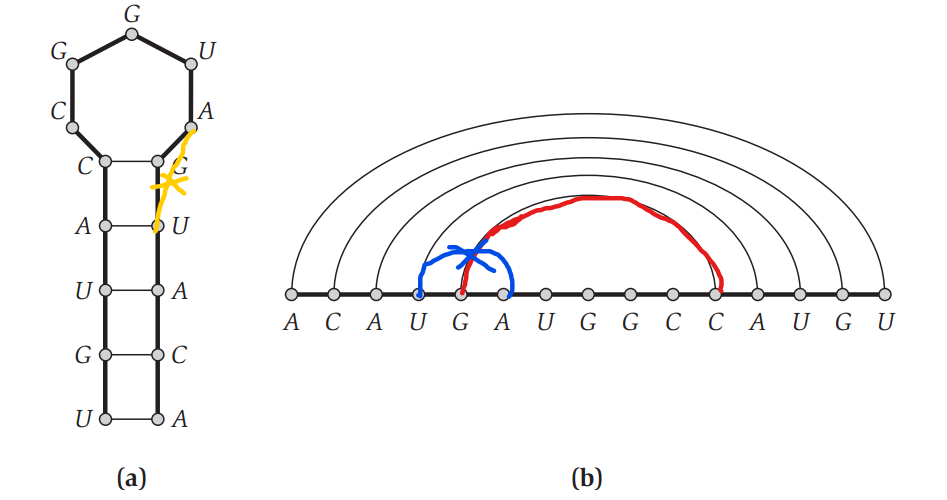
\includegraphics[width=10cm, keepaspectratio]{capitoli/dynamic_programming/imgs/rna_esempio2.png}
    \caption{La figura \textit{(a)} rappresenta un esempio di \textit{Sharp
            Turn}, mentre la figura \textit{(b)} mostra una
        \textit{Crossing Condition} dove il filo blu non dovrebbe esistere.}
\end{figure}

\subsection{\goal}

Il goal di questo problema è di massimizzare la quantità di coppie che si possono
formare all'interno della struttura secondaria di una data sequenza di RNA.

\subsection{Costi}

L'algoritmo complessivo ha costo $O(n^3)$.

\subsection{Funzionamento}

\paragraph{First Attempt.}
Come primo tentativo potremmo basarci sul seguente sotto-problema: affermiamo che
$OPT(j)$ è il massimo numero di coppie di basi sulla struttura secondaria $b_1
    b_2 \ldots b_j$, per la Non Sharp Turn Condition sappiamo che $OPT(j) = 0$ per
$j \leq 5$ e sappiamo anche che $OPT(n)$ è la soluzione che vogliamo trovare. Il
problema ora sta nell'esprimere $OPT(j)$ ricorsivamente. Possiamo parzialmente
farlo sfruttando le seguenti scelte:

\begin{itemize}
    \item $j$ non appartiene ad una coppia
    \item $j$ si accoppia con $t$ per qualche $t \leq
              j - 4$
\end{itemize}

Per il primo caso basta cercare la soluzione per $OPT(j - 1)$, nel secondo caso
invece se teniamo conto della Non Crossing Condition, possiamo isolare due nuovi
sotto-problemi: uno sulle basi $b_1 b_2 \ldots b_{t-1}$ e l'altro sulle basi
$b_{t+1} \ldots b_{j-1}$. Il primo si risolve con $OPT(t-1)$ ma il secondo, dato
che non inizia con indice $1$, non è nella lista dei nostri sotto-problemi. A
causa di ciò risulta necessario aggiungere una variabile.

\begin{figure}[H]
    \centering
    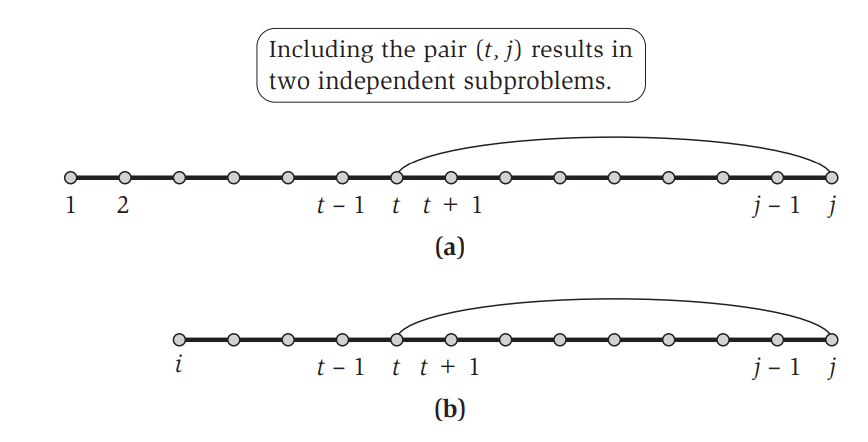
\includegraphics[width=10cm, keepaspectratio]{capitoli/dynamic_programming/imgs/rna_funzionamento.png}
    \caption{Esempio di
        utilizzo di una sola variabile \textit{(a)} o con due \textit{(b)}.}
\end{figure}

\paragraph{Dynamic Programming over Intervals}
Basandoci sui ragionamenti precedenti, possiamo scrivere una ricorsione di
successo: sia $OPT(i,j)$ il numero massimo di coppie di basi nella struttura
secondaria $b_i b_{i+1} \ldots b_j$, grazie alla non sharp turn Condition
possiamo inizializzare gli elementi con $i \geq j -4$ a $0$. Ora avremmo sempre
le stesse condizioni elencate sopra:

\begin{itemize}
    \item $j$ non appartiene ad una coppia
    \item $j$ si accoppia con $t$ per qualche $t \leq j - 4$
\end{itemize}

Nel primo caso avremmo che $OPT(i,j) = OPT(i, j-1)$, nel secondo caso possiamo
ricorrere su due sotto-problemi $OPT(i, t-1)$ e $OPT(t+1, j-1)$ affinché venga
rispettata la non crossing condition. Possiamo esprimere formalmente la
ricorsione come segue:

\begin{center}
    \[
        OPT(i, j) = \max(OPT(i, j-1), \max_t(1+OPT(i, t-1)+OPT(t+1, j-1))),
    \]
    dove il massimo è calcolato su $t$ tale che $b_t$ e $b_j$ siano una coppia di
    basi consentita
\end{center}

\begin{figure}[H]
    \centering
    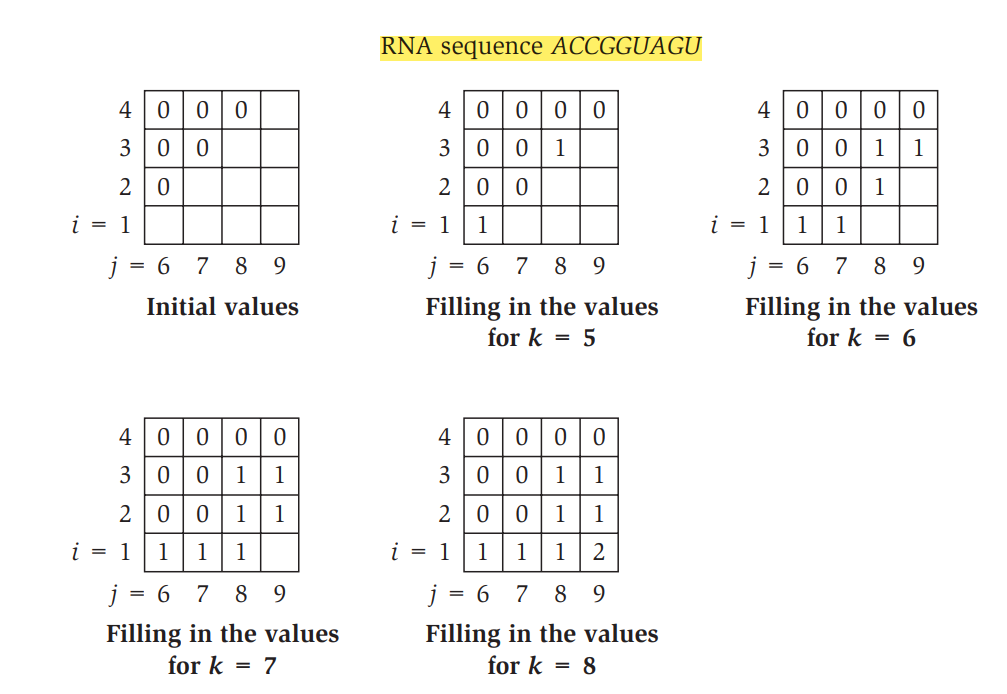
\includegraphics[width=\textwidth, keepaspectratio]{capitoli/dynamic_programming/imgs/rna_calcolo.png}
    \caption{Iterazioni dell'algoritmo su un campione del problema in questione $ACCGGUAGU$}
\end{figure}
\newpage

Possiamo infine formalizzare il tutto con il seguente pseudo-codice:

\begin{lstlisting}[language=JavaScript]
 Initialize OPT(i, j) = 0 whenever i ≥ j - 4

 for (k in 5 ... n - 1) {
     for (i in 1 ... n - k) {
         j = i + k
         Compute OPT(i, j) using the previous recurrence
     }
 }

 return OPT(1, n)
\end{lstlisting}

Ci sono $O(n^2)$ sotto-problemi da risolvere e ognuno richiede tempo $O(n)$,
quindi il running time complessivo è di $O(n^3)$.

% \section{Sequence Alignment}

Il problema del Sequence Alignment consiste nel riuscire a comparare delle
stringhe, come per esempio quando si effettua un typo in un motore di ricerca e
quello ci fornisce l'alternativa corretta. Una prima idea potrebbe essere quella
di \textbf{allineare} le due parole lettera per lettera, riempendo gli eventuali
spazi bianchi, e vedendo di quanto le due differiscono. Tuttavia ci sono varie
possibilità con cui due parole di lunghezza diversa possono essere confrontate,
quindi è necessario fornire una definizione di \textbf{similarità}.

\subsection{Il Problema}

Come prima definizione di similarità possiamo dire che minore sarà il numero di
caratteri che non corrispondono, maggiore sarà la similarità tra le parole.
Questa problematica è anche un tema centrale della biologia molecolare, e
proprio grazie ad un biologo abbiamo una definizione rigorosa e soddisfacente di
similarità. Prima di dare una definizione similarità dovremo però darne una di
\textbf{allineamento}: Supponiamo di avere due stringhe $X$ e $Y$, che consistono rispettivamente
della sequenza di simboli $x_1 x_2 \ldots x_m$ e $y_1 y_2 \ldots y_n$, e
consideriamo gli insiemi $\{1,2,\ldots ,m\}$ e $\{1,2,\ldots ,n\}$ che
rappresentano le varie posizioni nelle stringhe $X$ e $Y$, ora si considera un
\textbf{Matching} di queste due parole (un matching è stato definito nella parte
precedente e si tratta di un insieme di coppie ordinate con la proprietà che
ogni oggetto si trova al più in una sola coppia).  Diciamo ora che un matching
$M$ di questi due insiemi è un allineamento se gli elementi di varie coppie non
si incrociano: se $(i,j),(i^{\prime},j^{\prime}) \in M$  e $i < i^{\prime}$,
allora $j < j^{\prime}$.\\

Ora la nostra definizione di similarità si baserà sul trovare il miglior
allineamento, seguendo i seguenti criteri:

\begin{itemize}
    \item C'è un parametro $\delta>0$ che
          definisce la \textbf{gap penalty}, ovvero ogni volta che un simbolo di una parola
          non corrisponde ad un simbolo dell'altra.
    \item Per ogni coppia di lettere $p,q$ del
          nostro alfabeto, se c'è un accoppiamento errato si paga il corrispondente
          \textbf{mismatch cost} $a_(p,q)$.
    \item Il costo di $M$ è la somma del suo gap e mismatch
          cost, e l'obiettivo sarà quello di minimizzarlo.
\end{itemize}

\subsection{Creazione dell'algoritmo}

Ora affronteremo il problema di calcolarci questo costo minimo, e l'allineamento
ottimale che lo fornisce date le coppie $X$ e $Y$. Come al solito proveremo con
un approccio di programmazione dinamica, e per realizzare l'algoritmo
individuiamo come per altri algoritmi già visti una scelta binaria. Dato
l'allineamento ottimale $M$ allora:

\begin{itemize}
    \item $(m,n) \in M$ (quindi gli ultimi due
          simboli delle 2 stringhe sono in un matching)
    \item $(m,n) \notin M$ (gli ultimi
          simboli delle due stringhe non sono in un matching)
\end{itemize}

Tuttavia questa semplice distinzione non è sufficiente, quindi supponiamo di
aggiungere anche il seguente fatto elementare:\\

\- Sia $M$ un qualsiasi allineamento di $X$ e $Y$. se $(m,n) \notin M$, allora o
l' $m-esima$ posizione di $X$ o l' $n-esima$ posizione di $Y$ non è in un
matching di $M$.\\

Dire questo equivale a riscrivere le due condizioni sopra come tre, dunque in un
allineamento ottimo $M$ almeno una deve essere vera:

\begin{itemize}
    \item $(m,n) \in M$
    \item l'$m-esima$ posizione di $X$ non è nel matching
    \item l' $n-esima$ posizione di $Y$ non è nel matching
\end{itemize}

Ora definiamo la funzione di costo minimo $OPT(i,j)$ come costo dell'alignmet
tra $x_1 x_2 \ldots x_i$ e $y_1 y_2 \ldots y_j$. In base alle condizioni
espresse in precedenza la funzione $OPT(m,n)$ assumerà il costo relativo più
$OPT(m-1,n-1)$, in particolare (i tre casi citati sopra):

\begin{itemize}
    \item condizione 1, si
          paga un matching cost per le lettere $m,n$
    \item condizione 2 e 3, si paga un gap
          cost $\delta$ per $m$(condizione 2) o $n$(condizione 3)
\end{itemize}

Utilizzando dunque gli stessi argomenti per per i sotto problemi per
l'allineamento di costo minimo tra $X$ e $Y$ otteniamo la definizione generale
di $OPT(i,j)$:\\

L'allineamento di costo minimo soddisfa la seguente ricorsione per $i \geq 1$
e $j \geq 1$:
\[
    OPT(i,j) = min[a_{(x_i y_j)} + OPT(i-1, j-1),
            \delta + OPT(i-1, j), \delta + OPT(i, j-1)]
\]

Dunque così abbiamo ottenuto la nostra funzione di ricorsione e possiamo
procedere alla scrittura dello pseudo codice.

\begin{lstlisting}[language=JavaScript]
    function alignment(X,Y) { var A = Matrix(m, n)

        Initialize A[i, 0]= iδ for each i 
        Initialize A[0, j]= jδ for each j

        for (j in 1...n) { 
            for (i in 1...m) { 
                Use the recurrence (6.16) to compute A[i, j] 
            }
        }

        return A[m, n]
    }
\end{lstlisting}

Il running time è di $O(mn)$

\subsection{Sequence Alignment in Spazio Lineare}

Come abbiamo appena visto l'algoritmo ha sia costo spaziale che temporale uguale
a $O(mn)$ e se come input consideriamo le parole della lingua inglese non
risulta essere un grande problema, ma se consideriamo genomi con 10 miliardi di
caratteri potrebbe risultare difficile poter lavorare con array di 10 GB \emoji{astonished}.
Questo problema può essere risolto utilizzando un approccio \textit{divide et impera}
che va a rendere lineare il costo dello spazio ( $O(n + m)$ ).

\subsubsection{Funzionamento}

Come prima cosa definiamo un algoritmo Space Efficient Alignment che ci permette
di trovare la soluzione ottima utilizzando il minor spazio possibile. Per farlo
notiamo che la funzione $OPT$ dipende solamente da una colonna precedente di
quella che si sta analizzando, dunque basterà caricarsi in memoria una matrice
$mx2$ riducendo così il costo spaziale ad $m$. Tuttavia utilizzando questo
metodo non e possibile ricurvare l'alignment effettivo perché non ci bastano le
informazioni.\\

Lo pseudo-codice dell'algoritmo appena definito è il seguente:

\begin{lstlisting}[language=JavaScript]
    function Space-Efficient-Alignment(X,Y) {
        var B = Matrix(m, 2)

        // (just as in column 0 of A)
        Initialize B[i, 0]= iδ for each i 

        for (j in 1...n) {
            B[0, 1]= jδ (since this corresponds to entry A[0, j])

            for (i in 1...m) {
                B[i, 1]= min[
                    αxiyj + B[i − 1, 0],
                    δ + B[i − 1, 1], 
                    δ + B[i, 0]
                ]
            }

            Move column 1 of B to column 0 to make room 
            for next iteration:
            Update B[i, 0] = B[i, 1] for each i
        }
    }
\end{lstlisting}

Possiamo quindi utilizzare un approccio \textit{divide et impera} che incorpora 2
tecniche diverse di programmazione dinamica per sfruttare questo approccio
appena definito e riuscire a trovare anche l'alignment in spazio lineare.
Definiamo quindi due funzioni:

\begin{itemize}
    \item $f(i, j)$ : è la funzione definita per l'algoritmo di Sequence
          Alignment di base (analoga a $OPT(i,j)$ )
    \item $g(i, j)$ : è l'analogo al contrario di $f$ ed è definito dalla
          seguente funzione ricorsiva: per $i < m$ e $j < n$ : $g(i,j) =
              min[a_{x+1y+1} + g(i+1, j+1), \delta + g(i, j+1), \delta + g(i+1, j)]$
\end{itemize}

Possiamo notare che la ricorsione $f$ procede a ritroso partendo dal fondo
mentre la ricorsione $g$ procede in avanti partendo dall'inizio. Possiamo
sfruttare questo fatto per provare ad utilizzare lo Space Efficiente Sequence
Alignment Algorithm combinato ad un approccio \textit{divide et impera} e un array di
supporto $P$ per riuscire a calcolare il Sequence Alignment in spazio lineare,
aumentando solo di una costatane la complessità temporale.\\

Possiamo riassumere il tutto con il seguente pseudo-codice:

\begin{lstlisting}[language=JavaScript]
    function Divide-and-Conquer-Alignment(X,Y) {
        var m = length(X)
        var n = length(Y)

        if (m <= 2 or n <= 2) {
            Compute optimal alignment using Alignment(X,Y)
        }

        Space-Efficient-Alignment(X, Y[1 : n/2])
        Backward-Space-Efficient-Alignment(X, Y[n/2 + 1 : n])

        Let q be the index minimizing f(q, n/2) + g(q, n/2)
        Add (q, n/2) to global list P

        Divide-and-Conquer-Alignment(X[1 : q],Y[1 : n/2])
        Divide-and-Conquer-Alignment(X[q + 1 : n],Y[n/2 + 1:n])

        return P
    }
\end{lstlisting}

\begin{figure}[H]
    \centering
    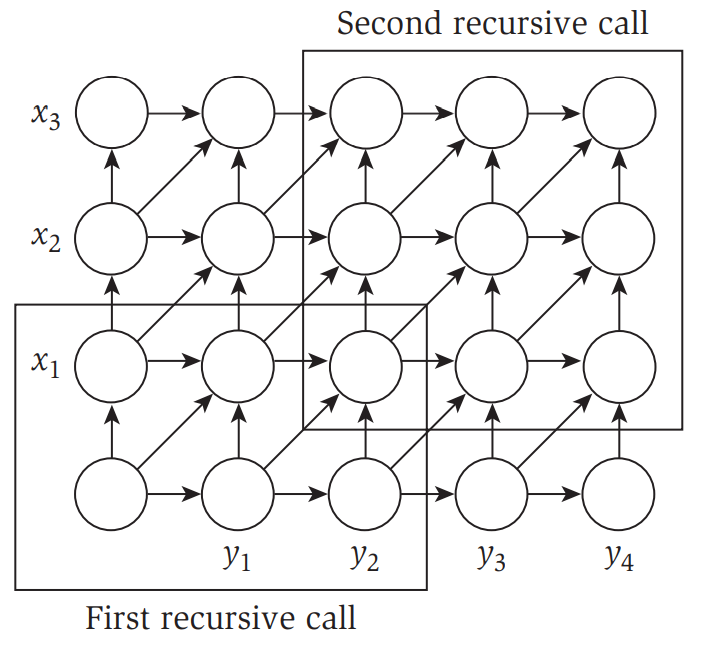
\includegraphics[width=8cm, keepaspectratio]{capitoli/dynamic_programming/imgs/seq_align_recurrence.png}
    \caption{La figura mostra il funzionamento dell'algoritmo appena descritto.}
\end{figure}

\documentclass[a4paper,12 pt]{report}
\usepackage[T1]{fontenc}
\usepackage[utf8]{inputenc}
% \usepackage{amsmath}
\usepackage{lmodern}
\usepackage{listings}
\usepackage{graphicx}
\usepackage{float}
\usepackage{subcaption}
\usepackage{hyperref}
\usepackage{wrapfig}
\usepackage{fancyhdr}
% \usepackage{tcolorbox}

% forza le footnote a stare il più in basso possibile
\usepackage[bottom]{footmisc}
\usepackage{enumitem}

%% STILE LISTINGS

\usepackage{xcolor}

\definecolor{codegreen}{rgb}{0,0.6,0}
\definecolor{codegray}{rgb}{0.5,0.5,0.5}
\definecolor{codepurple}{rgb}{0.58,0,0.82}
\definecolor{backcolour}{rgb}{0.95,0.95,0.92}

\lstdefinestyle{mystyle}{
    backgroundcolor=\color{backcolour},   
    commentstyle=\color{codegreen},
    keywordstyle=\color{magenta},
    numberstyle=\tiny\color{codegray},
    stringstyle=\color{codepurple},
    basicstyle=\ttfamily\footnotesize,
    breakatwhitespace=false,         
    breaklines=true,                 
    captionpos=b,                    
    keepspaces=true,                 
    numbers=left,                    
    numbersep=5pt,                  
    showspaces=false,                
    showstringspaces=false,
    showtabs=false,                  
    tabsize=2
}

\lstset{style=mystyle}

%% SOLIDITY Settings

% Copyright 2017 Sergei Tikhomirov, MIT License
% https://github.com/s-tikhomirov/solidity-latex-highlighting/

%\usepackage{listings, xcolor}

\definecolor{verylightgray}{rgb}{.97,.97,.97}

\lstdefinelanguage{Solidity}{
	keywords=[1]{anonymous, assembly, assert, balance, break, call, callcode, case, catch, class, constant, continue, constructor, contract, debugger, default, delegatecall, delete, do, else, emit, event, experimental, export, external, false, finally, for, function, gas, if, implements, import, in, indexed, instanceof, interface, internal, is, length, library, log0, log1, log2, log3, log4, memory, modifier, new, payable, pragma, private, protected, public, pure, push, require, return, returns, revert, selfdestruct, send, solidity, storage, struct, suicide, super, switch, then, this, throw, transfer, true, try, typeof, using, value, view, while, with, addmod, ecrecover, keccak256, mulmod, ripemd160, sha256, sha3}, % generic keywords including crypto operations
	keywordstyle=[1]\color{blue}\bfseries,
	keywords=[2]{address, bool, byte, bytes, bytes1, bytes2, bytes3, bytes4, bytes5, bytes6, bytes7, bytes8, bytes9, bytes10, bytes11, bytes12, bytes13, bytes14, bytes15, bytes16, bytes17, bytes18, bytes19, bytes20, bytes21, bytes22, bytes23, bytes24, bytes25, bytes26, bytes27, bytes28, bytes29, bytes30, bytes31, bytes32, enum, int, int8, int16, int24, int32, int40, int48, int56, int64, int72, int80, int88, int96, int104, int112, int120, int128, int136, int144, int152, int160, int168, int176, int184, int192, int200, int208, int216, int224, int232, int240, int248, int256, mapping, string, uint, uint8, uint16, uint24, uint32, uint40, uint48, uint56, uint64, uint72, uint80, uint88, uint96, uint104, uint112, uint120, uint128, uint136, uint144, uint152, uint160, uint168, uint176, uint184, uint192, uint200, uint208, uint216, uint224, uint232, uint240, uint248, uint256, var, void, ether, finney, szabo, wei, days, hours, minutes, seconds, weeks, years},	% types; money and time units
	keywordstyle=[2]\color{teal}\bfseries,
	keywords=[3]{block, blockhash, coinbase, difficulty, gaslimit, number, timestamp, msg, data, gas, sender, sig, value, now, tx, gasprice, origin},	% environment variables
	keywordstyle=[3]\color{violet}\bfseries,
	identifierstyle=\color{black},
	sensitive=false,
	comment=[l]{//},
	morecomment=[s]{/*}{*/},
	commentstyle=\color{gray}\ttfamily,
	stringstyle=\color{red}\ttfamily,
	morestring=[b]',
	morestring=[b]"
}

\lstdefinelanguage{JavaScript}{
  keywords={typeof, new, true, false, catch, function, return, null, catch, switch, var, if, in, while, do, else, case, break},
  keywordstyle=\color{blue}\bfseries,
  ndkeywords={class, export, boolean, throw, implements, import, this},
  ndkeywordstyle=\color{darkgray}\bfseries,
  identifierstyle=\color{black},
  sensitive=false,
  comment=[l]{//},
  morecomment=[s]{/*}{*/},
  commentstyle=\color{purple}\ttfamily,
  stringstyle=\color{red}\ttfamily,
  morestring=[b]',
  morestring=[b]"
}
%\lstset{
%	language=Solidity,
%	backgroundcolor=\color{verylightgray},
%	extendedchars=true,
%	basicstyle=\footnotesize\ttfamily,
%	showstringspaces=false,
%	showspaces=false,
%	numbers=left,
%	numberstyle=\footnotesize,
%	numbersep=9pt,
%	tabsize=2,
%	breaklines=true,
%	showtabs=false,
%	captionpos=b
%}

%% -----

% box around text
\newenvironment{boxed}
    {\begin{center}
    \begin{tabular}{|p{\textwidth}|}
    \hline\\
    }
    { 
    \\\\\hline
    \end{tabular} 
    \end{center}
    }

% Resetta la numerazione dei chapter quando
% una nuova part viene creata
\makeatletter
\@addtoreset{chapter}{part}
\makeatother

% Rimuove l'indentazione quando si crea un nuovo paragrafo
\setlength{\parindent}{0pt}

% footer
\pagestyle{fancyplain}
% rimuove la riga nell'header
\fancyhf{} % sets both header and footer to nothing
\renewcommand{\headrulewidth}{0pt}
\fancyfoot[L]{\href{https://github.com/Typing-Monkeys/AppuntiUniversita}{Typing Monkeys}}
\fancyfoot[C]{\emoji{gorilla}}
\fancyfoot[R]{\thepage}

% configurazione emoji
\usepackage{fontspec}
\usepackage{emoji}
\setemojifont{NotoColorEmoji.ttf}[Path=/usr/share/fonts/truetype/noto/]


% Macro
\newcommand{\goal}{Goal \normalfont{\emoji{soccer-ball}}}


\begin{document}
\include{frontmatter/main.tex}

%% TODO: riorganizzare la struttura degli appunti
%%       alla fine dovremmo avere una roba del tipo
%%          - Programmazione Dinamica
%%            - Arg 1
%%            - Arg 2
%%              - subarg 1
%%              - subarg 2
%%          - Flow
%%            - Arg 1
%%              - sub arg 1
%%          - Graph
%%            - Arg 1
%%

\tableofcontents

\include{quote/main.tex}

% \include{capitoli/dynamic_programming/1-introduzione_all_programmazione_dinamica.tex}
% \include{capitoli/dynamic_programming/2-weighted_interval_scheduling.tex}
% \include{capitoli/dynamic_programming/3-least_squares_problem_multiway_choice.tex}
% \include{capitoli/dynamic_programming/4-subset_sum_e_knapsack_problem.tex}
% \include{capitoli/dynamic_programming/5-rna_secondary_structure.tex}
% \include{capitoli/dynamic_programming/6-sequence_alignment.tex}
\include{capitoli/dynamic_programming/main.tex}

\end{document}

\end{document}

\end{document}

%% TODO: riorganizzare la struttura degli appunti
%%       alla fine dovremmo avere una roba del tipo
%%          - Programmazione Dinamica
%%            - Arg 1
%%            - Arg 2
%%              - subarg 1
%%              - subarg 2
%%          - Flow
%%            - Arg 1
%%              - sub arg 1
%%          - Graph
%%            - Arg 1
%%

\tableofcontents

\documentclass[a4paper,12 pt]{report}
\usepackage[T1]{fontenc}
\usepackage[utf8]{inputenc}
% \usepackage{amsmath}
\usepackage{lmodern}
\usepackage{listings}
\usepackage{graphicx}
\usepackage{float}
\usepackage{subcaption}
\usepackage{hyperref}
\usepackage{wrapfig}
\usepackage{fancyhdr}
% \usepackage{tcolorbox}

% forza le footnote a stare il più in basso possibile
\usepackage[bottom]{footmisc}
\usepackage{enumitem}

%% STILE LISTINGS

\usepackage{xcolor}

\definecolor{codegreen}{rgb}{0,0.6,0}
\definecolor{codegray}{rgb}{0.5,0.5,0.5}
\definecolor{codepurple}{rgb}{0.58,0,0.82}
\definecolor{backcolour}{rgb}{0.95,0.95,0.92}

\lstdefinestyle{mystyle}{
    backgroundcolor=\color{backcolour},   
    commentstyle=\color{codegreen},
    keywordstyle=\color{magenta},
    numberstyle=\tiny\color{codegray},
    stringstyle=\color{codepurple},
    basicstyle=\ttfamily\footnotesize,
    breakatwhitespace=false,         
    breaklines=true,                 
    captionpos=b,                    
    keepspaces=true,                 
    numbers=left,                    
    numbersep=5pt,                  
    showspaces=false,                
    showstringspaces=false,
    showtabs=false,                  
    tabsize=2
}

\lstset{style=mystyle}

%% SOLIDITY Settings

% Copyright 2017 Sergei Tikhomirov, MIT License
% https://github.com/s-tikhomirov/solidity-latex-highlighting/

%\usepackage{listings, xcolor}

\definecolor{verylightgray}{rgb}{.97,.97,.97}

\lstdefinelanguage{Solidity}{
	keywords=[1]{anonymous, assembly, assert, balance, break, call, callcode, case, catch, class, constant, continue, constructor, contract, debugger, default, delegatecall, delete, do, else, emit, event, experimental, export, external, false, finally, for, function, gas, if, implements, import, in, indexed, instanceof, interface, internal, is, length, library, log0, log1, log2, log3, log4, memory, modifier, new, payable, pragma, private, protected, public, pure, push, require, return, returns, revert, selfdestruct, send, solidity, storage, struct, suicide, super, switch, then, this, throw, transfer, true, try, typeof, using, value, view, while, with, addmod, ecrecover, keccak256, mulmod, ripemd160, sha256, sha3}, % generic keywords including crypto operations
	keywordstyle=[1]\color{blue}\bfseries,
	keywords=[2]{address, bool, byte, bytes, bytes1, bytes2, bytes3, bytes4, bytes5, bytes6, bytes7, bytes8, bytes9, bytes10, bytes11, bytes12, bytes13, bytes14, bytes15, bytes16, bytes17, bytes18, bytes19, bytes20, bytes21, bytes22, bytes23, bytes24, bytes25, bytes26, bytes27, bytes28, bytes29, bytes30, bytes31, bytes32, enum, int, int8, int16, int24, int32, int40, int48, int56, int64, int72, int80, int88, int96, int104, int112, int120, int128, int136, int144, int152, int160, int168, int176, int184, int192, int200, int208, int216, int224, int232, int240, int248, int256, mapping, string, uint, uint8, uint16, uint24, uint32, uint40, uint48, uint56, uint64, uint72, uint80, uint88, uint96, uint104, uint112, uint120, uint128, uint136, uint144, uint152, uint160, uint168, uint176, uint184, uint192, uint200, uint208, uint216, uint224, uint232, uint240, uint248, uint256, var, void, ether, finney, szabo, wei, days, hours, minutes, seconds, weeks, years},	% types; money and time units
	keywordstyle=[2]\color{teal}\bfseries,
	keywords=[3]{block, blockhash, coinbase, difficulty, gaslimit, number, timestamp, msg, data, gas, sender, sig, value, now, tx, gasprice, origin},	% environment variables
	keywordstyle=[3]\color{violet}\bfseries,
	identifierstyle=\color{black},
	sensitive=false,
	comment=[l]{//},
	morecomment=[s]{/*}{*/},
	commentstyle=\color{gray}\ttfamily,
	stringstyle=\color{red}\ttfamily,
	morestring=[b]',
	morestring=[b]"
}

\lstdefinelanguage{JavaScript}{
  keywords={typeof, new, true, false, catch, function, return, null, catch, switch, var, if, in, while, do, else, case, break},
  keywordstyle=\color{blue}\bfseries,
  ndkeywords={class, export, boolean, throw, implements, import, this},
  ndkeywordstyle=\color{darkgray}\bfseries,
  identifierstyle=\color{black},
  sensitive=false,
  comment=[l]{//},
  morecomment=[s]{/*}{*/},
  commentstyle=\color{purple}\ttfamily,
  stringstyle=\color{red}\ttfamily,
  morestring=[b]',
  morestring=[b]"
}
%\lstset{
%	language=Solidity,
%	backgroundcolor=\color{verylightgray},
%	extendedchars=true,
%	basicstyle=\footnotesize\ttfamily,
%	showstringspaces=false,
%	showspaces=false,
%	numbers=left,
%	numberstyle=\footnotesize,
%	numbersep=9pt,
%	tabsize=2,
%	breaklines=true,
%	showtabs=false,
%	captionpos=b
%}

%% -----

% box around text
\newenvironment{boxed}
    {\begin{center}
    \begin{tabular}{|p{\textwidth}|}
    \hline\\
    }
    { 
    \\\\\hline
    \end{tabular} 
    \end{center}
    }

% Resetta la numerazione dei chapter quando
% una nuova part viene creata
\makeatletter
\@addtoreset{chapter}{part}
\makeatother

% Rimuove l'indentazione quando si crea un nuovo paragrafo
\setlength{\parindent}{0pt}

% footer
\pagestyle{fancyplain}
% rimuove la riga nell'header
\fancyhf{} % sets both header and footer to nothing
\renewcommand{\headrulewidth}{0pt}
\fancyfoot[L]{\href{https://github.com/Typing-Monkeys/AppuntiUniversita}{Typing Monkeys}}
\fancyfoot[C]{\emoji{gorilla}}
\fancyfoot[R]{\thepage}

% configurazione emoji
\usepackage{fontspec}
\usepackage{emoji}
\setemojifont{NotoColorEmoji.ttf}[Path=/usr/share/fonts/truetype/noto/]


% Macro
\newcommand{\goal}{Goal \normalfont{\emoji{soccer-ball}}}


\begin{document}
\documentclass[a4paper,12 pt]{report}
\usepackage[T1]{fontenc}
\usepackage[utf8]{inputenc}
% \usepackage{amsmath}
\usepackage{lmodern}
\usepackage{listings}
\usepackage{graphicx}
\usepackage{float}
\usepackage{subcaption}
\usepackage{hyperref}
\usepackage{wrapfig}
\usepackage{fancyhdr}
% \usepackage{tcolorbox}

% forza le footnote a stare il più in basso possibile
\usepackage[bottom]{footmisc}
\usepackage{enumitem}

%% STILE LISTINGS

\usepackage{xcolor}

\definecolor{codegreen}{rgb}{0,0.6,0}
\definecolor{codegray}{rgb}{0.5,0.5,0.5}
\definecolor{codepurple}{rgb}{0.58,0,0.82}
\definecolor{backcolour}{rgb}{0.95,0.95,0.92}

\lstdefinestyle{mystyle}{
    backgroundcolor=\color{backcolour},   
    commentstyle=\color{codegreen},
    keywordstyle=\color{magenta},
    numberstyle=\tiny\color{codegray},
    stringstyle=\color{codepurple},
    basicstyle=\ttfamily\footnotesize,
    breakatwhitespace=false,         
    breaklines=true,                 
    captionpos=b,                    
    keepspaces=true,                 
    numbers=left,                    
    numbersep=5pt,                  
    showspaces=false,                
    showstringspaces=false,
    showtabs=false,                  
    tabsize=2
}

\lstset{style=mystyle}

%% SOLIDITY Settings

% Copyright 2017 Sergei Tikhomirov, MIT License
% https://github.com/s-tikhomirov/solidity-latex-highlighting/

%\usepackage{listings, xcolor}

\definecolor{verylightgray}{rgb}{.97,.97,.97}

\lstdefinelanguage{Solidity}{
	keywords=[1]{anonymous, assembly, assert, balance, break, call, callcode, case, catch, class, constant, continue, constructor, contract, debugger, default, delegatecall, delete, do, else, emit, event, experimental, export, external, false, finally, for, function, gas, if, implements, import, in, indexed, instanceof, interface, internal, is, length, library, log0, log1, log2, log3, log4, memory, modifier, new, payable, pragma, private, protected, public, pure, push, require, return, returns, revert, selfdestruct, send, solidity, storage, struct, suicide, super, switch, then, this, throw, transfer, true, try, typeof, using, value, view, while, with, addmod, ecrecover, keccak256, mulmod, ripemd160, sha256, sha3}, % generic keywords including crypto operations
	keywordstyle=[1]\color{blue}\bfseries,
	keywords=[2]{address, bool, byte, bytes, bytes1, bytes2, bytes3, bytes4, bytes5, bytes6, bytes7, bytes8, bytes9, bytes10, bytes11, bytes12, bytes13, bytes14, bytes15, bytes16, bytes17, bytes18, bytes19, bytes20, bytes21, bytes22, bytes23, bytes24, bytes25, bytes26, bytes27, bytes28, bytes29, bytes30, bytes31, bytes32, enum, int, int8, int16, int24, int32, int40, int48, int56, int64, int72, int80, int88, int96, int104, int112, int120, int128, int136, int144, int152, int160, int168, int176, int184, int192, int200, int208, int216, int224, int232, int240, int248, int256, mapping, string, uint, uint8, uint16, uint24, uint32, uint40, uint48, uint56, uint64, uint72, uint80, uint88, uint96, uint104, uint112, uint120, uint128, uint136, uint144, uint152, uint160, uint168, uint176, uint184, uint192, uint200, uint208, uint216, uint224, uint232, uint240, uint248, uint256, var, void, ether, finney, szabo, wei, days, hours, minutes, seconds, weeks, years},	% types; money and time units
	keywordstyle=[2]\color{teal}\bfseries,
	keywords=[3]{block, blockhash, coinbase, difficulty, gaslimit, number, timestamp, msg, data, gas, sender, sig, value, now, tx, gasprice, origin},	% environment variables
	keywordstyle=[3]\color{violet}\bfseries,
	identifierstyle=\color{black},
	sensitive=false,
	comment=[l]{//},
	morecomment=[s]{/*}{*/},
	commentstyle=\color{gray}\ttfamily,
	stringstyle=\color{red}\ttfamily,
	morestring=[b]',
	morestring=[b]"
}

\lstdefinelanguage{JavaScript}{
  keywords={typeof, new, true, false, catch, function, return, null, catch, switch, var, if, in, while, do, else, case, break},
  keywordstyle=\color{blue}\bfseries,
  ndkeywords={class, export, boolean, throw, implements, import, this},
  ndkeywordstyle=\color{darkgray}\bfseries,
  identifierstyle=\color{black},
  sensitive=false,
  comment=[l]{//},
  morecomment=[s]{/*}{*/},
  commentstyle=\color{purple}\ttfamily,
  stringstyle=\color{red}\ttfamily,
  morestring=[b]',
  morestring=[b]"
}
%\lstset{
%	language=Solidity,
%	backgroundcolor=\color{verylightgray},
%	extendedchars=true,
%	basicstyle=\footnotesize\ttfamily,
%	showstringspaces=false,
%	showspaces=false,
%	numbers=left,
%	numberstyle=\footnotesize,
%	numbersep=9pt,
%	tabsize=2,
%	breaklines=true,
%	showtabs=false,
%	captionpos=b
%}

%% -----

% box around text
\newenvironment{boxed}
    {\begin{center}
    \begin{tabular}{|p{\textwidth}|}
    \hline\\
    }
    { 
    \\\\\hline
    \end{tabular} 
    \end{center}
    }

% Resetta la numerazione dei chapter quando
% una nuova part viene creata
\makeatletter
\@addtoreset{chapter}{part}
\makeatother

% Rimuove l'indentazione quando si crea un nuovo paragrafo
\setlength{\parindent}{0pt}

% footer
\pagestyle{fancyplain}
% rimuove la riga nell'header
\fancyhf{} % sets both header and footer to nothing
\renewcommand{\headrulewidth}{0pt}
\fancyfoot[L]{\href{https://github.com/Typing-Monkeys/AppuntiUniversita}{Typing Monkeys}}
\fancyfoot[C]{\emoji{gorilla}}
\fancyfoot[R]{\thepage}

% configurazione emoji
\usepackage{fontspec}
\usepackage{emoji}
\setemojifont{NotoColorEmoji.ttf}[Path=/usr/share/fonts/truetype/noto/]


% Macro
\newcommand{\goal}{Goal \normalfont{\emoji{soccer-ball}}}


\begin{document}
\documentclass[a4paper,12 pt]{report}
\usepackage[T1]{fontenc}
\usepackage[utf8]{inputenc}
% \usepackage{amsmath}
\usepackage{lmodern}
\usepackage{listings}
\usepackage{graphicx}
\usepackage{float}
\usepackage{subcaption}
\usepackage{hyperref}
\usepackage{wrapfig}
\usepackage{fancyhdr}
% \usepackage{tcolorbox}

% forza le footnote a stare il più in basso possibile
\usepackage[bottom]{footmisc}
\usepackage{enumitem}

%% STILE LISTINGS

\usepackage{xcolor}

\definecolor{codegreen}{rgb}{0,0.6,0}
\definecolor{codegray}{rgb}{0.5,0.5,0.5}
\definecolor{codepurple}{rgb}{0.58,0,0.82}
\definecolor{backcolour}{rgb}{0.95,0.95,0.92}

\lstdefinestyle{mystyle}{
    backgroundcolor=\color{backcolour},   
    commentstyle=\color{codegreen},
    keywordstyle=\color{magenta},
    numberstyle=\tiny\color{codegray},
    stringstyle=\color{codepurple},
    basicstyle=\ttfamily\footnotesize,
    breakatwhitespace=false,         
    breaklines=true,                 
    captionpos=b,                    
    keepspaces=true,                 
    numbers=left,                    
    numbersep=5pt,                  
    showspaces=false,                
    showstringspaces=false,
    showtabs=false,                  
    tabsize=2
}

\lstset{style=mystyle}

%% SOLIDITY Settings

% Copyright 2017 Sergei Tikhomirov, MIT License
% https://github.com/s-tikhomirov/solidity-latex-highlighting/

%\usepackage{listings, xcolor}

\definecolor{verylightgray}{rgb}{.97,.97,.97}

\lstdefinelanguage{Solidity}{
	keywords=[1]{anonymous, assembly, assert, balance, break, call, callcode, case, catch, class, constant, continue, constructor, contract, debugger, default, delegatecall, delete, do, else, emit, event, experimental, export, external, false, finally, for, function, gas, if, implements, import, in, indexed, instanceof, interface, internal, is, length, library, log0, log1, log2, log3, log4, memory, modifier, new, payable, pragma, private, protected, public, pure, push, require, return, returns, revert, selfdestruct, send, solidity, storage, struct, suicide, super, switch, then, this, throw, transfer, true, try, typeof, using, value, view, while, with, addmod, ecrecover, keccak256, mulmod, ripemd160, sha256, sha3}, % generic keywords including crypto operations
	keywordstyle=[1]\color{blue}\bfseries,
	keywords=[2]{address, bool, byte, bytes, bytes1, bytes2, bytes3, bytes4, bytes5, bytes6, bytes7, bytes8, bytes9, bytes10, bytes11, bytes12, bytes13, bytes14, bytes15, bytes16, bytes17, bytes18, bytes19, bytes20, bytes21, bytes22, bytes23, bytes24, bytes25, bytes26, bytes27, bytes28, bytes29, bytes30, bytes31, bytes32, enum, int, int8, int16, int24, int32, int40, int48, int56, int64, int72, int80, int88, int96, int104, int112, int120, int128, int136, int144, int152, int160, int168, int176, int184, int192, int200, int208, int216, int224, int232, int240, int248, int256, mapping, string, uint, uint8, uint16, uint24, uint32, uint40, uint48, uint56, uint64, uint72, uint80, uint88, uint96, uint104, uint112, uint120, uint128, uint136, uint144, uint152, uint160, uint168, uint176, uint184, uint192, uint200, uint208, uint216, uint224, uint232, uint240, uint248, uint256, var, void, ether, finney, szabo, wei, days, hours, minutes, seconds, weeks, years},	% types; money and time units
	keywordstyle=[2]\color{teal}\bfseries,
	keywords=[3]{block, blockhash, coinbase, difficulty, gaslimit, number, timestamp, msg, data, gas, sender, sig, value, now, tx, gasprice, origin},	% environment variables
	keywordstyle=[3]\color{violet}\bfseries,
	identifierstyle=\color{black},
	sensitive=false,
	comment=[l]{//},
	morecomment=[s]{/*}{*/},
	commentstyle=\color{gray}\ttfamily,
	stringstyle=\color{red}\ttfamily,
	morestring=[b]',
	morestring=[b]"
}

\lstdefinelanguage{JavaScript}{
  keywords={typeof, new, true, false, catch, function, return, null, catch, switch, var, if, in, while, do, else, case, break},
  keywordstyle=\color{blue}\bfseries,
  ndkeywords={class, export, boolean, throw, implements, import, this},
  ndkeywordstyle=\color{darkgray}\bfseries,
  identifierstyle=\color{black},
  sensitive=false,
  comment=[l]{//},
  morecomment=[s]{/*}{*/},
  commentstyle=\color{purple}\ttfamily,
  stringstyle=\color{red}\ttfamily,
  morestring=[b]',
  morestring=[b]"
}
%\lstset{
%	language=Solidity,
%	backgroundcolor=\color{verylightgray},
%	extendedchars=true,
%	basicstyle=\footnotesize\ttfamily,
%	showstringspaces=false,
%	showspaces=false,
%	numbers=left,
%	numberstyle=\footnotesize,
%	numbersep=9pt,
%	tabsize=2,
%	breaklines=true,
%	showtabs=false,
%	captionpos=b
%}

%% -----

% box around text
\newenvironment{boxed}
    {\begin{center}
    \begin{tabular}{|p{\textwidth}|}
    \hline\\
    }
    { 
    \\\\\hline
    \end{tabular} 
    \end{center}
    }

% Resetta la numerazione dei chapter quando
% una nuova part viene creata
\makeatletter
\@addtoreset{chapter}{part}
\makeatother

% Rimuove l'indentazione quando si crea un nuovo paragrafo
\setlength{\parindent}{0pt}

% footer
\pagestyle{fancyplain}
% rimuove la riga nell'header
\fancyhf{} % sets both header and footer to nothing
\renewcommand{\headrulewidth}{0pt}
\fancyfoot[L]{\href{https://github.com/Typing-Monkeys/AppuntiUniversita}{Typing Monkeys}}
\fancyfoot[C]{\emoji{gorilla}}
\fancyfoot[R]{\thepage}

% configurazione emoji
\usepackage{fontspec}
\usepackage{emoji}
\setemojifont{NotoColorEmoji.ttf}[Path=/usr/share/fonts/truetype/noto/]


% Macro
\newcommand{\goal}{Goal \normalfont{\emoji{soccer-ball}}}


\begin{document}
\include{frontmatter/main.tex}

%% TODO: riorganizzare la struttura degli appunti
%%       alla fine dovremmo avere una roba del tipo
%%          - Programmazione Dinamica
%%            - Arg 1
%%            - Arg 2
%%              - subarg 1
%%              - subarg 2
%%          - Flow
%%            - Arg 1
%%              - sub arg 1
%%          - Graph
%%            - Arg 1
%%

\tableofcontents

\include{quote/main.tex}

% \include{capitoli/dynamic_programming/1-introduzione_all_programmazione_dinamica.tex}
% \include{capitoli/dynamic_programming/2-weighted_interval_scheduling.tex}
% \include{capitoli/dynamic_programming/3-least_squares_problem_multiway_choice.tex}
% \include{capitoli/dynamic_programming/4-subset_sum_e_knapsack_problem.tex}
% \include{capitoli/dynamic_programming/5-rna_secondary_structure.tex}
% \include{capitoli/dynamic_programming/6-sequence_alignment.tex}
\include{capitoli/dynamic_programming/main.tex}

\end{document}

%% TODO: riorganizzare la struttura degli appunti
%%       alla fine dovremmo avere una roba del tipo
%%          - Programmazione Dinamica
%%            - Arg 1
%%            - Arg 2
%%              - subarg 1
%%              - subarg 2
%%          - Flow
%%            - Arg 1
%%              - sub arg 1
%%          - Graph
%%            - Arg 1
%%

\tableofcontents

\documentclass[a4paper,12 pt]{report}
\usepackage[T1]{fontenc}
\usepackage[utf8]{inputenc}
% \usepackage{amsmath}
\usepackage{lmodern}
\usepackage{listings}
\usepackage{graphicx}
\usepackage{float}
\usepackage{subcaption}
\usepackage{hyperref}
\usepackage{wrapfig}
\usepackage{fancyhdr}
% \usepackage{tcolorbox}

% forza le footnote a stare il più in basso possibile
\usepackage[bottom]{footmisc}
\usepackage{enumitem}

%% STILE LISTINGS

\usepackage{xcolor}

\definecolor{codegreen}{rgb}{0,0.6,0}
\definecolor{codegray}{rgb}{0.5,0.5,0.5}
\definecolor{codepurple}{rgb}{0.58,0,0.82}
\definecolor{backcolour}{rgb}{0.95,0.95,0.92}

\lstdefinestyle{mystyle}{
    backgroundcolor=\color{backcolour},   
    commentstyle=\color{codegreen},
    keywordstyle=\color{magenta},
    numberstyle=\tiny\color{codegray},
    stringstyle=\color{codepurple},
    basicstyle=\ttfamily\footnotesize,
    breakatwhitespace=false,         
    breaklines=true,                 
    captionpos=b,                    
    keepspaces=true,                 
    numbers=left,                    
    numbersep=5pt,                  
    showspaces=false,                
    showstringspaces=false,
    showtabs=false,                  
    tabsize=2
}

\lstset{style=mystyle}

%% SOLIDITY Settings

% Copyright 2017 Sergei Tikhomirov, MIT License
% https://github.com/s-tikhomirov/solidity-latex-highlighting/

%\usepackage{listings, xcolor}

\definecolor{verylightgray}{rgb}{.97,.97,.97}

\lstdefinelanguage{Solidity}{
	keywords=[1]{anonymous, assembly, assert, balance, break, call, callcode, case, catch, class, constant, continue, constructor, contract, debugger, default, delegatecall, delete, do, else, emit, event, experimental, export, external, false, finally, for, function, gas, if, implements, import, in, indexed, instanceof, interface, internal, is, length, library, log0, log1, log2, log3, log4, memory, modifier, new, payable, pragma, private, protected, public, pure, push, require, return, returns, revert, selfdestruct, send, solidity, storage, struct, suicide, super, switch, then, this, throw, transfer, true, try, typeof, using, value, view, while, with, addmod, ecrecover, keccak256, mulmod, ripemd160, sha256, sha3}, % generic keywords including crypto operations
	keywordstyle=[1]\color{blue}\bfseries,
	keywords=[2]{address, bool, byte, bytes, bytes1, bytes2, bytes3, bytes4, bytes5, bytes6, bytes7, bytes8, bytes9, bytes10, bytes11, bytes12, bytes13, bytes14, bytes15, bytes16, bytes17, bytes18, bytes19, bytes20, bytes21, bytes22, bytes23, bytes24, bytes25, bytes26, bytes27, bytes28, bytes29, bytes30, bytes31, bytes32, enum, int, int8, int16, int24, int32, int40, int48, int56, int64, int72, int80, int88, int96, int104, int112, int120, int128, int136, int144, int152, int160, int168, int176, int184, int192, int200, int208, int216, int224, int232, int240, int248, int256, mapping, string, uint, uint8, uint16, uint24, uint32, uint40, uint48, uint56, uint64, uint72, uint80, uint88, uint96, uint104, uint112, uint120, uint128, uint136, uint144, uint152, uint160, uint168, uint176, uint184, uint192, uint200, uint208, uint216, uint224, uint232, uint240, uint248, uint256, var, void, ether, finney, szabo, wei, days, hours, minutes, seconds, weeks, years},	% types; money and time units
	keywordstyle=[2]\color{teal}\bfseries,
	keywords=[3]{block, blockhash, coinbase, difficulty, gaslimit, number, timestamp, msg, data, gas, sender, sig, value, now, tx, gasprice, origin},	% environment variables
	keywordstyle=[3]\color{violet}\bfseries,
	identifierstyle=\color{black},
	sensitive=false,
	comment=[l]{//},
	morecomment=[s]{/*}{*/},
	commentstyle=\color{gray}\ttfamily,
	stringstyle=\color{red}\ttfamily,
	morestring=[b]',
	morestring=[b]"
}

\lstdefinelanguage{JavaScript}{
  keywords={typeof, new, true, false, catch, function, return, null, catch, switch, var, if, in, while, do, else, case, break},
  keywordstyle=\color{blue}\bfseries,
  ndkeywords={class, export, boolean, throw, implements, import, this},
  ndkeywordstyle=\color{darkgray}\bfseries,
  identifierstyle=\color{black},
  sensitive=false,
  comment=[l]{//},
  morecomment=[s]{/*}{*/},
  commentstyle=\color{purple}\ttfamily,
  stringstyle=\color{red}\ttfamily,
  morestring=[b]',
  morestring=[b]"
}
%\lstset{
%	language=Solidity,
%	backgroundcolor=\color{verylightgray},
%	extendedchars=true,
%	basicstyle=\footnotesize\ttfamily,
%	showstringspaces=false,
%	showspaces=false,
%	numbers=left,
%	numberstyle=\footnotesize,
%	numbersep=9pt,
%	tabsize=2,
%	breaklines=true,
%	showtabs=false,
%	captionpos=b
%}

%% -----

% box around text
\newenvironment{boxed}
    {\begin{center}
    \begin{tabular}{|p{\textwidth}|}
    \hline\\
    }
    { 
    \\\\\hline
    \end{tabular} 
    \end{center}
    }

% Resetta la numerazione dei chapter quando
% una nuova part viene creata
\makeatletter
\@addtoreset{chapter}{part}
\makeatother

% Rimuove l'indentazione quando si crea un nuovo paragrafo
\setlength{\parindent}{0pt}

% footer
\pagestyle{fancyplain}
% rimuove la riga nell'header
\fancyhf{} % sets both header and footer to nothing
\renewcommand{\headrulewidth}{0pt}
\fancyfoot[L]{\href{https://github.com/Typing-Monkeys/AppuntiUniversita}{Typing Monkeys}}
\fancyfoot[C]{\emoji{gorilla}}
\fancyfoot[R]{\thepage}

% configurazione emoji
\usepackage{fontspec}
\usepackage{emoji}
\setemojifont{NotoColorEmoji.ttf}[Path=/usr/share/fonts/truetype/noto/]


% Macro
\newcommand{\goal}{Goal \normalfont{\emoji{soccer-ball}}}


\begin{document}
\include{frontmatter/main.tex}

%% TODO: riorganizzare la struttura degli appunti
%%       alla fine dovremmo avere una roba del tipo
%%          - Programmazione Dinamica
%%            - Arg 1
%%            - Arg 2
%%              - subarg 1
%%              - subarg 2
%%          - Flow
%%            - Arg 1
%%              - sub arg 1
%%          - Graph
%%            - Arg 1
%%

\tableofcontents

\include{quote/main.tex}

% \include{capitoli/dynamic_programming/1-introduzione_all_programmazione_dinamica.tex}
% \include{capitoli/dynamic_programming/2-weighted_interval_scheduling.tex}
% \include{capitoli/dynamic_programming/3-least_squares_problem_multiway_choice.tex}
% \include{capitoli/dynamic_programming/4-subset_sum_e_knapsack_problem.tex}
% \include{capitoli/dynamic_programming/5-rna_secondary_structure.tex}
% \include{capitoli/dynamic_programming/6-sequence_alignment.tex}
\include{capitoli/dynamic_programming/main.tex}

\end{document}

% \section{Introduzione alla Programmazione Dinamica}

Dopo aver visto tecniche di design degli algoritmi quali Greedy e Divide et
Impera, è importante introdurre una tecnica più potente ma anche più complessa
da applicare: la Programmazione Dinamica (Dynamic Programming).\\

Prima di analizzarla in modo approfondito, spiegheremo a grandi linee il suo
funzionamento. L'idea di base si fonda sulla tecnica Divide et Impera ed è
essenzialmente l'opposto di una strategia Greedy, in sostanza si esplora
implicitamente tutto lo spazio delle soluzioni e si decompone in una serie di
sotto-problemi, grazie ai quali si costruiscono soluzioni corrette per
sotto-problemi sempre più grandi finché non si raggiunge il problema di
partenza.\\
\- Una tecnica di programmazione dinamica è quella della memoization che è utile
per risolvere una moltitudine di problemi e per applicare la programmazione
dinamica è necessario creare un sotto-set di problemi che soddisfano le seguenti
proprietà:

\begin{enumerate}
      \item Esistono solo un numero polinomiale di sotto-problemi
      \item La soluzione al
            problema originale può essere calcolata facilmente dalla soluzione dei
            sotto-problemi
      \item C'è un ordinamento naturale dei sotto-problemi dal più piccolo
            al più grande, insieme a una ricorsione facilmente calcolabile
\end{enumerate}

% \chapter{Weighted Interval Scheduling\normalfont{\emoji{man-lifting-weights}}}

Questo algoritmo cerca di ottenere un insieme di intervalli non sovrapposti
(\textit{overlapping}) che è il più grande possibile. Per la versione senza pesi
($weight = 1$) esiste uno specifico algoritmo greedy che è in grado di trovare la
soluzione ottima, tuttavia nella versione pesata ($weight \neq 1$) sarà
necessario utilizzare la programmazione dinamica.

\section{Costi}

%% TODO: migliorare sta tabella
\begin{center}
    \begin{tabular}{|c|c|}
        \textbf{Funzione}    & \textbf{Costo}                \\
        \verb|Compute-Opt|   & esponenziale (forse $O(2^n)$) \\
        \verb|M-Compute-Opt| & $O(n)$                        \\
        \verb|Find-Solution| & $O(n)$
    \end{tabular}
\end{center}

\section{Notazioni}

Per discutere il problema dell'Interval Scheduling, utilizzeremo la seguente
notazione:

\begin{itemize}
    \item $n$: un intero che rappresenta l'indice dell'intervallo (job)
    \item $s_i$: tempo di inizio dell'intervallo $i$
    \item $f_i$: tempo di fine dell'intervallo $i$
    \item $v_i$: peso dell'intervallo $i$
    \item $p(j)$: ritorna l'indice più grande $i$, con $i < j$, del primo
          intervallo compatibile con l'intervallo $j$, considerando il fatto che gli
          intervalli sono ordinati in ordine non decrescente in base a $f_i$
    \item $\mathcal{O}_j$: rappresenta la soluzione ottima al problema calcolato
          sull'insieme $\{1, \ldots, j\}$
    \item $OPT(j)$: rappresenta il valore della soluzione ottima $\mathcal{O}_j$
\end{itemize}

\begin{figure}[H]
    \centering
    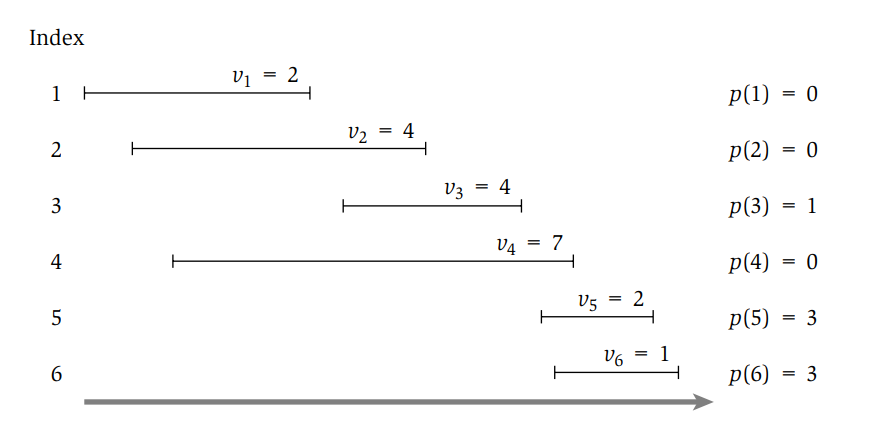
\includegraphics[width=12cm, keepaspectratio]{capitoli/imgs/weighted_problem.png}
    \caption{Istanza di un problema.}
\end{figure}

\section{Goal \normalfont{\emoji{soccer-ball}}}

L'obiettivo del nostro problema attuale è quello di trovare un sottoinsieme $S
    \subseteq \{1, \ldots, n\}$ di intervalli mutualmente compatibili che vanno a
massimizzare la somma dei pesi degli intervalli selezionati $\sum_{i \in S}
    v_i$.

\section{Funzionamento}

Come prima cosa definiamo il metodo per calcolare $OPT(j)$. Il problema è
una \textit{scelta binaria} che va a decidere se l'intervallo di indice $j$
verrà incluso nella soluzione oppure no basandosi sul valore ritornato dalla
seguente formula:

\begin{equation}
    \label{eqn:weight-opt}
    OPT(j) = max(v_j + OPT(p(j)), \ \ OPT(j-1))
\end{equation}
\ \\
Questo può essere anche visto come una disequazione:

\begin{equation}
    \label{eqn:weight-opt-dis}
    v_j + OPT(p(j)) \geq OPT(j-1)
\end{equation}
\ \\
che se vera, includerà $j$ nella soluzione ottimale.

\pagebreak

Scrivendo tutto sotto forma di algoritmo ricorsivo avremmo che:

\begin{lstlisting}[language=Javascript]
    function Compute-Opt(j){
        if (j == 0)
            return 0
        else
            return max(vj+Compute-Opt(p(j)), Compute-Opt(j − 1))
    }
\end{lstlisting}

Costruendo l'albero della ricorsione dell'algoritmo si nota che la complessità
temporale è esponenziale \emoji{astonished} !

\begin{figure}[H]
    \centering
    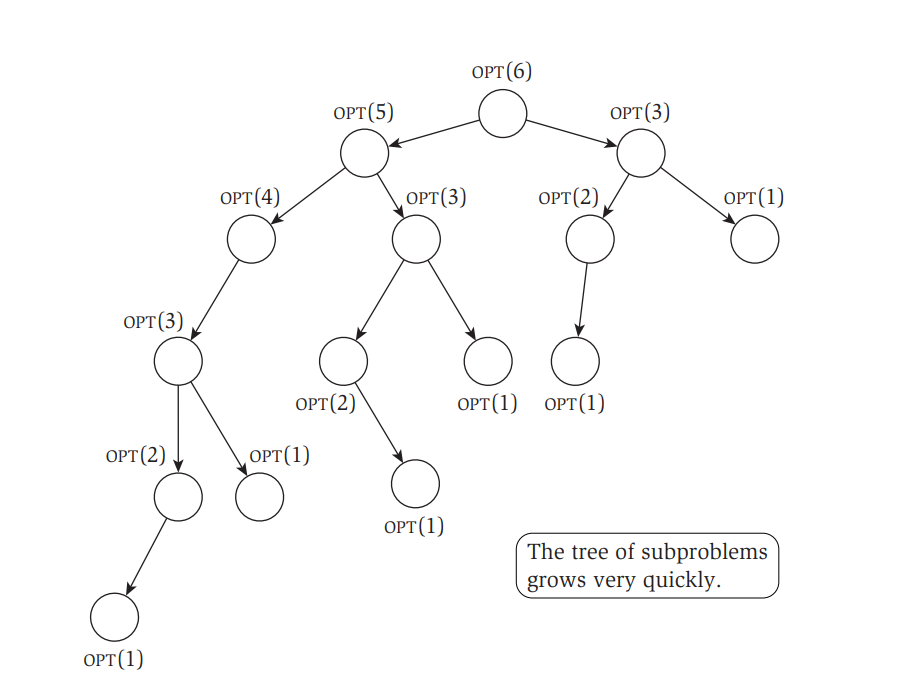
\includegraphics[width=12cm, keepaspectratio]{capitoli/imgs/opt_albero.png}
    \caption{Sviluppo dell'albero di ricorsione per la risoluzione di un problema.}
\end{figure}

\pagebreak

Una soluzione è quella di utilizzare la tecnica della \textbf{Memoization} che evita
di ricalcolare $OPT$ per gli indici già calcolati precedentemente, rendendo così
il costo temporale uguale ad $O(n)$ \emoji{man-in-motorized-wheelchair}.

\begin{lstlisting}[language=Javascript]
function M-Compute-Opt(j){
    if (j == 0)
        return 0
    else if (M[j] is not empty)
        return M[j]
    else
        let M[j] = max(vj+M-Compute-Opt(p(j)), M-Compute-Opt(j-1))
        return M[j]
}
\end{lstlisting}

Oltre al valore della soluzione ottimale probabilmente vorremmo sapere anche
quali sono gli intervalli che la compongono, e intuitivamente verrebbe da creare
un array aggiuntivo in cui verranno aggiunti gli indici degli intervalli
ottenuti con \verb|M-Compute-Opt|. Tuttavia questo aggiungerebbe una complessità
temporale di $O(n)$ peggiorando notevolmente le prestazioni. Un'alternativa è
quella di recuperare le soluzioni dai valori salvati nell'array \verb|M| dopo che la
soluzione ottimale è stata calcolata. Per farlo possiamo sfruttare la formula
vista in precedenza $v_j + OPT(p(j)) \geq OPT(j-1)$, che ci permette di
rintracciare gli intervalli della soluzione ottima.

\begin{lstlisting}[language=Javascript]
    function Find-Solution(j) {
        if (j == 0)
            Output nothing
        else if (vj + M[p(j)] >= M[j-1])
            Output j together with the result 
            of Find-Solution(p(j))
        else
            Output the result of Find-Solution(j-1)
    }
\end{lstlisting}
% \chapter{Least Squares Problem: Multi-way Choice \normalfont{\emoji{motorway}}}

Nel capitolo precedente l'algoritmo richiedeva una ricorsione basata su scelte
binarie, in questo capitolo invece introdurremo un algoritmo che richiede ad
ogni step un numero di scelte polinomiali (\textit{multi-way choice}). Vedremo
come la programmazione dinamica si presta molto bene a risolvere questi
problemi.

\section{Linear Least Square}

\subsection{Il Problema}

La formulazione del problema è la seguente:

\paragraph*{} dato un insieme $P$ composto di $n$ punti sul piano denotati con\\
$(x_1, y_1), (x_2, y_2), \ldots, (x_n, y_n)$; e supponiamo che $x_1 < x_2 <
    \ldots < x_n$ (sono strettamente crescenti). Data una linea $L$ definita
dall'equazione $y = ax + b$, definiamo l'\textit{errore} di $L$ in funzione
di $P$ come la somma delle distanze al quadrato della linea rispetto ai
punti in $P$. Formalmente:
\[
    Error(L, P) = \sum_{i=1}^{n} (y_i - ax_i - b)^2
\]

\begin{figure}[H]
    \centering
    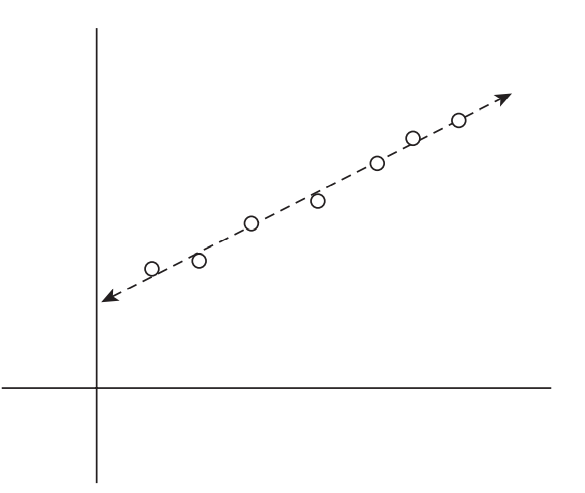
\includegraphics[width=6cm, keepaspectratio]{capitoli/imgs/linear_least.png}
    \caption{Esempio di una tipica istanza e soluzione del problema
        \textit{Linear Least}}
\end{figure}

\subsection{\goal}

È intuibile che il goal dell'algoritmo è quello di cercare la linea con errore
minimo, che può essere facilmente trovata utilizzando l'analisi matematica.
La linea di errore minimo è $y = ax + b$ dove:

\[
    a = \frac{n \sum_{i} x_i y_i - (\sum_{i} x_i) (\sum_{i} y_i)}{n \sum_{i} x_i^2 - (\sum_{i} x_i)^2} \ \ \  \ \ b = \frac{\sum_{i} y_i - a \sum_{i} x_i}{n}
\]

\section{Segmented Least Square}

Le formule appena citate sono utilizzabili solo se i punti di $P$ hanno un
andamento che è abbastanza lineare ma falliscono in altre circostanze.

\begin{figure}[H]
    \centering
    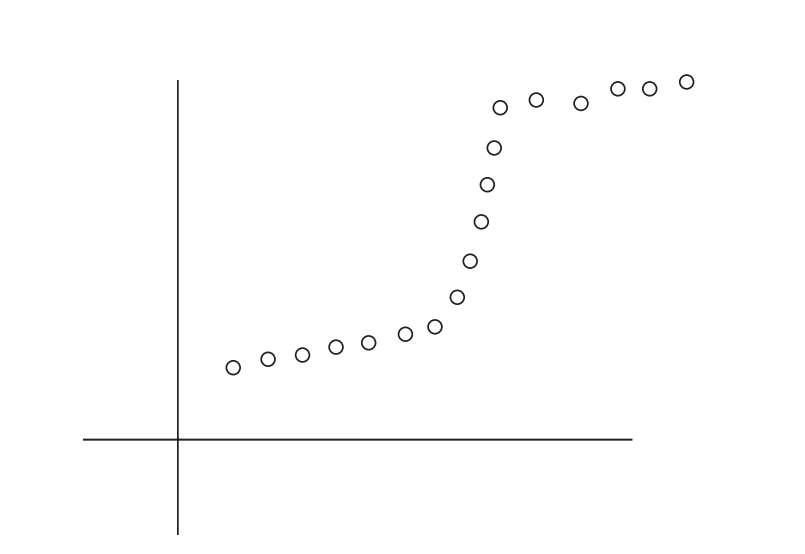
\includegraphics[width=8cm, keepaspectratio]{capitoli/imgs/segmente_linear_least.png}
    \caption{Esempio di funzione non risolvibile con Linear Least Square}
\end{figure}

Come è evidente (\textit{lapalissiano \normalfont{\emoji{gem}}}) dalla figura
non è possibile trovare una linea che approssimi in maniera soddisfacente i
punti, dunque per risolvere il problema possiamo pensare di rilassare la
condizione che sia solo una la linea. Questo però implica dover riformulare il
goal che altrimenti risulterebbe banale (si fanno $n$ linee che passano per ogni
punto).

\subsection{Costi}

La parte che computa gli errori ha costo in tempo $O(n^3)$ (si può portare a
$O(n^2)$).
La parte che trova il valore ottimo ha costo $O(n^2)$.\\

In spazio l'algoritmo ha costo $O(n^2)$ ma può essere ridotto a $O(n)$

\subsection{\goal}

Formalmente, il problema è espresso come segue:

\paragraph*{} come prima abbiamo un set di punti $P = \{(x_1, y_1), (x_2, y_2),
    \ldots, (x_n, y_n)\}$ strettamente crescenti. Denoteremo l'insieme dei punti
$(x_i, y_i)$ con $p_i$. Vogliamo partizionare $P$ in un qualche numero di
segmenti, ogni numero di segmenti è un sottoinsieme di $P$ che rappresenta un
\textit{set} contiguo delle coordinate $x$ con la forma $\{p_i, p_{i+1}, \ldots,
    p_{j-1}, p_j\}$ per degli indici $i \leq j$. Dopodiché, per ogni segmento $S$
calcoliamo la linea che minimizza l'errore rispetto ai punti in $S$ secondo
quanto espresso dalle formule enunciate prima.\\

Definiamo infine una penalità per una data partizione come la somma dei seguenti
termini:

\begin{itemize}
    \item Numero di segmenti in cui viene partizionato $P$ moltiplicato per un
          valore $C > 0$ (più è grande e più penalizza tante partizioni)
    \item Per ogni segmento l'errore della linea ottima attraverso quel
          segmento.
\end{itemize}


Il goal del Segmented Least Square Problem è quindi quello di trovare la
partizione di \textbf{penalità minima}.

\subsection{Funzionamento}

Per come è fatta la programmazione dinamica noi vogliamo suddividere il problema
in sotto-problemi e per farlo partiamo dall'osservazione che l'ultimo punto
appartiene ad una partizione ottima che parte da un valore $p_i$ fino a $p_n$ e
che possiamo togliere questi punti dal totale per ottenete un sotto-problema più
piccolo. Supponiamo che la soluzione ottima sia denotata da \verb|OPT(j)|, per i
punti che vanno da $p_1$ a $p_j$, allora avremo che la soluzione ottima al
problema dato l'ultimo segmento che va da $p_i$ a $p_n$, sarà dalla seguente
formula:

\[
    OPT(n) = e_{i,n} + C + OPT(i - 1)
\]

Questa formula è data dalla soluzione ottima dell'ultima partizione ($e_{i,n} + C$)
a cui viene aggiunta la soluzione ottima di tutte le partizioni precedenti
($OPT(i -1)$). Per i sotto-problemi possiamo scrivere la soluzione al problema
in forma ricorsiva utilizzando la formula appena espressa che prenderà la forma:

\[
    OPT(j) = \min_{1 \leq i \leq j}(e_{i,j} + C + OPT(i - 1))
\]

Possiamo ora dare una versione di questo algoritmo in pseudocodice:

\begin{lstlisting}[language=Javascript]
    function Segmented-Least-Squares(n) {
        M[0 ... n]
        M[0] = 0

        // compute the errors
        for (j in 1 ... n) {
            for (i in 1 ... j) {
                compute eij for the segment pi, ..., pj
            }
        }

        // find optimal value
        for (j in 1 ... n) {
            M[j] = min_i(eij + C + M[i - 1]) // OPT(J)
        }

        return M[n]
    }
\end{lstlisting}

Dopo aver trovato la soluzione ottima, possiamo sfruttare la memoization per
ricavarci i segmenti in tempi brevi.

\begin{lstlisting}[language=Javascript]
    function Find-Segments(j) {
        if (j == 0) print('')

        else {
            Find an i that minimizes ei,j + C + M[i − 1]
            Output the segment {pi,..., pj} and the result of Find-Segments(i − 1)
        }
    }
\end{lstlisting}

L'algoritmo ha costo $O(n^3)$ in tempo e $O(n^2)$ in spazio.
Questo tempo può essere ridotto applicando la memoization alle formule per il calcolo
dell'errore viste in precedenza portandolo a $O(n^2)$ per il tempo e $O(n)$ per lo spazio.
% \chapter{Subset Sum \& Knapsack Problem \normalfont{\emoji{money-bag}}}

\section{Il Problema}

Il problema delle Subset Sum è formalmente definito come segue:\\

\- abbiamo $n$ oggetti $\{1, \ldots, n\}$, a ognuno viene assegnato un
peso non negativo $w_i$ (per $i = 1, \ldots, n$) e ci viene dato anche un
limite $W$. L'obbiettivo è quello di selezionare un sottoinsieme $S$ degli
oggetti tale che $\sum_{i \in S}w_i \leq W$ e che questa sommatoria abbia valore
più grande possibile.\\

Questo problema è un caso specifico di un problema più generale conosciuto come
il Knapsack Problem, l'unica differenza sta nel valore da massimizzare che per il
Knapsack è un valore $v_i$ e non più il peso.

Si potrebbe pensare di risolvere questi problemi con un algoritmo greedy ma
purtroppo non ne esiste uno in grado di trovare efficientemente la soluzione ottima.
Potremmo pensare di ordinare gli oggetti in base al peso in ordine crescente o
decrescente e prenderli, tuttavia questo approccio fallisce per determinati casi
(come per l'insieme $\{W/2+1, W/2, W/2\}$ ordinato in senso decrescente) e l'unica
opzione sarà quella di provare con la programmazione dinamica \emoji{person-in-manual-wheelchair}.
\newpage

\section{\goal}

Possiamo riassumere il goal di questi problemi come segue:\\

\- Abbiamo $n$ oggetti $\{1, \ldots, n\}$, a ognuno viene assegnato un
peso non negativo $w_i$ (per $i = 1, \ldots, n$) e ci viene dato anche un
limite $W$. L'obbiettivo è quello di selezionare un sottoinsieme $S$ degli oggetti
tale che $\sum_{i \in S}w_i \leq W$ e che questa sommatoria abbia valore più
grande possibile.

\section{Costi}

\begin{center}
    \begin{tabular}{|c|c|}
        \centering
        \textbf{Funzione}    & \textbf{Costo (tempo)} \\
        \verb|Subset-Sum|    & $O(nW)$                \\
        \verb|Find-Solution| & $O(n)$                 \\
    \end{tabular}
\end{center}

\section{Funzionamento}

Come per tutti gli algoritmi dinamici dobbiamo cercare dei sotto-problemi e
possiamo utilizzare la stessa intuizione avuto per il problema dello scheduling
(scelta binaria). Facendo tutti i calcoli di dovere otteniamo la seguente
ricorsione:

\begin{center}
    se $w < w_i$ allora $OPT(i, w) = OPT(i-1,w)$ altrimenti\\
    $OPT(i, w) = max(OPT(i-1, w), w_i + OPT(i-1, w-w_i))$
\end{center}

Nella prima parte analizziamo il caso in cui l'elemento che vogliamo aggiungere va
a superare il peso massimo residuo $w$, dunque viene scartato. Nella seconda parte
andiamo ad analizzare se l'aggiunta o meno del nuovo oggetto va a migliorare
la soluzione di $OPT$ che è definita come:\\

\[
    OPT(i, w) = \max_{S} \sum_{j \in S} w_j
\]
\newpage

Possiamo formalizzare il tutto con il seguente pseudo-codice:

\begin{lstlisting}[language=JavaScript]
    function Subset-Sum(n, W) {
        let M[0 . . . n,0... W]

        //initialize the memoization vector
        for(w in 0 ... W) {
            M[0, W] = 0
        }

        //solve subproblems
        for(i in 1 ... n) {
            for(w in 0 ... W) {
                Use the recurrence to compute M[i, w]
            }
        }

        return M[n, W]
    }
\end{lstlisting}

La particolarità di questo algoritmo è che avremmo 2 insiemi di sotto-problemi
diversi che devono essere risolti per ottenere la soluzione ottima. Questo fatto
si riflette in come viene popolato l'array di memoization dei valori di $OPT$
che verranno salvati in un array bidimensionale.

\begin{figure}[H]
    \centering
    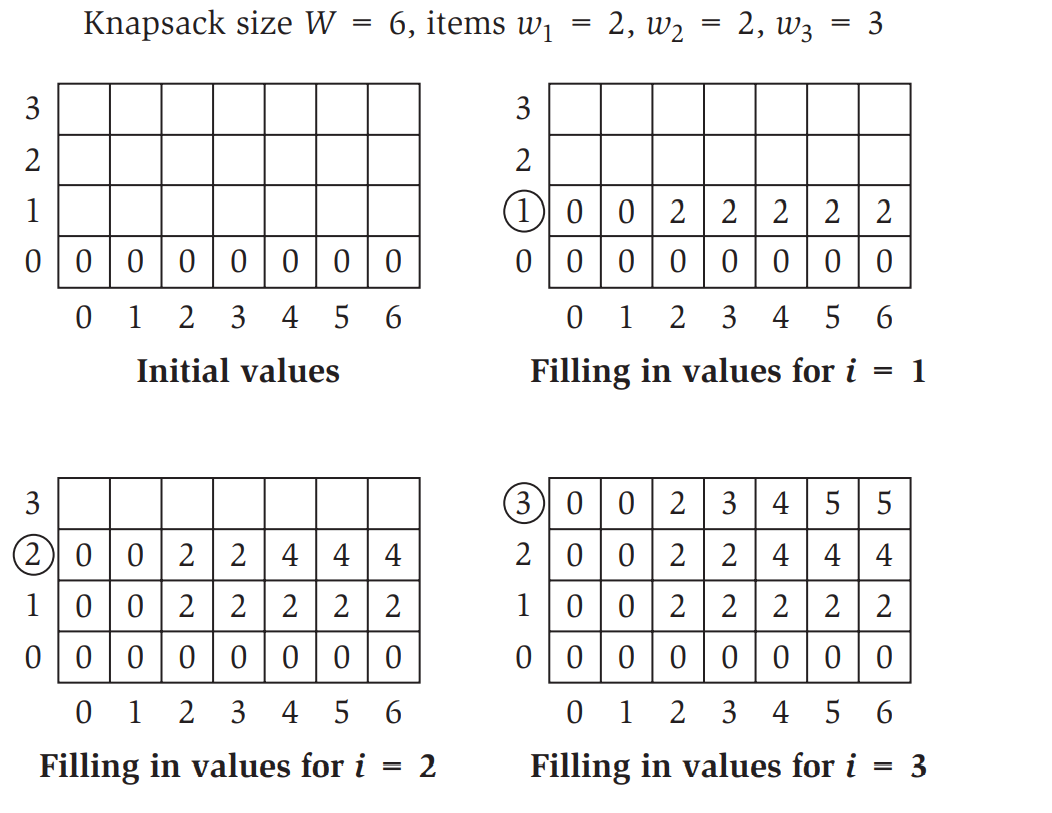
\includegraphics[width=10cm, keepaspectratio]{capitoli/imgs/knapsac_table.png}
    \caption{Esempio di come viene popolato l'array $M$ per il problema del Knapsack.}
\end{figure}

\textit{Il costo in tempo di questa implementazione è di $O(nW)$.}\\

A causa di questo costo, l'algoritmo fa parte della famiglia degli
algoritmi \textit{pseudo polinomiali}, ovvero algoritmi il cui costi dipende da
una variabile di input che se piccola, lo mantiene basso e se grande lo fa
esplodere.\\

\textit{Per recuperare gli oggetti dall'array di Memoization la complessità in tempo è di
    $O(n)$.}\\

Questa implementazione funziona anche per il problema più generale del Knapsack,
ci basterà solo cambiare la parte di ricorsione scrivendola come segue:

\begin{center}
    se $w < w_i$ allora $OPT(i, w) = OPT(i-1,w)$ altrimenti
    $OPT(i, w) = max(OPT(i-1, w), v_i + OPT(i-1, w-w_i))$
\end{center}

La complessità temporale è sempre $O(nW)$.
% \section{RNA Secondary Structure \normalfont{\emoji{dna}}}

La ricerca della struttura secondaria dell'RNA è un problema a 2 variabili
risolvibile tramite il paradigma della programmazione dinamica. Come sappiamo il
DNA è composto da due filamenti, mentre l'RNA è composto da un filamento
singolo. Questo comporta che spesso le basi di un singolo filamento di RNA si
accoppino tra di loro. L'insieme della basi può essere visto come l'alfabeto
$\{A, C, U, G\}$ e l'RNA è una sequenza di simboli presi da questo alfabeto. Il
processo di accoppiamento delle basi è dettato dalla regola di \textit{Watson-Crick} e
segue il seguente schema:

\[
    A - U \ \ \ \textrm{ e } \ \ \ C - G \ \ \ \textrm{ (l'ordine non conta)}
\]

\begin{figure}[H]
    \centering
    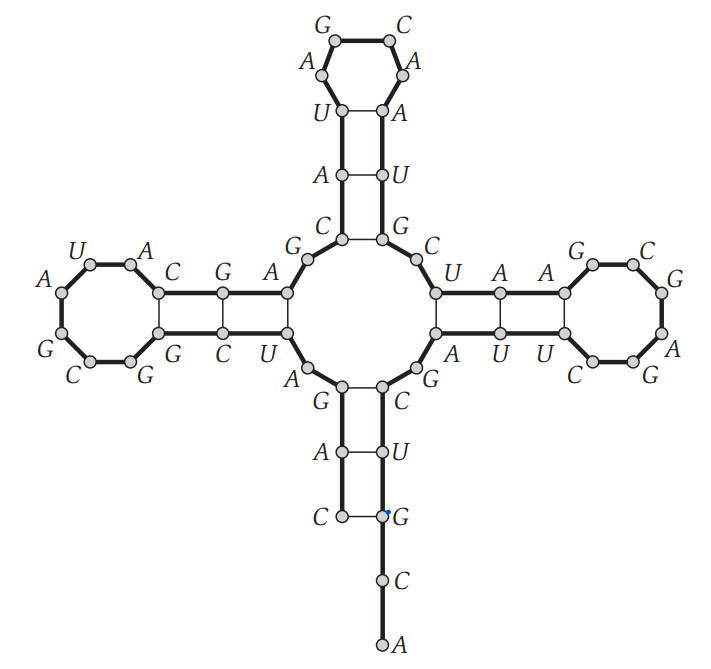
\includegraphics[width=8cm, keepaspectratio]{capitoli/dynamic_programming/imgs/rna_esempio1.png}
    \caption{Esempio di una struttura secondari di RNA} %%TODO: ricontrollare !!
\end{figure}

\subsection{Il Problema}

In questo problema si vuole trovare la struttura secondaria dell'RNA che abbia
energia libera maggiore (il maggior numero di coppie di basi possibili). Per
farlo dobbiamo tenere in considerazione alcune condizioni che devono essere
soddisfatte per permettere di approssimare al meglio il modello biologico
dell'RNA.\\

Formalmente la struttura secondaria di $B$ è un insieme di coppie $S =
    \{(i,j)\}$ dove $i,j \in \{1,2,\ldots,n\}$, che soddisfa le seguenti
condizioni:

\begin{enumerate}
    \item \textbf{No Sharp Turns}: la fine di ogni coppia è separata da almeno 4
          basi, quindi se $(i,j) \in S$ allora $i < j - 4$
    \item Gli elementi di una qualsiasi coppia $S$ consistono di $\{A, U\}$ o
          $\{C, G\}$ (in qualsiasi ordine).
    \item $S$ è un \textit{matching}: nessuna base compare in più di una coppia.
    \item \textbf{Non Crossing Condition}: se $(i, j)$ e $(k,l)$ sono due coppie
          in $S$ allora \textbf{non} può avvenire che $i < k < j < l$.
\end{enumerate}

\begin{figure}[H]
    \centering
    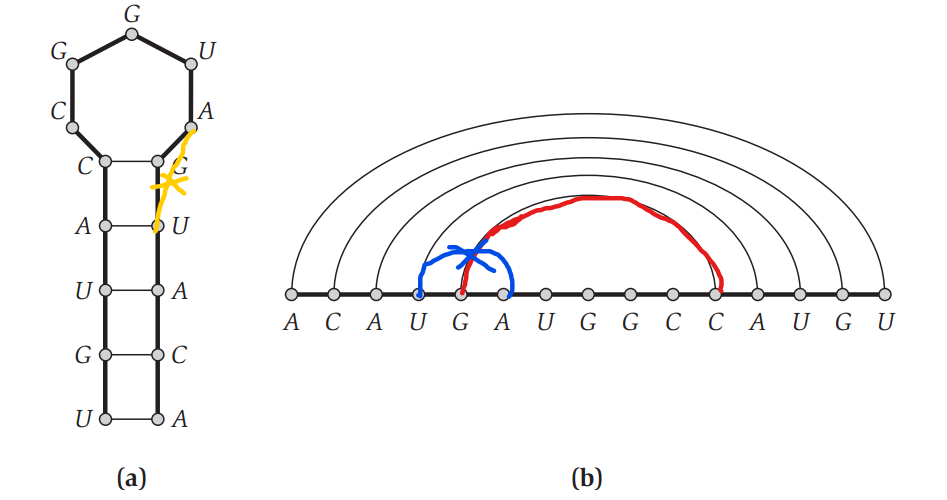
\includegraphics[width=10cm, keepaspectratio]{capitoli/dynamic_programming/imgs/rna_esempio2.png}
    \caption{La figura \textit{(a)} rappresenta un esempio di \textit{Sharp
            Turn}, mentre la figura \textit{(b)} mostra una
        \textit{Crossing Condition} dove il filo blu non dovrebbe esistere.}
\end{figure}

\subsection{\goal}

Il goal di questo problema è di massimizzare la quantità di coppie che si possono
formare all'interno della struttura secondaria di una data sequenza di RNA.

\subsection{Costi}

L'algoritmo complessivo ha costo $O(n^3)$.

\subsection{Funzionamento}

\paragraph{First Attempt.}
Come primo tentativo potremmo basarci sul seguente sotto-problema: affermiamo che
$OPT(j)$ è il massimo numero di coppie di basi sulla struttura secondaria $b_1
    b_2 \ldots b_j$, per la Non Sharp Turn Condition sappiamo che $OPT(j) = 0$ per
$j \leq 5$ e sappiamo anche che $OPT(n)$ è la soluzione che vogliamo trovare. Il
problema ora sta nell'esprimere $OPT(j)$ ricorsivamente. Possiamo parzialmente
farlo sfruttando le seguenti scelte:

\begin{itemize}
    \item $j$ non appartiene ad una coppia
    \item $j$ si accoppia con $t$ per qualche $t \leq
              j - 4$
\end{itemize}

Per il primo caso basta cercare la soluzione per $OPT(j - 1)$, nel secondo caso
invece se teniamo conto della Non Crossing Condition, possiamo isolare due nuovi
sotto-problemi: uno sulle basi $b_1 b_2 \ldots b_{t-1}$ e l'altro sulle basi
$b_{t+1} \ldots b_{j-1}$. Il primo si risolve con $OPT(t-1)$ ma il secondo, dato
che non inizia con indice $1$, non è nella lista dei nostri sotto-problemi. A
causa di ciò risulta necessario aggiungere una variabile.

\begin{figure}[H]
    \centering
    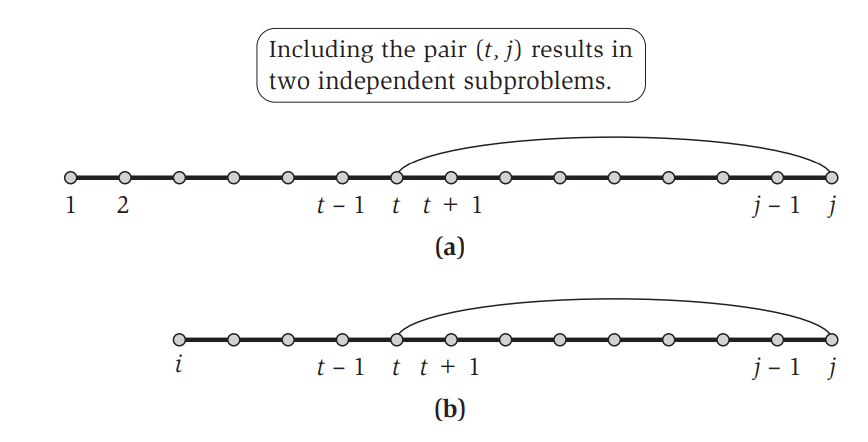
\includegraphics[width=10cm, keepaspectratio]{capitoli/dynamic_programming/imgs/rna_funzionamento.png}
    \caption{Esempio di
        utilizzo di una sola variabile \textit{(a)} o con due \textit{(b)}.}
\end{figure}

\paragraph{Dynamic Programming over Intervals}
Basandoci sui ragionamenti precedenti, possiamo scrivere una ricorsione di
successo: sia $OPT(i,j)$ il numero massimo di coppie di basi nella struttura
secondaria $b_i b_{i+1} \ldots b_j$, grazie alla non sharp turn Condition
possiamo inizializzare gli elementi con $i \geq j -4$ a $0$. Ora avremmo sempre
le stesse condizioni elencate sopra:

\begin{itemize}
    \item $j$ non appartiene ad una coppia
    \item $j$ si accoppia con $t$ per qualche $t \leq j - 4$
\end{itemize}

Nel primo caso avremmo che $OPT(i,j) = OPT(i, j-1)$, nel secondo caso possiamo
ricorrere su due sotto-problemi $OPT(i, t-1)$ e $OPT(t+1, j-1)$ affinché venga
rispettata la non crossing condition. Possiamo esprimere formalmente la
ricorsione come segue:

\begin{center}
    \[
        OPT(i, j) = \max(OPT(i, j-1), \max_t(1+OPT(i, t-1)+OPT(t+1, j-1))),
    \]
    dove il massimo è calcolato su $t$ tale che $b_t$ e $b_j$ siano una coppia di
    basi consentita
\end{center}

\begin{figure}[H]
    \centering
    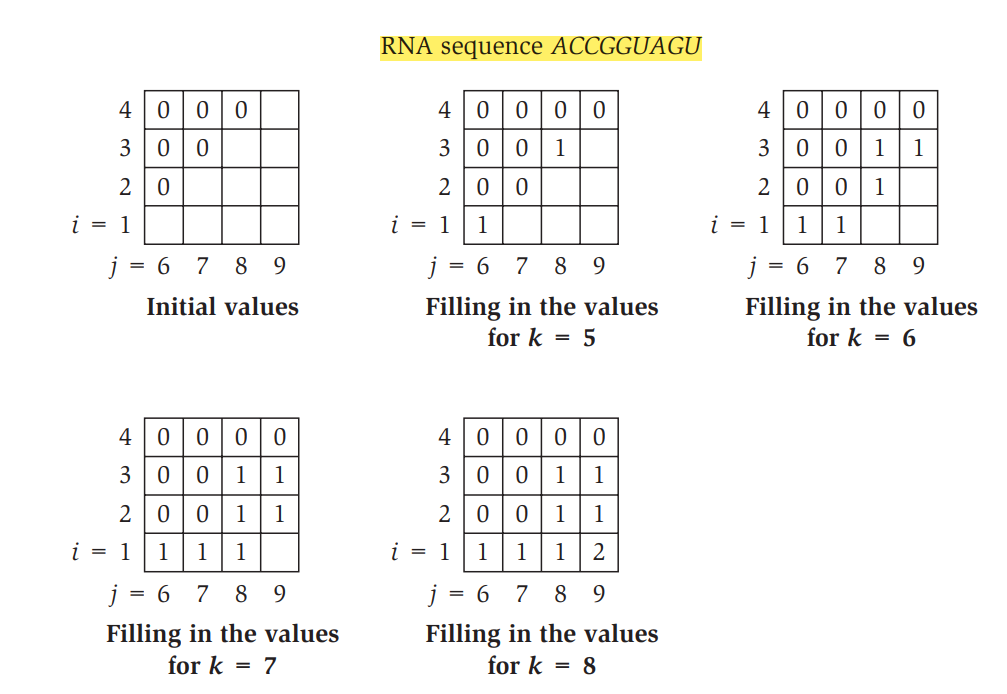
\includegraphics[width=\textwidth, keepaspectratio]{capitoli/dynamic_programming/imgs/rna_calcolo.png}
    \caption{Iterazioni dell'algoritmo su un campione del problema in questione $ACCGGUAGU$}
\end{figure}
\newpage

Possiamo infine formalizzare il tutto con il seguente pseudo-codice:

\begin{lstlisting}[language=JavaScript]
 Initialize OPT(i, j) = 0 whenever i ≥ j - 4

 for (k in 5 ... n - 1) {
     for (i in 1 ... n - k) {
         j = i + k
         Compute OPT(i, j) using the previous recurrence
     }
 }

 return OPT(1, n)
\end{lstlisting}

Ci sono $O(n^2)$ sotto-problemi da risolvere e ognuno richiede tempo $O(n)$,
quindi il running time complessivo è di $O(n^3)$.

% \section{Sequence Alignment}

Il problema del Sequence Alignment consiste nel riuscire a comparare delle
stringhe, come per esempio quando si effettua un typo in un motore di ricerca e
quello ci fornisce l'alternativa corretta. Una prima idea potrebbe essere quella
di \textbf{allineare} le due parole lettera per lettera, riempendo gli eventuali
spazi bianchi, e vedendo di quanto le due differiscono. Tuttavia ci sono varie
possibilità con cui due parole di lunghezza diversa possono essere confrontate,
quindi è necessario fornire una definizione di \textbf{similarità}.

\subsection{Il Problema}

Come prima definizione di similarità possiamo dire che minore sarà il numero di
caratteri che non corrispondono, maggiore sarà la similarità tra le parole.
Questa problematica è anche un tema centrale della biologia molecolare, e
proprio grazie ad un biologo abbiamo una definizione rigorosa e soddisfacente di
similarità. Prima di dare una definizione similarità dovremo però darne una di
\textbf{allineamento}: Supponiamo di avere due stringhe $X$ e $Y$, che consistono rispettivamente
della sequenza di simboli $x_1 x_2 \ldots x_m$ e $y_1 y_2 \ldots y_n$, e
consideriamo gli insiemi $\{1,2,\ldots ,m\}$ e $\{1,2,\ldots ,n\}$ che
rappresentano le varie posizioni nelle stringhe $X$ e $Y$, ora si considera un
\textbf{Matching} di queste due parole (un matching è stato definito nella parte
precedente e si tratta di un insieme di coppie ordinate con la proprietà che
ogni oggetto si trova al più in una sola coppia).  Diciamo ora che un matching
$M$ di questi due insiemi è un allineamento se gli elementi di varie coppie non
si incrociano: se $(i,j),(i^{\prime},j^{\prime}) \in M$  e $i < i^{\prime}$,
allora $j < j^{\prime}$.\\

Ora la nostra definizione di similarità si baserà sul trovare il miglior
allineamento, seguendo i seguenti criteri:

\begin{itemize}
    \item C'è un parametro $\delta>0$ che
          definisce la \textbf{gap penalty}, ovvero ogni volta che un simbolo di una parola
          non corrisponde ad un simbolo dell'altra.
    \item Per ogni coppia di lettere $p,q$ del
          nostro alfabeto, se c'è un accoppiamento errato si paga il corrispondente
          \textbf{mismatch cost} $a_(p,q)$.
    \item Il costo di $M$ è la somma del suo gap e mismatch
          cost, e l'obiettivo sarà quello di minimizzarlo.
\end{itemize}

\subsection{Creazione dell'algoritmo}

Ora affronteremo il problema di calcolarci questo costo minimo, e l'allineamento
ottimale che lo fornisce date le coppie $X$ e $Y$. Come al solito proveremo con
un approccio di programmazione dinamica, e per realizzare l'algoritmo
individuiamo come per altri algoritmi già visti una scelta binaria. Dato
l'allineamento ottimale $M$ allora:

\begin{itemize}
    \item $(m,n) \in M$ (quindi gli ultimi due
          simboli delle 2 stringhe sono in un matching)
    \item $(m,n) \notin M$ (gli ultimi
          simboli delle due stringhe non sono in un matching)
\end{itemize}

Tuttavia questa semplice distinzione non è sufficiente, quindi supponiamo di
aggiungere anche il seguente fatto elementare:\\

\- Sia $M$ un qualsiasi allineamento di $X$ e $Y$. se $(m,n) \notin M$, allora o
l' $m-esima$ posizione di $X$ o l' $n-esima$ posizione di $Y$ non è in un
matching di $M$.\\

Dire questo equivale a riscrivere le due condizioni sopra come tre, dunque in un
allineamento ottimo $M$ almeno una deve essere vera:

\begin{itemize}
    \item $(m,n) \in M$
    \item l'$m-esima$ posizione di $X$ non è nel matching
    \item l' $n-esima$ posizione di $Y$ non è nel matching
\end{itemize}

Ora definiamo la funzione di costo minimo $OPT(i,j)$ come costo dell'alignmet
tra $x_1 x_2 \ldots x_i$ e $y_1 y_2 \ldots y_j$. In base alle condizioni
espresse in precedenza la funzione $OPT(m,n)$ assumerà il costo relativo più
$OPT(m-1,n-1)$, in particolare (i tre casi citati sopra):

\begin{itemize}
    \item condizione 1, si
          paga un matching cost per le lettere $m,n$
    \item condizione 2 e 3, si paga un gap
          cost $\delta$ per $m$(condizione 2) o $n$(condizione 3)
\end{itemize}

Utilizzando dunque gli stessi argomenti per per i sotto problemi per
l'allineamento di costo minimo tra $X$ e $Y$ otteniamo la definizione generale
di $OPT(i,j)$:\\

L'allineamento di costo minimo soddisfa la seguente ricorsione per $i \geq 1$
e $j \geq 1$:
\[
    OPT(i,j) = min[a_{(x_i y_j)} + OPT(i-1, j-1),
            \delta + OPT(i-1, j), \delta + OPT(i, j-1)]
\]

Dunque così abbiamo ottenuto la nostra funzione di ricorsione e possiamo
procedere alla scrittura dello pseudo codice.

\begin{lstlisting}[language=JavaScript]
    function alignment(X,Y) { var A = Matrix(m, n)

        Initialize A[i, 0]= iδ for each i 
        Initialize A[0, j]= jδ for each j

        for (j in 1...n) { 
            for (i in 1...m) { 
                Use the recurrence (6.16) to compute A[i, j] 
            }
        }

        return A[m, n]
    }
\end{lstlisting}

Il running time è di $O(mn)$

\subsection{Sequence Alignment in Spazio Lineare}

Come abbiamo appena visto l'algoritmo ha sia costo spaziale che temporale uguale
a $O(mn)$ e se come input consideriamo le parole della lingua inglese non
risulta essere un grande problema, ma se consideriamo genomi con 10 miliardi di
caratteri potrebbe risultare difficile poter lavorare con array di 10 GB \emoji{astonished}.
Questo problema può essere risolto utilizzando un approccio \textit{divide et impera}
che va a rendere lineare il costo dello spazio ( $O(n + m)$ ).

\subsubsection{Funzionamento}

Come prima cosa definiamo un algoritmo Space Efficient Alignment che ci permette
di trovare la soluzione ottima utilizzando il minor spazio possibile. Per farlo
notiamo che la funzione $OPT$ dipende solamente da una colonna precedente di
quella che si sta analizzando, dunque basterà caricarsi in memoria una matrice
$mx2$ riducendo così il costo spaziale ad $m$. Tuttavia utilizzando questo
metodo non e possibile ricurvare l'alignment effettivo perché non ci bastano le
informazioni.\\

Lo pseudo-codice dell'algoritmo appena definito è il seguente:

\begin{lstlisting}[language=JavaScript]
    function Space-Efficient-Alignment(X,Y) {
        var B = Matrix(m, 2)

        // (just as in column 0 of A)
        Initialize B[i, 0]= iδ for each i 

        for (j in 1...n) {
            B[0, 1]= jδ (since this corresponds to entry A[0, j])

            for (i in 1...m) {
                B[i, 1]= min[
                    αxiyj + B[i − 1, 0],
                    δ + B[i − 1, 1], 
                    δ + B[i, 0]
                ]
            }

            Move column 1 of B to column 0 to make room 
            for next iteration:
            Update B[i, 0] = B[i, 1] for each i
        }
    }
\end{lstlisting}

Possiamo quindi utilizzare un approccio \textit{divide et impera} che incorpora 2
tecniche diverse di programmazione dinamica per sfruttare questo approccio
appena definito e riuscire a trovare anche l'alignment in spazio lineare.
Definiamo quindi due funzioni:

\begin{itemize}
    \item $f(i, j)$ : è la funzione definita per l'algoritmo di Sequence
          Alignment di base (analoga a $OPT(i,j)$ )
    \item $g(i, j)$ : è l'analogo al contrario di $f$ ed è definito dalla
          seguente funzione ricorsiva: per $i < m$ e $j < n$ : $g(i,j) =
              min[a_{x+1y+1} + g(i+1, j+1), \delta + g(i, j+1), \delta + g(i+1, j)]$
\end{itemize}

Possiamo notare che la ricorsione $f$ procede a ritroso partendo dal fondo
mentre la ricorsione $g$ procede in avanti partendo dall'inizio. Possiamo
sfruttare questo fatto per provare ad utilizzare lo Space Efficiente Sequence
Alignment Algorithm combinato ad un approccio \textit{divide et impera} e un array di
supporto $P$ per riuscire a calcolare il Sequence Alignment in spazio lineare,
aumentando solo di una costatane la complessità temporale.\\

Possiamo riassumere il tutto con il seguente pseudo-codice:

\begin{lstlisting}[language=JavaScript]
    function Divide-and-Conquer-Alignment(X,Y) {
        var m = length(X)
        var n = length(Y)

        if (m <= 2 or n <= 2) {
            Compute optimal alignment using Alignment(X,Y)
        }

        Space-Efficient-Alignment(X, Y[1 : n/2])
        Backward-Space-Efficient-Alignment(X, Y[n/2 + 1 : n])

        Let q be the index minimizing f(q, n/2) + g(q, n/2)
        Add (q, n/2) to global list P

        Divide-and-Conquer-Alignment(X[1 : q],Y[1 : n/2])
        Divide-and-Conquer-Alignment(X[q + 1 : n],Y[n/2 + 1:n])

        return P
    }
\end{lstlisting}

\begin{figure}[H]
    \centering
    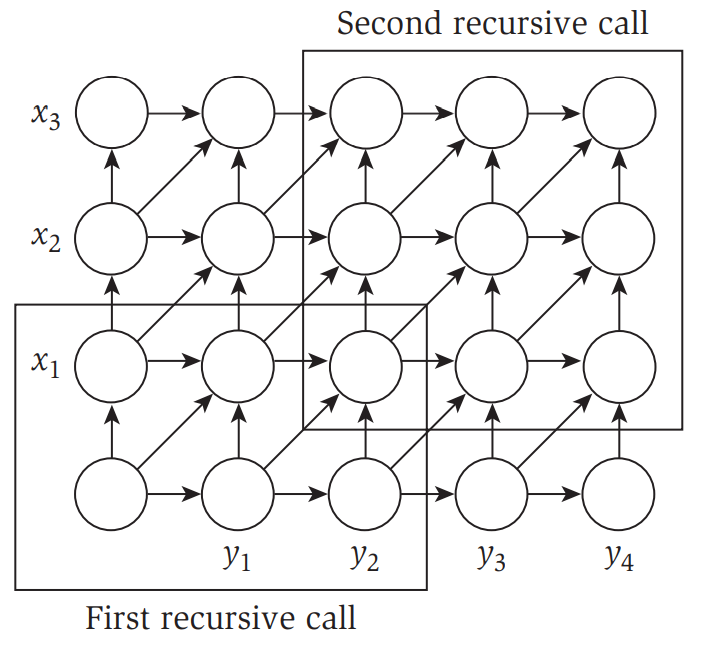
\includegraphics[width=8cm, keepaspectratio]{capitoli/dynamic_programming/imgs/seq_align_recurrence.png}
    \caption{La figura mostra il funzionamento dell'algoritmo appena descritto.}
\end{figure}

\documentclass[a4paper,12 pt]{report}
\usepackage[T1]{fontenc}
\usepackage[utf8]{inputenc}
% \usepackage{amsmath}
\usepackage{lmodern}
\usepackage{listings}
\usepackage{graphicx}
\usepackage{float}
\usepackage{subcaption}
\usepackage{hyperref}
\usepackage{wrapfig}
\usepackage{fancyhdr}
% \usepackage{tcolorbox}

% forza le footnote a stare il più in basso possibile
\usepackage[bottom]{footmisc}
\usepackage{enumitem}

%% STILE LISTINGS

\usepackage{xcolor}

\definecolor{codegreen}{rgb}{0,0.6,0}
\definecolor{codegray}{rgb}{0.5,0.5,0.5}
\definecolor{codepurple}{rgb}{0.58,0,0.82}
\definecolor{backcolour}{rgb}{0.95,0.95,0.92}

\lstdefinestyle{mystyle}{
    backgroundcolor=\color{backcolour},   
    commentstyle=\color{codegreen},
    keywordstyle=\color{magenta},
    numberstyle=\tiny\color{codegray},
    stringstyle=\color{codepurple},
    basicstyle=\ttfamily\footnotesize,
    breakatwhitespace=false,         
    breaklines=true,                 
    captionpos=b,                    
    keepspaces=true,                 
    numbers=left,                    
    numbersep=5pt,                  
    showspaces=false,                
    showstringspaces=false,
    showtabs=false,                  
    tabsize=2
}

\lstset{style=mystyle}

%% SOLIDITY Settings

% Copyright 2017 Sergei Tikhomirov, MIT License
% https://github.com/s-tikhomirov/solidity-latex-highlighting/

%\usepackage{listings, xcolor}

\definecolor{verylightgray}{rgb}{.97,.97,.97}

\lstdefinelanguage{Solidity}{
	keywords=[1]{anonymous, assembly, assert, balance, break, call, callcode, case, catch, class, constant, continue, constructor, contract, debugger, default, delegatecall, delete, do, else, emit, event, experimental, export, external, false, finally, for, function, gas, if, implements, import, in, indexed, instanceof, interface, internal, is, length, library, log0, log1, log2, log3, log4, memory, modifier, new, payable, pragma, private, protected, public, pure, push, require, return, returns, revert, selfdestruct, send, solidity, storage, struct, suicide, super, switch, then, this, throw, transfer, true, try, typeof, using, value, view, while, with, addmod, ecrecover, keccak256, mulmod, ripemd160, sha256, sha3}, % generic keywords including crypto operations
	keywordstyle=[1]\color{blue}\bfseries,
	keywords=[2]{address, bool, byte, bytes, bytes1, bytes2, bytes3, bytes4, bytes5, bytes6, bytes7, bytes8, bytes9, bytes10, bytes11, bytes12, bytes13, bytes14, bytes15, bytes16, bytes17, bytes18, bytes19, bytes20, bytes21, bytes22, bytes23, bytes24, bytes25, bytes26, bytes27, bytes28, bytes29, bytes30, bytes31, bytes32, enum, int, int8, int16, int24, int32, int40, int48, int56, int64, int72, int80, int88, int96, int104, int112, int120, int128, int136, int144, int152, int160, int168, int176, int184, int192, int200, int208, int216, int224, int232, int240, int248, int256, mapping, string, uint, uint8, uint16, uint24, uint32, uint40, uint48, uint56, uint64, uint72, uint80, uint88, uint96, uint104, uint112, uint120, uint128, uint136, uint144, uint152, uint160, uint168, uint176, uint184, uint192, uint200, uint208, uint216, uint224, uint232, uint240, uint248, uint256, var, void, ether, finney, szabo, wei, days, hours, minutes, seconds, weeks, years},	% types; money and time units
	keywordstyle=[2]\color{teal}\bfseries,
	keywords=[3]{block, blockhash, coinbase, difficulty, gaslimit, number, timestamp, msg, data, gas, sender, sig, value, now, tx, gasprice, origin},	% environment variables
	keywordstyle=[3]\color{violet}\bfseries,
	identifierstyle=\color{black},
	sensitive=false,
	comment=[l]{//},
	morecomment=[s]{/*}{*/},
	commentstyle=\color{gray}\ttfamily,
	stringstyle=\color{red}\ttfamily,
	morestring=[b]',
	morestring=[b]"
}

\lstdefinelanguage{JavaScript}{
  keywords={typeof, new, true, false, catch, function, return, null, catch, switch, var, if, in, while, do, else, case, break},
  keywordstyle=\color{blue}\bfseries,
  ndkeywords={class, export, boolean, throw, implements, import, this},
  ndkeywordstyle=\color{darkgray}\bfseries,
  identifierstyle=\color{black},
  sensitive=false,
  comment=[l]{//},
  morecomment=[s]{/*}{*/},
  commentstyle=\color{purple}\ttfamily,
  stringstyle=\color{red}\ttfamily,
  morestring=[b]',
  morestring=[b]"
}
%\lstset{
%	language=Solidity,
%	backgroundcolor=\color{verylightgray},
%	extendedchars=true,
%	basicstyle=\footnotesize\ttfamily,
%	showstringspaces=false,
%	showspaces=false,
%	numbers=left,
%	numberstyle=\footnotesize,
%	numbersep=9pt,
%	tabsize=2,
%	breaklines=true,
%	showtabs=false,
%	captionpos=b
%}

%% -----

% box around text
\newenvironment{boxed}
    {\begin{center}
    \begin{tabular}{|p{\textwidth}|}
    \hline\\
    }
    { 
    \\\\\hline
    \end{tabular} 
    \end{center}
    }

% Resetta la numerazione dei chapter quando
% una nuova part viene creata
\makeatletter
\@addtoreset{chapter}{part}
\makeatother

% Rimuove l'indentazione quando si crea un nuovo paragrafo
\setlength{\parindent}{0pt}

% footer
\pagestyle{fancyplain}
% rimuove la riga nell'header
\fancyhf{} % sets both header and footer to nothing
\renewcommand{\headrulewidth}{0pt}
\fancyfoot[L]{\href{https://github.com/Typing-Monkeys/AppuntiUniversita}{Typing Monkeys}}
\fancyfoot[C]{\emoji{gorilla}}
\fancyfoot[R]{\thepage}

% configurazione emoji
\usepackage{fontspec}
\usepackage{emoji}
\setemojifont{NotoColorEmoji.ttf}[Path=/usr/share/fonts/truetype/noto/]


% Macro
\newcommand{\goal}{Goal \normalfont{\emoji{soccer-ball}}}


\begin{document}
\include{frontmatter/main.tex}

%% TODO: riorganizzare la struttura degli appunti
%%       alla fine dovremmo avere una roba del tipo
%%          - Programmazione Dinamica
%%            - Arg 1
%%            - Arg 2
%%              - subarg 1
%%              - subarg 2
%%          - Flow
%%            - Arg 1
%%              - sub arg 1
%%          - Graph
%%            - Arg 1
%%

\tableofcontents

\include{quote/main.tex}

% \include{capitoli/dynamic_programming/1-introduzione_all_programmazione_dinamica.tex}
% \include{capitoli/dynamic_programming/2-weighted_interval_scheduling.tex}
% \include{capitoli/dynamic_programming/3-least_squares_problem_multiway_choice.tex}
% \include{capitoli/dynamic_programming/4-subset_sum_e_knapsack_problem.tex}
% \include{capitoli/dynamic_programming/5-rna_secondary_structure.tex}
% \include{capitoli/dynamic_programming/6-sequence_alignment.tex}
\include{capitoli/dynamic_programming/main.tex}

\end{document}

\end{document}

%% TODO: riorganizzare la struttura degli appunti
%%       alla fine dovremmo avere una roba del tipo
%%          - Programmazione Dinamica
%%            - Arg 1
%%            - Arg 2
%%              - subarg 1
%%              - subarg 2
%%          - Flow
%%            - Arg 1
%%              - sub arg 1
%%          - Graph
%%            - Arg 1
%%

\tableofcontents

\documentclass[a4paper,12 pt]{report}
\usepackage[T1]{fontenc}
\usepackage[utf8]{inputenc}
% \usepackage{amsmath}
\usepackage{lmodern}
\usepackage{listings}
\usepackage{graphicx}
\usepackage{float}
\usepackage{subcaption}
\usepackage{hyperref}
\usepackage{wrapfig}
\usepackage{fancyhdr}
% \usepackage{tcolorbox}

% forza le footnote a stare il più in basso possibile
\usepackage[bottom]{footmisc}
\usepackage{enumitem}

%% STILE LISTINGS

\usepackage{xcolor}

\definecolor{codegreen}{rgb}{0,0.6,0}
\definecolor{codegray}{rgb}{0.5,0.5,0.5}
\definecolor{codepurple}{rgb}{0.58,0,0.82}
\definecolor{backcolour}{rgb}{0.95,0.95,0.92}

\lstdefinestyle{mystyle}{
    backgroundcolor=\color{backcolour},   
    commentstyle=\color{codegreen},
    keywordstyle=\color{magenta},
    numberstyle=\tiny\color{codegray},
    stringstyle=\color{codepurple},
    basicstyle=\ttfamily\footnotesize,
    breakatwhitespace=false,         
    breaklines=true,                 
    captionpos=b,                    
    keepspaces=true,                 
    numbers=left,                    
    numbersep=5pt,                  
    showspaces=false,                
    showstringspaces=false,
    showtabs=false,                  
    tabsize=2
}

\lstset{style=mystyle}

%% SOLIDITY Settings

% Copyright 2017 Sergei Tikhomirov, MIT License
% https://github.com/s-tikhomirov/solidity-latex-highlighting/

%\usepackage{listings, xcolor}

\definecolor{verylightgray}{rgb}{.97,.97,.97}

\lstdefinelanguage{Solidity}{
	keywords=[1]{anonymous, assembly, assert, balance, break, call, callcode, case, catch, class, constant, continue, constructor, contract, debugger, default, delegatecall, delete, do, else, emit, event, experimental, export, external, false, finally, for, function, gas, if, implements, import, in, indexed, instanceof, interface, internal, is, length, library, log0, log1, log2, log3, log4, memory, modifier, new, payable, pragma, private, protected, public, pure, push, require, return, returns, revert, selfdestruct, send, solidity, storage, struct, suicide, super, switch, then, this, throw, transfer, true, try, typeof, using, value, view, while, with, addmod, ecrecover, keccak256, mulmod, ripemd160, sha256, sha3}, % generic keywords including crypto operations
	keywordstyle=[1]\color{blue}\bfseries,
	keywords=[2]{address, bool, byte, bytes, bytes1, bytes2, bytes3, bytes4, bytes5, bytes6, bytes7, bytes8, bytes9, bytes10, bytes11, bytes12, bytes13, bytes14, bytes15, bytes16, bytes17, bytes18, bytes19, bytes20, bytes21, bytes22, bytes23, bytes24, bytes25, bytes26, bytes27, bytes28, bytes29, bytes30, bytes31, bytes32, enum, int, int8, int16, int24, int32, int40, int48, int56, int64, int72, int80, int88, int96, int104, int112, int120, int128, int136, int144, int152, int160, int168, int176, int184, int192, int200, int208, int216, int224, int232, int240, int248, int256, mapping, string, uint, uint8, uint16, uint24, uint32, uint40, uint48, uint56, uint64, uint72, uint80, uint88, uint96, uint104, uint112, uint120, uint128, uint136, uint144, uint152, uint160, uint168, uint176, uint184, uint192, uint200, uint208, uint216, uint224, uint232, uint240, uint248, uint256, var, void, ether, finney, szabo, wei, days, hours, minutes, seconds, weeks, years},	% types; money and time units
	keywordstyle=[2]\color{teal}\bfseries,
	keywords=[3]{block, blockhash, coinbase, difficulty, gaslimit, number, timestamp, msg, data, gas, sender, sig, value, now, tx, gasprice, origin},	% environment variables
	keywordstyle=[3]\color{violet}\bfseries,
	identifierstyle=\color{black},
	sensitive=false,
	comment=[l]{//},
	morecomment=[s]{/*}{*/},
	commentstyle=\color{gray}\ttfamily,
	stringstyle=\color{red}\ttfamily,
	morestring=[b]',
	morestring=[b]"
}

\lstdefinelanguage{JavaScript}{
  keywords={typeof, new, true, false, catch, function, return, null, catch, switch, var, if, in, while, do, else, case, break},
  keywordstyle=\color{blue}\bfseries,
  ndkeywords={class, export, boolean, throw, implements, import, this},
  ndkeywordstyle=\color{darkgray}\bfseries,
  identifierstyle=\color{black},
  sensitive=false,
  comment=[l]{//},
  morecomment=[s]{/*}{*/},
  commentstyle=\color{purple}\ttfamily,
  stringstyle=\color{red}\ttfamily,
  morestring=[b]',
  morestring=[b]"
}
%\lstset{
%	language=Solidity,
%	backgroundcolor=\color{verylightgray},
%	extendedchars=true,
%	basicstyle=\footnotesize\ttfamily,
%	showstringspaces=false,
%	showspaces=false,
%	numbers=left,
%	numberstyle=\footnotesize,
%	numbersep=9pt,
%	tabsize=2,
%	breaklines=true,
%	showtabs=false,
%	captionpos=b
%}

%% -----

% box around text
\newenvironment{boxed}
    {\begin{center}
    \begin{tabular}{|p{\textwidth}|}
    \hline\\
    }
    { 
    \\\\\hline
    \end{tabular} 
    \end{center}
    }

% Resetta la numerazione dei chapter quando
% una nuova part viene creata
\makeatletter
\@addtoreset{chapter}{part}
\makeatother

% Rimuove l'indentazione quando si crea un nuovo paragrafo
\setlength{\parindent}{0pt}

% footer
\pagestyle{fancyplain}
% rimuove la riga nell'header
\fancyhf{} % sets both header and footer to nothing
\renewcommand{\headrulewidth}{0pt}
\fancyfoot[L]{\href{https://github.com/Typing-Monkeys/AppuntiUniversita}{Typing Monkeys}}
\fancyfoot[C]{\emoji{gorilla}}
\fancyfoot[R]{\thepage}

% configurazione emoji
\usepackage{fontspec}
\usepackage{emoji}
\setemojifont{NotoColorEmoji.ttf}[Path=/usr/share/fonts/truetype/noto/]


% Macro
\newcommand{\goal}{Goal \normalfont{\emoji{soccer-ball}}}


\begin{document}
\documentclass[a4paper,12 pt]{report}
\usepackage[T1]{fontenc}
\usepackage[utf8]{inputenc}
% \usepackage{amsmath}
\usepackage{lmodern}
\usepackage{listings}
\usepackage{graphicx}
\usepackage{float}
\usepackage{subcaption}
\usepackage{hyperref}
\usepackage{wrapfig}
\usepackage{fancyhdr}
% \usepackage{tcolorbox}

% forza le footnote a stare il più in basso possibile
\usepackage[bottom]{footmisc}
\usepackage{enumitem}

%% STILE LISTINGS

\usepackage{xcolor}

\definecolor{codegreen}{rgb}{0,0.6,0}
\definecolor{codegray}{rgb}{0.5,0.5,0.5}
\definecolor{codepurple}{rgb}{0.58,0,0.82}
\definecolor{backcolour}{rgb}{0.95,0.95,0.92}

\lstdefinestyle{mystyle}{
    backgroundcolor=\color{backcolour},   
    commentstyle=\color{codegreen},
    keywordstyle=\color{magenta},
    numberstyle=\tiny\color{codegray},
    stringstyle=\color{codepurple},
    basicstyle=\ttfamily\footnotesize,
    breakatwhitespace=false,         
    breaklines=true,                 
    captionpos=b,                    
    keepspaces=true,                 
    numbers=left,                    
    numbersep=5pt,                  
    showspaces=false,                
    showstringspaces=false,
    showtabs=false,                  
    tabsize=2
}

\lstset{style=mystyle}

%% SOLIDITY Settings

% Copyright 2017 Sergei Tikhomirov, MIT License
% https://github.com/s-tikhomirov/solidity-latex-highlighting/

%\usepackage{listings, xcolor}

\definecolor{verylightgray}{rgb}{.97,.97,.97}

\lstdefinelanguage{Solidity}{
	keywords=[1]{anonymous, assembly, assert, balance, break, call, callcode, case, catch, class, constant, continue, constructor, contract, debugger, default, delegatecall, delete, do, else, emit, event, experimental, export, external, false, finally, for, function, gas, if, implements, import, in, indexed, instanceof, interface, internal, is, length, library, log0, log1, log2, log3, log4, memory, modifier, new, payable, pragma, private, protected, public, pure, push, require, return, returns, revert, selfdestruct, send, solidity, storage, struct, suicide, super, switch, then, this, throw, transfer, true, try, typeof, using, value, view, while, with, addmod, ecrecover, keccak256, mulmod, ripemd160, sha256, sha3}, % generic keywords including crypto operations
	keywordstyle=[1]\color{blue}\bfseries,
	keywords=[2]{address, bool, byte, bytes, bytes1, bytes2, bytes3, bytes4, bytes5, bytes6, bytes7, bytes8, bytes9, bytes10, bytes11, bytes12, bytes13, bytes14, bytes15, bytes16, bytes17, bytes18, bytes19, bytes20, bytes21, bytes22, bytes23, bytes24, bytes25, bytes26, bytes27, bytes28, bytes29, bytes30, bytes31, bytes32, enum, int, int8, int16, int24, int32, int40, int48, int56, int64, int72, int80, int88, int96, int104, int112, int120, int128, int136, int144, int152, int160, int168, int176, int184, int192, int200, int208, int216, int224, int232, int240, int248, int256, mapping, string, uint, uint8, uint16, uint24, uint32, uint40, uint48, uint56, uint64, uint72, uint80, uint88, uint96, uint104, uint112, uint120, uint128, uint136, uint144, uint152, uint160, uint168, uint176, uint184, uint192, uint200, uint208, uint216, uint224, uint232, uint240, uint248, uint256, var, void, ether, finney, szabo, wei, days, hours, minutes, seconds, weeks, years},	% types; money and time units
	keywordstyle=[2]\color{teal}\bfseries,
	keywords=[3]{block, blockhash, coinbase, difficulty, gaslimit, number, timestamp, msg, data, gas, sender, sig, value, now, tx, gasprice, origin},	% environment variables
	keywordstyle=[3]\color{violet}\bfseries,
	identifierstyle=\color{black},
	sensitive=false,
	comment=[l]{//},
	morecomment=[s]{/*}{*/},
	commentstyle=\color{gray}\ttfamily,
	stringstyle=\color{red}\ttfamily,
	morestring=[b]',
	morestring=[b]"
}

\lstdefinelanguage{JavaScript}{
  keywords={typeof, new, true, false, catch, function, return, null, catch, switch, var, if, in, while, do, else, case, break},
  keywordstyle=\color{blue}\bfseries,
  ndkeywords={class, export, boolean, throw, implements, import, this},
  ndkeywordstyle=\color{darkgray}\bfseries,
  identifierstyle=\color{black},
  sensitive=false,
  comment=[l]{//},
  morecomment=[s]{/*}{*/},
  commentstyle=\color{purple}\ttfamily,
  stringstyle=\color{red}\ttfamily,
  morestring=[b]',
  morestring=[b]"
}
%\lstset{
%	language=Solidity,
%	backgroundcolor=\color{verylightgray},
%	extendedchars=true,
%	basicstyle=\footnotesize\ttfamily,
%	showstringspaces=false,
%	showspaces=false,
%	numbers=left,
%	numberstyle=\footnotesize,
%	numbersep=9pt,
%	tabsize=2,
%	breaklines=true,
%	showtabs=false,
%	captionpos=b
%}

%% -----

% box around text
\newenvironment{boxed}
    {\begin{center}
    \begin{tabular}{|p{\textwidth}|}
    \hline\\
    }
    { 
    \\\\\hline
    \end{tabular} 
    \end{center}
    }

% Resetta la numerazione dei chapter quando
% una nuova part viene creata
\makeatletter
\@addtoreset{chapter}{part}
\makeatother

% Rimuove l'indentazione quando si crea un nuovo paragrafo
\setlength{\parindent}{0pt}

% footer
\pagestyle{fancyplain}
% rimuove la riga nell'header
\fancyhf{} % sets both header and footer to nothing
\renewcommand{\headrulewidth}{0pt}
\fancyfoot[L]{\href{https://github.com/Typing-Monkeys/AppuntiUniversita}{Typing Monkeys}}
\fancyfoot[C]{\emoji{gorilla}}
\fancyfoot[R]{\thepage}

% configurazione emoji
\usepackage{fontspec}
\usepackage{emoji}
\setemojifont{NotoColorEmoji.ttf}[Path=/usr/share/fonts/truetype/noto/]


% Macro
\newcommand{\goal}{Goal \normalfont{\emoji{soccer-ball}}}


\begin{document}
\include{frontmatter/main.tex}

%% TODO: riorganizzare la struttura degli appunti
%%       alla fine dovremmo avere una roba del tipo
%%          - Programmazione Dinamica
%%            - Arg 1
%%            - Arg 2
%%              - subarg 1
%%              - subarg 2
%%          - Flow
%%            - Arg 1
%%              - sub arg 1
%%          - Graph
%%            - Arg 1
%%

\tableofcontents

\include{quote/main.tex}

% \include{capitoli/dynamic_programming/1-introduzione_all_programmazione_dinamica.tex}
% \include{capitoli/dynamic_programming/2-weighted_interval_scheduling.tex}
% \include{capitoli/dynamic_programming/3-least_squares_problem_multiway_choice.tex}
% \include{capitoli/dynamic_programming/4-subset_sum_e_knapsack_problem.tex}
% \include{capitoli/dynamic_programming/5-rna_secondary_structure.tex}
% \include{capitoli/dynamic_programming/6-sequence_alignment.tex}
\include{capitoli/dynamic_programming/main.tex}

\end{document}

%% TODO: riorganizzare la struttura degli appunti
%%       alla fine dovremmo avere una roba del tipo
%%          - Programmazione Dinamica
%%            - Arg 1
%%            - Arg 2
%%              - subarg 1
%%              - subarg 2
%%          - Flow
%%            - Arg 1
%%              - sub arg 1
%%          - Graph
%%            - Arg 1
%%

\tableofcontents

\documentclass[a4paper,12 pt]{report}
\usepackage[T1]{fontenc}
\usepackage[utf8]{inputenc}
% \usepackage{amsmath}
\usepackage{lmodern}
\usepackage{listings}
\usepackage{graphicx}
\usepackage{float}
\usepackage{subcaption}
\usepackage{hyperref}
\usepackage{wrapfig}
\usepackage{fancyhdr}
% \usepackage{tcolorbox}

% forza le footnote a stare il più in basso possibile
\usepackage[bottom]{footmisc}
\usepackage{enumitem}

%% STILE LISTINGS

\usepackage{xcolor}

\definecolor{codegreen}{rgb}{0,0.6,0}
\definecolor{codegray}{rgb}{0.5,0.5,0.5}
\definecolor{codepurple}{rgb}{0.58,0,0.82}
\definecolor{backcolour}{rgb}{0.95,0.95,0.92}

\lstdefinestyle{mystyle}{
    backgroundcolor=\color{backcolour},   
    commentstyle=\color{codegreen},
    keywordstyle=\color{magenta},
    numberstyle=\tiny\color{codegray},
    stringstyle=\color{codepurple},
    basicstyle=\ttfamily\footnotesize,
    breakatwhitespace=false,         
    breaklines=true,                 
    captionpos=b,                    
    keepspaces=true,                 
    numbers=left,                    
    numbersep=5pt,                  
    showspaces=false,                
    showstringspaces=false,
    showtabs=false,                  
    tabsize=2
}

\lstset{style=mystyle}

%% SOLIDITY Settings

% Copyright 2017 Sergei Tikhomirov, MIT License
% https://github.com/s-tikhomirov/solidity-latex-highlighting/

%\usepackage{listings, xcolor}

\definecolor{verylightgray}{rgb}{.97,.97,.97}

\lstdefinelanguage{Solidity}{
	keywords=[1]{anonymous, assembly, assert, balance, break, call, callcode, case, catch, class, constant, continue, constructor, contract, debugger, default, delegatecall, delete, do, else, emit, event, experimental, export, external, false, finally, for, function, gas, if, implements, import, in, indexed, instanceof, interface, internal, is, length, library, log0, log1, log2, log3, log4, memory, modifier, new, payable, pragma, private, protected, public, pure, push, require, return, returns, revert, selfdestruct, send, solidity, storage, struct, suicide, super, switch, then, this, throw, transfer, true, try, typeof, using, value, view, while, with, addmod, ecrecover, keccak256, mulmod, ripemd160, sha256, sha3}, % generic keywords including crypto operations
	keywordstyle=[1]\color{blue}\bfseries,
	keywords=[2]{address, bool, byte, bytes, bytes1, bytes2, bytes3, bytes4, bytes5, bytes6, bytes7, bytes8, bytes9, bytes10, bytes11, bytes12, bytes13, bytes14, bytes15, bytes16, bytes17, bytes18, bytes19, bytes20, bytes21, bytes22, bytes23, bytes24, bytes25, bytes26, bytes27, bytes28, bytes29, bytes30, bytes31, bytes32, enum, int, int8, int16, int24, int32, int40, int48, int56, int64, int72, int80, int88, int96, int104, int112, int120, int128, int136, int144, int152, int160, int168, int176, int184, int192, int200, int208, int216, int224, int232, int240, int248, int256, mapping, string, uint, uint8, uint16, uint24, uint32, uint40, uint48, uint56, uint64, uint72, uint80, uint88, uint96, uint104, uint112, uint120, uint128, uint136, uint144, uint152, uint160, uint168, uint176, uint184, uint192, uint200, uint208, uint216, uint224, uint232, uint240, uint248, uint256, var, void, ether, finney, szabo, wei, days, hours, minutes, seconds, weeks, years},	% types; money and time units
	keywordstyle=[2]\color{teal}\bfseries,
	keywords=[3]{block, blockhash, coinbase, difficulty, gaslimit, number, timestamp, msg, data, gas, sender, sig, value, now, tx, gasprice, origin},	% environment variables
	keywordstyle=[3]\color{violet}\bfseries,
	identifierstyle=\color{black},
	sensitive=false,
	comment=[l]{//},
	morecomment=[s]{/*}{*/},
	commentstyle=\color{gray}\ttfamily,
	stringstyle=\color{red}\ttfamily,
	morestring=[b]',
	morestring=[b]"
}

\lstdefinelanguage{JavaScript}{
  keywords={typeof, new, true, false, catch, function, return, null, catch, switch, var, if, in, while, do, else, case, break},
  keywordstyle=\color{blue}\bfseries,
  ndkeywords={class, export, boolean, throw, implements, import, this},
  ndkeywordstyle=\color{darkgray}\bfseries,
  identifierstyle=\color{black},
  sensitive=false,
  comment=[l]{//},
  morecomment=[s]{/*}{*/},
  commentstyle=\color{purple}\ttfamily,
  stringstyle=\color{red}\ttfamily,
  morestring=[b]',
  morestring=[b]"
}
%\lstset{
%	language=Solidity,
%	backgroundcolor=\color{verylightgray},
%	extendedchars=true,
%	basicstyle=\footnotesize\ttfamily,
%	showstringspaces=false,
%	showspaces=false,
%	numbers=left,
%	numberstyle=\footnotesize,
%	numbersep=9pt,
%	tabsize=2,
%	breaklines=true,
%	showtabs=false,
%	captionpos=b
%}

%% -----

% box around text
\newenvironment{boxed}
    {\begin{center}
    \begin{tabular}{|p{\textwidth}|}
    \hline\\
    }
    { 
    \\\\\hline
    \end{tabular} 
    \end{center}
    }

% Resetta la numerazione dei chapter quando
% una nuova part viene creata
\makeatletter
\@addtoreset{chapter}{part}
\makeatother

% Rimuove l'indentazione quando si crea un nuovo paragrafo
\setlength{\parindent}{0pt}

% footer
\pagestyle{fancyplain}
% rimuove la riga nell'header
\fancyhf{} % sets both header and footer to nothing
\renewcommand{\headrulewidth}{0pt}
\fancyfoot[L]{\href{https://github.com/Typing-Monkeys/AppuntiUniversita}{Typing Monkeys}}
\fancyfoot[C]{\emoji{gorilla}}
\fancyfoot[R]{\thepage}

% configurazione emoji
\usepackage{fontspec}
\usepackage{emoji}
\setemojifont{NotoColorEmoji.ttf}[Path=/usr/share/fonts/truetype/noto/]


% Macro
\newcommand{\goal}{Goal \normalfont{\emoji{soccer-ball}}}


\begin{document}
\include{frontmatter/main.tex}

%% TODO: riorganizzare la struttura degli appunti
%%       alla fine dovremmo avere una roba del tipo
%%          - Programmazione Dinamica
%%            - Arg 1
%%            - Arg 2
%%              - subarg 1
%%              - subarg 2
%%          - Flow
%%            - Arg 1
%%              - sub arg 1
%%          - Graph
%%            - Arg 1
%%

\tableofcontents

\include{quote/main.tex}

% \include{capitoli/dynamic_programming/1-introduzione_all_programmazione_dinamica.tex}
% \include{capitoli/dynamic_programming/2-weighted_interval_scheduling.tex}
% \include{capitoli/dynamic_programming/3-least_squares_problem_multiway_choice.tex}
% \include{capitoli/dynamic_programming/4-subset_sum_e_knapsack_problem.tex}
% \include{capitoli/dynamic_programming/5-rna_secondary_structure.tex}
% \include{capitoli/dynamic_programming/6-sequence_alignment.tex}
\include{capitoli/dynamic_programming/main.tex}

\end{document}

% \section{Introduzione alla Programmazione Dinamica}

Dopo aver visto tecniche di design degli algoritmi quali Greedy e Divide et
Impera, è importante introdurre una tecnica più potente ma anche più complessa
da applicare: la Programmazione Dinamica (Dynamic Programming).\\

Prima di analizzarla in modo approfondito, spiegheremo a grandi linee il suo
funzionamento. L'idea di base si fonda sulla tecnica Divide et Impera ed è
essenzialmente l'opposto di una strategia Greedy, in sostanza si esplora
implicitamente tutto lo spazio delle soluzioni e si decompone in una serie di
sotto-problemi, grazie ai quali si costruiscono soluzioni corrette per
sotto-problemi sempre più grandi finché non si raggiunge il problema di
partenza.\\
\- Una tecnica di programmazione dinamica è quella della memoization che è utile
per risolvere una moltitudine di problemi e per applicare la programmazione
dinamica è necessario creare un sotto-set di problemi che soddisfano le seguenti
proprietà:

\begin{enumerate}
      \item Esistono solo un numero polinomiale di sotto-problemi
      \item La soluzione al
            problema originale può essere calcolata facilmente dalla soluzione dei
            sotto-problemi
      \item C'è un ordinamento naturale dei sotto-problemi dal più piccolo
            al più grande, insieme a una ricorsione facilmente calcolabile
\end{enumerate}

% \chapter{Weighted Interval Scheduling\normalfont{\emoji{man-lifting-weights}}}

Questo algoritmo cerca di ottenere un insieme di intervalli non sovrapposti
(\textit{overlapping}) che è il più grande possibile. Per la versione senza pesi
($weight = 1$) esiste uno specifico algoritmo greedy che è in grado di trovare la
soluzione ottima, tuttavia nella versione pesata ($weight \neq 1$) sarà
necessario utilizzare la programmazione dinamica.

\section{Costi}

%% TODO: migliorare sta tabella
\begin{center}
    \begin{tabular}{|c|c|}
        \textbf{Funzione}    & \textbf{Costo}                \\
        \verb|Compute-Opt|   & esponenziale (forse $O(2^n)$) \\
        \verb|M-Compute-Opt| & $O(n)$                        \\
        \verb|Find-Solution| & $O(n)$
    \end{tabular}
\end{center}

\section{Notazioni}

Per discutere il problema dell'Interval Scheduling, utilizzeremo la seguente
notazione:

\begin{itemize}
    \item $n$: un intero che rappresenta l'indice dell'intervallo (job)
    \item $s_i$: tempo di inizio dell'intervallo $i$
    \item $f_i$: tempo di fine dell'intervallo $i$
    \item $v_i$: peso dell'intervallo $i$
    \item $p(j)$: ritorna l'indice più grande $i$, con $i < j$, del primo
          intervallo compatibile con l'intervallo $j$, considerando il fatto che gli
          intervalli sono ordinati in ordine non decrescente in base a $f_i$
    \item $\mathcal{O}_j$: rappresenta la soluzione ottima al problema calcolato
          sull'insieme $\{1, \ldots, j\}$
    \item $OPT(j)$: rappresenta il valore della soluzione ottima $\mathcal{O}_j$
\end{itemize}

\begin{figure}[H]
    \centering
    \includegraphics[width=12cm, keepaspectratio]{capitoli/imgs/weighted_problem.png}
    \caption{Istanza di un problema.}
\end{figure}

\section{Goal \normalfont{\emoji{soccer-ball}}}

L'obiettivo del nostro problema attuale è quello di trovare un sottoinsieme $S
    \subseteq \{1, \ldots, n\}$ di intervalli mutualmente compatibili che vanno a
massimizzare la somma dei pesi degli intervalli selezionati $\sum_{i \in S}
    v_i$.

\section{Funzionamento}

Come prima cosa definiamo il metodo per calcolare $OPT(j)$. Il problema è
una \textit{scelta binaria} che va a decidere se l'intervallo di indice $j$
verrà incluso nella soluzione oppure no basandosi sul valore ritornato dalla
seguente formula:

\begin{equation}
    \label{eqn:weight-opt}
    OPT(j) = max(v_j + OPT(p(j)), \ \ OPT(j-1))
\end{equation}
\ \\
Questo può essere anche visto come una disequazione:

\begin{equation}
    \label{eqn:weight-opt-dis}
    v_j + OPT(p(j)) \geq OPT(j-1)
\end{equation}
\ \\
che se vera, includerà $j$ nella soluzione ottimale.

\pagebreak

Scrivendo tutto sotto forma di algoritmo ricorsivo avremmo che:

\begin{lstlisting}[language=Javascript]
    function Compute-Opt(j){
        if (j == 0)
            return 0
        else
            return max(vj+Compute-Opt(p(j)), Compute-Opt(j − 1))
    }
\end{lstlisting}

Costruendo l'albero della ricorsione dell'algoritmo si nota che la complessità
temporale è esponenziale \emoji{astonished} !

\begin{figure}[H]
    \centering
    \includegraphics[width=12cm, keepaspectratio]{capitoli/imgs/opt_albero.png}
    \caption{Sviluppo dell'albero di ricorsione per la risoluzione di un problema.}
\end{figure}

\pagebreak

Una soluzione è quella di utilizzare la tecnica della \textbf{Memoization} che evita
di ricalcolare $OPT$ per gli indici già calcolati precedentemente, rendendo così
il costo temporale uguale ad $O(n)$ \emoji{man-in-motorized-wheelchair}.

\begin{lstlisting}[language=Javascript]
function M-Compute-Opt(j){
    if (j == 0)
        return 0
    else if (M[j] is not empty)
        return M[j]
    else
        let M[j] = max(vj+M-Compute-Opt(p(j)), M-Compute-Opt(j-1))
        return M[j]
}
\end{lstlisting}

Oltre al valore della soluzione ottimale probabilmente vorremmo sapere anche
quali sono gli intervalli che la compongono, e intuitivamente verrebbe da creare
un array aggiuntivo in cui verranno aggiunti gli indici degli intervalli
ottenuti con \verb|M-Compute-Opt|. Tuttavia questo aggiungerebbe una complessità
temporale di $O(n)$ peggiorando notevolmente le prestazioni. Un'alternativa è
quella di recuperare le soluzioni dai valori salvati nell'array \verb|M| dopo che la
soluzione ottimale è stata calcolata. Per farlo possiamo sfruttare la formula
vista in precedenza $v_j + OPT(p(j)) \geq OPT(j-1)$, che ci permette di
rintracciare gli intervalli della soluzione ottima.

\begin{lstlisting}[language=Javascript]
    function Find-Solution(j) {
        if (j == 0)
            Output nothing
        else if (vj + M[p(j)] >= M[j-1])
            Output j together with the result 
            of Find-Solution(p(j))
        else
            Output the result of Find-Solution(j-1)
    }
\end{lstlisting}
% \chapter{Least Squares Problem: Multi-way Choice \normalfont{\emoji{motorway}}}

Nel capitolo precedente l'algoritmo richiedeva una ricorsione basata su scelte
binarie, in questo capitolo invece introdurremo un algoritmo che richiede ad
ogni step un numero di scelte polinomiali (\textit{multi-way choice}). Vedremo
come la programmazione dinamica si presta molto bene a risolvere questi
problemi.

\section{Linear Least Square}

\subsection{Il Problema}

La formulazione del problema è la seguente:

\paragraph*{} dato un insieme $P$ composto di $n$ punti sul piano denotati con\\
$(x_1, y_1), (x_2, y_2), \ldots, (x_n, y_n)$; e supponiamo che $x_1 < x_2 <
    \ldots < x_n$ (sono strettamente crescenti). Data una linea $L$ definita
dall'equazione $y = ax + b$, definiamo l'\textit{errore} di $L$ in funzione
di $P$ come la somma delle distanze al quadrato della linea rispetto ai
punti in $P$. Formalmente:
\[
    Error(L, P) = \sum_{i=1}^{n} (y_i - ax_i - b)^2
\]

\begin{figure}[H]
    \centering
    \includegraphics[width=6cm, keepaspectratio]{capitoli/imgs/linear_least.png}
    \caption{Esempio di una tipica istanza e soluzione del problema
        \textit{Linear Least}}
\end{figure}

\subsection{\goal}

È intuibile che il goal dell'algoritmo è quello di cercare la linea con errore
minimo, che può essere facilmente trovata utilizzando l'analisi matematica.
La linea di errore minimo è $y = ax + b$ dove:

\[
    a = \frac{n \sum_{i} x_i y_i - (\sum_{i} x_i) (\sum_{i} y_i)}{n \sum_{i} x_i^2 - (\sum_{i} x_i)^2} \ \ \  \ \ b = \frac{\sum_{i} y_i - a \sum_{i} x_i}{n}
\]

\section{Segmented Least Square}

Le formule appena citate sono utilizzabili solo se i punti di $P$ hanno un
andamento che è abbastanza lineare ma falliscono in altre circostanze.

\begin{figure}[H]
    \centering
    \includegraphics[width=8cm, keepaspectratio]{capitoli/imgs/segmente_linear_least.png}
    \caption{Esempio di funzione non risolvibile con Linear Least Square}
\end{figure}

Come è evidente (\textit{lapalissiano \normalfont{\emoji{gem}}}) dalla figura
non è possibile trovare una linea che approssimi in maniera soddisfacente i
punti, dunque per risolvere il problema possiamo pensare di rilassare la
condizione che sia solo una la linea. Questo però implica dover riformulare il
goal che altrimenti risulterebbe banale (si fanno $n$ linee che passano per ogni
punto).

\subsection{Costi}

La parte che computa gli errori ha costo in tempo $O(n^3)$ (si può portare a
$O(n^2)$).
La parte che trova il valore ottimo ha costo $O(n^2)$.\\

In spazio l'algoritmo ha costo $O(n^2)$ ma può essere ridotto a $O(n)$

\subsection{\goal}

Formalmente, il problema è espresso come segue:

\paragraph*{} come prima abbiamo un set di punti $P = \{(x_1, y_1), (x_2, y_2),
    \ldots, (x_n, y_n)\}$ strettamente crescenti. Denoteremo l'insieme dei punti
$(x_i, y_i)$ con $p_i$. Vogliamo partizionare $P$ in un qualche numero di
segmenti, ogni numero di segmenti è un sottoinsieme di $P$ che rappresenta un
\textit{set} contiguo delle coordinate $x$ con la forma $\{p_i, p_{i+1}, \ldots,
    p_{j-1}, p_j\}$ per degli indici $i \leq j$. Dopodiché, per ogni segmento $S$
calcoliamo la linea che minimizza l'errore rispetto ai punti in $S$ secondo
quanto espresso dalle formule enunciate prima.\\

Definiamo infine una penalità per una data partizione come la somma dei seguenti
termini:

\begin{itemize}
    \item Numero di segmenti in cui viene partizionato $P$ moltiplicato per un
          valore $C > 0$ (più è grande e più penalizza tante partizioni)
    \item Per ogni segmento l'errore della linea ottima attraverso quel
          segmento.
\end{itemize}


Il goal del Segmented Least Square Problem è quindi quello di trovare la
partizione di \textbf{penalità minima}.

\subsection{Funzionamento}

Per come è fatta la programmazione dinamica noi vogliamo suddividere il problema
in sotto-problemi e per farlo partiamo dall'osservazione che l'ultimo punto
appartiene ad una partizione ottima che parte da un valore $p_i$ fino a $p_n$ e
che possiamo togliere questi punti dal totale per ottenete un sotto-problema più
piccolo. Supponiamo che la soluzione ottima sia denotata da \verb|OPT(j)|, per i
punti che vanno da $p_1$ a $p_j$, allora avremo che la soluzione ottima al
problema dato l'ultimo segmento che va da $p_i$ a $p_n$, sarà dalla seguente
formula:

\[
    OPT(n) = e_{i,n} + C + OPT(i - 1)
\]

Questa formula è data dalla soluzione ottima dell'ultima partizione ($e_{i,n} + C$)
a cui viene aggiunta la soluzione ottima di tutte le partizioni precedenti
($OPT(i -1)$). Per i sotto-problemi possiamo scrivere la soluzione al problema
in forma ricorsiva utilizzando la formula appena espressa che prenderà la forma:

\[
    OPT(j) = \min_{1 \leq i \leq j}(e_{i,j} + C + OPT(i - 1))
\]

Possiamo ora dare una versione di questo algoritmo in pseudocodice:

\begin{lstlisting}[language=Javascript]
    function Segmented-Least-Squares(n) {
        M[0 ... n]
        M[0] = 0

        // compute the errors
        for (j in 1 ... n) {
            for (i in 1 ... j) {
                compute eij for the segment pi, ..., pj
            }
        }

        // find optimal value
        for (j in 1 ... n) {
            M[j] = min_i(eij + C + M[i - 1]) // OPT(J)
        }

        return M[n]
    }
\end{lstlisting}

Dopo aver trovato la soluzione ottima, possiamo sfruttare la memoization per
ricavarci i segmenti in tempi brevi.

\begin{lstlisting}[language=Javascript]
    function Find-Segments(j) {
        if (j == 0) print('')

        else {
            Find an i that minimizes ei,j + C + M[i − 1]
            Output the segment {pi,..., pj} and the result of Find-Segments(i − 1)
        }
    }
\end{lstlisting}

L'algoritmo ha costo $O(n^3)$ in tempo e $O(n^2)$ in spazio.
Questo tempo può essere ridotto applicando la memoization alle formule per il calcolo
dell'errore viste in precedenza portandolo a $O(n^2)$ per il tempo e $O(n)$ per lo spazio.
% \chapter{Subset Sum \& Knapsack Problem \normalfont{\emoji{money-bag}}}

\section{Il Problema}

Il problema delle Subset Sum è formalmente definito come segue:\\

\- abbiamo $n$ oggetti $\{1, \ldots, n\}$, a ognuno viene assegnato un
peso non negativo $w_i$ (per $i = 1, \ldots, n$) e ci viene dato anche un
limite $W$. L'obbiettivo è quello di selezionare un sottoinsieme $S$ degli
oggetti tale che $\sum_{i \in S}w_i \leq W$ e che questa sommatoria abbia valore
più grande possibile.\\

Questo problema è un caso specifico di un problema più generale conosciuto come
il Knapsack Problem, l'unica differenza sta nel valore da massimizzare che per il
Knapsack è un valore $v_i$ e non più il peso.

Si potrebbe pensare di risolvere questi problemi con un algoritmo greedy ma
purtroppo non ne esiste uno in grado di trovare efficientemente la soluzione ottima.
Potremmo pensare di ordinare gli oggetti in base al peso in ordine crescente o
decrescente e prenderli, tuttavia questo approccio fallisce per determinati casi
(come per l'insieme $\{W/2+1, W/2, W/2\}$ ordinato in senso decrescente) e l'unica
opzione sarà quella di provare con la programmazione dinamica \emoji{person-in-manual-wheelchair}.
\newpage

\section{\goal}

Possiamo riassumere il goal di questi problemi come segue:\\

\- Abbiamo $n$ oggetti $\{1, \ldots, n\}$, a ognuno viene assegnato un
peso non negativo $w_i$ (per $i = 1, \ldots, n$) e ci viene dato anche un
limite $W$. L'obbiettivo è quello di selezionare un sottoinsieme $S$ degli oggetti
tale che $\sum_{i \in S}w_i \leq W$ e che questa sommatoria abbia valore più
grande possibile.

\section{Costi}

\begin{center}
    \begin{tabular}{|c|c|}
        \centering
        \textbf{Funzione}    & \textbf{Costo (tempo)} \\
        \verb|Subset-Sum|    & $O(nW)$                \\
        \verb|Find-Solution| & $O(n)$                 \\
    \end{tabular}
\end{center}

\section{Funzionamento}

Come per tutti gli algoritmi dinamici dobbiamo cercare dei sotto-problemi e
possiamo utilizzare la stessa intuizione avuto per il problema dello scheduling
(scelta binaria). Facendo tutti i calcoli di dovere otteniamo la seguente
ricorsione:

\begin{center}
    se $w < w_i$ allora $OPT(i, w) = OPT(i-1,w)$ altrimenti\\
    $OPT(i, w) = max(OPT(i-1, w), w_i + OPT(i-1, w-w_i))$
\end{center}

Nella prima parte analizziamo il caso in cui l'elemento che vogliamo aggiungere va
a superare il peso massimo residuo $w$, dunque viene scartato. Nella seconda parte
andiamo ad analizzare se l'aggiunta o meno del nuovo oggetto va a migliorare
la soluzione di $OPT$ che è definita come:\\

\[
    OPT(i, w) = \max_{S} \sum_{j \in S} w_j
\]
\newpage

Possiamo formalizzare il tutto con il seguente pseudo-codice:

\begin{lstlisting}[language=JavaScript]
    function Subset-Sum(n, W) {
        let M[0 . . . n,0... W]

        //initialize the memoization vector
        for(w in 0 ... W) {
            M[0, W] = 0
        }

        //solve subproblems
        for(i in 1 ... n) {
            for(w in 0 ... W) {
                Use the recurrence to compute M[i, w]
            }
        }

        return M[n, W]
    }
\end{lstlisting}

La particolarità di questo algoritmo è che avremmo 2 insiemi di sotto-problemi
diversi che devono essere risolti per ottenere la soluzione ottima. Questo fatto
si riflette in come viene popolato l'array di memoization dei valori di $OPT$
che verranno salvati in un array bidimensionale.

\begin{figure}[H]
    \centering
    \includegraphics[width=10cm, keepaspectratio]{capitoli/imgs/knapsac_table.png}
    \caption{Esempio di come viene popolato l'array $M$ per il problema del Knapsack.}
\end{figure}

\textit{Il costo in tempo di questa implementazione è di $O(nW)$.}\\

A causa di questo costo, l'algoritmo fa parte della famiglia degli
algoritmi \textit{pseudo polinomiali}, ovvero algoritmi il cui costi dipende da
una variabile di input che se piccola, lo mantiene basso e se grande lo fa
esplodere.\\

\textit{Per recuperare gli oggetti dall'array di Memoization la complessità in tempo è di
    $O(n)$.}\\

Questa implementazione funziona anche per il problema più generale del Knapsack,
ci basterà solo cambiare la parte di ricorsione scrivendola come segue:

\begin{center}
    se $w < w_i$ allora $OPT(i, w) = OPT(i-1,w)$ altrimenti
    $OPT(i, w) = max(OPT(i-1, w), v_i + OPT(i-1, w-w_i))$
\end{center}

La complessità temporale è sempre $O(nW)$.
% \section{RNA Secondary Structure \normalfont{\emoji{dna}}}

La ricerca della struttura secondaria dell'RNA è un problema a 2 variabili
risolvibile tramite il paradigma della programmazione dinamica. Come sappiamo il
DNA è composto da due filamenti, mentre l'RNA è composto da un filamento
singolo. Questo comporta che spesso le basi di un singolo filamento di RNA si
accoppino tra di loro. L'insieme della basi può essere visto come l'alfabeto
$\{A, C, U, G\}$ e l'RNA è una sequenza di simboli presi da questo alfabeto. Il
processo di accoppiamento delle basi è dettato dalla regola di \textit{Watson-Crick} e
segue il seguente schema:

\[
    A - U \ \ \ \textrm{ e } \ \ \ C - G \ \ \ \textrm{ (l'ordine non conta)}
\]

\begin{figure}[H]
    \centering
    \includegraphics[width=8cm, keepaspectratio]{capitoli/dynamic_programming/imgs/rna_esempio1.png}
    \caption{Esempio di una struttura secondari di RNA} %%TODO: ricontrollare !!
\end{figure}

\subsection{Il Problema}

In questo problema si vuole trovare la struttura secondaria dell'RNA che abbia
energia libera maggiore (il maggior numero di coppie di basi possibili). Per
farlo dobbiamo tenere in considerazione alcune condizioni che devono essere
soddisfatte per permettere di approssimare al meglio il modello biologico
dell'RNA.\\

Formalmente la struttura secondaria di $B$ è un insieme di coppie $S =
    \{(i,j)\}$ dove $i,j \in \{1,2,\ldots,n\}$, che soddisfa le seguenti
condizioni:

\begin{enumerate}
    \item \textbf{No Sharp Turns}: la fine di ogni coppia è separata da almeno 4
          basi, quindi se $(i,j) \in S$ allora $i < j - 4$
    \item Gli elementi di una qualsiasi coppia $S$ consistono di $\{A, U\}$ o
          $\{C, G\}$ (in qualsiasi ordine).
    \item $S$ è un \textit{matching}: nessuna base compare in più di una coppia.
    \item \textbf{Non Crossing Condition}: se $(i, j)$ e $(k,l)$ sono due coppie
          in $S$ allora \textbf{non} può avvenire che $i < k < j < l$.
\end{enumerate}

\begin{figure}[H]
    \centering
    \includegraphics[width=10cm, keepaspectratio]{capitoli/dynamic_programming/imgs/rna_esempio2.png}
    \caption{La figura \textit{(a)} rappresenta un esempio di \textit{Sharp
            Turn}, mentre la figura \textit{(b)} mostra una
        \textit{Crossing Condition} dove il filo blu non dovrebbe esistere.}
\end{figure}

\subsection{\goal}

Il goal di questo problema è di massimizzare la quantità di coppie che si possono
formare all'interno della struttura secondaria di una data sequenza di RNA.

\subsection{Costi}

L'algoritmo complessivo ha costo $O(n^3)$.

\subsection{Funzionamento}

\paragraph{First Attempt.}
Come primo tentativo potremmo basarci sul seguente sotto-problema: affermiamo che
$OPT(j)$ è il massimo numero di coppie di basi sulla struttura secondaria $b_1
    b_2 \ldots b_j$, per la Non Sharp Turn Condition sappiamo che $OPT(j) = 0$ per
$j \leq 5$ e sappiamo anche che $OPT(n)$ è la soluzione che vogliamo trovare. Il
problema ora sta nell'esprimere $OPT(j)$ ricorsivamente. Possiamo parzialmente
farlo sfruttando le seguenti scelte:

\begin{itemize}
    \item $j$ non appartiene ad una coppia
    \item $j$ si accoppia con $t$ per qualche $t \leq
              j - 4$
\end{itemize}

Per il primo caso basta cercare la soluzione per $OPT(j - 1)$, nel secondo caso
invece se teniamo conto della Non Crossing Condition, possiamo isolare due nuovi
sotto-problemi: uno sulle basi $b_1 b_2 \ldots b_{t-1}$ e l'altro sulle basi
$b_{t+1} \ldots b_{j-1}$. Il primo si risolve con $OPT(t-1)$ ma il secondo, dato
che non inizia con indice $1$, non è nella lista dei nostri sotto-problemi. A
causa di ciò risulta necessario aggiungere una variabile.

\begin{figure}[H]
    \centering
    \includegraphics[width=10cm, keepaspectratio]{capitoli/dynamic_programming/imgs/rna_funzionamento.png}
    \caption{Esempio di
        utilizzo di una sola variabile \textit{(a)} o con due \textit{(b)}.}
\end{figure}

\paragraph{Dynamic Programming over Intervals}
Basandoci sui ragionamenti precedenti, possiamo scrivere una ricorsione di
successo: sia $OPT(i,j)$ il numero massimo di coppie di basi nella struttura
secondaria $b_i b_{i+1} \ldots b_j$, grazie alla non sharp turn Condition
possiamo inizializzare gli elementi con $i \geq j -4$ a $0$. Ora avremmo sempre
le stesse condizioni elencate sopra:

\begin{itemize}
    \item $j$ non appartiene ad una coppia
    \item $j$ si accoppia con $t$ per qualche $t \leq j - 4$
\end{itemize}

Nel primo caso avremmo che $OPT(i,j) = OPT(i, j-1)$, nel secondo caso possiamo
ricorrere su due sotto-problemi $OPT(i, t-1)$ e $OPT(t+1, j-1)$ affinché venga
rispettata la non crossing condition. Possiamo esprimere formalmente la
ricorsione come segue:

\begin{center}
    \[
        OPT(i, j) = \max(OPT(i, j-1), \max_t(1+OPT(i, t-1)+OPT(t+1, j-1))),
    \]
    dove il massimo è calcolato su $t$ tale che $b_t$ e $b_j$ siano una coppia di
    basi consentita
\end{center}

\begin{figure}[H]
    \centering
    \includegraphics[width=\textwidth, keepaspectratio]{capitoli/dynamic_programming/imgs/rna_calcolo.png}
    \caption{Iterazioni dell'algoritmo su un campione del problema in questione $ACCGGUAGU$}
\end{figure}
\newpage

Possiamo infine formalizzare il tutto con il seguente pseudo-codice:

\begin{lstlisting}[language=JavaScript]
 Initialize OPT(i, j) = 0 whenever i ≥ j - 4

 for (k in 5 ... n - 1) {
     for (i in 1 ... n - k) {
         j = i + k
         Compute OPT(i, j) using the previous recurrence
     }
 }

 return OPT(1, n)
\end{lstlisting}

Ci sono $O(n^2)$ sotto-problemi da risolvere e ognuno richiede tempo $O(n)$,
quindi il running time complessivo è di $O(n^3)$.

% \section{Sequence Alignment}

Il problema del Sequence Alignment consiste nel riuscire a comparare delle
stringhe, come per esempio quando si effettua un typo in un motore di ricerca e
quello ci fornisce l'alternativa corretta. Una prima idea potrebbe essere quella
di \textbf{allineare} le due parole lettera per lettera, riempendo gli eventuali
spazi bianchi, e vedendo di quanto le due differiscono. Tuttavia ci sono varie
possibilità con cui due parole di lunghezza diversa possono essere confrontate,
quindi è necessario fornire una definizione di \textbf{similarità}.

\subsection{Il Problema}

Come prima definizione di similarità possiamo dire che minore sarà il numero di
caratteri che non corrispondono, maggiore sarà la similarità tra le parole.
Questa problematica è anche un tema centrale della biologia molecolare, e
proprio grazie ad un biologo abbiamo una definizione rigorosa e soddisfacente di
similarità. Prima di dare una definizione similarità dovremo però darne una di
\textbf{allineamento}: Supponiamo di avere due stringhe $X$ e $Y$, che consistono rispettivamente
della sequenza di simboli $x_1 x_2 \ldots x_m$ e $y_1 y_2 \ldots y_n$, e
consideriamo gli insiemi $\{1,2,\ldots ,m\}$ e $\{1,2,\ldots ,n\}$ che
rappresentano le varie posizioni nelle stringhe $X$ e $Y$, ora si considera un
\textbf{Matching} di queste due parole (un matching è stato definito nella parte
precedente e si tratta di un insieme di coppie ordinate con la proprietà che
ogni oggetto si trova al più in una sola coppia).  Diciamo ora che un matching
$M$ di questi due insiemi è un allineamento se gli elementi di varie coppie non
si incrociano: se $(i,j),(i^{\prime},j^{\prime}) \in M$  e $i < i^{\prime}$,
allora $j < j^{\prime}$.\\

Ora la nostra definizione di similarità si baserà sul trovare il miglior
allineamento, seguendo i seguenti criteri:

\begin{itemize}
    \item C'è un parametro $\delta>0$ che
          definisce la \textbf{gap penalty}, ovvero ogni volta che un simbolo di una parola
          non corrisponde ad un simbolo dell'altra.
    \item Per ogni coppia di lettere $p,q$ del
          nostro alfabeto, se c'è un accoppiamento errato si paga il corrispondente
          \textbf{mismatch cost} $a_(p,q)$.
    \item Il costo di $M$ è la somma del suo gap e mismatch
          cost, e l'obiettivo sarà quello di minimizzarlo.
\end{itemize}

\subsection{Creazione dell'algoritmo}

Ora affronteremo il problema di calcolarci questo costo minimo, e l'allineamento
ottimale che lo fornisce date le coppie $X$ e $Y$. Come al solito proveremo con
un approccio di programmazione dinamica, e per realizzare l'algoritmo
individuiamo come per altri algoritmi già visti una scelta binaria. Dato
l'allineamento ottimale $M$ allora:

\begin{itemize}
    \item $(m,n) \in M$ (quindi gli ultimi due
          simboli delle 2 stringhe sono in un matching)
    \item $(m,n) \notin M$ (gli ultimi
          simboli delle due stringhe non sono in un matching)
\end{itemize}

Tuttavia questa semplice distinzione non è sufficiente, quindi supponiamo di
aggiungere anche il seguente fatto elementare:\\

\- Sia $M$ un qualsiasi allineamento di $X$ e $Y$. se $(m,n) \notin M$, allora o
l' $m-esima$ posizione di $X$ o l' $n-esima$ posizione di $Y$ non è in un
matching di $M$.\\

Dire questo equivale a riscrivere le due condizioni sopra come tre, dunque in un
allineamento ottimo $M$ almeno una deve essere vera:

\begin{itemize}
    \item $(m,n) \in M$
    \item l'$m-esima$ posizione di $X$ non è nel matching
    \item l' $n-esima$ posizione di $Y$ non è nel matching
\end{itemize}

Ora definiamo la funzione di costo minimo $OPT(i,j)$ come costo dell'alignmet
tra $x_1 x_2 \ldots x_i$ e $y_1 y_2 \ldots y_j$. In base alle condizioni
espresse in precedenza la funzione $OPT(m,n)$ assumerà il costo relativo più
$OPT(m-1,n-1)$, in particolare (i tre casi citati sopra):

\begin{itemize}
    \item condizione 1, si
          paga un matching cost per le lettere $m,n$
    \item condizione 2 e 3, si paga un gap
          cost $\delta$ per $m$(condizione 2) o $n$(condizione 3)
\end{itemize}

Utilizzando dunque gli stessi argomenti per per i sotto problemi per
l'allineamento di costo minimo tra $X$ e $Y$ otteniamo la definizione generale
di $OPT(i,j)$:\\

L'allineamento di costo minimo soddisfa la seguente ricorsione per $i \geq 1$
e $j \geq 1$:
\[
    OPT(i,j) = min[a_{(x_i y_j)} + OPT(i-1, j-1),
            \delta + OPT(i-1, j), \delta + OPT(i, j-1)]
\]

Dunque così abbiamo ottenuto la nostra funzione di ricorsione e possiamo
procedere alla scrittura dello pseudo codice.

\begin{lstlisting}[language=JavaScript]
    function alignment(X,Y) { var A = Matrix(m, n)

        Initialize A[i, 0]= iδ for each i 
        Initialize A[0, j]= jδ for each j

        for (j in 1...n) { 
            for (i in 1...m) { 
                Use the recurrence (6.16) to compute A[i, j] 
            }
        }

        return A[m, n]
    }
\end{lstlisting}

Il running time è di $O(mn)$

\subsection{Sequence Alignment in Spazio Lineare}

Come abbiamo appena visto l'algoritmo ha sia costo spaziale che temporale uguale
a $O(mn)$ e se come input consideriamo le parole della lingua inglese non
risulta essere un grande problema, ma se consideriamo genomi con 10 miliardi di
caratteri potrebbe risultare difficile poter lavorare con array di 10 GB \emoji{astonished}.
Questo problema può essere risolto utilizzando un approccio \textit{divide et impera}
che va a rendere lineare il costo dello spazio ( $O(n + m)$ ).

\subsubsection{Funzionamento}

Come prima cosa definiamo un algoritmo Space Efficient Alignment che ci permette
di trovare la soluzione ottima utilizzando il minor spazio possibile. Per farlo
notiamo che la funzione $OPT$ dipende solamente da una colonna precedente di
quella che si sta analizzando, dunque basterà caricarsi in memoria una matrice
$mx2$ riducendo così il costo spaziale ad $m$. Tuttavia utilizzando questo
metodo non e possibile ricurvare l'alignment effettivo perché non ci bastano le
informazioni.\\

Lo pseudo-codice dell'algoritmo appena definito è il seguente:

\begin{lstlisting}[language=JavaScript]
    function Space-Efficient-Alignment(X,Y) {
        var B = Matrix(m, 2)

        // (just as in column 0 of A)
        Initialize B[i, 0]= iδ for each i 

        for (j in 1...n) {
            B[0, 1]= jδ (since this corresponds to entry A[0, j])

            for (i in 1...m) {
                B[i, 1]= min[
                    αxiyj + B[i − 1, 0],
                    δ + B[i − 1, 1], 
                    δ + B[i, 0]
                ]
            }

            Move column 1 of B to column 0 to make room 
            for next iteration:
            Update B[i, 0] = B[i, 1] for each i
        }
    }
\end{lstlisting}

Possiamo quindi utilizzare un approccio \textit{divide et impera} che incorpora 2
tecniche diverse di programmazione dinamica per sfruttare questo approccio
appena definito e riuscire a trovare anche l'alignment in spazio lineare.
Definiamo quindi due funzioni:

\begin{itemize}
    \item $f(i, j)$ : è la funzione definita per l'algoritmo di Sequence
          Alignment di base (analoga a $OPT(i,j)$ )
    \item $g(i, j)$ : è l'analogo al contrario di $f$ ed è definito dalla
          seguente funzione ricorsiva: per $i < m$ e $j < n$ : $g(i,j) =
              min[a_{x+1y+1} + g(i+1, j+1), \delta + g(i, j+1), \delta + g(i+1, j)]$
\end{itemize}

Possiamo notare che la ricorsione $f$ procede a ritroso partendo dal fondo
mentre la ricorsione $g$ procede in avanti partendo dall'inizio. Possiamo
sfruttare questo fatto per provare ad utilizzare lo Space Efficiente Sequence
Alignment Algorithm combinato ad un approccio \textit{divide et impera} e un array di
supporto $P$ per riuscire a calcolare il Sequence Alignment in spazio lineare,
aumentando solo di una costatane la complessità temporale.\\

Possiamo riassumere il tutto con il seguente pseudo-codice:

\begin{lstlisting}[language=JavaScript]
    function Divide-and-Conquer-Alignment(X,Y) {
        var m = length(X)
        var n = length(Y)

        if (m <= 2 or n <= 2) {
            Compute optimal alignment using Alignment(X,Y)
        }

        Space-Efficient-Alignment(X, Y[1 : n/2])
        Backward-Space-Efficient-Alignment(X, Y[n/2 + 1 : n])

        Let q be the index minimizing f(q, n/2) + g(q, n/2)
        Add (q, n/2) to global list P

        Divide-and-Conquer-Alignment(X[1 : q],Y[1 : n/2])
        Divide-and-Conquer-Alignment(X[q + 1 : n],Y[n/2 + 1:n])

        return P
    }
\end{lstlisting}

\begin{figure}[H]
    \centering
    \includegraphics[width=8cm, keepaspectratio]{capitoli/dynamic_programming/imgs/seq_align_recurrence.png}
    \caption{La figura mostra il funzionamento dell'algoritmo appena descritto.}
\end{figure}

\documentclass[a4paper,12 pt]{report}
\usepackage[T1]{fontenc}
\usepackage[utf8]{inputenc}
% \usepackage{amsmath}
\usepackage{lmodern}
\usepackage{listings}
\usepackage{graphicx}
\usepackage{float}
\usepackage{subcaption}
\usepackage{hyperref}
\usepackage{wrapfig}
\usepackage{fancyhdr}
% \usepackage{tcolorbox}

% forza le footnote a stare il più in basso possibile
\usepackage[bottom]{footmisc}
\usepackage{enumitem}

%% STILE LISTINGS

\usepackage{xcolor}

\definecolor{codegreen}{rgb}{0,0.6,0}
\definecolor{codegray}{rgb}{0.5,0.5,0.5}
\definecolor{codepurple}{rgb}{0.58,0,0.82}
\definecolor{backcolour}{rgb}{0.95,0.95,0.92}

\lstdefinestyle{mystyle}{
    backgroundcolor=\color{backcolour},   
    commentstyle=\color{codegreen},
    keywordstyle=\color{magenta},
    numberstyle=\tiny\color{codegray},
    stringstyle=\color{codepurple},
    basicstyle=\ttfamily\footnotesize,
    breakatwhitespace=false,         
    breaklines=true,                 
    captionpos=b,                    
    keepspaces=true,                 
    numbers=left,                    
    numbersep=5pt,                  
    showspaces=false,                
    showstringspaces=false,
    showtabs=false,                  
    tabsize=2
}

\lstset{style=mystyle}

%% SOLIDITY Settings

% Copyright 2017 Sergei Tikhomirov, MIT License
% https://github.com/s-tikhomirov/solidity-latex-highlighting/

%\usepackage{listings, xcolor}

\definecolor{verylightgray}{rgb}{.97,.97,.97}

\lstdefinelanguage{Solidity}{
	keywords=[1]{anonymous, assembly, assert, balance, break, call, callcode, case, catch, class, constant, continue, constructor, contract, debugger, default, delegatecall, delete, do, else, emit, event, experimental, export, external, false, finally, for, function, gas, if, implements, import, in, indexed, instanceof, interface, internal, is, length, library, log0, log1, log2, log3, log4, memory, modifier, new, payable, pragma, private, protected, public, pure, push, require, return, returns, revert, selfdestruct, send, solidity, storage, struct, suicide, super, switch, then, this, throw, transfer, true, try, typeof, using, value, view, while, with, addmod, ecrecover, keccak256, mulmod, ripemd160, sha256, sha3}, % generic keywords including crypto operations
	keywordstyle=[1]\color{blue}\bfseries,
	keywords=[2]{address, bool, byte, bytes, bytes1, bytes2, bytes3, bytes4, bytes5, bytes6, bytes7, bytes8, bytes9, bytes10, bytes11, bytes12, bytes13, bytes14, bytes15, bytes16, bytes17, bytes18, bytes19, bytes20, bytes21, bytes22, bytes23, bytes24, bytes25, bytes26, bytes27, bytes28, bytes29, bytes30, bytes31, bytes32, enum, int, int8, int16, int24, int32, int40, int48, int56, int64, int72, int80, int88, int96, int104, int112, int120, int128, int136, int144, int152, int160, int168, int176, int184, int192, int200, int208, int216, int224, int232, int240, int248, int256, mapping, string, uint, uint8, uint16, uint24, uint32, uint40, uint48, uint56, uint64, uint72, uint80, uint88, uint96, uint104, uint112, uint120, uint128, uint136, uint144, uint152, uint160, uint168, uint176, uint184, uint192, uint200, uint208, uint216, uint224, uint232, uint240, uint248, uint256, var, void, ether, finney, szabo, wei, days, hours, minutes, seconds, weeks, years},	% types; money and time units
	keywordstyle=[2]\color{teal}\bfseries,
	keywords=[3]{block, blockhash, coinbase, difficulty, gaslimit, number, timestamp, msg, data, gas, sender, sig, value, now, tx, gasprice, origin},	% environment variables
	keywordstyle=[3]\color{violet}\bfseries,
	identifierstyle=\color{black},
	sensitive=false,
	comment=[l]{//},
	morecomment=[s]{/*}{*/},
	commentstyle=\color{gray}\ttfamily,
	stringstyle=\color{red}\ttfamily,
	morestring=[b]',
	morestring=[b]"
}

\lstdefinelanguage{JavaScript}{
  keywords={typeof, new, true, false, catch, function, return, null, catch, switch, var, if, in, while, do, else, case, break},
  keywordstyle=\color{blue}\bfseries,
  ndkeywords={class, export, boolean, throw, implements, import, this},
  ndkeywordstyle=\color{darkgray}\bfseries,
  identifierstyle=\color{black},
  sensitive=false,
  comment=[l]{//},
  morecomment=[s]{/*}{*/},
  commentstyle=\color{purple}\ttfamily,
  stringstyle=\color{red}\ttfamily,
  morestring=[b]',
  morestring=[b]"
}
%\lstset{
%	language=Solidity,
%	backgroundcolor=\color{verylightgray},
%	extendedchars=true,
%	basicstyle=\footnotesize\ttfamily,
%	showstringspaces=false,
%	showspaces=false,
%	numbers=left,
%	numberstyle=\footnotesize,
%	numbersep=9pt,
%	tabsize=2,
%	breaklines=true,
%	showtabs=false,
%	captionpos=b
%}

%% -----

% box around text
\newenvironment{boxed}
    {\begin{center}
    \begin{tabular}{|p{\textwidth}|}
    \hline\\
    }
    { 
    \\\\\hline
    \end{tabular} 
    \end{center}
    }

% Resetta la numerazione dei chapter quando
% una nuova part viene creata
\makeatletter
\@addtoreset{chapter}{part}
\makeatother

% Rimuove l'indentazione quando si crea un nuovo paragrafo
\setlength{\parindent}{0pt}

% footer
\pagestyle{fancyplain}
% rimuove la riga nell'header
\fancyhf{} % sets both header and footer to nothing
\renewcommand{\headrulewidth}{0pt}
\fancyfoot[L]{\href{https://github.com/Typing-Monkeys/AppuntiUniversita}{Typing Monkeys}}
\fancyfoot[C]{\emoji{gorilla}}
\fancyfoot[R]{\thepage}

% configurazione emoji
\usepackage{fontspec}
\usepackage{emoji}
\setemojifont{NotoColorEmoji.ttf}[Path=/usr/share/fonts/truetype/noto/]


% Macro
\newcommand{\goal}{Goal \normalfont{\emoji{soccer-ball}}}


\begin{document}
\include{frontmatter/main.tex}

%% TODO: riorganizzare la struttura degli appunti
%%       alla fine dovremmo avere una roba del tipo
%%          - Programmazione Dinamica
%%            - Arg 1
%%            - Arg 2
%%              - subarg 1
%%              - subarg 2
%%          - Flow
%%            - Arg 1
%%              - sub arg 1
%%          - Graph
%%            - Arg 1
%%

\tableofcontents

\include{quote/main.tex}

% \include{capitoli/dynamic_programming/1-introduzione_all_programmazione_dinamica.tex}
% \include{capitoli/dynamic_programming/2-weighted_interval_scheduling.tex}
% \include{capitoli/dynamic_programming/3-least_squares_problem_multiway_choice.tex}
% \include{capitoli/dynamic_programming/4-subset_sum_e_knapsack_problem.tex}
% \include{capitoli/dynamic_programming/5-rna_secondary_structure.tex}
% \include{capitoli/dynamic_programming/6-sequence_alignment.tex}
\include{capitoli/dynamic_programming/main.tex}

\end{document}

\end{document}

% \section{Introduzione alla Programmazione Dinamica}

Dopo aver visto tecniche di design degli algoritmi quali Greedy e Divide et
Impera, è importante introdurre una tecnica più potente ma anche più complessa
da applicare: la Programmazione Dinamica (Dynamic Programming).\\

Prima di analizzarla in modo approfondito, spiegheremo a grandi linee il suo
funzionamento. L'idea di base si fonda sulla tecnica Divide et Impera ed è
essenzialmente l'opposto di una strategia Greedy, in sostanza si esplora
implicitamente tutto lo spazio delle soluzioni e si decompone in una serie di
sotto-problemi, grazie ai quali si costruiscono soluzioni corrette per
sotto-problemi sempre più grandi finché non si raggiunge il problema di
partenza.\\
\- Una tecnica di programmazione dinamica è quella della memoization che è utile
per risolvere una moltitudine di problemi e per applicare la programmazione
dinamica è necessario creare un sotto-set di problemi che soddisfano le seguenti
proprietà:

\begin{enumerate}
      \item Esistono solo un numero polinomiale di sotto-problemi
      \item La soluzione al
            problema originale può essere calcolata facilmente dalla soluzione dei
            sotto-problemi
      \item C'è un ordinamento naturale dei sotto-problemi dal più piccolo
            al più grande, insieme a una ricorsione facilmente calcolabile
\end{enumerate}

% \chapter{Weighted Interval Scheduling\normalfont{\emoji{man-lifting-weights}}}

Questo algoritmo cerca di ottenere un insieme di intervalli non sovrapposti
(\textit{overlapping}) che è il più grande possibile. Per la versione senza pesi
($weight = 1$) esiste uno specifico algoritmo greedy che è in grado di trovare la
soluzione ottima, tuttavia nella versione pesata ($weight \neq 1$) sarà
necessario utilizzare la programmazione dinamica.

\section{Costi}

%% TODO: migliorare sta tabella
\begin{center}
    \begin{tabular}{|c|c|}
        \textbf{Funzione}    & \textbf{Costo}                \\
        \verb|Compute-Opt|   & esponenziale (forse $O(2^n)$) \\
        \verb|M-Compute-Opt| & $O(n)$                        \\
        \verb|Find-Solution| & $O(n)$
    \end{tabular}
\end{center}

\section{Notazioni}

Per discutere il problema dell'Interval Scheduling, utilizzeremo la seguente
notazione:

\begin{itemize}
    \item $n$: un intero che rappresenta l'indice dell'intervallo (job)
    \item $s_i$: tempo di inizio dell'intervallo $i$
    \item $f_i$: tempo di fine dell'intervallo $i$
    \item $v_i$: peso dell'intervallo $i$
    \item $p(j)$: ritorna l'indice più grande $i$, con $i < j$, del primo
          intervallo compatibile con l'intervallo $j$, considerando il fatto che gli
          intervalli sono ordinati in ordine non decrescente in base a $f_i$
    \item $\mathcal{O}_j$: rappresenta la soluzione ottima al problema calcolato
          sull'insieme $\{1, \ldots, j\}$
    \item $OPT(j)$: rappresenta il valore della soluzione ottima $\mathcal{O}_j$
\end{itemize}

\begin{figure}[H]
    \centering
    \includegraphics[width=12cm, keepaspectratio]{capitoli/imgs/weighted_problem.png}
    \caption{Istanza di un problema.}
\end{figure}

\section{Goal \normalfont{\emoji{soccer-ball}}}

L'obiettivo del nostro problema attuale è quello di trovare un sottoinsieme $S
    \subseteq \{1, \ldots, n\}$ di intervalli mutualmente compatibili che vanno a
massimizzare la somma dei pesi degli intervalli selezionati $\sum_{i \in S}
    v_i$.

\section{Funzionamento}

Come prima cosa definiamo il metodo per calcolare $OPT(j)$. Il problema è
una \textit{scelta binaria} che va a decidere se l'intervallo di indice $j$
verrà incluso nella soluzione oppure no basandosi sul valore ritornato dalla
seguente formula:

\begin{equation}
    \label{eqn:weight-opt}
    OPT(j) = max(v_j + OPT(p(j)), \ \ OPT(j-1))
\end{equation}
\ \\
Questo può essere anche visto come una disequazione:

\begin{equation}
    \label{eqn:weight-opt-dis}
    v_j + OPT(p(j)) \geq OPT(j-1)
\end{equation}
\ \\
che se vera, includerà $j$ nella soluzione ottimale.

\pagebreak

Scrivendo tutto sotto forma di algoritmo ricorsivo avremmo che:

\begin{lstlisting}[language=Javascript]
    function Compute-Opt(j){
        if (j == 0)
            return 0
        else
            return max(vj+Compute-Opt(p(j)), Compute-Opt(j − 1))
    }
\end{lstlisting}

Costruendo l'albero della ricorsione dell'algoritmo si nota che la complessità
temporale è esponenziale \emoji{astonished} !

\begin{figure}[H]
    \centering
    \includegraphics[width=12cm, keepaspectratio]{capitoli/imgs/opt_albero.png}
    \caption{Sviluppo dell'albero di ricorsione per la risoluzione di un problema.}
\end{figure}

\pagebreak

Una soluzione è quella di utilizzare la tecnica della \textbf{Memoization} che evita
di ricalcolare $OPT$ per gli indici già calcolati precedentemente, rendendo così
il costo temporale uguale ad $O(n)$ \emoji{man-in-motorized-wheelchair}.

\begin{lstlisting}[language=Javascript]
function M-Compute-Opt(j){
    if (j == 0)
        return 0
    else if (M[j] is not empty)
        return M[j]
    else
        let M[j] = max(vj+M-Compute-Opt(p(j)), M-Compute-Opt(j-1))
        return M[j]
}
\end{lstlisting}

Oltre al valore della soluzione ottimale probabilmente vorremmo sapere anche
quali sono gli intervalli che la compongono, e intuitivamente verrebbe da creare
un array aggiuntivo in cui verranno aggiunti gli indici degli intervalli
ottenuti con \verb|M-Compute-Opt|. Tuttavia questo aggiungerebbe una complessità
temporale di $O(n)$ peggiorando notevolmente le prestazioni. Un'alternativa è
quella di recuperare le soluzioni dai valori salvati nell'array \verb|M| dopo che la
soluzione ottimale è stata calcolata. Per farlo possiamo sfruttare la formula
vista in precedenza $v_j + OPT(p(j)) \geq OPT(j-1)$, che ci permette di
rintracciare gli intervalli della soluzione ottima.

\begin{lstlisting}[language=Javascript]
    function Find-Solution(j) {
        if (j == 0)
            Output nothing
        else if (vj + M[p(j)] >= M[j-1])
            Output j together with the result 
            of Find-Solution(p(j))
        else
            Output the result of Find-Solution(j-1)
    }
\end{lstlisting}
% \chapter{Least Squares Problem: Multi-way Choice \normalfont{\emoji{motorway}}}

Nel capitolo precedente l'algoritmo richiedeva una ricorsione basata su scelte
binarie, in questo capitolo invece introdurremo un algoritmo che richiede ad
ogni step un numero di scelte polinomiali (\textit{multi-way choice}). Vedremo
come la programmazione dinamica si presta molto bene a risolvere questi
problemi.

\section{Linear Least Square}

\subsection{Il Problema}

La formulazione del problema è la seguente:

\paragraph*{} dato un insieme $P$ composto di $n$ punti sul piano denotati con\\
$(x_1, y_1), (x_2, y_2), \ldots, (x_n, y_n)$; e supponiamo che $x_1 < x_2 <
    \ldots < x_n$ (sono strettamente crescenti). Data una linea $L$ definita
dall'equazione $y = ax + b$, definiamo l'\textit{errore} di $L$ in funzione
di $P$ come la somma delle distanze al quadrato della linea rispetto ai
punti in $P$. Formalmente:
\[
    Error(L, P) = \sum_{i=1}^{n} (y_i - ax_i - b)^2
\]

\begin{figure}[H]
    \centering
    \includegraphics[width=6cm, keepaspectratio]{capitoli/imgs/linear_least.png}
    \caption{Esempio di una tipica istanza e soluzione del problema
        \textit{Linear Least}}
\end{figure}

\subsection{\goal}

È intuibile che il goal dell'algoritmo è quello di cercare la linea con errore
minimo, che può essere facilmente trovata utilizzando l'analisi matematica.
La linea di errore minimo è $y = ax + b$ dove:

\[
    a = \frac{n \sum_{i} x_i y_i - (\sum_{i} x_i) (\sum_{i} y_i)}{n \sum_{i} x_i^2 - (\sum_{i} x_i)^2} \ \ \  \ \ b = \frac{\sum_{i} y_i - a \sum_{i} x_i}{n}
\]

\section{Segmented Least Square}

Le formule appena citate sono utilizzabili solo se i punti di $P$ hanno un
andamento che è abbastanza lineare ma falliscono in altre circostanze.

\begin{figure}[H]
    \centering
    \includegraphics[width=8cm, keepaspectratio]{capitoli/imgs/segmente_linear_least.png}
    \caption{Esempio di funzione non risolvibile con Linear Least Square}
\end{figure}

Come è evidente (\textit{lapalissiano \normalfont{\emoji{gem}}}) dalla figura
non è possibile trovare una linea che approssimi in maniera soddisfacente i
punti, dunque per risolvere il problema possiamo pensare di rilassare la
condizione che sia solo una la linea. Questo però implica dover riformulare il
goal che altrimenti risulterebbe banale (si fanno $n$ linee che passano per ogni
punto).

\subsection{Costi}

La parte che computa gli errori ha costo in tempo $O(n^3)$ (si può portare a
$O(n^2)$).
La parte che trova il valore ottimo ha costo $O(n^2)$.\\

In spazio l'algoritmo ha costo $O(n^2)$ ma può essere ridotto a $O(n)$

\subsection{\goal}

Formalmente, il problema è espresso come segue:

\paragraph*{} come prima abbiamo un set di punti $P = \{(x_1, y_1), (x_2, y_2),
    \ldots, (x_n, y_n)\}$ strettamente crescenti. Denoteremo l'insieme dei punti
$(x_i, y_i)$ con $p_i$. Vogliamo partizionare $P$ in un qualche numero di
segmenti, ogni numero di segmenti è un sottoinsieme di $P$ che rappresenta un
\textit{set} contiguo delle coordinate $x$ con la forma $\{p_i, p_{i+1}, \ldots,
    p_{j-1}, p_j\}$ per degli indici $i \leq j$. Dopodiché, per ogni segmento $S$
calcoliamo la linea che minimizza l'errore rispetto ai punti in $S$ secondo
quanto espresso dalle formule enunciate prima.\\

Definiamo infine una penalità per una data partizione come la somma dei seguenti
termini:

\begin{itemize}
    \item Numero di segmenti in cui viene partizionato $P$ moltiplicato per un
          valore $C > 0$ (più è grande e più penalizza tante partizioni)
    \item Per ogni segmento l'errore della linea ottima attraverso quel
          segmento.
\end{itemize}


Il goal del Segmented Least Square Problem è quindi quello di trovare la
partizione di \textbf{penalità minima}.

\subsection{Funzionamento}

Per come è fatta la programmazione dinamica noi vogliamo suddividere il problema
in sotto-problemi e per farlo partiamo dall'osservazione che l'ultimo punto
appartiene ad una partizione ottima che parte da un valore $p_i$ fino a $p_n$ e
che possiamo togliere questi punti dal totale per ottenete un sotto-problema più
piccolo. Supponiamo che la soluzione ottima sia denotata da \verb|OPT(j)|, per i
punti che vanno da $p_1$ a $p_j$, allora avremo che la soluzione ottima al
problema dato l'ultimo segmento che va da $p_i$ a $p_n$, sarà dalla seguente
formula:

\[
    OPT(n) = e_{i,n} + C + OPT(i - 1)
\]

Questa formula è data dalla soluzione ottima dell'ultima partizione ($e_{i,n} + C$)
a cui viene aggiunta la soluzione ottima di tutte le partizioni precedenti
($OPT(i -1)$). Per i sotto-problemi possiamo scrivere la soluzione al problema
in forma ricorsiva utilizzando la formula appena espressa che prenderà la forma:

\[
    OPT(j) = \min_{1 \leq i \leq j}(e_{i,j} + C + OPT(i - 1))
\]

Possiamo ora dare una versione di questo algoritmo in pseudocodice:

\begin{lstlisting}[language=Javascript]
    function Segmented-Least-Squares(n) {
        M[0 ... n]
        M[0] = 0

        // compute the errors
        for (j in 1 ... n) {
            for (i in 1 ... j) {
                compute eij for the segment pi, ..., pj
            }
        }

        // find optimal value
        for (j in 1 ... n) {
            M[j] = min_i(eij + C + M[i - 1]) // OPT(J)
        }

        return M[n]
    }
\end{lstlisting}

Dopo aver trovato la soluzione ottima, possiamo sfruttare la memoization per
ricavarci i segmenti in tempi brevi.

\begin{lstlisting}[language=Javascript]
    function Find-Segments(j) {
        if (j == 0) print('')

        else {
            Find an i that minimizes ei,j + C + M[i − 1]
            Output the segment {pi,..., pj} and the result of Find-Segments(i − 1)
        }
    }
\end{lstlisting}

L'algoritmo ha costo $O(n^3)$ in tempo e $O(n^2)$ in spazio.
Questo tempo può essere ridotto applicando la memoization alle formule per il calcolo
dell'errore viste in precedenza portandolo a $O(n^2)$ per il tempo e $O(n)$ per lo spazio.
% \chapter{Subset Sum \& Knapsack Problem \normalfont{\emoji{money-bag}}}

\section{Il Problema}

Il problema delle Subset Sum è formalmente definito come segue:\\

\- abbiamo $n$ oggetti $\{1, \ldots, n\}$, a ognuno viene assegnato un
peso non negativo $w_i$ (per $i = 1, \ldots, n$) e ci viene dato anche un
limite $W$. L'obbiettivo è quello di selezionare un sottoinsieme $S$ degli
oggetti tale che $\sum_{i \in S}w_i \leq W$ e che questa sommatoria abbia valore
più grande possibile.\\

Questo problema è un caso specifico di un problema più generale conosciuto come
il Knapsack Problem, l'unica differenza sta nel valore da massimizzare che per il
Knapsack è un valore $v_i$ e non più il peso.

Si potrebbe pensare di risolvere questi problemi con un algoritmo greedy ma
purtroppo non ne esiste uno in grado di trovare efficientemente la soluzione ottima.
Potremmo pensare di ordinare gli oggetti in base al peso in ordine crescente o
decrescente e prenderli, tuttavia questo approccio fallisce per determinati casi
(come per l'insieme $\{W/2+1, W/2, W/2\}$ ordinato in senso decrescente) e l'unica
opzione sarà quella di provare con la programmazione dinamica \emoji{person-in-manual-wheelchair}.
\newpage

\section{\goal}

Possiamo riassumere il goal di questi problemi come segue:\\

\- Abbiamo $n$ oggetti $\{1, \ldots, n\}$, a ognuno viene assegnato un
peso non negativo $w_i$ (per $i = 1, \ldots, n$) e ci viene dato anche un
limite $W$. L'obbiettivo è quello di selezionare un sottoinsieme $S$ degli oggetti
tale che $\sum_{i \in S}w_i \leq W$ e che questa sommatoria abbia valore più
grande possibile.

\section{Costi}

\begin{center}
    \begin{tabular}{|c|c|}
        \centering
        \textbf{Funzione}    & \textbf{Costo (tempo)} \\
        \verb|Subset-Sum|    & $O(nW)$                \\
        \verb|Find-Solution| & $O(n)$                 \\
    \end{tabular}
\end{center}

\section{Funzionamento}

Come per tutti gli algoritmi dinamici dobbiamo cercare dei sotto-problemi e
possiamo utilizzare la stessa intuizione avuto per il problema dello scheduling
(scelta binaria). Facendo tutti i calcoli di dovere otteniamo la seguente
ricorsione:

\begin{center}
    se $w < w_i$ allora $OPT(i, w) = OPT(i-1,w)$ altrimenti\\
    $OPT(i, w) = max(OPT(i-1, w), w_i + OPT(i-1, w-w_i))$
\end{center}

Nella prima parte analizziamo il caso in cui l'elemento che vogliamo aggiungere va
a superare il peso massimo residuo $w$, dunque viene scartato. Nella seconda parte
andiamo ad analizzare se l'aggiunta o meno del nuovo oggetto va a migliorare
la soluzione di $OPT$ che è definita come:\\

\[
    OPT(i, w) = \max_{S} \sum_{j \in S} w_j
\]
\newpage

Possiamo formalizzare il tutto con il seguente pseudo-codice:

\begin{lstlisting}[language=JavaScript]
    function Subset-Sum(n, W) {
        let M[0 . . . n,0... W]

        //initialize the memoization vector
        for(w in 0 ... W) {
            M[0, W] = 0
        }

        //solve subproblems
        for(i in 1 ... n) {
            for(w in 0 ... W) {
                Use the recurrence to compute M[i, w]
            }
        }

        return M[n, W]
    }
\end{lstlisting}

La particolarità di questo algoritmo è che avremmo 2 insiemi di sotto-problemi
diversi che devono essere risolti per ottenere la soluzione ottima. Questo fatto
si riflette in come viene popolato l'array di memoization dei valori di $OPT$
che verranno salvati in un array bidimensionale.

\begin{figure}[H]
    \centering
    \includegraphics[width=10cm, keepaspectratio]{capitoli/imgs/knapsac_table.png}
    \caption{Esempio di come viene popolato l'array $M$ per il problema del Knapsack.}
\end{figure}

\textit{Il costo in tempo di questa implementazione è di $O(nW)$.}\\

A causa di questo costo, l'algoritmo fa parte della famiglia degli
algoritmi \textit{pseudo polinomiali}, ovvero algoritmi il cui costi dipende da
una variabile di input che se piccola, lo mantiene basso e se grande lo fa
esplodere.\\

\textit{Per recuperare gli oggetti dall'array di Memoization la complessità in tempo è di
    $O(n)$.}\\

Questa implementazione funziona anche per il problema più generale del Knapsack,
ci basterà solo cambiare la parte di ricorsione scrivendola come segue:

\begin{center}
    se $w < w_i$ allora $OPT(i, w) = OPT(i-1,w)$ altrimenti
    $OPT(i, w) = max(OPT(i-1, w), v_i + OPT(i-1, w-w_i))$
\end{center}

La complessità temporale è sempre $O(nW)$.
% \section{RNA Secondary Structure \normalfont{\emoji{dna}}}

La ricerca della struttura secondaria dell'RNA è un problema a 2 variabili
risolvibile tramite il paradigma della programmazione dinamica. Come sappiamo il
DNA è composto da due filamenti, mentre l'RNA è composto da un filamento
singolo. Questo comporta che spesso le basi di un singolo filamento di RNA si
accoppino tra di loro. L'insieme della basi può essere visto come l'alfabeto
$\{A, C, U, G\}$ e l'RNA è una sequenza di simboli presi da questo alfabeto. Il
processo di accoppiamento delle basi è dettato dalla regola di \textit{Watson-Crick} e
segue il seguente schema:

\[
    A - U \ \ \ \textrm{ e } \ \ \ C - G \ \ \ \textrm{ (l'ordine non conta)}
\]

\begin{figure}[H]
    \centering
    \includegraphics[width=8cm, keepaspectratio]{capitoli/dynamic_programming/imgs/rna_esempio1.png}
    \caption{Esempio di una struttura secondari di RNA} %%TODO: ricontrollare !!
\end{figure}

\subsection{Il Problema}

In questo problema si vuole trovare la struttura secondaria dell'RNA che abbia
energia libera maggiore (il maggior numero di coppie di basi possibili). Per
farlo dobbiamo tenere in considerazione alcune condizioni che devono essere
soddisfatte per permettere di approssimare al meglio il modello biologico
dell'RNA.\\

Formalmente la struttura secondaria di $B$ è un insieme di coppie $S =
    \{(i,j)\}$ dove $i,j \in \{1,2,\ldots,n\}$, che soddisfa le seguenti
condizioni:

\begin{enumerate}
    \item \textbf{No Sharp Turns}: la fine di ogni coppia è separata da almeno 4
          basi, quindi se $(i,j) \in S$ allora $i < j - 4$
    \item Gli elementi di una qualsiasi coppia $S$ consistono di $\{A, U\}$ o
          $\{C, G\}$ (in qualsiasi ordine).
    \item $S$ è un \textit{matching}: nessuna base compare in più di una coppia.
    \item \textbf{Non Crossing Condition}: se $(i, j)$ e $(k,l)$ sono due coppie
          in $S$ allora \textbf{non} può avvenire che $i < k < j < l$.
\end{enumerate}

\begin{figure}[H]
    \centering
    \includegraphics[width=10cm, keepaspectratio]{capitoli/dynamic_programming/imgs/rna_esempio2.png}
    \caption{La figura \textit{(a)} rappresenta un esempio di \textit{Sharp
            Turn}, mentre la figura \textit{(b)} mostra una
        \textit{Crossing Condition} dove il filo blu non dovrebbe esistere.}
\end{figure}

\subsection{\goal}

Il goal di questo problema è di massimizzare la quantità di coppie che si possono
formare all'interno della struttura secondaria di una data sequenza di RNA.

\subsection{Costi}

L'algoritmo complessivo ha costo $O(n^3)$.

\subsection{Funzionamento}

\paragraph{First Attempt.}
Come primo tentativo potremmo basarci sul seguente sotto-problema: affermiamo che
$OPT(j)$ è il massimo numero di coppie di basi sulla struttura secondaria $b_1
    b_2 \ldots b_j$, per la Non Sharp Turn Condition sappiamo che $OPT(j) = 0$ per
$j \leq 5$ e sappiamo anche che $OPT(n)$ è la soluzione che vogliamo trovare. Il
problema ora sta nell'esprimere $OPT(j)$ ricorsivamente. Possiamo parzialmente
farlo sfruttando le seguenti scelte:

\begin{itemize}
    \item $j$ non appartiene ad una coppia
    \item $j$ si accoppia con $t$ per qualche $t \leq
              j - 4$
\end{itemize}

Per il primo caso basta cercare la soluzione per $OPT(j - 1)$, nel secondo caso
invece se teniamo conto della Non Crossing Condition, possiamo isolare due nuovi
sotto-problemi: uno sulle basi $b_1 b_2 \ldots b_{t-1}$ e l'altro sulle basi
$b_{t+1} \ldots b_{j-1}$. Il primo si risolve con $OPT(t-1)$ ma il secondo, dato
che non inizia con indice $1$, non è nella lista dei nostri sotto-problemi. A
causa di ciò risulta necessario aggiungere una variabile.

\begin{figure}[H]
    \centering
    \includegraphics[width=10cm, keepaspectratio]{capitoli/dynamic_programming/imgs/rna_funzionamento.png}
    \caption{Esempio di
        utilizzo di una sola variabile \textit{(a)} o con due \textit{(b)}.}
\end{figure}

\paragraph{Dynamic Programming over Intervals}
Basandoci sui ragionamenti precedenti, possiamo scrivere una ricorsione di
successo: sia $OPT(i,j)$ il numero massimo di coppie di basi nella struttura
secondaria $b_i b_{i+1} \ldots b_j$, grazie alla non sharp turn Condition
possiamo inizializzare gli elementi con $i \geq j -4$ a $0$. Ora avremmo sempre
le stesse condizioni elencate sopra:

\begin{itemize}
    \item $j$ non appartiene ad una coppia
    \item $j$ si accoppia con $t$ per qualche $t \leq j - 4$
\end{itemize}

Nel primo caso avremmo che $OPT(i,j) = OPT(i, j-1)$, nel secondo caso possiamo
ricorrere su due sotto-problemi $OPT(i, t-1)$ e $OPT(t+1, j-1)$ affinché venga
rispettata la non crossing condition. Possiamo esprimere formalmente la
ricorsione come segue:

\begin{center}
    \[
        OPT(i, j) = \max(OPT(i, j-1), \max_t(1+OPT(i, t-1)+OPT(t+1, j-1))),
    \]
    dove il massimo è calcolato su $t$ tale che $b_t$ e $b_j$ siano una coppia di
    basi consentita
\end{center}

\begin{figure}[H]
    \centering
    \includegraphics[width=\textwidth, keepaspectratio]{capitoli/dynamic_programming/imgs/rna_calcolo.png}
    \caption{Iterazioni dell'algoritmo su un campione del problema in questione $ACCGGUAGU$}
\end{figure}
\newpage

Possiamo infine formalizzare il tutto con il seguente pseudo-codice:

\begin{lstlisting}[language=JavaScript]
 Initialize OPT(i, j) = 0 whenever i ≥ j - 4

 for (k in 5 ... n - 1) {
     for (i in 1 ... n - k) {
         j = i + k
         Compute OPT(i, j) using the previous recurrence
     }
 }

 return OPT(1, n)
\end{lstlisting}

Ci sono $O(n^2)$ sotto-problemi da risolvere e ognuno richiede tempo $O(n)$,
quindi il running time complessivo è di $O(n^3)$.

% \section{Sequence Alignment}

Il problema del Sequence Alignment consiste nel riuscire a comparare delle
stringhe, come per esempio quando si effettua un typo in un motore di ricerca e
quello ci fornisce l'alternativa corretta. Una prima idea potrebbe essere quella
di \textbf{allineare} le due parole lettera per lettera, riempendo gli eventuali
spazi bianchi, e vedendo di quanto le due differiscono. Tuttavia ci sono varie
possibilità con cui due parole di lunghezza diversa possono essere confrontate,
quindi è necessario fornire una definizione di \textbf{similarità}.

\subsection{Il Problema}

Come prima definizione di similarità possiamo dire che minore sarà il numero di
caratteri che non corrispondono, maggiore sarà la similarità tra le parole.
Questa problematica è anche un tema centrale della biologia molecolare, e
proprio grazie ad un biologo abbiamo una definizione rigorosa e soddisfacente di
similarità. Prima di dare una definizione similarità dovremo però darne una di
\textbf{allineamento}: Supponiamo di avere due stringhe $X$ e $Y$, che consistono rispettivamente
della sequenza di simboli $x_1 x_2 \ldots x_m$ e $y_1 y_2 \ldots y_n$, e
consideriamo gli insiemi $\{1,2,\ldots ,m\}$ e $\{1,2,\ldots ,n\}$ che
rappresentano le varie posizioni nelle stringhe $X$ e $Y$, ora si considera un
\textbf{Matching} di queste due parole (un matching è stato definito nella parte
precedente e si tratta di un insieme di coppie ordinate con la proprietà che
ogni oggetto si trova al più in una sola coppia).  Diciamo ora che un matching
$M$ di questi due insiemi è un allineamento se gli elementi di varie coppie non
si incrociano: se $(i,j),(i^{\prime},j^{\prime}) \in M$  e $i < i^{\prime}$,
allora $j < j^{\prime}$.\\

Ora la nostra definizione di similarità si baserà sul trovare il miglior
allineamento, seguendo i seguenti criteri:

\begin{itemize}
    \item C'è un parametro $\delta>0$ che
          definisce la \textbf{gap penalty}, ovvero ogni volta che un simbolo di una parola
          non corrisponde ad un simbolo dell'altra.
    \item Per ogni coppia di lettere $p,q$ del
          nostro alfabeto, se c'è un accoppiamento errato si paga il corrispondente
          \textbf{mismatch cost} $a_(p,q)$.
    \item Il costo di $M$ è la somma del suo gap e mismatch
          cost, e l'obiettivo sarà quello di minimizzarlo.
\end{itemize}

\subsection{Creazione dell'algoritmo}

Ora affronteremo il problema di calcolarci questo costo minimo, e l'allineamento
ottimale che lo fornisce date le coppie $X$ e $Y$. Come al solito proveremo con
un approccio di programmazione dinamica, e per realizzare l'algoritmo
individuiamo come per altri algoritmi già visti una scelta binaria. Dato
l'allineamento ottimale $M$ allora:

\begin{itemize}
    \item $(m,n) \in M$ (quindi gli ultimi due
          simboli delle 2 stringhe sono in un matching)
    \item $(m,n) \notin M$ (gli ultimi
          simboli delle due stringhe non sono in un matching)
\end{itemize}

Tuttavia questa semplice distinzione non è sufficiente, quindi supponiamo di
aggiungere anche il seguente fatto elementare:\\

\- Sia $M$ un qualsiasi allineamento di $X$ e $Y$. se $(m,n) \notin M$, allora o
l' $m-esima$ posizione di $X$ o l' $n-esima$ posizione di $Y$ non è in un
matching di $M$.\\

Dire questo equivale a riscrivere le due condizioni sopra come tre, dunque in un
allineamento ottimo $M$ almeno una deve essere vera:

\begin{itemize}
    \item $(m,n) \in M$
    \item l'$m-esima$ posizione di $X$ non è nel matching
    \item l' $n-esima$ posizione di $Y$ non è nel matching
\end{itemize}

Ora definiamo la funzione di costo minimo $OPT(i,j)$ come costo dell'alignmet
tra $x_1 x_2 \ldots x_i$ e $y_1 y_2 \ldots y_j$. In base alle condizioni
espresse in precedenza la funzione $OPT(m,n)$ assumerà il costo relativo più
$OPT(m-1,n-1)$, in particolare (i tre casi citati sopra):

\begin{itemize}
    \item condizione 1, si
          paga un matching cost per le lettere $m,n$
    \item condizione 2 e 3, si paga un gap
          cost $\delta$ per $m$(condizione 2) o $n$(condizione 3)
\end{itemize}

Utilizzando dunque gli stessi argomenti per per i sotto problemi per
l'allineamento di costo minimo tra $X$ e $Y$ otteniamo la definizione generale
di $OPT(i,j)$:\\

L'allineamento di costo minimo soddisfa la seguente ricorsione per $i \geq 1$
e $j \geq 1$:
\[
    OPT(i,j) = min[a_{(x_i y_j)} + OPT(i-1, j-1),
            \delta + OPT(i-1, j), \delta + OPT(i, j-1)]
\]

Dunque così abbiamo ottenuto la nostra funzione di ricorsione e possiamo
procedere alla scrittura dello pseudo codice.

\begin{lstlisting}[language=JavaScript]
    function alignment(X,Y) { var A = Matrix(m, n)

        Initialize A[i, 0]= iδ for each i 
        Initialize A[0, j]= jδ for each j

        for (j in 1...n) { 
            for (i in 1...m) { 
                Use the recurrence (6.16) to compute A[i, j] 
            }
        }

        return A[m, n]
    }
\end{lstlisting}

Il running time è di $O(mn)$

\subsection{Sequence Alignment in Spazio Lineare}

Come abbiamo appena visto l'algoritmo ha sia costo spaziale che temporale uguale
a $O(mn)$ e se come input consideriamo le parole della lingua inglese non
risulta essere un grande problema, ma se consideriamo genomi con 10 miliardi di
caratteri potrebbe risultare difficile poter lavorare con array di 10 GB \emoji{astonished}.
Questo problema può essere risolto utilizzando un approccio \textit{divide et impera}
che va a rendere lineare il costo dello spazio ( $O(n + m)$ ).

\subsubsection{Funzionamento}

Come prima cosa definiamo un algoritmo Space Efficient Alignment che ci permette
di trovare la soluzione ottima utilizzando il minor spazio possibile. Per farlo
notiamo che la funzione $OPT$ dipende solamente da una colonna precedente di
quella che si sta analizzando, dunque basterà caricarsi in memoria una matrice
$mx2$ riducendo così il costo spaziale ad $m$. Tuttavia utilizzando questo
metodo non e possibile ricurvare l'alignment effettivo perché non ci bastano le
informazioni.\\

Lo pseudo-codice dell'algoritmo appena definito è il seguente:

\begin{lstlisting}[language=JavaScript]
    function Space-Efficient-Alignment(X,Y) {
        var B = Matrix(m, 2)

        // (just as in column 0 of A)
        Initialize B[i, 0]= iδ for each i 

        for (j in 1...n) {
            B[0, 1]= jδ (since this corresponds to entry A[0, j])

            for (i in 1...m) {
                B[i, 1]= min[
                    αxiyj + B[i − 1, 0],
                    δ + B[i − 1, 1], 
                    δ + B[i, 0]
                ]
            }

            Move column 1 of B to column 0 to make room 
            for next iteration:
            Update B[i, 0] = B[i, 1] for each i
        }
    }
\end{lstlisting}

Possiamo quindi utilizzare un approccio \textit{divide et impera} che incorpora 2
tecniche diverse di programmazione dinamica per sfruttare questo approccio
appena definito e riuscire a trovare anche l'alignment in spazio lineare.
Definiamo quindi due funzioni:

\begin{itemize}
    \item $f(i, j)$ : è la funzione definita per l'algoritmo di Sequence
          Alignment di base (analoga a $OPT(i,j)$ )
    \item $g(i, j)$ : è l'analogo al contrario di $f$ ed è definito dalla
          seguente funzione ricorsiva: per $i < m$ e $j < n$ : $g(i,j) =
              min[a_{x+1y+1} + g(i+1, j+1), \delta + g(i, j+1), \delta + g(i+1, j)]$
\end{itemize}

Possiamo notare che la ricorsione $f$ procede a ritroso partendo dal fondo
mentre la ricorsione $g$ procede in avanti partendo dall'inizio. Possiamo
sfruttare questo fatto per provare ad utilizzare lo Space Efficiente Sequence
Alignment Algorithm combinato ad un approccio \textit{divide et impera} e un array di
supporto $P$ per riuscire a calcolare il Sequence Alignment in spazio lineare,
aumentando solo di una costatane la complessità temporale.\\

Possiamo riassumere il tutto con il seguente pseudo-codice:

\begin{lstlisting}[language=JavaScript]
    function Divide-and-Conquer-Alignment(X,Y) {
        var m = length(X)
        var n = length(Y)

        if (m <= 2 or n <= 2) {
            Compute optimal alignment using Alignment(X,Y)
        }

        Space-Efficient-Alignment(X, Y[1 : n/2])
        Backward-Space-Efficient-Alignment(X, Y[n/2 + 1 : n])

        Let q be the index minimizing f(q, n/2) + g(q, n/2)
        Add (q, n/2) to global list P

        Divide-and-Conquer-Alignment(X[1 : q],Y[1 : n/2])
        Divide-and-Conquer-Alignment(X[q + 1 : n],Y[n/2 + 1:n])

        return P
    }
\end{lstlisting}

\begin{figure}[H]
    \centering
    \includegraphics[width=8cm, keepaspectratio]{capitoli/dynamic_programming/imgs/seq_align_recurrence.png}
    \caption{La figura mostra il funzionamento dell'algoritmo appena descritto.}
\end{figure}

\documentclass[a4paper,12 pt]{report}
\usepackage[T1]{fontenc}
\usepackage[utf8]{inputenc}
% \usepackage{amsmath}
\usepackage{lmodern}
\usepackage{listings}
\usepackage{graphicx}
\usepackage{float}
\usepackage{subcaption}
\usepackage{hyperref}
\usepackage{wrapfig}
\usepackage{fancyhdr}
% \usepackage{tcolorbox}

% forza le footnote a stare il più in basso possibile
\usepackage[bottom]{footmisc}
\usepackage{enumitem}

%% STILE LISTINGS

\usepackage{xcolor}

\definecolor{codegreen}{rgb}{0,0.6,0}
\definecolor{codegray}{rgb}{0.5,0.5,0.5}
\definecolor{codepurple}{rgb}{0.58,0,0.82}
\definecolor{backcolour}{rgb}{0.95,0.95,0.92}

\lstdefinestyle{mystyle}{
    backgroundcolor=\color{backcolour},   
    commentstyle=\color{codegreen},
    keywordstyle=\color{magenta},
    numberstyle=\tiny\color{codegray},
    stringstyle=\color{codepurple},
    basicstyle=\ttfamily\footnotesize,
    breakatwhitespace=false,         
    breaklines=true,                 
    captionpos=b,                    
    keepspaces=true,                 
    numbers=left,                    
    numbersep=5pt,                  
    showspaces=false,                
    showstringspaces=false,
    showtabs=false,                  
    tabsize=2
}

\lstset{style=mystyle}

%% SOLIDITY Settings

% Copyright 2017 Sergei Tikhomirov, MIT License
% https://github.com/s-tikhomirov/solidity-latex-highlighting/

%\usepackage{listings, xcolor}

\definecolor{verylightgray}{rgb}{.97,.97,.97}

\lstdefinelanguage{Solidity}{
	keywords=[1]{anonymous, assembly, assert, balance, break, call, callcode, case, catch, class, constant, continue, constructor, contract, debugger, default, delegatecall, delete, do, else, emit, event, experimental, export, external, false, finally, for, function, gas, if, implements, import, in, indexed, instanceof, interface, internal, is, length, library, log0, log1, log2, log3, log4, memory, modifier, new, payable, pragma, private, protected, public, pure, push, require, return, returns, revert, selfdestruct, send, solidity, storage, struct, suicide, super, switch, then, this, throw, transfer, true, try, typeof, using, value, view, while, with, addmod, ecrecover, keccak256, mulmod, ripemd160, sha256, sha3}, % generic keywords including crypto operations
	keywordstyle=[1]\color{blue}\bfseries,
	keywords=[2]{address, bool, byte, bytes, bytes1, bytes2, bytes3, bytes4, bytes5, bytes6, bytes7, bytes8, bytes9, bytes10, bytes11, bytes12, bytes13, bytes14, bytes15, bytes16, bytes17, bytes18, bytes19, bytes20, bytes21, bytes22, bytes23, bytes24, bytes25, bytes26, bytes27, bytes28, bytes29, bytes30, bytes31, bytes32, enum, int, int8, int16, int24, int32, int40, int48, int56, int64, int72, int80, int88, int96, int104, int112, int120, int128, int136, int144, int152, int160, int168, int176, int184, int192, int200, int208, int216, int224, int232, int240, int248, int256, mapping, string, uint, uint8, uint16, uint24, uint32, uint40, uint48, uint56, uint64, uint72, uint80, uint88, uint96, uint104, uint112, uint120, uint128, uint136, uint144, uint152, uint160, uint168, uint176, uint184, uint192, uint200, uint208, uint216, uint224, uint232, uint240, uint248, uint256, var, void, ether, finney, szabo, wei, days, hours, minutes, seconds, weeks, years},	% types; money and time units
	keywordstyle=[2]\color{teal}\bfseries,
	keywords=[3]{block, blockhash, coinbase, difficulty, gaslimit, number, timestamp, msg, data, gas, sender, sig, value, now, tx, gasprice, origin},	% environment variables
	keywordstyle=[3]\color{violet}\bfseries,
	identifierstyle=\color{black},
	sensitive=false,
	comment=[l]{//},
	morecomment=[s]{/*}{*/},
	commentstyle=\color{gray}\ttfamily,
	stringstyle=\color{red}\ttfamily,
	morestring=[b]',
	morestring=[b]"
}

\lstdefinelanguage{JavaScript}{
  keywords={typeof, new, true, false, catch, function, return, null, catch, switch, var, if, in, while, do, else, case, break},
  keywordstyle=\color{blue}\bfseries,
  ndkeywords={class, export, boolean, throw, implements, import, this},
  ndkeywordstyle=\color{darkgray}\bfseries,
  identifierstyle=\color{black},
  sensitive=false,
  comment=[l]{//},
  morecomment=[s]{/*}{*/},
  commentstyle=\color{purple}\ttfamily,
  stringstyle=\color{red}\ttfamily,
  morestring=[b]',
  morestring=[b]"
}
%\lstset{
%	language=Solidity,
%	backgroundcolor=\color{verylightgray},
%	extendedchars=true,
%	basicstyle=\footnotesize\ttfamily,
%	showstringspaces=false,
%	showspaces=false,
%	numbers=left,
%	numberstyle=\footnotesize,
%	numbersep=9pt,
%	tabsize=2,
%	breaklines=true,
%	showtabs=false,
%	captionpos=b
%}

%% -----

% box around text
\newenvironment{boxed}
    {\begin{center}
    \begin{tabular}{|p{\textwidth}|}
    \hline\\
    }
    { 
    \\\\\hline
    \end{tabular} 
    \end{center}
    }

% Resetta la numerazione dei chapter quando
% una nuova part viene creata
\makeatletter
\@addtoreset{chapter}{part}
\makeatother

% Rimuove l'indentazione quando si crea un nuovo paragrafo
\setlength{\parindent}{0pt}

% footer
\pagestyle{fancyplain}
% rimuove la riga nell'header
\fancyhf{} % sets both header and footer to nothing
\renewcommand{\headrulewidth}{0pt}
\fancyfoot[L]{\href{https://github.com/Typing-Monkeys/AppuntiUniversita}{Typing Monkeys}}
\fancyfoot[C]{\emoji{gorilla}}
\fancyfoot[R]{\thepage}

% configurazione emoji
\usepackage{fontspec}
\usepackage{emoji}
\setemojifont{NotoColorEmoji.ttf}[Path=/usr/share/fonts/truetype/noto/]


% Macro
\newcommand{\goal}{Goal \normalfont{\emoji{soccer-ball}}}


\begin{document}
\documentclass[a4paper,12 pt]{report}
\usepackage[T1]{fontenc}
\usepackage[utf8]{inputenc}
% \usepackage{amsmath}
\usepackage{lmodern}
\usepackage{listings}
\usepackage{graphicx}
\usepackage{float}
\usepackage{subcaption}
\usepackage{hyperref}
\usepackage{wrapfig}
\usepackage{fancyhdr}
% \usepackage{tcolorbox}

% forza le footnote a stare il più in basso possibile
\usepackage[bottom]{footmisc}
\usepackage{enumitem}

%% STILE LISTINGS

\usepackage{xcolor}

\definecolor{codegreen}{rgb}{0,0.6,0}
\definecolor{codegray}{rgb}{0.5,0.5,0.5}
\definecolor{codepurple}{rgb}{0.58,0,0.82}
\definecolor{backcolour}{rgb}{0.95,0.95,0.92}

\lstdefinestyle{mystyle}{
    backgroundcolor=\color{backcolour},   
    commentstyle=\color{codegreen},
    keywordstyle=\color{magenta},
    numberstyle=\tiny\color{codegray},
    stringstyle=\color{codepurple},
    basicstyle=\ttfamily\footnotesize,
    breakatwhitespace=false,         
    breaklines=true,                 
    captionpos=b,                    
    keepspaces=true,                 
    numbers=left,                    
    numbersep=5pt,                  
    showspaces=false,                
    showstringspaces=false,
    showtabs=false,                  
    tabsize=2
}

\lstset{style=mystyle}

%% SOLIDITY Settings

% Copyright 2017 Sergei Tikhomirov, MIT License
% https://github.com/s-tikhomirov/solidity-latex-highlighting/

%\usepackage{listings, xcolor}

\definecolor{verylightgray}{rgb}{.97,.97,.97}

\lstdefinelanguage{Solidity}{
	keywords=[1]{anonymous, assembly, assert, balance, break, call, callcode, case, catch, class, constant, continue, constructor, contract, debugger, default, delegatecall, delete, do, else, emit, event, experimental, export, external, false, finally, for, function, gas, if, implements, import, in, indexed, instanceof, interface, internal, is, length, library, log0, log1, log2, log3, log4, memory, modifier, new, payable, pragma, private, protected, public, pure, push, require, return, returns, revert, selfdestruct, send, solidity, storage, struct, suicide, super, switch, then, this, throw, transfer, true, try, typeof, using, value, view, while, with, addmod, ecrecover, keccak256, mulmod, ripemd160, sha256, sha3}, % generic keywords including crypto operations
	keywordstyle=[1]\color{blue}\bfseries,
	keywords=[2]{address, bool, byte, bytes, bytes1, bytes2, bytes3, bytes4, bytes5, bytes6, bytes7, bytes8, bytes9, bytes10, bytes11, bytes12, bytes13, bytes14, bytes15, bytes16, bytes17, bytes18, bytes19, bytes20, bytes21, bytes22, bytes23, bytes24, bytes25, bytes26, bytes27, bytes28, bytes29, bytes30, bytes31, bytes32, enum, int, int8, int16, int24, int32, int40, int48, int56, int64, int72, int80, int88, int96, int104, int112, int120, int128, int136, int144, int152, int160, int168, int176, int184, int192, int200, int208, int216, int224, int232, int240, int248, int256, mapping, string, uint, uint8, uint16, uint24, uint32, uint40, uint48, uint56, uint64, uint72, uint80, uint88, uint96, uint104, uint112, uint120, uint128, uint136, uint144, uint152, uint160, uint168, uint176, uint184, uint192, uint200, uint208, uint216, uint224, uint232, uint240, uint248, uint256, var, void, ether, finney, szabo, wei, days, hours, minutes, seconds, weeks, years},	% types; money and time units
	keywordstyle=[2]\color{teal}\bfseries,
	keywords=[3]{block, blockhash, coinbase, difficulty, gaslimit, number, timestamp, msg, data, gas, sender, sig, value, now, tx, gasprice, origin},	% environment variables
	keywordstyle=[3]\color{violet}\bfseries,
	identifierstyle=\color{black},
	sensitive=false,
	comment=[l]{//},
	morecomment=[s]{/*}{*/},
	commentstyle=\color{gray}\ttfamily,
	stringstyle=\color{red}\ttfamily,
	morestring=[b]',
	morestring=[b]"
}

\lstdefinelanguage{JavaScript}{
  keywords={typeof, new, true, false, catch, function, return, null, catch, switch, var, if, in, while, do, else, case, break},
  keywordstyle=\color{blue}\bfseries,
  ndkeywords={class, export, boolean, throw, implements, import, this},
  ndkeywordstyle=\color{darkgray}\bfseries,
  identifierstyle=\color{black},
  sensitive=false,
  comment=[l]{//},
  morecomment=[s]{/*}{*/},
  commentstyle=\color{purple}\ttfamily,
  stringstyle=\color{red}\ttfamily,
  morestring=[b]',
  morestring=[b]"
}
%\lstset{
%	language=Solidity,
%	backgroundcolor=\color{verylightgray},
%	extendedchars=true,
%	basicstyle=\footnotesize\ttfamily,
%	showstringspaces=false,
%	showspaces=false,
%	numbers=left,
%	numberstyle=\footnotesize,
%	numbersep=9pt,
%	tabsize=2,
%	breaklines=true,
%	showtabs=false,
%	captionpos=b
%}

%% -----

% box around text
\newenvironment{boxed}
    {\begin{center}
    \begin{tabular}{|p{\textwidth}|}
    \hline\\
    }
    { 
    \\\\\hline
    \end{tabular} 
    \end{center}
    }

% Resetta la numerazione dei chapter quando
% una nuova part viene creata
\makeatletter
\@addtoreset{chapter}{part}
\makeatother

% Rimuove l'indentazione quando si crea un nuovo paragrafo
\setlength{\parindent}{0pt}

% footer
\pagestyle{fancyplain}
% rimuove la riga nell'header
\fancyhf{} % sets both header and footer to nothing
\renewcommand{\headrulewidth}{0pt}
\fancyfoot[L]{\href{https://github.com/Typing-Monkeys/AppuntiUniversita}{Typing Monkeys}}
\fancyfoot[C]{\emoji{gorilla}}
\fancyfoot[R]{\thepage}

% configurazione emoji
\usepackage{fontspec}
\usepackage{emoji}
\setemojifont{NotoColorEmoji.ttf}[Path=/usr/share/fonts/truetype/noto/]


% Macro
\newcommand{\goal}{Goal \normalfont{\emoji{soccer-ball}}}


\begin{document}
\include{frontmatter/main.tex}

%% TODO: riorganizzare la struttura degli appunti
%%       alla fine dovremmo avere una roba del tipo
%%          - Programmazione Dinamica
%%            - Arg 1
%%            - Arg 2
%%              - subarg 1
%%              - subarg 2
%%          - Flow
%%            - Arg 1
%%              - sub arg 1
%%          - Graph
%%            - Arg 1
%%

\tableofcontents

\include{quote/main.tex}

% \include{capitoli/dynamic_programming/1-introduzione_all_programmazione_dinamica.tex}
% \include{capitoli/dynamic_programming/2-weighted_interval_scheduling.tex}
% \include{capitoli/dynamic_programming/3-least_squares_problem_multiway_choice.tex}
% \include{capitoli/dynamic_programming/4-subset_sum_e_knapsack_problem.tex}
% \include{capitoli/dynamic_programming/5-rna_secondary_structure.tex}
% \include{capitoli/dynamic_programming/6-sequence_alignment.tex}
\include{capitoli/dynamic_programming/main.tex}

\end{document}

%% TODO: riorganizzare la struttura degli appunti
%%       alla fine dovremmo avere una roba del tipo
%%          - Programmazione Dinamica
%%            - Arg 1
%%            - Arg 2
%%              - subarg 1
%%              - subarg 2
%%          - Flow
%%            - Arg 1
%%              - sub arg 1
%%          - Graph
%%            - Arg 1
%%

\tableofcontents

\documentclass[a4paper,12 pt]{report}
\usepackage[T1]{fontenc}
\usepackage[utf8]{inputenc}
% \usepackage{amsmath}
\usepackage{lmodern}
\usepackage{listings}
\usepackage{graphicx}
\usepackage{float}
\usepackage{subcaption}
\usepackage{hyperref}
\usepackage{wrapfig}
\usepackage{fancyhdr}
% \usepackage{tcolorbox}

% forza le footnote a stare il più in basso possibile
\usepackage[bottom]{footmisc}
\usepackage{enumitem}

%% STILE LISTINGS

\usepackage{xcolor}

\definecolor{codegreen}{rgb}{0,0.6,0}
\definecolor{codegray}{rgb}{0.5,0.5,0.5}
\definecolor{codepurple}{rgb}{0.58,0,0.82}
\definecolor{backcolour}{rgb}{0.95,0.95,0.92}

\lstdefinestyle{mystyle}{
    backgroundcolor=\color{backcolour},   
    commentstyle=\color{codegreen},
    keywordstyle=\color{magenta},
    numberstyle=\tiny\color{codegray},
    stringstyle=\color{codepurple},
    basicstyle=\ttfamily\footnotesize,
    breakatwhitespace=false,         
    breaklines=true,                 
    captionpos=b,                    
    keepspaces=true,                 
    numbers=left,                    
    numbersep=5pt,                  
    showspaces=false,                
    showstringspaces=false,
    showtabs=false,                  
    tabsize=2
}

\lstset{style=mystyle}

%% SOLIDITY Settings

% Copyright 2017 Sergei Tikhomirov, MIT License
% https://github.com/s-tikhomirov/solidity-latex-highlighting/

%\usepackage{listings, xcolor}

\definecolor{verylightgray}{rgb}{.97,.97,.97}

\lstdefinelanguage{Solidity}{
	keywords=[1]{anonymous, assembly, assert, balance, break, call, callcode, case, catch, class, constant, continue, constructor, contract, debugger, default, delegatecall, delete, do, else, emit, event, experimental, export, external, false, finally, for, function, gas, if, implements, import, in, indexed, instanceof, interface, internal, is, length, library, log0, log1, log2, log3, log4, memory, modifier, new, payable, pragma, private, protected, public, pure, push, require, return, returns, revert, selfdestruct, send, solidity, storage, struct, suicide, super, switch, then, this, throw, transfer, true, try, typeof, using, value, view, while, with, addmod, ecrecover, keccak256, mulmod, ripemd160, sha256, sha3}, % generic keywords including crypto operations
	keywordstyle=[1]\color{blue}\bfseries,
	keywords=[2]{address, bool, byte, bytes, bytes1, bytes2, bytes3, bytes4, bytes5, bytes6, bytes7, bytes8, bytes9, bytes10, bytes11, bytes12, bytes13, bytes14, bytes15, bytes16, bytes17, bytes18, bytes19, bytes20, bytes21, bytes22, bytes23, bytes24, bytes25, bytes26, bytes27, bytes28, bytes29, bytes30, bytes31, bytes32, enum, int, int8, int16, int24, int32, int40, int48, int56, int64, int72, int80, int88, int96, int104, int112, int120, int128, int136, int144, int152, int160, int168, int176, int184, int192, int200, int208, int216, int224, int232, int240, int248, int256, mapping, string, uint, uint8, uint16, uint24, uint32, uint40, uint48, uint56, uint64, uint72, uint80, uint88, uint96, uint104, uint112, uint120, uint128, uint136, uint144, uint152, uint160, uint168, uint176, uint184, uint192, uint200, uint208, uint216, uint224, uint232, uint240, uint248, uint256, var, void, ether, finney, szabo, wei, days, hours, minutes, seconds, weeks, years},	% types; money and time units
	keywordstyle=[2]\color{teal}\bfseries,
	keywords=[3]{block, blockhash, coinbase, difficulty, gaslimit, number, timestamp, msg, data, gas, sender, sig, value, now, tx, gasprice, origin},	% environment variables
	keywordstyle=[3]\color{violet}\bfseries,
	identifierstyle=\color{black},
	sensitive=false,
	comment=[l]{//},
	morecomment=[s]{/*}{*/},
	commentstyle=\color{gray}\ttfamily,
	stringstyle=\color{red}\ttfamily,
	morestring=[b]',
	morestring=[b]"
}

\lstdefinelanguage{JavaScript}{
  keywords={typeof, new, true, false, catch, function, return, null, catch, switch, var, if, in, while, do, else, case, break},
  keywordstyle=\color{blue}\bfseries,
  ndkeywords={class, export, boolean, throw, implements, import, this},
  ndkeywordstyle=\color{darkgray}\bfseries,
  identifierstyle=\color{black},
  sensitive=false,
  comment=[l]{//},
  morecomment=[s]{/*}{*/},
  commentstyle=\color{purple}\ttfamily,
  stringstyle=\color{red}\ttfamily,
  morestring=[b]',
  morestring=[b]"
}
%\lstset{
%	language=Solidity,
%	backgroundcolor=\color{verylightgray},
%	extendedchars=true,
%	basicstyle=\footnotesize\ttfamily,
%	showstringspaces=false,
%	showspaces=false,
%	numbers=left,
%	numberstyle=\footnotesize,
%	numbersep=9pt,
%	tabsize=2,
%	breaklines=true,
%	showtabs=false,
%	captionpos=b
%}

%% -----

% box around text
\newenvironment{boxed}
    {\begin{center}
    \begin{tabular}{|p{\textwidth}|}
    \hline\\
    }
    { 
    \\\\\hline
    \end{tabular} 
    \end{center}
    }

% Resetta la numerazione dei chapter quando
% una nuova part viene creata
\makeatletter
\@addtoreset{chapter}{part}
\makeatother

% Rimuove l'indentazione quando si crea un nuovo paragrafo
\setlength{\parindent}{0pt}

% footer
\pagestyle{fancyplain}
% rimuove la riga nell'header
\fancyhf{} % sets both header and footer to nothing
\renewcommand{\headrulewidth}{0pt}
\fancyfoot[L]{\href{https://github.com/Typing-Monkeys/AppuntiUniversita}{Typing Monkeys}}
\fancyfoot[C]{\emoji{gorilla}}
\fancyfoot[R]{\thepage}

% configurazione emoji
\usepackage{fontspec}
\usepackage{emoji}
\setemojifont{NotoColorEmoji.ttf}[Path=/usr/share/fonts/truetype/noto/]


% Macro
\newcommand{\goal}{Goal \normalfont{\emoji{soccer-ball}}}


\begin{document}
\include{frontmatter/main.tex}

%% TODO: riorganizzare la struttura degli appunti
%%       alla fine dovremmo avere una roba del tipo
%%          - Programmazione Dinamica
%%            - Arg 1
%%            - Arg 2
%%              - subarg 1
%%              - subarg 2
%%          - Flow
%%            - Arg 1
%%              - sub arg 1
%%          - Graph
%%            - Arg 1
%%

\tableofcontents

\include{quote/main.tex}

% \include{capitoli/dynamic_programming/1-introduzione_all_programmazione_dinamica.tex}
% \include{capitoli/dynamic_programming/2-weighted_interval_scheduling.tex}
% \include{capitoli/dynamic_programming/3-least_squares_problem_multiway_choice.tex}
% \include{capitoli/dynamic_programming/4-subset_sum_e_knapsack_problem.tex}
% \include{capitoli/dynamic_programming/5-rna_secondary_structure.tex}
% \include{capitoli/dynamic_programming/6-sequence_alignment.tex}
\include{capitoli/dynamic_programming/main.tex}

\end{document}

% \section{Introduzione alla Programmazione Dinamica}

Dopo aver visto tecniche di design degli algoritmi quali Greedy e Divide et
Impera, è importante introdurre una tecnica più potente ma anche più complessa
da applicare: la Programmazione Dinamica (Dynamic Programming).\\

Prima di analizzarla in modo approfondito, spiegheremo a grandi linee il suo
funzionamento. L'idea di base si fonda sulla tecnica Divide et Impera ed è
essenzialmente l'opposto di una strategia Greedy, in sostanza si esplora
implicitamente tutto lo spazio delle soluzioni e si decompone in una serie di
sotto-problemi, grazie ai quali si costruiscono soluzioni corrette per
sotto-problemi sempre più grandi finché non si raggiunge il problema di
partenza.\\
\- Una tecnica di programmazione dinamica è quella della memoization che è utile
per risolvere una moltitudine di problemi e per applicare la programmazione
dinamica è necessario creare un sotto-set di problemi che soddisfano le seguenti
proprietà:

\begin{enumerate}
      \item Esistono solo un numero polinomiale di sotto-problemi
      \item La soluzione al
            problema originale può essere calcolata facilmente dalla soluzione dei
            sotto-problemi
      \item C'è un ordinamento naturale dei sotto-problemi dal più piccolo
            al più grande, insieme a una ricorsione facilmente calcolabile
\end{enumerate}

% \chapter{Weighted Interval Scheduling\normalfont{\emoji{man-lifting-weights}}}

Questo algoritmo cerca di ottenere un insieme di intervalli non sovrapposti
(\textit{overlapping}) che è il più grande possibile. Per la versione senza pesi
($weight = 1$) esiste uno specifico algoritmo greedy che è in grado di trovare la
soluzione ottima, tuttavia nella versione pesata ($weight \neq 1$) sarà
necessario utilizzare la programmazione dinamica.

\section{Costi}

%% TODO: migliorare sta tabella
\begin{center}
    \begin{tabular}{|c|c|}
        \textbf{Funzione}    & \textbf{Costo}                \\
        \verb|Compute-Opt|   & esponenziale (forse $O(2^n)$) \\
        \verb|M-Compute-Opt| & $O(n)$                        \\
        \verb|Find-Solution| & $O(n)$
    \end{tabular}
\end{center}

\section{Notazioni}

Per discutere il problema dell'Interval Scheduling, utilizzeremo la seguente
notazione:

\begin{itemize}
    \item $n$: un intero che rappresenta l'indice dell'intervallo (job)
    \item $s_i$: tempo di inizio dell'intervallo $i$
    \item $f_i$: tempo di fine dell'intervallo $i$
    \item $v_i$: peso dell'intervallo $i$
    \item $p(j)$: ritorna l'indice più grande $i$, con $i < j$, del primo
          intervallo compatibile con l'intervallo $j$, considerando il fatto che gli
          intervalli sono ordinati in ordine non decrescente in base a $f_i$
    \item $\mathcal{O}_j$: rappresenta la soluzione ottima al problema calcolato
          sull'insieme $\{1, \ldots, j\}$
    \item $OPT(j)$: rappresenta il valore della soluzione ottima $\mathcal{O}_j$
\end{itemize}

\begin{figure}[H]
    \centering
    \includegraphics[width=12cm, keepaspectratio]{capitoli/imgs/weighted_problem.png}
    \caption{Istanza di un problema.}
\end{figure}

\section{Goal \normalfont{\emoji{soccer-ball}}}

L'obiettivo del nostro problema attuale è quello di trovare un sottoinsieme $S
    \subseteq \{1, \ldots, n\}$ di intervalli mutualmente compatibili che vanno a
massimizzare la somma dei pesi degli intervalli selezionati $\sum_{i \in S}
    v_i$.

\section{Funzionamento}

Come prima cosa definiamo il metodo per calcolare $OPT(j)$. Il problema è
una \textit{scelta binaria} che va a decidere se l'intervallo di indice $j$
verrà incluso nella soluzione oppure no basandosi sul valore ritornato dalla
seguente formula:

\begin{equation}
    \label{eqn:weight-opt}
    OPT(j) = max(v_j + OPT(p(j)), \ \ OPT(j-1))
\end{equation}
\ \\
Questo può essere anche visto come una disequazione:

\begin{equation}
    \label{eqn:weight-opt-dis}
    v_j + OPT(p(j)) \geq OPT(j-1)
\end{equation}
\ \\
che se vera, includerà $j$ nella soluzione ottimale.

\pagebreak

Scrivendo tutto sotto forma di algoritmo ricorsivo avremmo che:

\begin{lstlisting}[language=Javascript]
    function Compute-Opt(j){
        if (j == 0)
            return 0
        else
            return max(vj+Compute-Opt(p(j)), Compute-Opt(j − 1))
    }
\end{lstlisting}

Costruendo l'albero della ricorsione dell'algoritmo si nota che la complessità
temporale è esponenziale \emoji{astonished} !

\begin{figure}[H]
    \centering
    \includegraphics[width=12cm, keepaspectratio]{capitoli/imgs/opt_albero.png}
    \caption{Sviluppo dell'albero di ricorsione per la risoluzione di un problema.}
\end{figure}

\pagebreak

Una soluzione è quella di utilizzare la tecnica della \textbf{Memoization} che evita
di ricalcolare $OPT$ per gli indici già calcolati precedentemente, rendendo così
il costo temporale uguale ad $O(n)$ \emoji{man-in-motorized-wheelchair}.

\begin{lstlisting}[language=Javascript]
function M-Compute-Opt(j){
    if (j == 0)
        return 0
    else if (M[j] is not empty)
        return M[j]
    else
        let M[j] = max(vj+M-Compute-Opt(p(j)), M-Compute-Opt(j-1))
        return M[j]
}
\end{lstlisting}

Oltre al valore della soluzione ottimale probabilmente vorremmo sapere anche
quali sono gli intervalli che la compongono, e intuitivamente verrebbe da creare
un array aggiuntivo in cui verranno aggiunti gli indici degli intervalli
ottenuti con \verb|M-Compute-Opt|. Tuttavia questo aggiungerebbe una complessità
temporale di $O(n)$ peggiorando notevolmente le prestazioni. Un'alternativa è
quella di recuperare le soluzioni dai valori salvati nell'array \verb|M| dopo che la
soluzione ottimale è stata calcolata. Per farlo possiamo sfruttare la formula
vista in precedenza $v_j + OPT(p(j)) \geq OPT(j-1)$, che ci permette di
rintracciare gli intervalli della soluzione ottima.

\begin{lstlisting}[language=Javascript]
    function Find-Solution(j) {
        if (j == 0)
            Output nothing
        else if (vj + M[p(j)] >= M[j-1])
            Output j together with the result 
            of Find-Solution(p(j))
        else
            Output the result of Find-Solution(j-1)
    }
\end{lstlisting}
% \chapter{Least Squares Problem: Multi-way Choice \normalfont{\emoji{motorway}}}

Nel capitolo precedente l'algoritmo richiedeva una ricorsione basata su scelte
binarie, in questo capitolo invece introdurremo un algoritmo che richiede ad
ogni step un numero di scelte polinomiali (\textit{multi-way choice}). Vedremo
come la programmazione dinamica si presta molto bene a risolvere questi
problemi.

\section{Linear Least Square}

\subsection{Il Problema}

La formulazione del problema è la seguente:

\paragraph*{} dato un insieme $P$ composto di $n$ punti sul piano denotati con\\
$(x_1, y_1), (x_2, y_2), \ldots, (x_n, y_n)$; e supponiamo che $x_1 < x_2 <
    \ldots < x_n$ (sono strettamente crescenti). Data una linea $L$ definita
dall'equazione $y = ax + b$, definiamo l'\textit{errore} di $L$ in funzione
di $P$ come la somma delle distanze al quadrato della linea rispetto ai
punti in $P$. Formalmente:
\[
    Error(L, P) = \sum_{i=1}^{n} (y_i - ax_i - b)^2
\]

\begin{figure}[H]
    \centering
    \includegraphics[width=6cm, keepaspectratio]{capitoli/imgs/linear_least.png}
    \caption{Esempio di una tipica istanza e soluzione del problema
        \textit{Linear Least}}
\end{figure}

\subsection{\goal}

È intuibile che il goal dell'algoritmo è quello di cercare la linea con errore
minimo, che può essere facilmente trovata utilizzando l'analisi matematica.
La linea di errore minimo è $y = ax + b$ dove:

\[
    a = \frac{n \sum_{i} x_i y_i - (\sum_{i} x_i) (\sum_{i} y_i)}{n \sum_{i} x_i^2 - (\sum_{i} x_i)^2} \ \ \  \ \ b = \frac{\sum_{i} y_i - a \sum_{i} x_i}{n}
\]

\section{Segmented Least Square}

Le formule appena citate sono utilizzabili solo se i punti di $P$ hanno un
andamento che è abbastanza lineare ma falliscono in altre circostanze.

\begin{figure}[H]
    \centering
    \includegraphics[width=8cm, keepaspectratio]{capitoli/imgs/segmente_linear_least.png}
    \caption{Esempio di funzione non risolvibile con Linear Least Square}
\end{figure}

Come è evidente (\textit{lapalissiano \normalfont{\emoji{gem}}}) dalla figura
non è possibile trovare una linea che approssimi in maniera soddisfacente i
punti, dunque per risolvere il problema possiamo pensare di rilassare la
condizione che sia solo una la linea. Questo però implica dover riformulare il
goal che altrimenti risulterebbe banale (si fanno $n$ linee che passano per ogni
punto).

\subsection{Costi}

La parte che computa gli errori ha costo in tempo $O(n^3)$ (si può portare a
$O(n^2)$).
La parte che trova il valore ottimo ha costo $O(n^2)$.\\

In spazio l'algoritmo ha costo $O(n^2)$ ma può essere ridotto a $O(n)$

\subsection{\goal}

Formalmente, il problema è espresso come segue:

\paragraph*{} come prima abbiamo un set di punti $P = \{(x_1, y_1), (x_2, y_2),
    \ldots, (x_n, y_n)\}$ strettamente crescenti. Denoteremo l'insieme dei punti
$(x_i, y_i)$ con $p_i$. Vogliamo partizionare $P$ in un qualche numero di
segmenti, ogni numero di segmenti è un sottoinsieme di $P$ che rappresenta un
\textit{set} contiguo delle coordinate $x$ con la forma $\{p_i, p_{i+1}, \ldots,
    p_{j-1}, p_j\}$ per degli indici $i \leq j$. Dopodiché, per ogni segmento $S$
calcoliamo la linea che minimizza l'errore rispetto ai punti in $S$ secondo
quanto espresso dalle formule enunciate prima.\\

Definiamo infine una penalità per una data partizione come la somma dei seguenti
termini:

\begin{itemize}
    \item Numero di segmenti in cui viene partizionato $P$ moltiplicato per un
          valore $C > 0$ (più è grande e più penalizza tante partizioni)
    \item Per ogni segmento l'errore della linea ottima attraverso quel
          segmento.
\end{itemize}


Il goal del Segmented Least Square Problem è quindi quello di trovare la
partizione di \textbf{penalità minima}.

\subsection{Funzionamento}

Per come è fatta la programmazione dinamica noi vogliamo suddividere il problema
in sotto-problemi e per farlo partiamo dall'osservazione che l'ultimo punto
appartiene ad una partizione ottima che parte da un valore $p_i$ fino a $p_n$ e
che possiamo togliere questi punti dal totale per ottenete un sotto-problema più
piccolo. Supponiamo che la soluzione ottima sia denotata da \verb|OPT(j)|, per i
punti che vanno da $p_1$ a $p_j$, allora avremo che la soluzione ottima al
problema dato l'ultimo segmento che va da $p_i$ a $p_n$, sarà dalla seguente
formula:

\[
    OPT(n) = e_{i,n} + C + OPT(i - 1)
\]

Questa formula è data dalla soluzione ottima dell'ultima partizione ($e_{i,n} + C$)
a cui viene aggiunta la soluzione ottima di tutte le partizioni precedenti
($OPT(i -1)$). Per i sotto-problemi possiamo scrivere la soluzione al problema
in forma ricorsiva utilizzando la formula appena espressa che prenderà la forma:

\[
    OPT(j) = \min_{1 \leq i \leq j}(e_{i,j} + C + OPT(i - 1))
\]

Possiamo ora dare una versione di questo algoritmo in pseudocodice:

\begin{lstlisting}[language=Javascript]
    function Segmented-Least-Squares(n) {
        M[0 ... n]
        M[0] = 0

        // compute the errors
        for (j in 1 ... n) {
            for (i in 1 ... j) {
                compute eij for the segment pi, ..., pj
            }
        }

        // find optimal value
        for (j in 1 ... n) {
            M[j] = min_i(eij + C + M[i - 1]) // OPT(J)
        }

        return M[n]
    }
\end{lstlisting}

Dopo aver trovato la soluzione ottima, possiamo sfruttare la memoization per
ricavarci i segmenti in tempi brevi.

\begin{lstlisting}[language=Javascript]
    function Find-Segments(j) {
        if (j == 0) print('')

        else {
            Find an i that minimizes ei,j + C + M[i − 1]
            Output the segment {pi,..., pj} and the result of Find-Segments(i − 1)
        }
    }
\end{lstlisting}

L'algoritmo ha costo $O(n^3)$ in tempo e $O(n^2)$ in spazio.
Questo tempo può essere ridotto applicando la memoization alle formule per il calcolo
dell'errore viste in precedenza portandolo a $O(n^2)$ per il tempo e $O(n)$ per lo spazio.
% \chapter{Subset Sum \& Knapsack Problem \normalfont{\emoji{money-bag}}}

\section{Il Problema}

Il problema delle Subset Sum è formalmente definito come segue:\\

\- abbiamo $n$ oggetti $\{1, \ldots, n\}$, a ognuno viene assegnato un
peso non negativo $w_i$ (per $i = 1, \ldots, n$) e ci viene dato anche un
limite $W$. L'obbiettivo è quello di selezionare un sottoinsieme $S$ degli
oggetti tale che $\sum_{i \in S}w_i \leq W$ e che questa sommatoria abbia valore
più grande possibile.\\

Questo problema è un caso specifico di un problema più generale conosciuto come
il Knapsack Problem, l'unica differenza sta nel valore da massimizzare che per il
Knapsack è un valore $v_i$ e non più il peso.

Si potrebbe pensare di risolvere questi problemi con un algoritmo greedy ma
purtroppo non ne esiste uno in grado di trovare efficientemente la soluzione ottima.
Potremmo pensare di ordinare gli oggetti in base al peso in ordine crescente o
decrescente e prenderli, tuttavia questo approccio fallisce per determinati casi
(come per l'insieme $\{W/2+1, W/2, W/2\}$ ordinato in senso decrescente) e l'unica
opzione sarà quella di provare con la programmazione dinamica \emoji{person-in-manual-wheelchair}.
\newpage

\section{\goal}

Possiamo riassumere il goal di questi problemi come segue:\\

\- Abbiamo $n$ oggetti $\{1, \ldots, n\}$, a ognuno viene assegnato un
peso non negativo $w_i$ (per $i = 1, \ldots, n$) e ci viene dato anche un
limite $W$. L'obbiettivo è quello di selezionare un sottoinsieme $S$ degli oggetti
tale che $\sum_{i \in S}w_i \leq W$ e che questa sommatoria abbia valore più
grande possibile.

\section{Costi}

\begin{center}
    \begin{tabular}{|c|c|}
        \centering
        \textbf{Funzione}    & \textbf{Costo (tempo)} \\
        \verb|Subset-Sum|    & $O(nW)$                \\
        \verb|Find-Solution| & $O(n)$                 \\
    \end{tabular}
\end{center}

\section{Funzionamento}

Come per tutti gli algoritmi dinamici dobbiamo cercare dei sotto-problemi e
possiamo utilizzare la stessa intuizione avuto per il problema dello scheduling
(scelta binaria). Facendo tutti i calcoli di dovere otteniamo la seguente
ricorsione:

\begin{center}
    se $w < w_i$ allora $OPT(i, w) = OPT(i-1,w)$ altrimenti\\
    $OPT(i, w) = max(OPT(i-1, w), w_i + OPT(i-1, w-w_i))$
\end{center}

Nella prima parte analizziamo il caso in cui l'elemento che vogliamo aggiungere va
a superare il peso massimo residuo $w$, dunque viene scartato. Nella seconda parte
andiamo ad analizzare se l'aggiunta o meno del nuovo oggetto va a migliorare
la soluzione di $OPT$ che è definita come:\\

\[
    OPT(i, w) = \max_{S} \sum_{j \in S} w_j
\]
\newpage

Possiamo formalizzare il tutto con il seguente pseudo-codice:

\begin{lstlisting}[language=JavaScript]
    function Subset-Sum(n, W) {
        let M[0 . . . n,0... W]

        //initialize the memoization vector
        for(w in 0 ... W) {
            M[0, W] = 0
        }

        //solve subproblems
        for(i in 1 ... n) {
            for(w in 0 ... W) {
                Use the recurrence to compute M[i, w]
            }
        }

        return M[n, W]
    }
\end{lstlisting}

La particolarità di questo algoritmo è che avremmo 2 insiemi di sotto-problemi
diversi che devono essere risolti per ottenere la soluzione ottima. Questo fatto
si riflette in come viene popolato l'array di memoization dei valori di $OPT$
che verranno salvati in un array bidimensionale.

\begin{figure}[H]
    \centering
    \includegraphics[width=10cm, keepaspectratio]{capitoli/imgs/knapsac_table.png}
    \caption{Esempio di come viene popolato l'array $M$ per il problema del Knapsack.}
\end{figure}

\textit{Il costo in tempo di questa implementazione è di $O(nW)$.}\\

A causa di questo costo, l'algoritmo fa parte della famiglia degli
algoritmi \textit{pseudo polinomiali}, ovvero algoritmi il cui costi dipende da
una variabile di input che se piccola, lo mantiene basso e se grande lo fa
esplodere.\\

\textit{Per recuperare gli oggetti dall'array di Memoization la complessità in tempo è di
    $O(n)$.}\\

Questa implementazione funziona anche per il problema più generale del Knapsack,
ci basterà solo cambiare la parte di ricorsione scrivendola come segue:

\begin{center}
    se $w < w_i$ allora $OPT(i, w) = OPT(i-1,w)$ altrimenti
    $OPT(i, w) = max(OPT(i-1, w), v_i + OPT(i-1, w-w_i))$
\end{center}

La complessità temporale è sempre $O(nW)$.
% \section{RNA Secondary Structure \normalfont{\emoji{dna}}}

La ricerca della struttura secondaria dell'RNA è un problema a 2 variabili
risolvibile tramite il paradigma della programmazione dinamica. Come sappiamo il
DNA è composto da due filamenti, mentre l'RNA è composto da un filamento
singolo. Questo comporta che spesso le basi di un singolo filamento di RNA si
accoppino tra di loro. L'insieme della basi può essere visto come l'alfabeto
$\{A, C, U, G\}$ e l'RNA è una sequenza di simboli presi da questo alfabeto. Il
processo di accoppiamento delle basi è dettato dalla regola di \textit{Watson-Crick} e
segue il seguente schema:

\[
    A - U \ \ \ \textrm{ e } \ \ \ C - G \ \ \ \textrm{ (l'ordine non conta)}
\]

\begin{figure}[H]
    \centering
    \includegraphics[width=8cm, keepaspectratio]{capitoli/dynamic_programming/imgs/rna_esempio1.png}
    \caption{Esempio di una struttura secondari di RNA} %%TODO: ricontrollare !!
\end{figure}

\subsection{Il Problema}

In questo problema si vuole trovare la struttura secondaria dell'RNA che abbia
energia libera maggiore (il maggior numero di coppie di basi possibili). Per
farlo dobbiamo tenere in considerazione alcune condizioni che devono essere
soddisfatte per permettere di approssimare al meglio il modello biologico
dell'RNA.\\

Formalmente la struttura secondaria di $B$ è un insieme di coppie $S =
    \{(i,j)\}$ dove $i,j \in \{1,2,\ldots,n\}$, che soddisfa le seguenti
condizioni:

\begin{enumerate}
    \item \textbf{No Sharp Turns}: la fine di ogni coppia è separata da almeno 4
          basi, quindi se $(i,j) \in S$ allora $i < j - 4$
    \item Gli elementi di una qualsiasi coppia $S$ consistono di $\{A, U\}$ o
          $\{C, G\}$ (in qualsiasi ordine).
    \item $S$ è un \textit{matching}: nessuna base compare in più di una coppia.
    \item \textbf{Non Crossing Condition}: se $(i, j)$ e $(k,l)$ sono due coppie
          in $S$ allora \textbf{non} può avvenire che $i < k < j < l$.
\end{enumerate}

\begin{figure}[H]
    \centering
    \includegraphics[width=10cm, keepaspectratio]{capitoli/dynamic_programming/imgs/rna_esempio2.png}
    \caption{La figura \textit{(a)} rappresenta un esempio di \textit{Sharp
            Turn}, mentre la figura \textit{(b)} mostra una
        \textit{Crossing Condition} dove il filo blu non dovrebbe esistere.}
\end{figure}

\subsection{\goal}

Il goal di questo problema è di massimizzare la quantità di coppie che si possono
formare all'interno della struttura secondaria di una data sequenza di RNA.

\subsection{Costi}

L'algoritmo complessivo ha costo $O(n^3)$.

\subsection{Funzionamento}

\paragraph{First Attempt.}
Come primo tentativo potremmo basarci sul seguente sotto-problema: affermiamo che
$OPT(j)$ è il massimo numero di coppie di basi sulla struttura secondaria $b_1
    b_2 \ldots b_j$, per la Non Sharp Turn Condition sappiamo che $OPT(j) = 0$ per
$j \leq 5$ e sappiamo anche che $OPT(n)$ è la soluzione che vogliamo trovare. Il
problema ora sta nell'esprimere $OPT(j)$ ricorsivamente. Possiamo parzialmente
farlo sfruttando le seguenti scelte:

\begin{itemize}
    \item $j$ non appartiene ad una coppia
    \item $j$ si accoppia con $t$ per qualche $t \leq
              j - 4$
\end{itemize}

Per il primo caso basta cercare la soluzione per $OPT(j - 1)$, nel secondo caso
invece se teniamo conto della Non Crossing Condition, possiamo isolare due nuovi
sotto-problemi: uno sulle basi $b_1 b_2 \ldots b_{t-1}$ e l'altro sulle basi
$b_{t+1} \ldots b_{j-1}$. Il primo si risolve con $OPT(t-1)$ ma il secondo, dato
che non inizia con indice $1$, non è nella lista dei nostri sotto-problemi. A
causa di ciò risulta necessario aggiungere una variabile.

\begin{figure}[H]
    \centering
    \includegraphics[width=10cm, keepaspectratio]{capitoli/dynamic_programming/imgs/rna_funzionamento.png}
    \caption{Esempio di
        utilizzo di una sola variabile \textit{(a)} o con due \textit{(b)}.}
\end{figure}

\paragraph{Dynamic Programming over Intervals}
Basandoci sui ragionamenti precedenti, possiamo scrivere una ricorsione di
successo: sia $OPT(i,j)$ il numero massimo di coppie di basi nella struttura
secondaria $b_i b_{i+1} \ldots b_j$, grazie alla non sharp turn Condition
possiamo inizializzare gli elementi con $i \geq j -4$ a $0$. Ora avremmo sempre
le stesse condizioni elencate sopra:

\begin{itemize}
    \item $j$ non appartiene ad una coppia
    \item $j$ si accoppia con $t$ per qualche $t \leq j - 4$
\end{itemize}

Nel primo caso avremmo che $OPT(i,j) = OPT(i, j-1)$, nel secondo caso possiamo
ricorrere su due sotto-problemi $OPT(i, t-1)$ e $OPT(t+1, j-1)$ affinché venga
rispettata la non crossing condition. Possiamo esprimere formalmente la
ricorsione come segue:

\begin{center}
    \[
        OPT(i, j) = \max(OPT(i, j-1), \max_t(1+OPT(i, t-1)+OPT(t+1, j-1))),
    \]
    dove il massimo è calcolato su $t$ tale che $b_t$ e $b_j$ siano una coppia di
    basi consentita
\end{center}

\begin{figure}[H]
    \centering
    \includegraphics[width=\textwidth, keepaspectratio]{capitoli/dynamic_programming/imgs/rna_calcolo.png}
    \caption{Iterazioni dell'algoritmo su un campione del problema in questione $ACCGGUAGU$}
\end{figure}
\newpage

Possiamo infine formalizzare il tutto con il seguente pseudo-codice:

\begin{lstlisting}[language=JavaScript]
 Initialize OPT(i, j) = 0 whenever i ≥ j - 4

 for (k in 5 ... n - 1) {
     for (i in 1 ... n - k) {
         j = i + k
         Compute OPT(i, j) using the previous recurrence
     }
 }

 return OPT(1, n)
\end{lstlisting}

Ci sono $O(n^2)$ sotto-problemi da risolvere e ognuno richiede tempo $O(n)$,
quindi il running time complessivo è di $O(n^3)$.

% \section{Sequence Alignment}

Il problema del Sequence Alignment consiste nel riuscire a comparare delle
stringhe, come per esempio quando si effettua un typo in un motore di ricerca e
quello ci fornisce l'alternativa corretta. Una prima idea potrebbe essere quella
di \textbf{allineare} le due parole lettera per lettera, riempendo gli eventuali
spazi bianchi, e vedendo di quanto le due differiscono. Tuttavia ci sono varie
possibilità con cui due parole di lunghezza diversa possono essere confrontate,
quindi è necessario fornire una definizione di \textbf{similarità}.

\subsection{Il Problema}

Come prima definizione di similarità possiamo dire che minore sarà il numero di
caratteri che non corrispondono, maggiore sarà la similarità tra le parole.
Questa problematica è anche un tema centrale della biologia molecolare, e
proprio grazie ad un biologo abbiamo una definizione rigorosa e soddisfacente di
similarità. Prima di dare una definizione similarità dovremo però darne una di
\textbf{allineamento}: Supponiamo di avere due stringhe $X$ e $Y$, che consistono rispettivamente
della sequenza di simboli $x_1 x_2 \ldots x_m$ e $y_1 y_2 \ldots y_n$, e
consideriamo gli insiemi $\{1,2,\ldots ,m\}$ e $\{1,2,\ldots ,n\}$ che
rappresentano le varie posizioni nelle stringhe $X$ e $Y$, ora si considera un
\textbf{Matching} di queste due parole (un matching è stato definito nella parte
precedente e si tratta di un insieme di coppie ordinate con la proprietà che
ogni oggetto si trova al più in una sola coppia).  Diciamo ora che un matching
$M$ di questi due insiemi è un allineamento se gli elementi di varie coppie non
si incrociano: se $(i,j),(i^{\prime},j^{\prime}) \in M$  e $i < i^{\prime}$,
allora $j < j^{\prime}$.\\

Ora la nostra definizione di similarità si baserà sul trovare il miglior
allineamento, seguendo i seguenti criteri:

\begin{itemize}
    \item C'è un parametro $\delta>0$ che
          definisce la \textbf{gap penalty}, ovvero ogni volta che un simbolo di una parola
          non corrisponde ad un simbolo dell'altra.
    \item Per ogni coppia di lettere $p,q$ del
          nostro alfabeto, se c'è un accoppiamento errato si paga il corrispondente
          \textbf{mismatch cost} $a_(p,q)$.
    \item Il costo di $M$ è la somma del suo gap e mismatch
          cost, e l'obiettivo sarà quello di minimizzarlo.
\end{itemize}

\subsection{Creazione dell'algoritmo}

Ora affronteremo il problema di calcolarci questo costo minimo, e l'allineamento
ottimale che lo fornisce date le coppie $X$ e $Y$. Come al solito proveremo con
un approccio di programmazione dinamica, e per realizzare l'algoritmo
individuiamo come per altri algoritmi già visti una scelta binaria. Dato
l'allineamento ottimale $M$ allora:

\begin{itemize}
    \item $(m,n) \in M$ (quindi gli ultimi due
          simboli delle 2 stringhe sono in un matching)
    \item $(m,n) \notin M$ (gli ultimi
          simboli delle due stringhe non sono in un matching)
\end{itemize}

Tuttavia questa semplice distinzione non è sufficiente, quindi supponiamo di
aggiungere anche il seguente fatto elementare:\\

\- Sia $M$ un qualsiasi allineamento di $X$ e $Y$. se $(m,n) \notin M$, allora o
l' $m-esima$ posizione di $X$ o l' $n-esima$ posizione di $Y$ non è in un
matching di $M$.\\

Dire questo equivale a riscrivere le due condizioni sopra come tre, dunque in un
allineamento ottimo $M$ almeno una deve essere vera:

\begin{itemize}
    \item $(m,n) \in M$
    \item l'$m-esima$ posizione di $X$ non è nel matching
    \item l' $n-esima$ posizione di $Y$ non è nel matching
\end{itemize}

Ora definiamo la funzione di costo minimo $OPT(i,j)$ come costo dell'alignmet
tra $x_1 x_2 \ldots x_i$ e $y_1 y_2 \ldots y_j$. In base alle condizioni
espresse in precedenza la funzione $OPT(m,n)$ assumerà il costo relativo più
$OPT(m-1,n-1)$, in particolare (i tre casi citati sopra):

\begin{itemize}
    \item condizione 1, si
          paga un matching cost per le lettere $m,n$
    \item condizione 2 e 3, si paga un gap
          cost $\delta$ per $m$(condizione 2) o $n$(condizione 3)
\end{itemize}

Utilizzando dunque gli stessi argomenti per per i sotto problemi per
l'allineamento di costo minimo tra $X$ e $Y$ otteniamo la definizione generale
di $OPT(i,j)$:\\

L'allineamento di costo minimo soddisfa la seguente ricorsione per $i \geq 1$
e $j \geq 1$:
\[
    OPT(i,j) = min[a_{(x_i y_j)} + OPT(i-1, j-1),
            \delta + OPT(i-1, j), \delta + OPT(i, j-1)]
\]

Dunque così abbiamo ottenuto la nostra funzione di ricorsione e possiamo
procedere alla scrittura dello pseudo codice.

\begin{lstlisting}[language=JavaScript]
    function alignment(X,Y) { var A = Matrix(m, n)

        Initialize A[i, 0]= iδ for each i 
        Initialize A[0, j]= jδ for each j

        for (j in 1...n) { 
            for (i in 1...m) { 
                Use the recurrence (6.16) to compute A[i, j] 
            }
        }

        return A[m, n]
    }
\end{lstlisting}

Il running time è di $O(mn)$

\subsection{Sequence Alignment in Spazio Lineare}

Come abbiamo appena visto l'algoritmo ha sia costo spaziale che temporale uguale
a $O(mn)$ e se come input consideriamo le parole della lingua inglese non
risulta essere un grande problema, ma se consideriamo genomi con 10 miliardi di
caratteri potrebbe risultare difficile poter lavorare con array di 10 GB \emoji{astonished}.
Questo problema può essere risolto utilizzando un approccio \textit{divide et impera}
che va a rendere lineare il costo dello spazio ( $O(n + m)$ ).

\subsubsection{Funzionamento}

Come prima cosa definiamo un algoritmo Space Efficient Alignment che ci permette
di trovare la soluzione ottima utilizzando il minor spazio possibile. Per farlo
notiamo che la funzione $OPT$ dipende solamente da una colonna precedente di
quella che si sta analizzando, dunque basterà caricarsi in memoria una matrice
$mx2$ riducendo così il costo spaziale ad $m$. Tuttavia utilizzando questo
metodo non e possibile ricurvare l'alignment effettivo perché non ci bastano le
informazioni.\\

Lo pseudo-codice dell'algoritmo appena definito è il seguente:

\begin{lstlisting}[language=JavaScript]
    function Space-Efficient-Alignment(X,Y) {
        var B = Matrix(m, 2)

        // (just as in column 0 of A)
        Initialize B[i, 0]= iδ for each i 

        for (j in 1...n) {
            B[0, 1]= jδ (since this corresponds to entry A[0, j])

            for (i in 1...m) {
                B[i, 1]= min[
                    αxiyj + B[i − 1, 0],
                    δ + B[i − 1, 1], 
                    δ + B[i, 0]
                ]
            }

            Move column 1 of B to column 0 to make room 
            for next iteration:
            Update B[i, 0] = B[i, 1] for each i
        }
    }
\end{lstlisting}

Possiamo quindi utilizzare un approccio \textit{divide et impera} che incorpora 2
tecniche diverse di programmazione dinamica per sfruttare questo approccio
appena definito e riuscire a trovare anche l'alignment in spazio lineare.
Definiamo quindi due funzioni:

\begin{itemize}
    \item $f(i, j)$ : è la funzione definita per l'algoritmo di Sequence
          Alignment di base (analoga a $OPT(i,j)$ )
    \item $g(i, j)$ : è l'analogo al contrario di $f$ ed è definito dalla
          seguente funzione ricorsiva: per $i < m$ e $j < n$ : $g(i,j) =
              min[a_{x+1y+1} + g(i+1, j+1), \delta + g(i, j+1), \delta + g(i+1, j)]$
\end{itemize}

Possiamo notare che la ricorsione $f$ procede a ritroso partendo dal fondo
mentre la ricorsione $g$ procede in avanti partendo dall'inizio. Possiamo
sfruttare questo fatto per provare ad utilizzare lo Space Efficiente Sequence
Alignment Algorithm combinato ad un approccio \textit{divide et impera} e un array di
supporto $P$ per riuscire a calcolare il Sequence Alignment in spazio lineare,
aumentando solo di una costatane la complessità temporale.\\

Possiamo riassumere il tutto con il seguente pseudo-codice:

\begin{lstlisting}[language=JavaScript]
    function Divide-and-Conquer-Alignment(X,Y) {
        var m = length(X)
        var n = length(Y)

        if (m <= 2 or n <= 2) {
            Compute optimal alignment using Alignment(X,Y)
        }

        Space-Efficient-Alignment(X, Y[1 : n/2])
        Backward-Space-Efficient-Alignment(X, Y[n/2 + 1 : n])

        Let q be the index minimizing f(q, n/2) + g(q, n/2)
        Add (q, n/2) to global list P

        Divide-and-Conquer-Alignment(X[1 : q],Y[1 : n/2])
        Divide-and-Conquer-Alignment(X[q + 1 : n],Y[n/2 + 1:n])

        return P
    }
\end{lstlisting}

\begin{figure}[H]
    \centering
    \includegraphics[width=8cm, keepaspectratio]{capitoli/dynamic_programming/imgs/seq_align_recurrence.png}
    \caption{La figura mostra il funzionamento dell'algoritmo appena descritto.}
\end{figure}

\documentclass[a4paper,12 pt]{report}
\usepackage[T1]{fontenc}
\usepackage[utf8]{inputenc}
% \usepackage{amsmath}
\usepackage{lmodern}
\usepackage{listings}
\usepackage{graphicx}
\usepackage{float}
\usepackage{subcaption}
\usepackage{hyperref}
\usepackage{wrapfig}
\usepackage{fancyhdr}
% \usepackage{tcolorbox}

% forza le footnote a stare il più in basso possibile
\usepackage[bottom]{footmisc}
\usepackage{enumitem}

%% STILE LISTINGS

\usepackage{xcolor}

\definecolor{codegreen}{rgb}{0,0.6,0}
\definecolor{codegray}{rgb}{0.5,0.5,0.5}
\definecolor{codepurple}{rgb}{0.58,0,0.82}
\definecolor{backcolour}{rgb}{0.95,0.95,0.92}

\lstdefinestyle{mystyle}{
    backgroundcolor=\color{backcolour},   
    commentstyle=\color{codegreen},
    keywordstyle=\color{magenta},
    numberstyle=\tiny\color{codegray},
    stringstyle=\color{codepurple},
    basicstyle=\ttfamily\footnotesize,
    breakatwhitespace=false,         
    breaklines=true,                 
    captionpos=b,                    
    keepspaces=true,                 
    numbers=left,                    
    numbersep=5pt,                  
    showspaces=false,                
    showstringspaces=false,
    showtabs=false,                  
    tabsize=2
}

\lstset{style=mystyle}

%% SOLIDITY Settings

% Copyright 2017 Sergei Tikhomirov, MIT License
% https://github.com/s-tikhomirov/solidity-latex-highlighting/

%\usepackage{listings, xcolor}

\definecolor{verylightgray}{rgb}{.97,.97,.97}

\lstdefinelanguage{Solidity}{
	keywords=[1]{anonymous, assembly, assert, balance, break, call, callcode, case, catch, class, constant, continue, constructor, contract, debugger, default, delegatecall, delete, do, else, emit, event, experimental, export, external, false, finally, for, function, gas, if, implements, import, in, indexed, instanceof, interface, internal, is, length, library, log0, log1, log2, log3, log4, memory, modifier, new, payable, pragma, private, protected, public, pure, push, require, return, returns, revert, selfdestruct, send, solidity, storage, struct, suicide, super, switch, then, this, throw, transfer, true, try, typeof, using, value, view, while, with, addmod, ecrecover, keccak256, mulmod, ripemd160, sha256, sha3}, % generic keywords including crypto operations
	keywordstyle=[1]\color{blue}\bfseries,
	keywords=[2]{address, bool, byte, bytes, bytes1, bytes2, bytes3, bytes4, bytes5, bytes6, bytes7, bytes8, bytes9, bytes10, bytes11, bytes12, bytes13, bytes14, bytes15, bytes16, bytes17, bytes18, bytes19, bytes20, bytes21, bytes22, bytes23, bytes24, bytes25, bytes26, bytes27, bytes28, bytes29, bytes30, bytes31, bytes32, enum, int, int8, int16, int24, int32, int40, int48, int56, int64, int72, int80, int88, int96, int104, int112, int120, int128, int136, int144, int152, int160, int168, int176, int184, int192, int200, int208, int216, int224, int232, int240, int248, int256, mapping, string, uint, uint8, uint16, uint24, uint32, uint40, uint48, uint56, uint64, uint72, uint80, uint88, uint96, uint104, uint112, uint120, uint128, uint136, uint144, uint152, uint160, uint168, uint176, uint184, uint192, uint200, uint208, uint216, uint224, uint232, uint240, uint248, uint256, var, void, ether, finney, szabo, wei, days, hours, minutes, seconds, weeks, years},	% types; money and time units
	keywordstyle=[2]\color{teal}\bfseries,
	keywords=[3]{block, blockhash, coinbase, difficulty, gaslimit, number, timestamp, msg, data, gas, sender, sig, value, now, tx, gasprice, origin},	% environment variables
	keywordstyle=[3]\color{violet}\bfseries,
	identifierstyle=\color{black},
	sensitive=false,
	comment=[l]{//},
	morecomment=[s]{/*}{*/},
	commentstyle=\color{gray}\ttfamily,
	stringstyle=\color{red}\ttfamily,
	morestring=[b]',
	morestring=[b]"
}

\lstdefinelanguage{JavaScript}{
  keywords={typeof, new, true, false, catch, function, return, null, catch, switch, var, if, in, while, do, else, case, break},
  keywordstyle=\color{blue}\bfseries,
  ndkeywords={class, export, boolean, throw, implements, import, this},
  ndkeywordstyle=\color{darkgray}\bfseries,
  identifierstyle=\color{black},
  sensitive=false,
  comment=[l]{//},
  morecomment=[s]{/*}{*/},
  commentstyle=\color{purple}\ttfamily,
  stringstyle=\color{red}\ttfamily,
  morestring=[b]',
  morestring=[b]"
}
%\lstset{
%	language=Solidity,
%	backgroundcolor=\color{verylightgray},
%	extendedchars=true,
%	basicstyle=\footnotesize\ttfamily,
%	showstringspaces=false,
%	showspaces=false,
%	numbers=left,
%	numberstyle=\footnotesize,
%	numbersep=9pt,
%	tabsize=2,
%	breaklines=true,
%	showtabs=false,
%	captionpos=b
%}

%% -----

% box around text
\newenvironment{boxed}
    {\begin{center}
    \begin{tabular}{|p{\textwidth}|}
    \hline\\
    }
    { 
    \\\\\hline
    \end{tabular} 
    \end{center}
    }

% Resetta la numerazione dei chapter quando
% una nuova part viene creata
\makeatletter
\@addtoreset{chapter}{part}
\makeatother

% Rimuove l'indentazione quando si crea un nuovo paragrafo
\setlength{\parindent}{0pt}

% footer
\pagestyle{fancyplain}
% rimuove la riga nell'header
\fancyhf{} % sets both header and footer to nothing
\renewcommand{\headrulewidth}{0pt}
\fancyfoot[L]{\href{https://github.com/Typing-Monkeys/AppuntiUniversita}{Typing Monkeys}}
\fancyfoot[C]{\emoji{gorilla}}
\fancyfoot[R]{\thepage}

% configurazione emoji
\usepackage{fontspec}
\usepackage{emoji}
\setemojifont{NotoColorEmoji.ttf}[Path=/usr/share/fonts/truetype/noto/]


% Macro
\newcommand{\goal}{Goal \normalfont{\emoji{soccer-ball}}}


\begin{document}
\include{frontmatter/main.tex}

%% TODO: riorganizzare la struttura degli appunti
%%       alla fine dovremmo avere una roba del tipo
%%          - Programmazione Dinamica
%%            - Arg 1
%%            - Arg 2
%%              - subarg 1
%%              - subarg 2
%%          - Flow
%%            - Arg 1
%%              - sub arg 1
%%          - Graph
%%            - Arg 1
%%

\tableofcontents

\include{quote/main.tex}

% \include{capitoli/dynamic_programming/1-introduzione_all_programmazione_dinamica.tex}
% \include{capitoli/dynamic_programming/2-weighted_interval_scheduling.tex}
% \include{capitoli/dynamic_programming/3-least_squares_problem_multiway_choice.tex}
% \include{capitoli/dynamic_programming/4-subset_sum_e_knapsack_problem.tex}
% \include{capitoli/dynamic_programming/5-rna_secondary_structure.tex}
% \include{capitoli/dynamic_programming/6-sequence_alignment.tex}
\include{capitoli/dynamic_programming/main.tex}

\end{document}

\end{document}

\end{document}

\section{Introduzione alla Programmazione Dinamica}

Dopo aver visto tecniche di design degli algoritmi quali Greedy e Divide et
Impera, è importante introdurre una tecnica più potente ma anche più complessa
da applicare: la Programmazione Dinamica (Dynamic Programming).\\

Prima di analizzarla in modo approfondito, spiegheremo a grandi linee il suo
funzionamento. L'idea di base si fonda sulla tecnica Divide et Impera ed è
essenzialmente l'opposto di una strategia Greedy, in sostanza si esplora
implicitamente tutto lo spazio delle soluzioni e si decompone in una serie di
sotto-problemi, grazie ai quali si costruiscono soluzioni corrette per
sotto-problemi sempre più grandi finché non si raggiunge il problema di
partenza.\\
\- Una tecnica di programmazione dinamica è quella della memoization che è utile
per risolvere una moltitudine di problemi e per applicare la programmazione
dinamica è necessario creare un sotto-set di problemi che soddisfano le seguenti
proprietà:

\begin{enumerate}
      \item Esistono solo un numero polinomiale di sotto-problemi
      \item La soluzione al
            problema originale può essere calcolata facilmente dalla soluzione dei
            sotto-problemi
      \item C'è un ordinamento naturale dei sotto-problemi dal più piccolo
            al più grande, insieme a una ricorsione facilmente calcolabile
\end{enumerate}

\chapter{Weighted Interval Scheduling\normalfont{\emoji{man-lifting-weights}}}

Questo algoritmo cerca di ottenere un insieme di intervalli non sovrapposti
(\textit{overlapping}) che è il più grande possibile. Per la versione senza pesi
($weight = 1$) esiste uno specifico algoritmo greedy che è in grado di trovare la
soluzione ottima, tuttavia nella versione pesata ($weight \neq 1$) sarà
necessario utilizzare la programmazione dinamica.

\section{Costi}

%% TODO: migliorare sta tabella
\begin{center}
    \begin{tabular}{|c|c|}
        \textbf{Funzione}    & \textbf{Costo}                \\
        \verb|Compute-Opt|   & esponenziale (forse $O(2^n)$) \\
        \verb|M-Compute-Opt| & $O(n)$                        \\
        \verb|Find-Solution| & $O(n)$
    \end{tabular}
\end{center}

\section{Notazioni}

Per discutere il problema dell'Interval Scheduling, utilizzeremo la seguente
notazione:

\begin{itemize}
    \item $n$: un intero che rappresenta l'indice dell'intervallo (job)
    \item $s_i$: tempo di inizio dell'intervallo $i$
    \item $f_i$: tempo di fine dell'intervallo $i$
    \item $v_i$: peso dell'intervallo $i$
    \item $p(j)$: ritorna l'indice più grande $i$, con $i < j$, del primo
          intervallo compatibile con l'intervallo $j$, considerando il fatto che gli
          intervalli sono ordinati in ordine non decrescente in base a $f_i$
    \item $\mathcal{O}_j$: rappresenta la soluzione ottima al problema calcolato
          sull'insieme $\{1, \ldots, j\}$
    \item $OPT(j)$: rappresenta il valore della soluzione ottima $\mathcal{O}_j$
\end{itemize}

\begin{figure}[H]
    \centering
    \includegraphics[width=12cm, keepaspectratio]{capitoli/imgs/weighted_problem.png}
    \caption{Istanza di un problema.}
\end{figure}

\section{Goal \normalfont{\emoji{soccer-ball}}}

L'obiettivo del nostro problema attuale è quello di trovare un sottoinsieme $S
    \subseteq \{1, \ldots, n\}$ di intervalli mutualmente compatibili che vanno a
massimizzare la somma dei pesi degli intervalli selezionati $\sum_{i \in S}
    v_i$.

\section{Funzionamento}

Come prima cosa definiamo il metodo per calcolare $OPT(j)$. Il problema è
una \textit{scelta binaria} che va a decidere se l'intervallo di indice $j$
verrà incluso nella soluzione oppure no basandosi sul valore ritornato dalla
seguente formula:

\begin{equation}
    \label{eqn:weight-opt}
    OPT(j) = max(v_j + OPT(p(j)), \ \ OPT(j-1))
\end{equation}
\ \\
Questo può essere anche visto come una disequazione:

\begin{equation}
    \label{eqn:weight-opt-dis}
    v_j + OPT(p(j)) \geq OPT(j-1)
\end{equation}
\ \\
che se vera, includerà $j$ nella soluzione ottimale.

\pagebreak

Scrivendo tutto sotto forma di algoritmo ricorsivo avremmo che:

\begin{lstlisting}[language=Javascript]
    function Compute-Opt(j){
        if (j == 0)
            return 0
        else
            return max(vj+Compute-Opt(p(j)), Compute-Opt(j − 1))
    }
\end{lstlisting}

Costruendo l'albero della ricorsione dell'algoritmo si nota che la complessità
temporale è esponenziale \emoji{astonished} !

\begin{figure}[H]
    \centering
    \includegraphics[width=12cm, keepaspectratio]{capitoli/imgs/opt_albero.png}
    \caption{Sviluppo dell'albero di ricorsione per la risoluzione di un problema.}
\end{figure}

\pagebreak

Una soluzione è quella di utilizzare la tecnica della \textbf{Memoization} che evita
di ricalcolare $OPT$ per gli indici già calcolati precedentemente, rendendo così
il costo temporale uguale ad $O(n)$ \emoji{man-in-motorized-wheelchair}.

\begin{lstlisting}[language=Javascript]
function M-Compute-Opt(j){
    if (j == 0)
        return 0
    else if (M[j] is not empty)
        return M[j]
    else
        let M[j] = max(vj+M-Compute-Opt(p(j)), M-Compute-Opt(j-1))
        return M[j]
}
\end{lstlisting}

Oltre al valore della soluzione ottimale probabilmente vorremmo sapere anche
quali sono gli intervalli che la compongono, e intuitivamente verrebbe da creare
un array aggiuntivo in cui verranno aggiunti gli indici degli intervalli
ottenuti con \verb|M-Compute-Opt|. Tuttavia questo aggiungerebbe una complessità
temporale di $O(n)$ peggiorando notevolmente le prestazioni. Un'alternativa è
quella di recuperare le soluzioni dai valori salvati nell'array \verb|M| dopo che la
soluzione ottimale è stata calcolata. Per farlo possiamo sfruttare la formula
vista in precedenza $v_j + OPT(p(j)) \geq OPT(j-1)$, che ci permette di
rintracciare gli intervalli della soluzione ottima.

\begin{lstlisting}[language=Javascript]
    function Find-Solution(j) {
        if (j == 0)
            Output nothing
        else if (vj + M[p(j)] >= M[j-1])
            Output j together with the result 
            of Find-Solution(p(j))
        else
            Output the result of Find-Solution(j-1)
    }
\end{lstlisting}
\chapter{Least Squares Problem: Multi-way Choice \normalfont{\emoji{motorway}}}

Nel capitolo precedente l'algoritmo richiedeva una ricorsione basata su scelte
binarie, in questo capitolo invece introdurremo un algoritmo che richiede ad
ogni step un numero di scelte polinomiali (\textit{multi-way choice}). Vedremo
come la programmazione dinamica si presta molto bene a risolvere questi
problemi.

\section{Linear Least Square}

\subsection{Il Problema}

La formulazione del problema è la seguente:

\paragraph*{} dato un insieme $P$ composto di $n$ punti sul piano denotati con\\
$(x_1, y_1), (x_2, y_2), \ldots, (x_n, y_n)$; e supponiamo che $x_1 < x_2 <
    \ldots < x_n$ (sono strettamente crescenti). Data una linea $L$ definita
dall'equazione $y = ax + b$, definiamo l'\textit{errore} di $L$ in funzione
di $P$ come la somma delle distanze al quadrato della linea rispetto ai
punti in $P$. Formalmente:
\[
    Error(L, P) = \sum_{i=1}^{n} (y_i - ax_i - b)^2
\]

\begin{figure}[H]
    \centering
    \includegraphics[width=6cm, keepaspectratio]{capitoli/imgs/linear_least.png}
    \caption{Esempio di una tipica istanza e soluzione del problema
        \textit{Linear Least}}
\end{figure}

\subsection{\goal}

È intuibile che il goal dell'algoritmo è quello di cercare la linea con errore
minimo, che può essere facilmente trovata utilizzando l'analisi matematica.
La linea di errore minimo è $y = ax + b$ dove:

\[
    a = \frac{n \sum_{i} x_i y_i - (\sum_{i} x_i) (\sum_{i} y_i)}{n \sum_{i} x_i^2 - (\sum_{i} x_i)^2} \ \ \  \ \ b = \frac{\sum_{i} y_i - a \sum_{i} x_i}{n}
\]

\section{Segmented Least Square}

Le formule appena citate sono utilizzabili solo se i punti di $P$ hanno un
andamento che è abbastanza lineare ma falliscono in altre circostanze.

\begin{figure}[H]
    \centering
    \includegraphics[width=8cm, keepaspectratio]{capitoli/imgs/segmente_linear_least.png}
    \caption{Esempio di funzione non risolvibile con Linear Least Square}
\end{figure}

Come è evidente (\textit{lapalissiano \normalfont{\emoji{gem}}}) dalla figura
non è possibile trovare una linea che approssimi in maniera soddisfacente i
punti, dunque per risolvere il problema possiamo pensare di rilassare la
condizione che sia solo una la linea. Questo però implica dover riformulare il
goal che altrimenti risulterebbe banale (si fanno $n$ linee che passano per ogni
punto).

\subsection{Costi}

La parte che computa gli errori ha costo in tempo $O(n^3)$ (si può portare a
$O(n^2)$).
La parte che trova il valore ottimo ha costo $O(n^2)$.\\

In spazio l'algoritmo ha costo $O(n^2)$ ma può essere ridotto a $O(n)$

\subsection{\goal}

Formalmente, il problema è espresso come segue:

\paragraph*{} come prima abbiamo un set di punti $P = \{(x_1, y_1), (x_2, y_2),
    \ldots, (x_n, y_n)\}$ strettamente crescenti. Denoteremo l'insieme dei punti
$(x_i, y_i)$ con $p_i$. Vogliamo partizionare $P$ in un qualche numero di
segmenti, ogni numero di segmenti è un sottoinsieme di $P$ che rappresenta un
\textit{set} contiguo delle coordinate $x$ con la forma $\{p_i, p_{i+1}, \ldots,
    p_{j-1}, p_j\}$ per degli indici $i \leq j$. Dopodiché, per ogni segmento $S$
calcoliamo la linea che minimizza l'errore rispetto ai punti in $S$ secondo
quanto espresso dalle formule enunciate prima.\\

Definiamo infine una penalità per una data partizione come la somma dei seguenti
termini:

\begin{itemize}
    \item Numero di segmenti in cui viene partizionato $P$ moltiplicato per un
          valore $C > 0$ (più è grande e più penalizza tante partizioni)
    \item Per ogni segmento l'errore della linea ottima attraverso quel
          segmento.
\end{itemize}


Il goal del Segmented Least Square Problem è quindi quello di trovare la
partizione di \textbf{penalità minima}.

\subsection{Funzionamento}

Per come è fatta la programmazione dinamica noi vogliamo suddividere il problema
in sotto-problemi e per farlo partiamo dall'osservazione che l'ultimo punto
appartiene ad una partizione ottima che parte da un valore $p_i$ fino a $p_n$ e
che possiamo togliere questi punti dal totale per ottenete un sotto-problema più
piccolo. Supponiamo che la soluzione ottima sia denotata da \verb|OPT(j)|, per i
punti che vanno da $p_1$ a $p_j$, allora avremo che la soluzione ottima al
problema dato l'ultimo segmento che va da $p_i$ a $p_n$, sarà dalla seguente
formula:

\[
    OPT(n) = e_{i,n} + C + OPT(i - 1)
\]

Questa formula è data dalla soluzione ottima dell'ultima partizione ($e_{i,n} + C$)
a cui viene aggiunta la soluzione ottima di tutte le partizioni precedenti
($OPT(i -1)$). Per i sotto-problemi possiamo scrivere la soluzione al problema
in forma ricorsiva utilizzando la formula appena espressa che prenderà la forma:

\[
    OPT(j) = \min_{1 \leq i \leq j}(e_{i,j} + C + OPT(i - 1))
\]

Possiamo ora dare una versione di questo algoritmo in pseudocodice:

\begin{lstlisting}[language=Javascript]
    function Segmented-Least-Squares(n) {
        M[0 ... n]
        M[0] = 0

        // compute the errors
        for (j in 1 ... n) {
            for (i in 1 ... j) {
                compute eij for the segment pi, ..., pj
            }
        }

        // find optimal value
        for (j in 1 ... n) {
            M[j] = min_i(eij + C + M[i - 1]) // OPT(J)
        }

        return M[n]
    }
\end{lstlisting}

Dopo aver trovato la soluzione ottima, possiamo sfruttare la memoization per
ricavarci i segmenti in tempi brevi.

\begin{lstlisting}[language=Javascript]
    function Find-Segments(j) {
        if (j == 0) print('')

        else {
            Find an i that minimizes ei,j + C + M[i − 1]
            Output the segment {pi,..., pj} and the result of Find-Segments(i − 1)
        }
    }
\end{lstlisting}

L'algoritmo ha costo $O(n^3)$ in tempo e $O(n^2)$ in spazio.
Questo tempo può essere ridotto applicando la memoization alle formule per il calcolo
dell'errore viste in precedenza portandolo a $O(n^2)$ per il tempo e $O(n)$ per lo spazio.
\chapter{Subset Sum \& Knapsack Problem \normalfont{\emoji{money-bag}}}

\section{Il Problema}

Il problema delle Subset Sum è formalmente definito come segue:\\

\- abbiamo $n$ oggetti $\{1, \ldots, n\}$, a ognuno viene assegnato un
peso non negativo $w_i$ (per $i = 1, \ldots, n$) e ci viene dato anche un
limite $W$. L'obbiettivo è quello di selezionare un sottoinsieme $S$ degli
oggetti tale che $\sum_{i \in S}w_i \leq W$ e che questa sommatoria abbia valore
più grande possibile.\\

Questo problema è un caso specifico di un problema più generale conosciuto come
il Knapsack Problem, l'unica differenza sta nel valore da massimizzare che per il
Knapsack è un valore $v_i$ e non più il peso.

Si potrebbe pensare di risolvere questi problemi con un algoritmo greedy ma
purtroppo non ne esiste uno in grado di trovare efficientemente la soluzione ottima.
Potremmo pensare di ordinare gli oggetti in base al peso in ordine crescente o
decrescente e prenderli, tuttavia questo approccio fallisce per determinati casi
(come per l'insieme $\{W/2+1, W/2, W/2\}$ ordinato in senso decrescente) e l'unica
opzione sarà quella di provare con la programmazione dinamica \emoji{person-in-manual-wheelchair}.
\newpage

\section{\goal}

Possiamo riassumere il goal di questi problemi come segue:\\

\- Abbiamo $n$ oggetti $\{1, \ldots, n\}$, a ognuno viene assegnato un
peso non negativo $w_i$ (per $i = 1, \ldots, n$) e ci viene dato anche un
limite $W$. L'obbiettivo è quello di selezionare un sottoinsieme $S$ degli oggetti
tale che $\sum_{i \in S}w_i \leq W$ e che questa sommatoria abbia valore più
grande possibile.

\section{Costi}

\begin{center}
    \begin{tabular}{|c|c|}
        \centering
        \textbf{Funzione}    & \textbf{Costo (tempo)} \\
        \verb|Subset-Sum|    & $O(nW)$                \\
        \verb|Find-Solution| & $O(n)$                 \\
    \end{tabular}
\end{center}

\section{Funzionamento}

Come per tutti gli algoritmi dinamici dobbiamo cercare dei sotto-problemi e
possiamo utilizzare la stessa intuizione avuto per il problema dello scheduling
(scelta binaria). Facendo tutti i calcoli di dovere otteniamo la seguente
ricorsione:

\begin{center}
    se $w < w_i$ allora $OPT(i, w) = OPT(i-1,w)$ altrimenti\\
    $OPT(i, w) = max(OPT(i-1, w), w_i + OPT(i-1, w-w_i))$
\end{center}

Nella prima parte analizziamo il caso in cui l'elemento che vogliamo aggiungere va
a superare il peso massimo residuo $w$, dunque viene scartato. Nella seconda parte
andiamo ad analizzare se l'aggiunta o meno del nuovo oggetto va a migliorare
la soluzione di $OPT$ che è definita come:\\

\[
    OPT(i, w) = \max_{S} \sum_{j \in S} w_j
\]
\newpage

Possiamo formalizzare il tutto con il seguente pseudo-codice:

\begin{lstlisting}[language=JavaScript]
    function Subset-Sum(n, W) {
        let M[0 . . . n,0... W]

        //initialize the memoization vector
        for(w in 0 ... W) {
            M[0, W] = 0
        }

        //solve subproblems
        for(i in 1 ... n) {
            for(w in 0 ... W) {
                Use the recurrence to compute M[i, w]
            }
        }

        return M[n, W]
    }
\end{lstlisting}

La particolarità di questo algoritmo è che avremmo 2 insiemi di sotto-problemi
diversi che devono essere risolti per ottenere la soluzione ottima. Questo fatto
si riflette in come viene popolato l'array di memoization dei valori di $OPT$
che verranno salvati in un array bidimensionale.

\begin{figure}[H]
    \centering
    \includegraphics[width=10cm, keepaspectratio]{capitoli/imgs/knapsac_table.png}
    \caption{Esempio di come viene popolato l'array $M$ per il problema del Knapsack.}
\end{figure}

\textit{Il costo in tempo di questa implementazione è di $O(nW)$.}\\

A causa di questo costo, l'algoritmo fa parte della famiglia degli
algoritmi \textit{pseudo polinomiali}, ovvero algoritmi il cui costi dipende da
una variabile di input che se piccola, lo mantiene basso e se grande lo fa
esplodere.\\

\textit{Per recuperare gli oggetti dall'array di Memoization la complessità in tempo è di
    $O(n)$.}\\

Questa implementazione funziona anche per il problema più generale del Knapsack,
ci basterà solo cambiare la parte di ricorsione scrivendola come segue:

\begin{center}
    se $w < w_i$ allora $OPT(i, w) = OPT(i-1,w)$ altrimenti
    $OPT(i, w) = max(OPT(i-1, w), v_i + OPT(i-1, w-w_i))$
\end{center}

La complessità temporale è sempre $O(nW)$.
\section{RNA Secondary Structure \normalfont{\emoji{dna}}}

La ricerca della struttura secondaria dell'RNA è un problema a 2 variabili
risolvibile tramite il paradigma della programmazione dinamica. Come sappiamo il
DNA è composto da due filamenti, mentre l'RNA è composto da un filamento
singolo. Questo comporta che spesso le basi di un singolo filamento di RNA si
accoppino tra di loro. L'insieme della basi può essere visto come l'alfabeto
$\{A, C, U, G\}$ e l'RNA è una sequenza di simboli presi da questo alfabeto. Il
processo di accoppiamento delle basi è dettato dalla regola di \textit{Watson-Crick} e
segue il seguente schema:

\[
    A - U \ \ \ \textrm{ e } \ \ \ C - G \ \ \ \textrm{ (l'ordine non conta)}
\]

\begin{figure}[H]
    \centering
    \includegraphics[width=8cm, keepaspectratio]{capitoli/dynamic_programming/imgs/rna_esempio1.png}
    \caption{Esempio di una struttura secondari di RNA} %%TODO: ricontrollare !!
\end{figure}

\subsection{Il Problema}

In questo problema si vuole trovare la struttura secondaria dell'RNA che abbia
energia libera maggiore (il maggior numero di coppie di basi possibili). Per
farlo dobbiamo tenere in considerazione alcune condizioni che devono essere
soddisfatte per permettere di approssimare al meglio il modello biologico
dell'RNA.\\

Formalmente la struttura secondaria di $B$ è un insieme di coppie $S =
    \{(i,j)\}$ dove $i,j \in \{1,2,\ldots,n\}$, che soddisfa le seguenti
condizioni:

\begin{enumerate}
    \item \textbf{No Sharp Turns}: la fine di ogni coppia è separata da almeno 4
          basi, quindi se $(i,j) \in S$ allora $i < j - 4$
    \item Gli elementi di una qualsiasi coppia $S$ consistono di $\{A, U\}$ o
          $\{C, G\}$ (in qualsiasi ordine).
    \item $S$ è un \textit{matching}: nessuna base compare in più di una coppia.
    \item \textbf{Non Crossing Condition}: se $(i, j)$ e $(k,l)$ sono due coppie
          in $S$ allora \textbf{non} può avvenire che $i < k < j < l$.
\end{enumerate}

\begin{figure}[H]
    \centering
    \includegraphics[width=10cm, keepaspectratio]{capitoli/dynamic_programming/imgs/rna_esempio2.png}
    \caption{La figura \textit{(a)} rappresenta un esempio di \textit{Sharp
            Turn}, mentre la figura \textit{(b)} mostra una
        \textit{Crossing Condition} dove il filo blu non dovrebbe esistere.}
\end{figure}

\subsection{\goal}

Il goal di questo problema è di massimizzare la quantità di coppie che si possono
formare all'interno della struttura secondaria di una data sequenza di RNA.

\subsection{Costi}

L'algoritmo complessivo ha costo $O(n^3)$.

\subsection{Funzionamento}

\paragraph{First Attempt.}
Come primo tentativo potremmo basarci sul seguente sotto-problema: affermiamo che
$OPT(j)$ è il massimo numero di coppie di basi sulla struttura secondaria $b_1
    b_2 \ldots b_j$, per la Non Sharp Turn Condition sappiamo che $OPT(j) = 0$ per
$j \leq 5$ e sappiamo anche che $OPT(n)$ è la soluzione che vogliamo trovare. Il
problema ora sta nell'esprimere $OPT(j)$ ricorsivamente. Possiamo parzialmente
farlo sfruttando le seguenti scelte:

\begin{itemize}
    \item $j$ non appartiene ad una coppia
    \item $j$ si accoppia con $t$ per qualche $t \leq
              j - 4$
\end{itemize}

Per il primo caso basta cercare la soluzione per $OPT(j - 1)$, nel secondo caso
invece se teniamo conto della Non Crossing Condition, possiamo isolare due nuovi
sotto-problemi: uno sulle basi $b_1 b_2 \ldots b_{t-1}$ e l'altro sulle basi
$b_{t+1} \ldots b_{j-1}$. Il primo si risolve con $OPT(t-1)$ ma il secondo, dato
che non inizia con indice $1$, non è nella lista dei nostri sotto-problemi. A
causa di ciò risulta necessario aggiungere una variabile.

\begin{figure}[H]
    \centering
    \includegraphics[width=10cm, keepaspectratio]{capitoli/dynamic_programming/imgs/rna_funzionamento.png}
    \caption{Esempio di
        utilizzo di una sola variabile \textit{(a)} o con due \textit{(b)}.}
\end{figure}

\paragraph{Dynamic Programming over Intervals}
Basandoci sui ragionamenti precedenti, possiamo scrivere una ricorsione di
successo: sia $OPT(i,j)$ il numero massimo di coppie di basi nella struttura
secondaria $b_i b_{i+1} \ldots b_j$, grazie alla non sharp turn Condition
possiamo inizializzare gli elementi con $i \geq j -4$ a $0$. Ora avremmo sempre
le stesse condizioni elencate sopra:

\begin{itemize}
    \item $j$ non appartiene ad una coppia
    \item $j$ si accoppia con $t$ per qualche $t \leq j - 4$
\end{itemize}

Nel primo caso avremmo che $OPT(i,j) = OPT(i, j-1)$, nel secondo caso possiamo
ricorrere su due sotto-problemi $OPT(i, t-1)$ e $OPT(t+1, j-1)$ affinché venga
rispettata la non crossing condition. Possiamo esprimere formalmente la
ricorsione come segue:

\begin{center}
    \[
        OPT(i, j) = \max(OPT(i, j-1), \max_t(1+OPT(i, t-1)+OPT(t+1, j-1))),
    \]
    dove il massimo è calcolato su $t$ tale che $b_t$ e $b_j$ siano una coppia di
    basi consentita
\end{center}

\begin{figure}[H]
    \centering
    \includegraphics[width=\textwidth, keepaspectratio]{capitoli/dynamic_programming/imgs/rna_calcolo.png}
    \caption{Iterazioni dell'algoritmo su un campione del problema in questione $ACCGGUAGU$}
\end{figure}
\newpage

Possiamo infine formalizzare il tutto con il seguente pseudo-codice:

\begin{lstlisting}[language=JavaScript]
 Initialize OPT(i, j) = 0 whenever i ≥ j - 4

 for (k in 5 ... n - 1) {
     for (i in 1 ... n - k) {
         j = i + k
         Compute OPT(i, j) using the previous recurrence
     }
 }

 return OPT(1, n)
\end{lstlisting}

Ci sono $O(n^2)$ sotto-problemi da risolvere e ognuno richiede tempo $O(n)$,
quindi il running time complessivo è di $O(n^3)$.



\end{document}